%%%%%%%%%%%%%%%%%%%%%%%%%%%%%%%%%%%%%%%%%%%%%%%%%%%%%%%%%%%%%%%
%% OXFORD THESIS TEMPLATE

% Use this template to produce a standard thesis that meets the Oxford University requirements for DPhil submission
%
% Originally by Keith A. Gillow (gillow@maths.ox.ac.uk), 1997
% Modified by Sam Evans (sam@samuelevansresearch.org), 2007
% Modified by John McManigle (john@oxfordechoes.com), 2015
% Modified by Ulrik Lyngs (ulrik.lyngs@cs.ox.ac.uk), 2018-, for use with R Markdown
%
% Ulrik Lyngs, 25 Nov 2018: Following John McManigle, broad permissions are granted to use, modify, and distribute this software
% as specified in the MIT License included in this distribution's LICENSE file.
%
% John commented this file extensively, so read through to see how to use the various options.  Remember that in LaTeX,
% any line starting with a % is NOT executed.  Several places below, you have a choice of which line to use
% out of multiple options (eg draft vs final, for PDF vs for binding, etc.)  When you pick one, add a % to the beginning of
% the lines you don't want.


%%%%% PAGE LAYOUT
% The most common choices should be below.  You can also do other things, like replacing "a4paper" with "letterpaper", etc.

% This one formats for two-sided binding (ie left and right pages have mirror margins; blank pages inserted where needed):
%\documentclass[a4paper,twoside]{templates/ociamthesis}
% This one formats for one-sided binding (ie left margin > right margin; no extra blank pages):
%\documentclass[a4paper]{ociamthesis}
% This one formats for PDF output (ie equal margins, no extra blank pages):
%\documentclass[a4paper,nobind]{templates/ociamthesis}

% As you can see from the uncommented line below, oxforddown template uses the a4paper size, 
% and passes in the binding option from the YAML header in index.Rmd:
\documentclass[a4paper, nobind]{templates/ociamthesis}


%%%%% ADDING LATEX PACKAGES
% add hyperref package with options from YAML %
\usepackage[pdfpagelabels]{hyperref}
% change the default coloring of links to something sensible
\usepackage{xcolor}

\definecolor{mylinkcolor}{RGB}{0,0,139}
\definecolor{myurlcolor}{RGB}{0,0,139}
\definecolor{mycitecolor}{RGB}{0,33,71}

\hypersetup{
  hidelinks,
  colorlinks,
  linktocpage=true,
  linkcolor=mylinkcolor,
  urlcolor=myurlcolor,
  citecolor=mycitecolor
}



% add float package to allow manual control of figure positioning %
\usepackage{float}

% enable strikethrough
\usepackage[normalem]{ulem}

% use soul package for correction highlighting
\usepackage{color, soul}
\definecolor{correctioncolor}{HTML}{CCCCFF}
\sethlcolor{correctioncolor}
\newcommand{\ctext}[3][RGB]{%
  \begingroup
  \definecolor{hlcolor}{#1}{#2}\sethlcolor{hlcolor}%
  \hl{#3}%
  \endgroup
}
\soulregister\ref7
\soulregister\cite7
\soulregister\autocite7
\soulregister\textcite7
\soulregister\pageref7

%%%%% FIXING / ADDING THINGS THAT'S SPECIAL TO R MARKDOWN'S USE OF LATEX TEMPLATES
% pandoc puts lists in 'tightlist' command when no space between bullet points in Rmd file,
% so we add this command to the template
\providecommand{\tightlist}{%
  \setlength{\itemsep}{0pt}\setlength{\parskip}{0pt}}
 
% UL 1 Dec 2018, fix to include code in shaded environments

% User-included things with header_includes or in_header will appear here
% kableExtra packages will appear here if you use library(kableExtra)
\usepackage{float}
\let\origfigure\figure
\let\endorigfigure\endfigure
\renewenvironment{figure}[1][2] {
    \expandafter\origfigure\expandafter[H]
} {
    \endorigfigure
}
\usepackage{booktabs}
\usepackage{longtable}
\usepackage{array}
\usepackage{multirow}
\usepackage{wrapfig}
\usepackage{float}
\usepackage{colortbl}
\usepackage{pdflscape}
\usepackage{tabu}
\usepackage{threeparttable}
\usepackage{threeparttablex}
\usepackage[normalem]{ulem}
\usepackage{makecell}
\usepackage{xcolor}


%UL set section header spacing
\usepackage{titlesec}
% 
\titlespacing\subsubsection{0pt}{24pt plus 4pt minus 2pt}{0pt plus 2pt minus 2pt}


%UL set whitespace around verbatim environments
\usepackage{etoolbox}
\makeatletter
\preto{\@verbatim}{\topsep=0pt \partopsep=0pt }
\makeatother



%%%%%%% PAGE HEADERS AND FOOTERS %%%%%%%%%
\usepackage{fancyhdr}
\setlength{\headheight}{15pt}
\fancyhf{} % clear the header and footers
\pagestyle{fancy}
\renewcommand{\chaptermark}[1]{\markboth{\thechapter. #1}{\thechapter. #1}}
\renewcommand{\sectionmark}[1]{\markright{\thesection. #1}} 
\renewcommand{\headrulewidth}{0pt}

\fancyhead[LO]{\emph{\leftmark}} 
\fancyhead[RE]{\emph{\rightmark}} 

% UL page number position 
\fancyfoot[C]{\emph{\thepage}} %regular pages
\fancypagestyle{plain}{\fancyhf{}\fancyfoot[C]{\emph{\thepage}}} %chapter pages

% JEM fix header on cleared pages for openright
\def\cleardoublepage{\clearpage\if@twoside \ifodd\c@page\else
   \hbox{}
   \fancyfoot[C]{}
   \newpage
   \if@twocolumn\hbox{}\newpage
   \fi
   \fancyhead[LO]{\emph{\leftmark}} 
   \fancyhead[RE]{\emph{\rightmark}} 
   \fi\fi}


%%%%% SELECT YOUR DRAFT OPTIONS
% This adds a "DRAFT" footer to every normal page.  (The first page of each chapter is not a "normal" page.)

% IP feb 2021: option to include line numbers in PDF

% This highlights (in blue) corrections marked with (for words) \mccorrect{blah} or (for whole
% paragraphs) \begin{mccorrection} . . . \end{mccorrection}.  This can be useful for sending a PDF of
% your corrected thesis to your examiners for review.  Turn it off, and the blue disappears.
\correctionstrue


%%%%% BIBLIOGRAPHY SETUP
% Note that your bibliography will require some tweaking depending on your department, preferred format, etc.
% If you've not used LaTeX before, I recommend reading a little about biblatex/biber and getting started with it.
% If you're already a LaTeX pro and are used to natbib or something, modify as necessary.
% Either way, you'll have to choose and configure an appropriate bibliography format...


\usepackage[style=numeric-comp, sorting=none, backend=biber, maxcitenames=2, useprefix, doi=true, isbn=false, uniquename=false]{biblatex}
\newcommand*{\bibtitle}{Works Cited}

\addbibresource{bibliography/references.bib}
\addbibresource{bibliography/additional-references.bib}


% This makes the bibliography left-aligned (not 'justified') and slightly smaller font.
\renewcommand*{\bibfont}{\raggedright\small}


% Uncomment this if you want equation numbers per section (2.3.12), instead of per chapter (2.18):
%\numberwithin{equation}{subsection}


%%%%% THESIS / TITLE PAGE INFORMATION
% Everybody needs to complete the following:
\title{Characterizing Heme Pockets}
\author{Patrick Finnerty}
\college{Biosciences}

% Master's candidates who require the alternate title page (with candidate number and word count)
% must also un-comment and complete the following three lines:

% Uncomment the following line if your degree also includes exams (eg most masters):
%\renewcommand{\submittedtext}{Submitted in partial completion of the}
% Your full degree name.  (But remember that DPhils aren't "in" anything.  They're just DPhils.)
\degree{Master of Science}
% Term and year of submission, or date if your board requires (eg most masters)
\degreedate{Fall 2021}


%%%%% YOUR OWN PERSONAL MACROS
% This is a good place to dump your own LaTeX macros as they come up.

% To make text superscripts shortcuts
	\renewcommand{\th}{\textsuperscript{th}} % ex: I won 4\th place
	\newcommand{\nd}{\textsuperscript{nd}}
	\renewcommand{\st}{\textsuperscript{st}}
	\newcommand{\rd}{\textsuperscript{rd}}

%%%%% THE ACTUAL DOCUMENT STARTS HERE
\begin{document}

%%%%% CHOOSE YOUR LINE SPACING HERE
% This is the official option.  Use it for your submission copy and library copy:
\setlength{\textbaselineskip}{22pt plus2pt}
% This is closer spacing (about 1.5-spaced) that you might prefer for your personal copies:
%\setlength{\textbaselineskip}{18pt plus2pt minus1pt}

% You can set the spacing here for the roman-numbered pages (acknowledgements, table of contents, etc.)
\setlength{\frontmatterbaselineskip}{17pt plus1pt minus1pt}

% UL: You can set the line and paragraph spacing here for the separate abstract page to be handed in to Examination schools
\setlength{\abstractseparatelineskip}{13pt plus1pt minus1pt}
\setlength{\abstractseparateparskip}{0pt plus 1pt}

% UL: You can set the general paragraph spacing here - I've set it to 2pt (was 0) so
% it's less claustrophobic
\setlength{\parskip}{2pt plus 1pt}

%
% Oxford University logo on title page
%
\def\crest{{
\includegraphics[width=8cm]{templates/UABlogo.pdf}}}
\renewcommand{\university}{Universtat Autonoma de Barcelona}
\renewcommand{\submittedtext}{A thesis submitted for the degree of}


% Leave this line alone; it gets things started for the real document.
\setlength{\baselineskip}{\textbaselineskip}


%%%%% CHOOSE YOUR SECTION NUMBERING DEPTH HERE
% You have two choices.  First, how far down are sections numbered?  (Below that, they're named but
% don't get numbers.)  Second, what level of section appears in the table of contents?  These don't have
% to match: you can have numbered sections that don't show up in the ToC, or unnumbered sections that
% do.  Throughout, 0 = chapter; 1 = section; 2 = subsection; 3 = subsubsection, 4 = paragraph...

% The level that gets a number:
\setcounter{secnumdepth}{2}
% The level that shows up in the ToC:
\setcounter{tocdepth}{1}


%%%%% ABSTRACT SEPARATE
% This is used to create the separate, one-page abstract that you are required to hand into the Exam
% Schools.  You can comment it out to generate a PDF for printing or whatnot.

% JEM: Pages are roman numbered from here, though page numbers are invisible until ToC.  This is in
% keeping with most typesetting conventions.
\begin{romanpages}

% Title page is created here
\maketitle

%%%%% DEDICATION -- If you'd like one, un-comment the following.

%%%%% ACKNOWLEDGEMENTS -- Nothing to do here except comment out if you don't want it.
\begin{acknowledgements}
 	In case anyone reads this in the future, some context may be appreciated: I attended and completed this Master's during the COVID-19 global pandemic from September 2020 to September 2021.

  Thanks professors

  Thanks lab

  Thanks UAB

  Thanks Spain, and Catalonia, allowing me in and then also having public health measures unlike Donny's America

  Thanks classmates

  Thanks fam, friends

  Thanks to the media and the creators of media that facilitated the survival of my sanity through the pandemic.

  Finally, I'd like to quote a well-known artist from California. He was referencing his own work, but I wholly identify with his appreciation for the subject of his esteem:

  ``Last but not least, I wanna thank me. I wanna thank me for believing in me. I wanna thank me for doing all this hard work. I wanna thank me for having no days off. I wanna thank me for, for never quitting. I wanna thank me for always being a giver, and trying to give more than I receive. I wanna thank me for trying to do more right than wrong. I wanna thank me for just being me at all times.''
  -- Calvin Cordozar Broadus Jr.
\end{acknowledgements}


%%%%% ABSTRACT -- Nothing to do here except comment out if you don't want it.
\begin{abstract}
	TO BE COMPLETED UPON AGREEMENT OF DISCUSSION/CONCLUSION

 Metalloproteins compose approximately 40 percent (look up how to do percents in latex) of all known proteins, and use some metallic group to accomplish their chemistry. One such metallic group is heme. Heme is a member of the porphyrin family, which are able to catalyze a broad range of reactions. Heme in particular catalyzes many different reactions and is present in many proteins. However, the underlying structural requirements to host heme in a protein are not well studied.

 In this study, all heme or heme-c containing proteins as of xx were downloaded and processed in order to determine underlying structural characteristics these proteins may have in common. Parameters that were examined include: xx. Overall, we found: xx. These results may have implications for protein engineering; or if I fucked up this illustrates the difficulty of the field and demonstrate the wide range of acceptable environments of heme; it may therefore be more appropriate to take a more hands-on approach until perhaps other computational methods evolve to better examine structure-function relationships.
\end{abstract}

%%%%% MINI TABLES
% This lays the groundwork for per-chapter, mini tables of contents.  Comment the following line
% (and remove \minitoc from the chapter files) if you don't want this.  Un-comment either of the
% next two lines if you want a per-chapter list of figures or tables.
  \dominitoc % include a mini table of contents

% This aligns the bottom of the text of each page.  It generally makes things look better.
\flushbottom

% This is where the whole-document ToC appears:
\tableofcontents

\listoffigures
	\mtcaddchapter
  	% \mtcaddchapter is needed when adding a non-chapter (but chapter-like) entity to avoid confusing minitoc

% Uncomment to generate a list of tables:
\listoftables
  \mtcaddchapter
%%%%% LIST OF ABBREVIATIONS
% This example includes a list of abbreviations.  Look at text/abbreviations.tex to see how that file is
% formatted.  The template can handle any kind of list though, so this might be a good place for a
% glossary, etc.
% First parameter can be changed eg to "Glossary" or something.
% Second parameter is the max length of bold terms.
\begin{mclistof}{List of Abbreviations}{3.2cm}

\item[1-D, 2-D]

One- or two-dimensional, referring \textbf{in this thesis} to spatial dimensions in an image.

\item[Otter]

One of the finest of water mammals.

\item[Hedgehog]

Quite a nice prickly friend.

\end{mclistof} 


% The Roman pages, like the Roman Empire, must come to its inevitable close.
\end{romanpages}

%%%%% CHAPTERS
% Add or remove any chapters you'd like here, by file name (excluding '.tex'):
\flushbottom

% all your chapters and appendices will appear here
\hypertarget{lay-summary}{%
\chapter*{Lay Summary}\label{lay-summary}}
\addcontentsline{toc}{chapter}{Lay Summary}

\adjustmtc
\markboth{Lay Summary}{}

I investigated how heme, a molecule involved in many biological processes, binds to proteins. I did this by\ldots{}

\hypertarget{introduction}{%
\chapter*{Introduction}\label{introduction}}
\addcontentsline{toc}{chapter}{Introduction}

\adjustmtc
\markboth{Introduction}{}

Proteins that contain metal ion cofactor(s) are known as metalloproteins, and they compose approximately 40\% of all proteins. The metal ion can be free, or bound within a ligand. One such ligand is heme, a complex of iron and a porphyrin ring. Heme is employed by many metalloproteins to catalyze a broad range of reactions.

Proteins containing heme are known as hemoproteins - hemoglobin and myoglboin are well-known examples, using heme to store and transport oxygen. Other examples hemoproteins are peroxidases, catalases (a type of peroxidase), nitric oxide synthases, heme oxygenases, and cytochrome p450s. Peroxidases and catalases catalyze oxidation-reduction reactions using a histidine-bound heme, with catalases in particular specializing in the decomposition of hydrogen peroxide. Nitric oxide synthases catalyze the reaction of L-arginine into nitric oxide, which is vitally important to cellular signaling (\textcite{Poulos2014}). Free heme molecules may be released upon degradation of hemoproteins (especially hemoglobin), however, heme is prooxidative and therefore toxic to cells and must be cleared. Heme oxygenases assist in the degradation of heme, and are regarded as potential therapeutics, due to anti-inflammatory effects\autocite{Araujo2012}.

The enzymes with arguably the most potential applications, cytochrome P450s function as powerful monooxygenases. They participate in many reactions: capable oxidizing a wide range of substrates, serving to oxidize carbohydrates, steroids, fatty acids; catalyzing hormone degradation and synthesis; and degrading the majority of drugs(\textcite{Poulos2014}). Due to their extraordinary utility and range of reactions, cytochrome p450s are of great interest in the protein engineering field. Cytochrome P450s have the potential to be used in industrial biocatalysis, e.g.~in pharmaceutical production, bioremediation of environmental pollutants\autocite{Du2017,Lalonde2016}. The limiting factor preventing its deployment has been the struggle to increase enzymatic efficiency and therefore yield of processes employing the enzyme\autocite{Girvan2016,Li2020}.

Echoing the many applications of its host enzymes, the heme molecule itself has its own variety. Thus far, only heme-b has been discussed (although it is the most abundant and most employed). There are several types of heme, structurally and chemically different, that are used to achieve different chemical reactions: in this study, we examined heme-b, heme-c, siroheme, and verdoheme. Their structures are shown in Figures 1-5.

All types of heme are a coordination complex composed of an iron atom coordinated and bound to a porphyrin ring. Porphyins are composed of four pyrrole subunits (pentagonal structures of four carbons and a nitrogen) that are bound together via methine (i.e.~carbon) bridges (FIXME get a citation for this stuff). Porphyrins are considered macrocycles, molecules with large ring structures. The ring within porphyrins is heterocyclic, and considered aromatic, and therefore acts as a large resonant structure capable of transferring electrons. Coupled with an iron atom to enable reduction-oxidation reactions and the macrocycle of the porphyrin ring, the overall heme complex is therefore highly suited for reactions involving electron transfer.

\textbf{Aware I need to scale some of the figures and make this nice and uniform}

\begin{figure}

{\centering 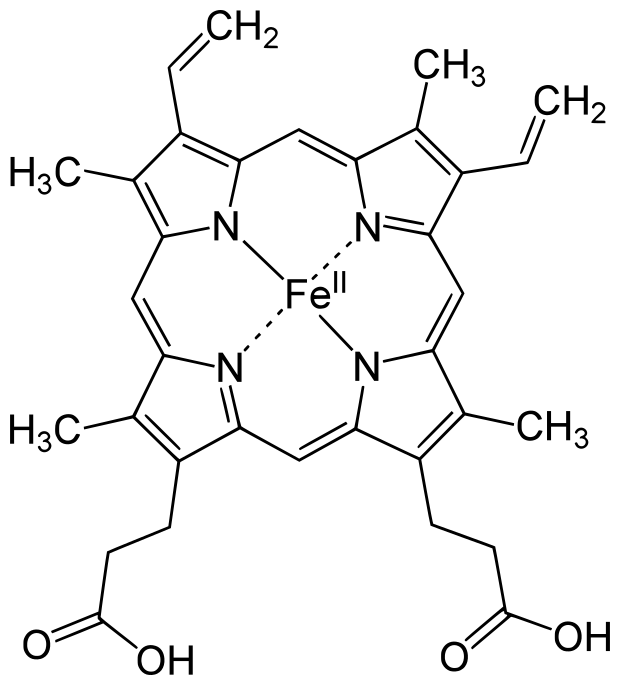
\includegraphics[width=0.5\linewidth]{figures/HEM} 

}

\caption{Heme-b (HEM)}\label{fig:structHEM}
\end{figure}
\begin{figure}

{\centering 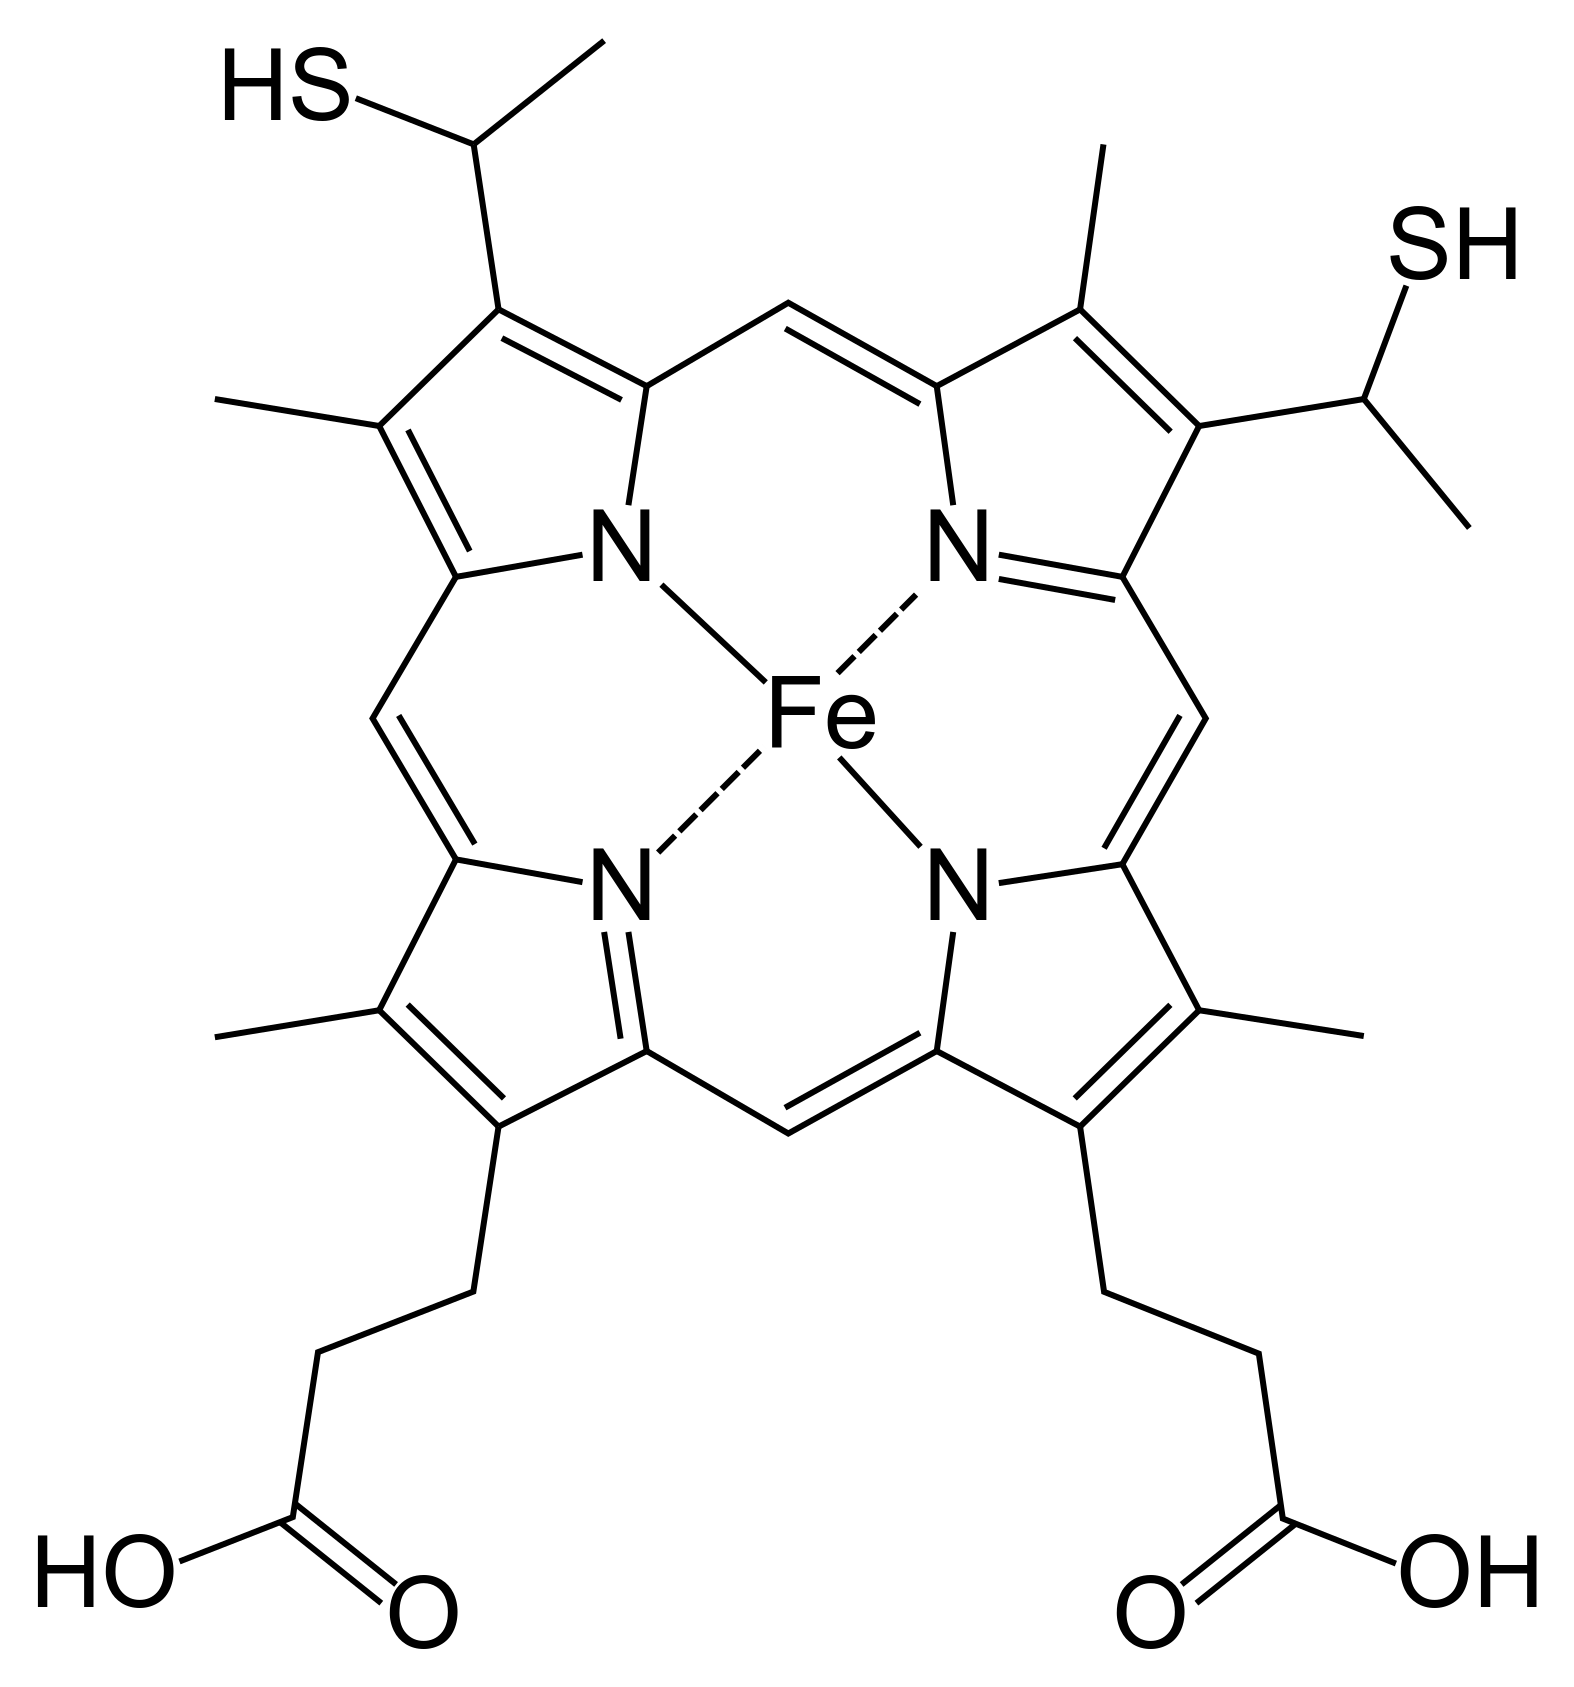
\includegraphics[width=0.5\linewidth]{figures/HEC} 

}

\caption{Heme-c (HEC)}\label{fig:structHEC}
\end{figure}

\begin{figure}

{\centering 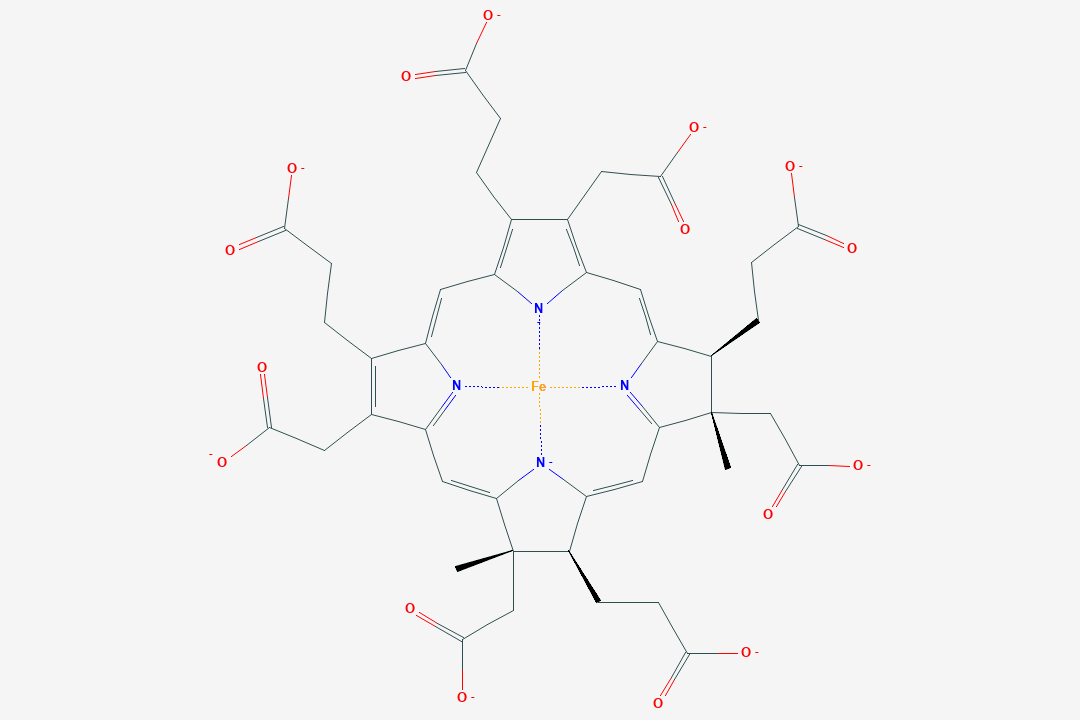
\includegraphics[width=0.5\linewidth]{figures/SRM} 

}

\caption{Siroheme (SRM)}\label{fig:structSRM}
\end{figure}

\begin{figure}

{\centering 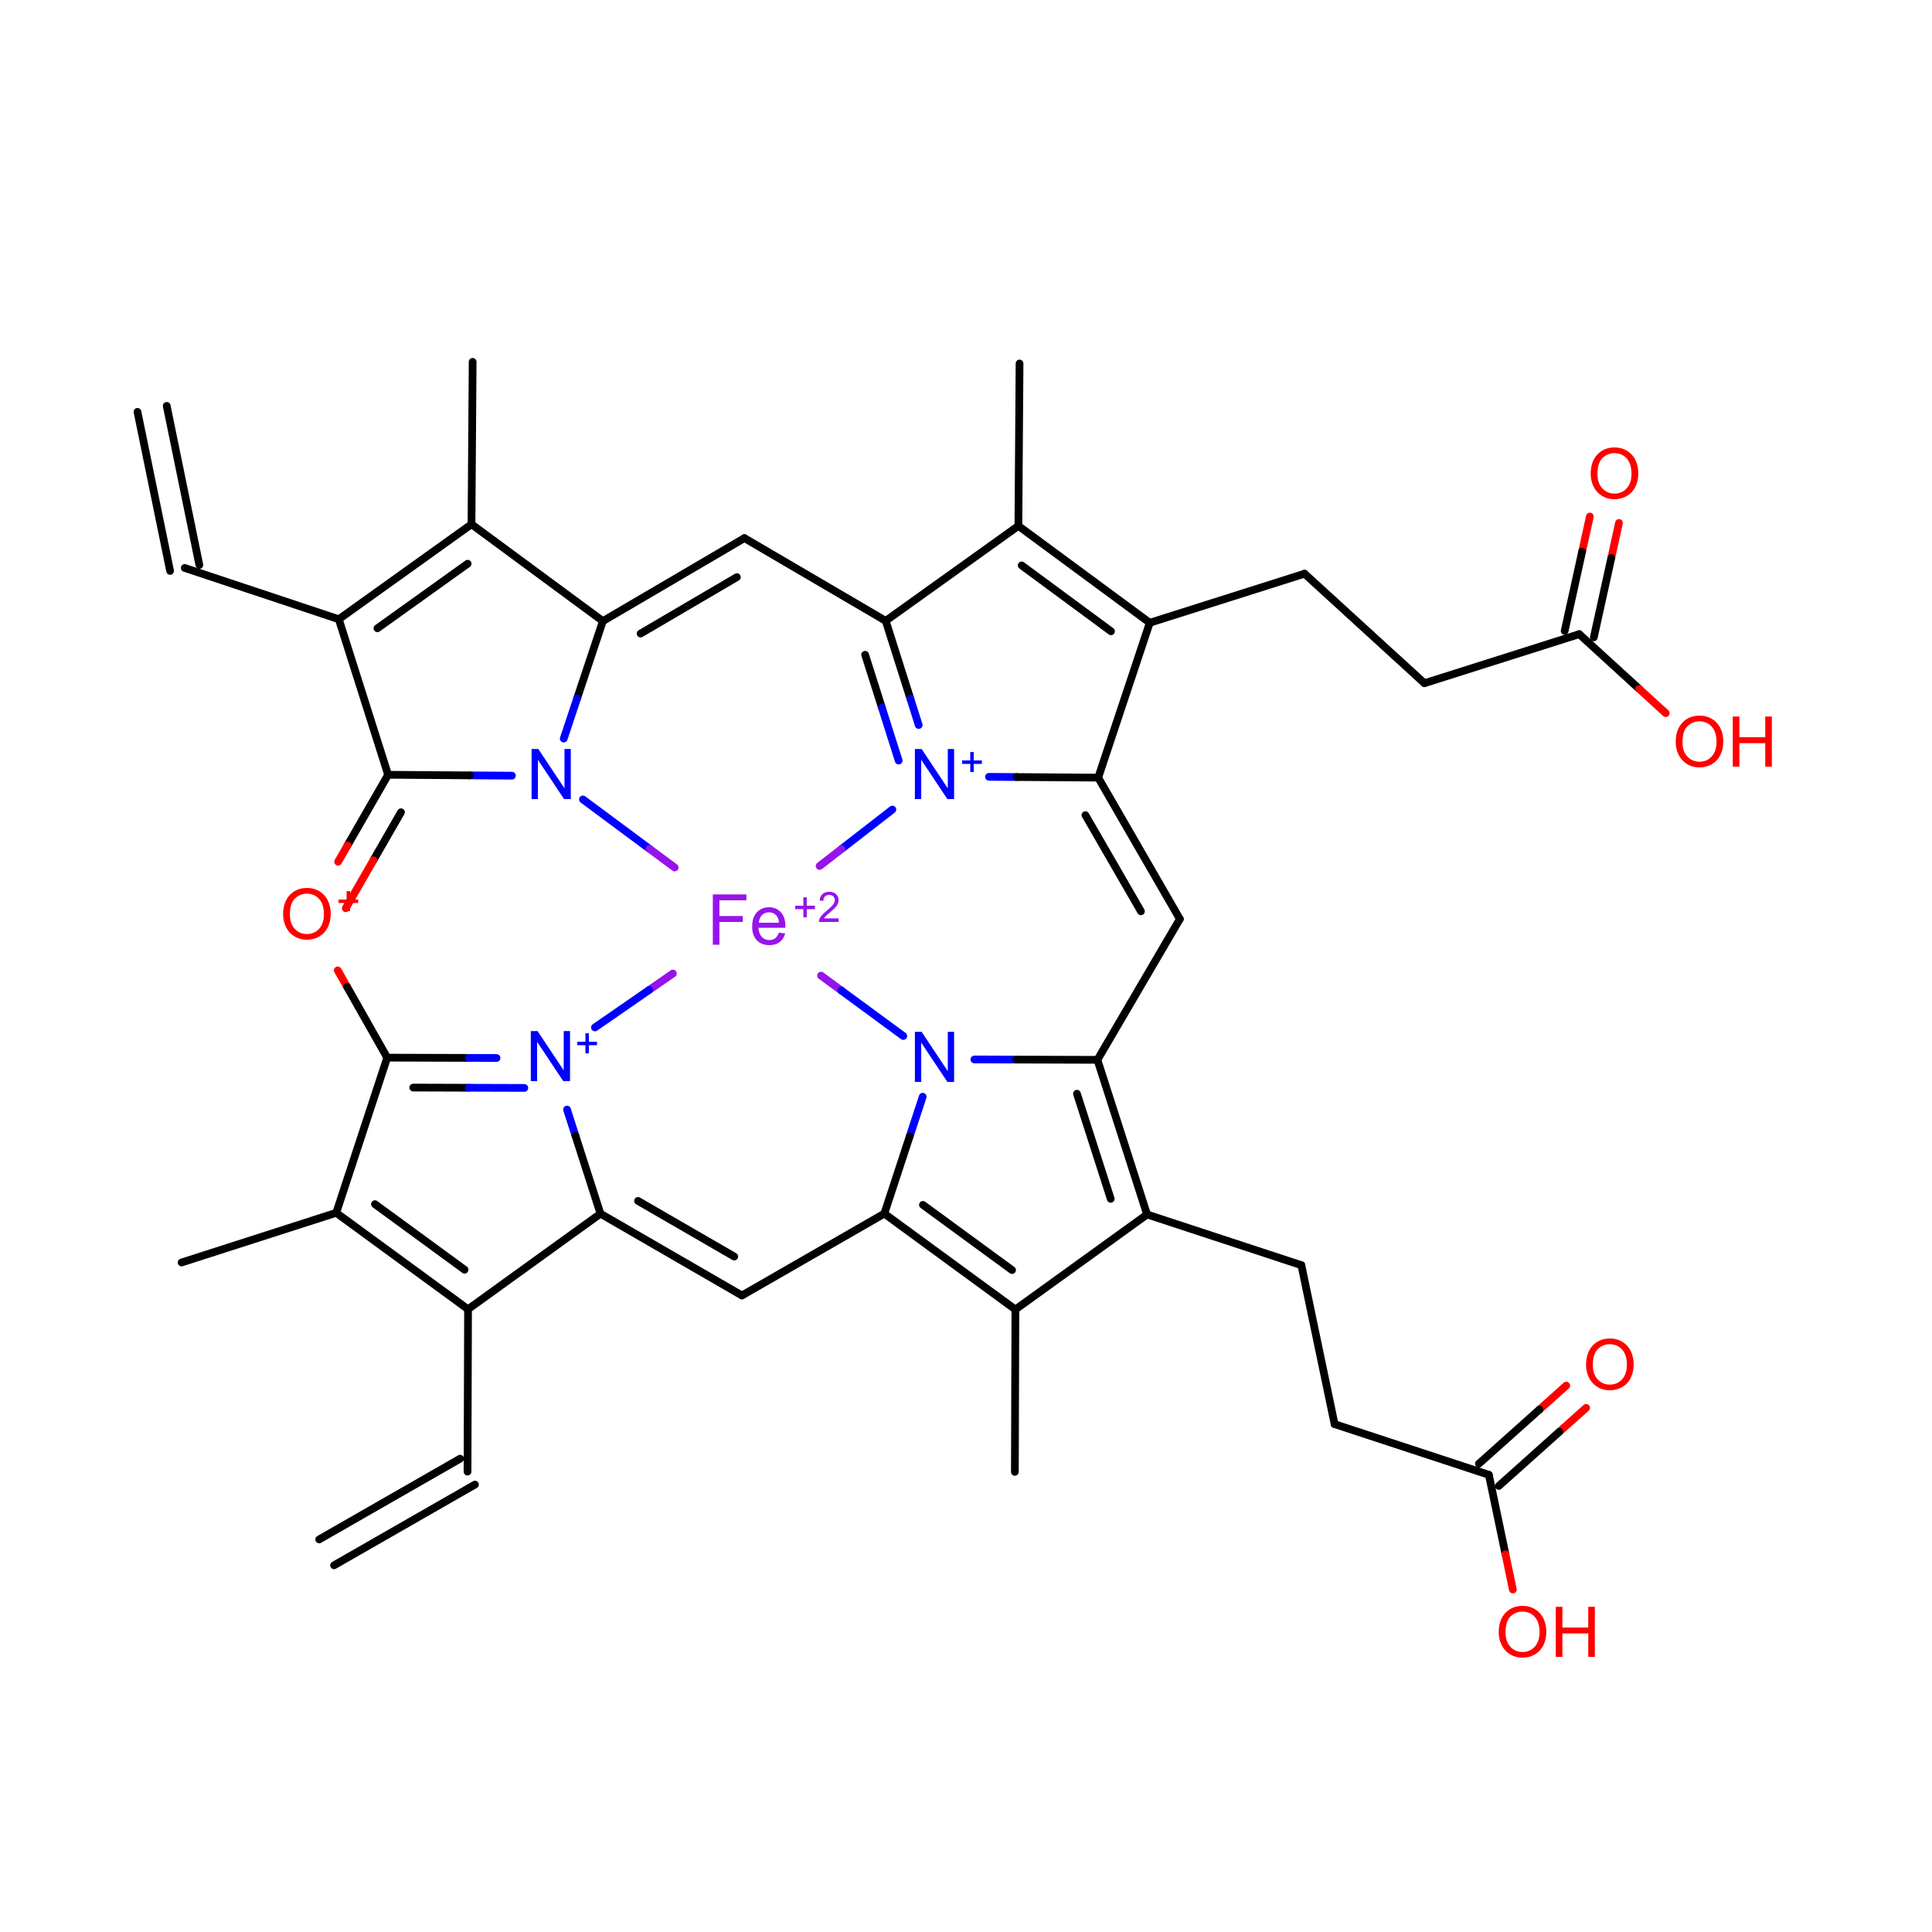
\includegraphics[width=0.5\linewidth]{figures/VEA} 

}

\caption{Verdoheme, VEA}\label{fig:structVEA}
\end{figure}
\begin{figure}

{\centering 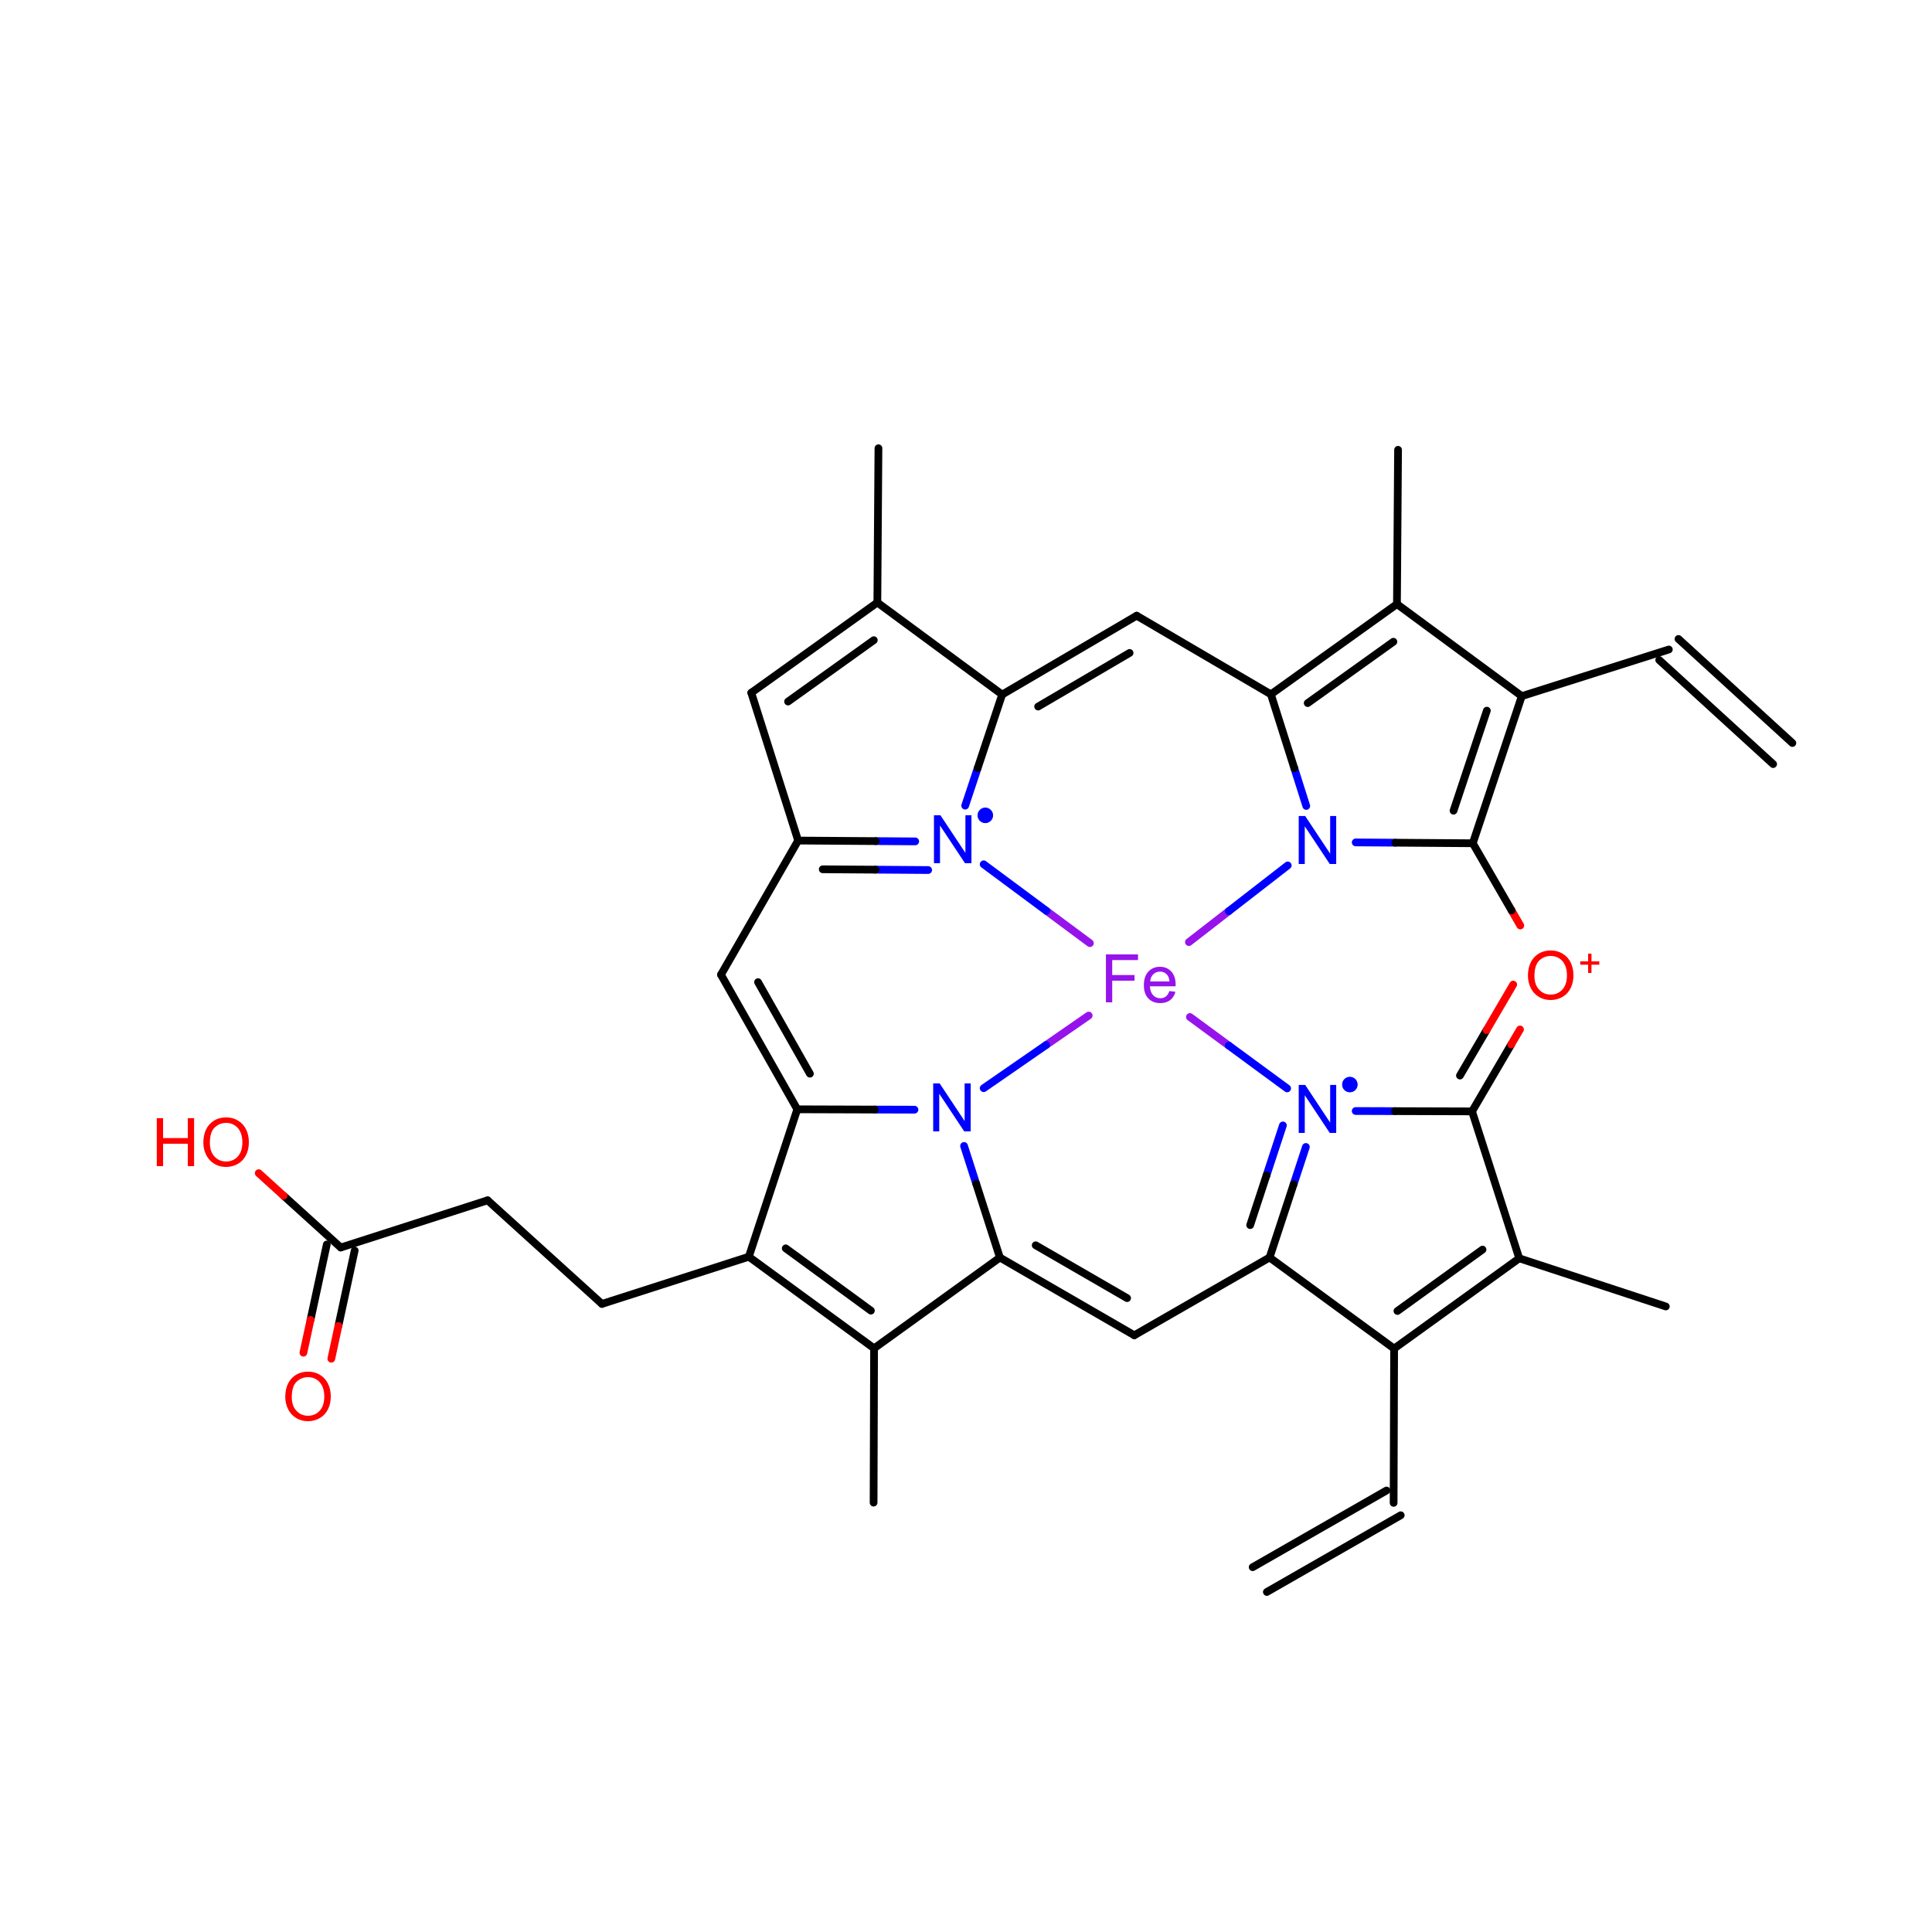
\includegraphics[width=0.5\linewidth]{figures/VER} 

}

\caption{Verdoheme, VER}\label{fig:structVER}
\end{figure}

\#\#Types of Heme

The most common heme is heme-b. It is employed by the vast majority of hemoproteins. It is composed of an iron and porphyrin ring complex, with the addition of two propionate groups. These two propionate groups interact with polar amino acids in the binding pocket. The iron atom is usually coordinated to a histidine or cysteine, depending on the enzyme.

Heme-c is derived from heme-b. It is fairly similar to heme, with two notable excetions: the iron atom binds, with few exceptions, covalently to cysteine residues in the binding pocket; and its two vinyl groups form thioester bonds with amino acids in the protein binding pocket. Its function is much more specific than heme-b, mostly serving as an electron carrier rather than catalyzing a plethora of reactions. The reason for this is not abundantly clear, but several studies suggest that because of its covalent bonding, heme-c has an electronic potential that is can be far lower and in general more broad, and more specifiable, than heme-b. \autocite{Bowman2008,Kleingardner2015}

Siroheme is even more limted in its applications, but highly specialized for its role. It is still an iron atom-porphyrin coordination complex, but it contains far more carboxyl and propionate groups than the other types of heme, making it highly polar. It is used exclusively in sulfite and nitrite reductases, which catalyze the reduction of the sulfates and nitrates plants uptake from the ground, providing the sources of nitrogen and sulfur used to produce nitrogen and sulfur-containing amino acids(\textcite{Tripathy2010}). The reason for the use of siroheme in this reaction rather than heme-b is not completely understood. But one study suggests that the bridge that siroheme forms between its catalyic iron atom, and the protein matrix envrionment (which also necessarily involves another cofactor, a cluster of cubane for electron transfer and provision) is more efficient at channeling electrons than the bridge that could be formed by heme.\autocite{Branzanic2019}

Lastly, verdoheme is an intermediate product in the degradation of heme-b by heme oxygenase. When heme oxygenase degrades heme-b, biliverdin, carbon monoxide, and iron are produced; verdoheme is the precusor to bilverdin\autocite{Lai2010,Sato2007}. While a product of prior reactions wthin heme oxygenase, verdoheme appears to be oriented and bound differently \autocite{Lad2004}. The two structures used in the study, VEA and VER, are either partially oxidized or partially oxidized and contain one less propionate group.

In summary, heme molecules are varied, and used in a diverse set of reactions. Several enzymes have the potential to be of great value either in biocatalysis or pharmaceutical applications. There are multiple methods employed to design molecules, but rational design in particular (basically, the mutation of certain residues based on an understanding of the structure-function relationships) is at least partially hampered by an incomplete understanding of the binding environment for heme. The importance of the binding environment was noted in a study seeking to design \emph{de novo} heme-c based enzymes, and found the binding environment likely to be of importance in modulating redox potential \autocite{Ishida2004}.

A fairly recent study conducted a structural analysis of 125 hemoprotein chains(\textcite{Li2011}). The study suggested hemoproteins undergo small conformational changes during binding; and that apo-form (ligand-containing) proteins may therefore be suitable for bioinformatics-based prediction and protein design. Additionally, the heme binding environment of the protein dataset used in the study was found to be rich in aromatic and nonpolar residues.

The aforementioned study was published in 2011 - since then the PDB has been populated with far more hemoproteins. The 125 protein chains used in the study were sourced from a small dataset of proteins (FIXME: Double check but their Table 2 is like 20 proteins), compared to the amount of hemoproteins now available in the PDB. The focus of the study was on conformational differences induced by heme-binding. And as for the binding environment, the focus was largely on interactions with the coordinating iron atom rather than interactions that occur with the porphyrin ring. \textbf{could add the distances arbitrary definition thing but I hesitate to write anything that could be construed as uh, negative}

The interactions heme forms with its binding environment have been well documented. And many studies have demonstrated the importance of these interactions and have either demonstrated or at least furnished theoretical mechanisms by which the heme molecule functions in reactions involving hemoproteins. However, there has not been significant work dedicated to examining the heme-binding environment itself.

In this study, we present research focused on elucidating the binding environment of multiple heme molecules: heme-b (HEM), heme-c (HEC), siroheme (SER), and verdoheme (VEA/VER). UCSF Chimera was used to both extract and predict properties of a diverse set of hemoproteins. R was used to analyze the results. A robust and high-throughput framework was constructed to process the datasets for each heme molecule, requiring only inputs of which ligand is to be examined per dataset.

The properties extracted and predicted of the heme molecules were (I need to figure out how to do a bullet list in this format):
+Amino acid frequencies within binding pockets
+Volumes
+Solvent accessible and excluded surface areas of heme and binding pockets
+Distances of amino acids from the Fe atom of heme
+Planar angles of amino acids in binding pocket v. heme
+CA-CB-Fe angles of amino acids in binding pocket v. heme

These results may be of use in rational design of hemoproteins in future studies, or at least improve the understanding of the heme binding environment.

\textbf{WILL INSERT PARAGRAPH ABOUT THE MEANING OF THESE RESULTS IN THE DESIGN ARTIFICAL METALLOPROTEINS, AND BRIEFLY INTRODUCE THEM EARLIER. `AS MENTIONED PREVIOUSLY, THERE ARE MANY OPPORTUNITIES TO EMPLOY IMPROVED HEMOPROTEINS, AND A MORE THOROUGH UNDERSTANDING OF THE HEME BINDING ENVIRONMENT WOULD AID IN THEIR DESIGN\ldots{}'}

\adjustmtc
\markboth{Methods}{}

\hypertarget{methods}{%
\chapter{Methods}\label{methods}}

\hypertarget{datasets}{%
\section{Datasets}\label{datasets}}

\noindent A list of PDBs was assembled that represented either a representative sample of a variety of proteins, with a resolution better than 3A, (HEM and HEC) or, all proteins containing these ligands were downloaded from the PDB (in the case of SRM, VER, VEA). Not all downloaded PDBs were appropriate for this study (e.g.~contained ``wobble'' structures) and therefore the amount of PDBs was culled. The datasets are current as of 16 August 2021.

The size of the datasets actually used in the study were as follows: HEM (n=58), HEC(n=14), SRM (n=9), VER (n=2) and VEA (n=2) for a combined n=4 for VERDOHEME.

The name of all proteins used in the study and their source organism are provided tables within Appendix \ref{molOrgSec}.

\hypertarget{preprocessing}{%
\section{Preprocessing}\label{preprocessing}}

Many of the PDBs downloaded were multimeric structures. While many of the scripts employed in the study may function with multimeric structures, the number of subunits per protein (FIXME! better way to say this?) would skew results in favor of multimeric proteins with more subunits. The information gleaned from similar subunits would also not be of utility in this study.

Therefore all downloaded PDBs were converted to monomeric structures. This was achieved by saving a single chain (chain A) of each PDB and eliminating all other chains. The single chain was then saved as a PDB and used in all subsequent scripts.

\hypertarget{processing-monomers}{%
\section{Processing Monomers}\label{processing-monomers}}

UCSF-Chimera was used to generate all data in this study. Multiple scripts were employed to achieve a high-throughput process where all monomeric PDBs could be processed in the same session.

Chimera was used to predict the following qualities: Volume of the ligand binding pocket, accessible and excluded surface area of the ligand, and accessible and excluded surface area of the binding pocket. These calculations require a population of atoms to be selected for the calculation.

Atoms were selected within a distance cutoff, to be considered as ``interacting'' with the ligand or forming the binding pocket. Distance cutoffs from the ligand of 5A and 7A were chosen; for the predicted qualities, the algorithms were run twice to get values at 5A and 7A. For the distance and angle calculations, only the 7A distance cutoff was used, as the cutoff does not factor into any calculations and may be set during analysis.

as these are selected arbitrarily, data from the 5A and 7A runs are overlaid in the figures reported in Appendix \ref{Figures}. Data tables are also provided in Appendix \ref{Tables}.

\hypertarget{amino-acid-frequency}{%
\subsection{Amino Acid Frequency}\label{amino-acid-frequency}}

Amino acids within the bounds of the lower and upper distance cutoff were selected and recorded. These were then counted for frequency per residue.

\hypertarget{volume-calculations}{%
\subsection{Volume Calculations}\label{volume-calculations}}

Volume of the binding pocket was predicted via Surfnet, run with default parameters of Grid Interval = 1.0 and Distance Cutoff = 10.0 (the latter option does not relate to the distance cutoff from the ligand(FIXME! find source for this, appears 100\% to be true?)).

\hypertarget{surface-area-calculations}{%
\subsection{Surface Area Calculations}\label{surface-area-calculations}}

Excluded and accessible surface areas of both the ligand and the binding pocket were calcualted using Chimera's ``surf'' algorithm, available as ``Measure Volume and Area'' via the GUI.

\hypertarget{distance-calculations}{%
\subsection{Distance Calculations}\label{distance-calculations}}

Distances of amino acids from the ligand could not be calculated accurately nor precisely in a direct way. Instead, distances for each atom composing a residue were calculated. The distances of all atoms within a residue were averaged, and this value was taken as the mean distance of the entire residue and used in subsequent steps.

The data produced in this step therefore include the mean distance of each amino acid. This is traceable, and the angular data below are cross-referenced with this list of distances. All data shown in figures (FIME! Also for tables?) are multidimensional and may be filtered for distance.

\hypertarget{planar-angle-calculations}{%
\subsection{Planar Angle Calculations}\label{planar-angle-calculations}}

Individual residues and the ligand were defined as axes The angle between each residue's axis and the axis of the ligand were calculated. Each axis functions essentially as a separate plane. (FIXME! Include a picture of what this looks like?) This employed the ``define axis'', and ``angle'' functions of Chimera; the Axes/Planes/Centroids Structural Analysis function of Chimera via GUI.

\hypertarget{ca-cb-fe-calculations}{%
\subsection{CA-CB-Fe Calculations}\label{ca-cb-fe-calculations}}

Residues within the distance cutoff were examined one by one. The angle of between each residue's carbon alpha (CA) and carbon beta (CB) and the Fe of the ligand was calculated, using the ``angle'' function of Chimera. The ligand nor the Fe atom were compared with themselves.

\hypertarget{import-to-r}{%
\section{Import to R}\label{import-to-r}}

All data were imported to R and processed from text files into organized data formats. R was used to cross-reference angle and distance data. All plots and tables were constructed using R and imported directly to this document using Rmarkdown.

\adjustmtc
\markboth{Introduction}{}

\adjustmtc
\markboth{Methods}{}

\hypertarget{discussion}{%
\chapter{Results and Discussion}\label{discussion}}

\minitoc

--\textgreater{}

\hypertarget{analysis-of-nearby-residues-of-natural-porphyrins}{%
\section{Analysis of Nearby Residues of Natural Porphyrins}\label{analysis-of-nearby-residues-of-natural-porphyrins}}

The first part of the study aimed at providing statistics on the amino acid propensity to interact with hemes in natural proteins. We studied heme-b, heme-c, siroheme and verdoheme. Because we are not looking only at the iron environment, but instead at the environment of the entire microcycle, we did the analysis for any amino acid with potential contact with the heme. This was defined as any AA having at least one atom within the cutoff distances of 5 and 7 Angtroms (A).

Amino acid frequencies were obtained for distance cutoffs of 5A and 7A - these figures and data are shown in \textbf{FIXME ADD APPENDICES LATER} The trends in these data are very similar and therefore only the data pertaining to the 7A distance cutoff are discussed below.

\hypertarget{disc-aaFreq}{%
\section{AA Frequency}\label{disc-aaFreq}}

\hypertarget{heme-b}{%
\subsection{Heme-b}\label{heme-b}}

\hypertarget{amino-acid-frequencies-in-binding-pocket}{%
\subsubsection{Amino Acid Frequencies in Binding Pocket}\label{amino-acid-frequencies-in-binding-pocket}}

Figure \ref{fig:HEM-AAfreq} plots the frequency of each residue within 7A of heme-b. Immediately below is Figure \ref{fig:HEM-AAfreqAll}, which plots the frequency of each residue within the entire monomer. \textbf{I'm thinking put tables in back they dont add much value here} Data tables are available in Appendix\ldots{}

\begin{figure}
\centering
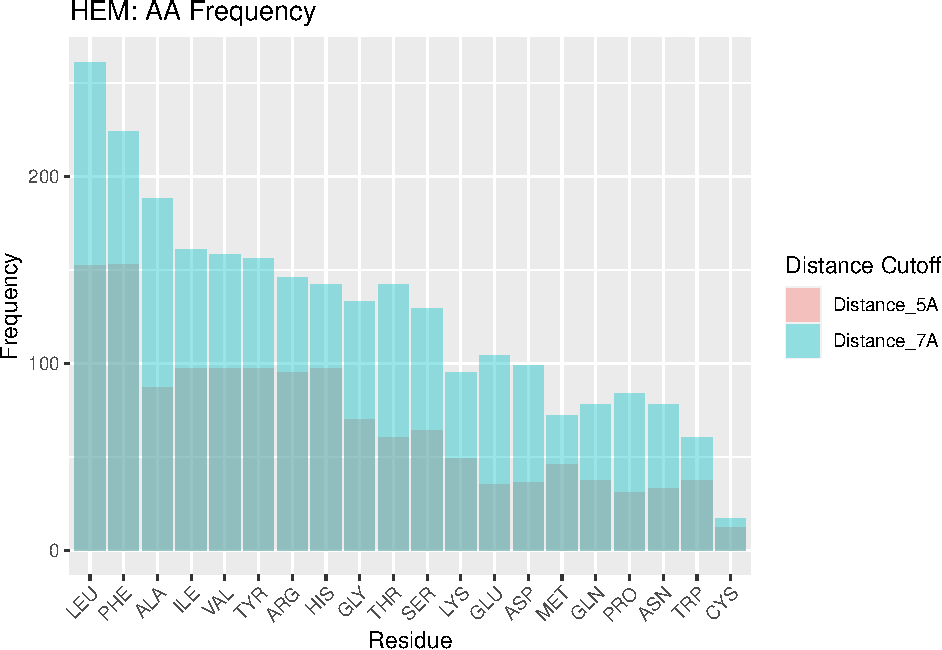
\includegraphics{_main_files/figure-latex/HEM-AAfreq-1.pdf}
\caption{\label{fig:HEM-AAfreq}HEM: AA Frequency within 7A}
\end{figure}

\begin{longtable}[t]{lr}
\caption{\label{tab:HEM-t-AAfreq}HEM AA Freq}\\
\toprule
Residue & Freq\\
\midrule
\endfirsthead
\caption[]{\label{tab:HEM-t-AAfreq}HEM AA Freq \textit{(continued)}}\\
\toprule
Residue & Freq\\
\midrule
\endhead

\endfoot
\bottomrule
\endlastfoot
\cellcolor{gray!6}{LEU} & \cellcolor{gray!6}{261}\\
PHE & 224\\
\cellcolor{gray!6}{ALA} & \cellcolor{gray!6}{188}\\
ILE & 161\\
\cellcolor{gray!6}{VAL} & \cellcolor{gray!6}{158}\\
\addlinespace
TYR & 156\\
\cellcolor{gray!6}{ARG} & \cellcolor{gray!6}{146}\\
HIS & 142\\
\cellcolor{gray!6}{THR} & \cellcolor{gray!6}{142}\\
GLY & 133\\
\addlinespace
\cellcolor{gray!6}{SER} & \cellcolor{gray!6}{129}\\
GLU & 104\\
\cellcolor{gray!6}{ASP} & \cellcolor{gray!6}{99}\\
LYS & 95\\
\cellcolor{gray!6}{PRO} & \cellcolor{gray!6}{84}\\
\addlinespace
ASN & 78\\
\cellcolor{gray!6}{GLN} & \cellcolor{gray!6}{78}\\
MET & 72\\
\cellcolor{gray!6}{TRP} & \cellcolor{gray!6}{60}\\
CYS & 17\\*
\end{longtable}

\textbf{I use `surprising, striking' a lot in this discussion. I'll reword this to have some variety later. The results are at least interesting!}

Beginning at the left of the figure and moving right, large, nonpolar amino acids appear most frequently within 7A: LEU and PHE; ILE appears less frequently than these two amino acids but nonetheless is in high frequency. Small, nonpolar amino acids ALA and VAL also appear very frequently. As the majority of the heme-b molecule is made up of the nonpolar porphyrin ring, these amino acids are therefore likely in such high frequency to provide the nonpolar interactions/environment with the pyrole groups and methyl and vinyl groups.

Tyrosine, arginine, histidine appear next most frequently. The two propionate groups on heme are used to coordinate the heme in the binding pocket. These polar residues are therefore likely interact with the propionate groups, providing the polar interactions necessary, in addition to the nonpolar interactions above, to provide as hospitable of a binding environment as possible to coordinate the heme. In additon, the arginine and histidine groups are positively charged (at pH 7),further facilitating interaction with the electronegative proprionate groups of heme-b. It should be noted histidine is one of the residues that coordinates the iron atom, and this may therefore inflate its frequency in the binding pocket.

Glycine is a small residue and cannot form significant interactions within its environment; however, its frequency, or lack thereof (compared to background frequency, discused later), suggests the binding pocket may not require as much flexibility or\ldots{} spatial considerations as in the rest of the protein. This would logically follow from the need for conserved binding sites.

Next appear serine, glutamate (glutamic acid) and aspartate (aspartic acid) and lysine. These are polar residues, and glutamate and aspartate are negatively charged; lysine is polarpositively charged. The negative charge is unlikely of importance in interaction with heme-b, however these polar amino acids likely again interact with the propionate groups on heme; only, infrequently. What is most interesting is why lysine is in such low abundance relative to the other polar, positively charged residues, arginine and histidine. Perhaps lysine's fairly linear structure prevents it from fitting into the binding pocket; however, arginine is also somewhat linear and features prominently. The exact reason for why this could be is beyond the scope of this study.

Proline is a small nonpolar amino acid in low frequency; the trend for heme-b, at least, appears to be to favor large nonpolar amino acids in the binding pocket. This may suggest that a large amount of nonpolar interactions, per residue, is favored in the binding pocket, perhaps because of the limited space available to position residues to interact with heme.

Asparagine and glutamine are both medium-sized polar amino acids; given the trends already discussed it is surprising these are not in greater abundance. But as with proline, it may simply be a matter of maximizing the benefit of the interactions that may be formed with the heme; while asparagine and glutamine are polar, amino acids like arginine and histidine are both polar and positively charged, capable of stronger interactions with the electronegative propionate groups.

Methionine and tryptophan appear very infrequently in the binding pocket. All nonpolar amino acids already mentioned do not possess a sulfur (thio something?) bond in their structure; perhaps it is less favorable for the sulfur atom to interact with the porphyrin ring than another carbon \textbf{HELP I'M AT A LOSS ON EXPLAINING THIS ONE}. Tryptophan is very surprising to find as second-to-least frequent. It is a large nonpolar amino acid - but perhaps its single, potential hydrogen bond, although weak, is enough to prefer completely nonpolar residues. Or, with its size, it is preferable to have more numerous, smaller nonpolar residues that can favorably interact with the porphyrin while reducing steric hindrance of other residues in the environment (taking up less space).

Cystine appears most infrequently of all the amino acids in the binding pocket. This is quite surprising - cystine is highly evolutionarily conserved to coordinate the iron in the binding pocket. Perhaps the sample of PDBs used in this study mostly use histidine to coordinate the iron - but this would only account for one residue in the binding pocket per pdb. Therefore these results suggest that while cystidine may be well suited to coordinate the iron in heme, it is poorly suited to form any nonpolar interactions with the porphyrin ring, leaving the task up to other, more suitably/intensely nonpolar amino acids.

Moving away from discussing individual amino acid populations, what is especially notable of the data for heme-b is that nonpolar residues appear in much greater frequency than polar residues. Nonpolar interactions with heme are therefore more numerous than polar interactions; quite logical, given there are only two polar propionate groups on a large porphyrin ring that is otherwise nonpolar. Their multiplicity may also suggest that they are potentially of greater importance than previously thought. At the very least, these results suggest that polar interactions and coordination of the iron atom, while necessary for heme binding, are insufficient, and that nonpolar intercations and the population of nopolar residues in the binding pocket should be considered when examining the binding environment of heme.

\hypertarget{comparison-with-background-amino-acid-frequencies}{%
\subsubsection{Comparison with Background Amino Acid Frequencies}\label{comparison-with-background-amino-acid-frequencies}}

While the frequencies of amino acids in the binding pocket have been discussed, it may also be of interest to compare against the background amino acid frequency, the general frequency of amino acids within the entire monomer. The degree to which this may affect the significance of the frequencies of the amino acids in the binding pocket is unclear - those amino acids are still employed and placed such as to bind the heme, rather than being a random assortment of residues. However, a in depth examination of simlarities and differences may reveal that some amino acids may simply be extremely highly conserved by chance and by virtue of their numerous population, rather than some chemical benefit.

Figure \ref{HEM-AAfreqAll} documents the frequencies of amino acids overall within the monomer.

Leucine and alanine as in the binding pocket frequencies are highly frequent in the overall monomer. This may suggest their prevalence in the binding pocket may simply be due to a high pulation of leucine and alanine in hemoproteins.

However, after these two amino acids the tendencies in frequency for the binding pocket and the monomer at large diverge.

Glycine is in high frequency - likely due to more complex geometry e.g.~helices outside the binding pocket. In interest of brevity, the remaining frequencies are summed up thus: the same trends that appear to exist in the binding pocket do not appear to exist in the monomer at large. While the order of frequencies in conserved binding pockets can be rationalized, justifying the overall frequencies in monomers invites significant speculation.

\begin{figure}
\centering
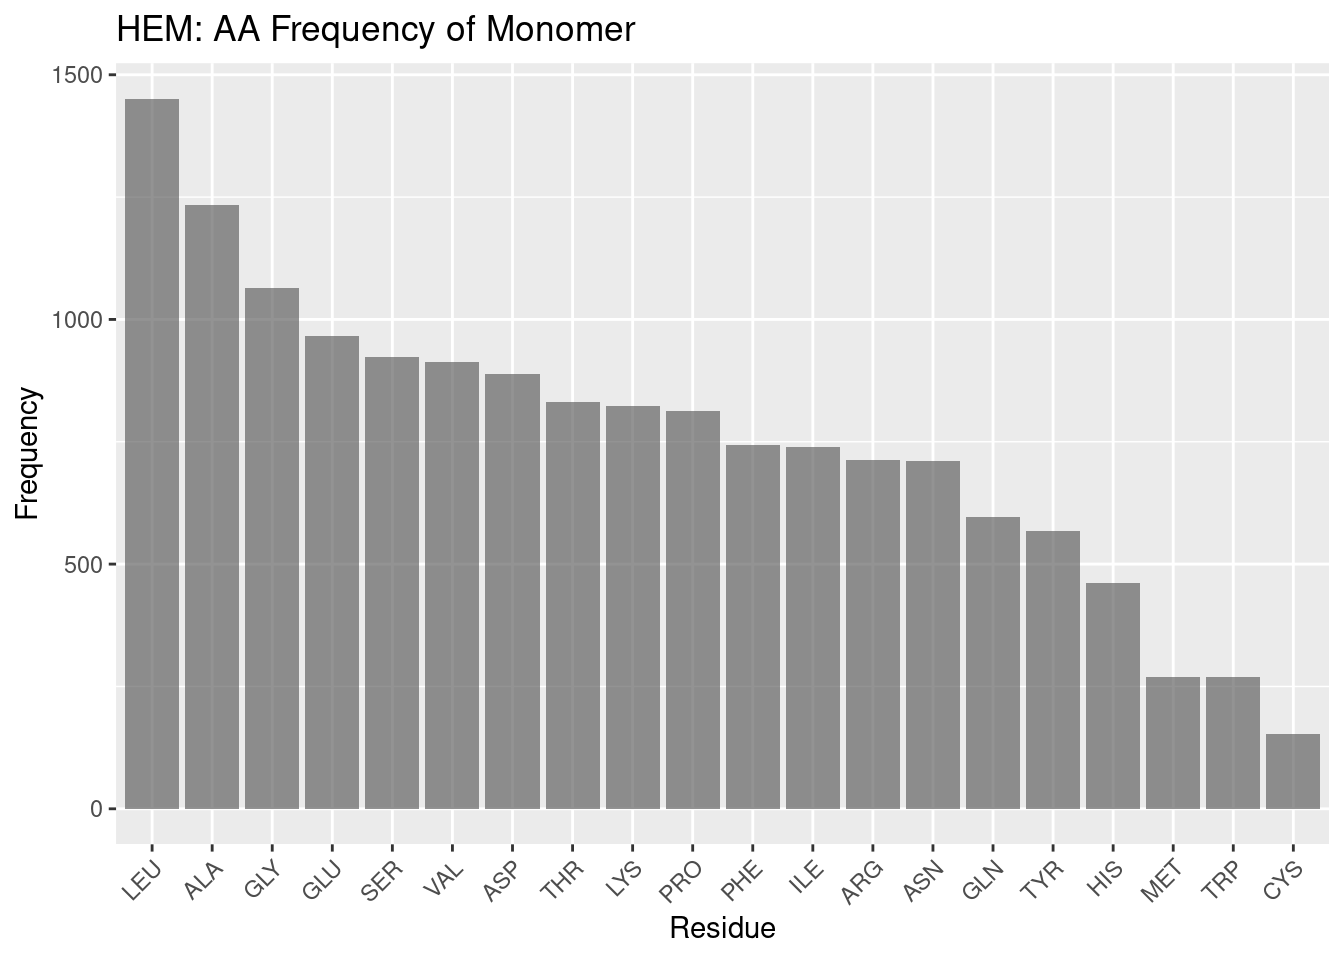
\includegraphics{_main_files/figure-latex/HEM-AAfreqAll-1.pdf}
\caption{\label{fig:HEM-AAfreqAll}HEM: AA Frequency of Monomer}
\end{figure}

\hypertarget{distributon-of-amino-acids-over-distance}{%
\subsubsection{Distributon of Amino Acids over Distance}\label{distributon-of-amino-acids-over-distance}}

After an exhaustive exploration of the relative frequencies of amino acids in the binding pocket, the figure below is fairly straightfoward. Figure \ref{fig:HEM-AAdist} plots the distribution of amino acids in the binding pocket against their distance from the iron of the heme.

We find that only a few residues come in close contact (\textless4A) of the heme: Cys, His, Tyr. Most residues center their distribution at around 6A, although Lys seems more biased than the remaining residues to be a bit closer. Cystidine and histidine may be at least in part explained to be close due to their use as coordnating residues; histidine, being in greater frequency, may also be this close due to favorable interactions with the porphyrin ring.

The proximity of tyrosine however, is lkely more notable. It cannot form coordination bonds with the heme iron, but tyrosine residues do interact with the propionate groups; and these results suggest that of all potentially interacting polar/positively charged residues, tyrosine is the most likely at least to be in close proximity to the heme molecule. Whether this illustrates an extreme imortance of tyrosine to interact with propionate groups, or instead the need for tyrosine to be in close proximity in order to form such interactions, is beyond the scope of this study.

\begin{figure}
\centering
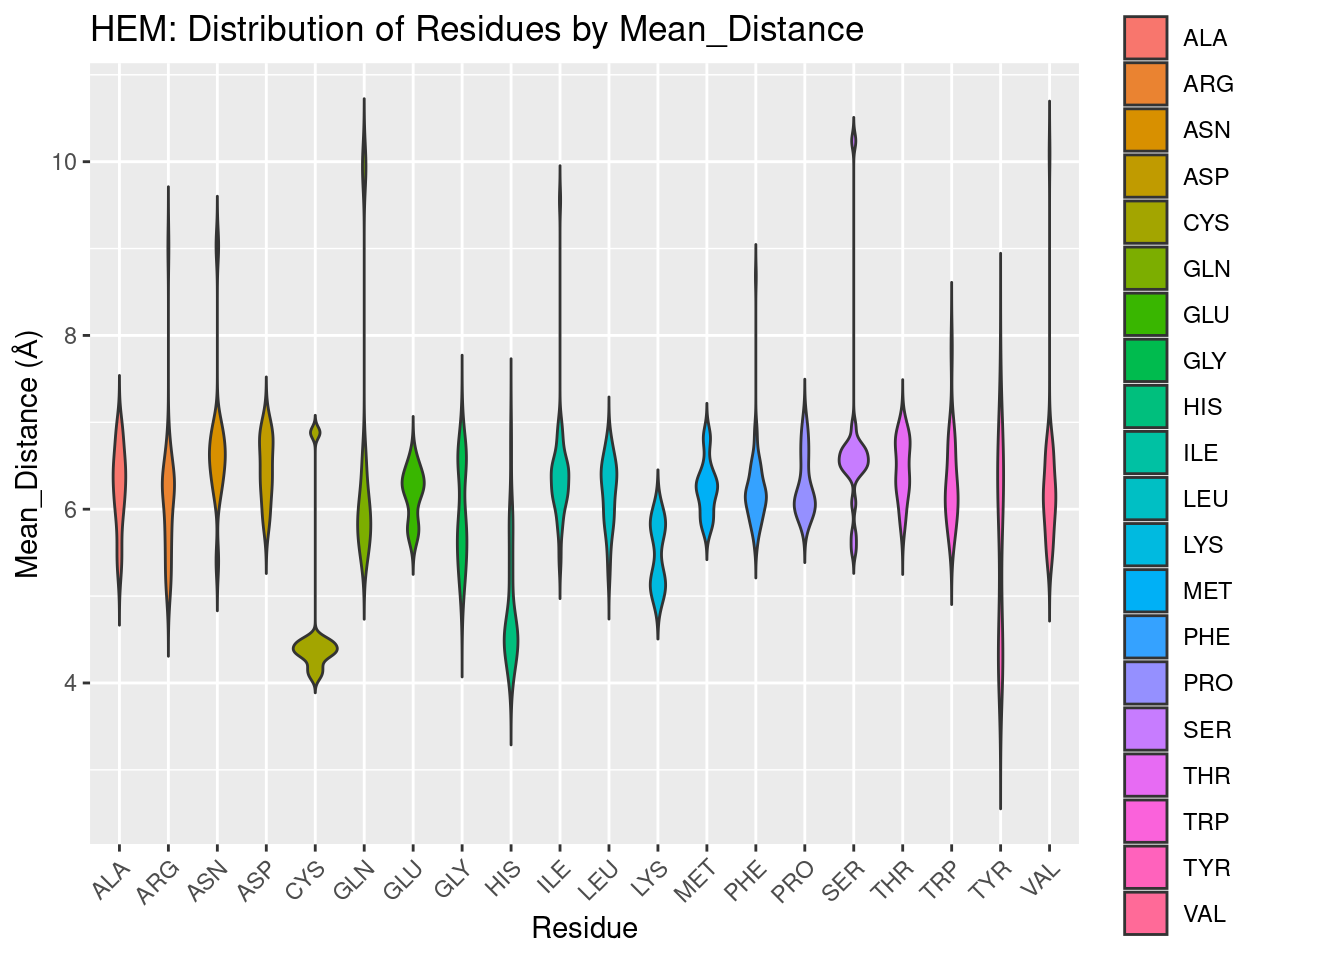
\includegraphics{_main_files/figure-latex/HEM-AAdist-1.pdf}
\caption{\label{fig:HEM-AAdist}HEM: AA Distances}
\end{figure}

\hypertarget{heme-c}{%
\subsection{Heme-c}\label{heme-c}}

\begin{figure}
\centering
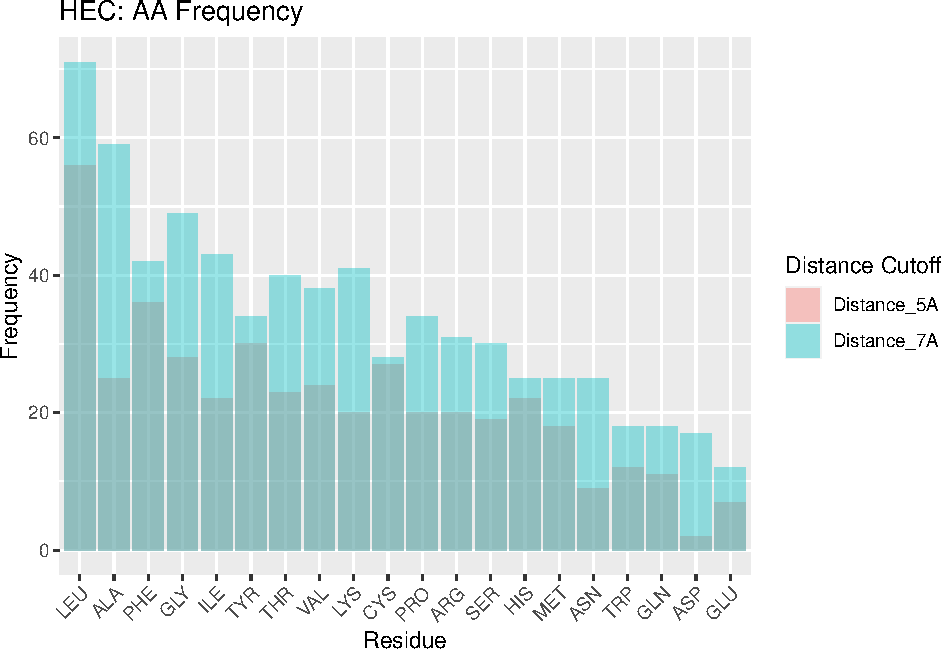
\includegraphics{_main_files/figure-latex/HEC-AAfreq-1.pdf}
\caption{\label{fig:HEC-AAfreq}HEC: AA Frequency}
\end{figure}

\begin{longtable}[t]{lr}
\caption{\label{tab:HEC-t-AAfreq}HEC AA Freq}\\
\toprule
Residue & Freq\\
\midrule
\endfirsthead
\caption[]{\label{tab:HEC-t-AAfreq}HEC AA Freq \textit{(continued)}}\\
\toprule
Residue & Freq\\
\midrule
\endhead

\endfoot
\bottomrule
\endlastfoot
\cellcolor{gray!6}{LEU} & \cellcolor{gray!6}{62}\\
ALA & 47\\
\cellcolor{gray!6}{GLY} & \cellcolor{gray!6}{39}\\
LYS & 38\\
\cellcolor{gray!6}{PHE} & \cellcolor{gray!6}{35}\\
\addlinespace
VAL & 35\\
\cellcolor{gray!6}{ILE} & \cellcolor{gray!6}{34}\\
THR & 34\\
\cellcolor{gray!6}{TYR} & \cellcolor{gray!6}{30}\\
ARG & 26\\
\addlinespace
\cellcolor{gray!6}{PRO} & \cellcolor{gray!6}{26}\\
CYS & 24\\
\cellcolor{gray!6}{MET} & \cellcolor{gray!6}{23}\\
HIS & 21\\
\cellcolor{gray!6}{SER} & \cellcolor{gray!6}{21}\\
\addlinespace
ASN & 20\\
\cellcolor{gray!6}{GLN} & \cellcolor{gray!6}{17}\\
ASP & 14\\
\cellcolor{gray!6}{TRP} & \cellcolor{gray!6}{12}\\
GLU & 11\\*
\end{longtable}

Leucine and alanine again are highly frequent for HEC, followed by quite similar trends and therfore HEC will not be as thoroughly discussed as HEM. The most notable differences may be that GLY and CYS are in far higher frequency than in heme. Heme-c almost always covalently binds to CYS, and this may explain that frequency: but as for the high frequency of glycine, perhaps the covalent binding of CYS is sufficient for other interactions to be of `lower priority', and the flexibility and shape of the binding pocket to be prioritized, therefore leading to more glycines being included in order to shape the pocket favorably. A note on this last part: \textbf{I feel like this is grasping at straws without much support, add more qualifiers or remove}

\hypertarget{comparison-to-background-frequency}{%
\subsubsection{Comparison to background frequency}\label{comparison-to-background-frequency}}

\begin{figure}
\centering
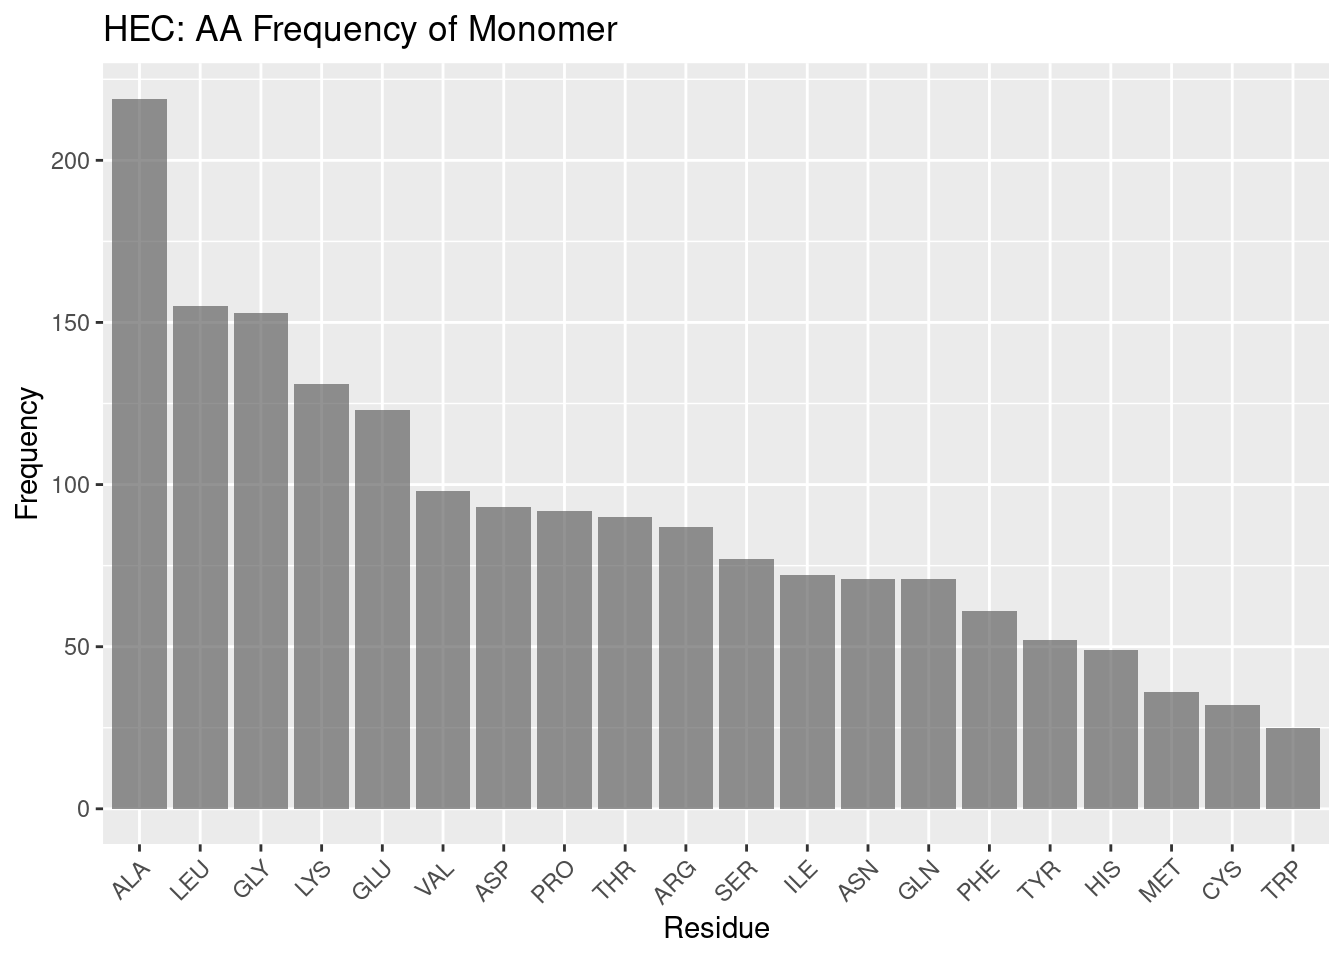
\includegraphics{_main_files/figure-latex/HEC-AAfreqAll-1.pdf}
\caption{\label{fig:HEC-AAfreqAll}HEC: AA Frequency of Monomer}
\end{figure}

Generally, the heme-c monomer is similar to the heme-b monomer, with a high frequency of alanine and leucine, followed by a divergence in the frequency of amino acids and therefore a struggle to form any meaningful discussion when it comes to comparing the binding pocket frequencies against background frequencies.

\hypertarget{aa-distribution-v.-distance}{%
\subsubsection{AA Distribution v. Distance}\label{aa-distribution-v.-distance}}

\begin{figure}
\centering
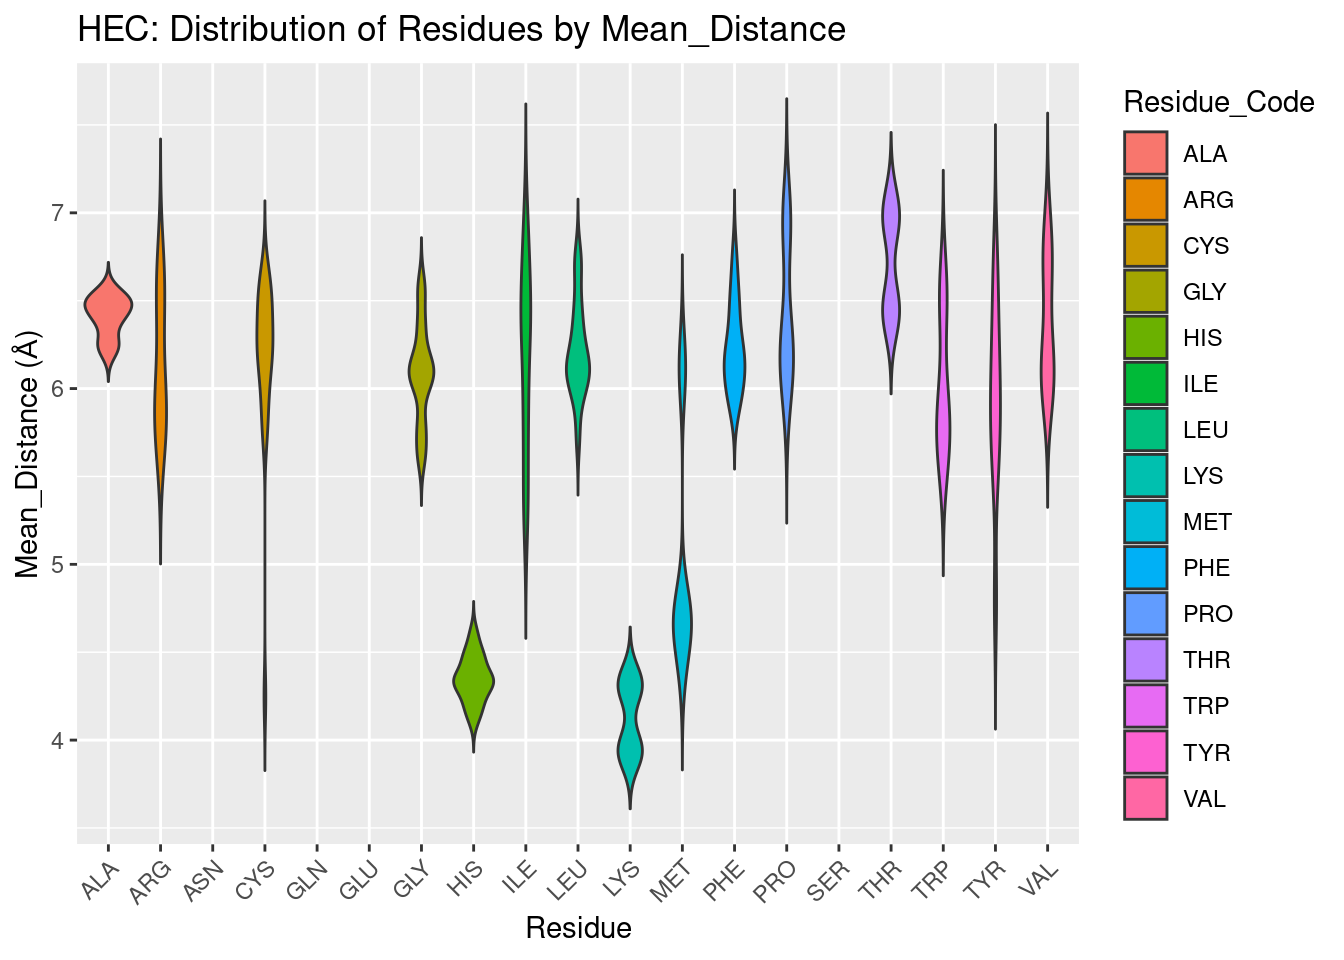
\includegraphics{_main_files/figure-latex/HEC-AAdist-1.pdf}
\caption{\label{fig:HEC-AAdist}HEC: AA Distances}
\end{figure}

The distribution of amino acids over distance from the heme iron for HEC is similar to HEM, with some exceptions. Cys, His, Tyr again are amongst the closest residues to HEC, likely for the same reasons of very strong polar interactions or coordination. Additionally, cysteine forms covalent, thioester bonds with heme-c, providing further justification for its proximity. However, for heme-c, lysine and methionine also are very proximal. The methionine residues are nonpolar and \textbf{HELP, NOT SO SURE WHY THEY'D BE SO CLOSE} Lysine is polar and positively charged, and therefore in the case of HEC being covalently bonded, and therefore reliably, specifically, positioned, the environment may be such that a lengthy, polar, charged residue may also be positioned well enough to be consistently nearby and forming interactions with the propionate groups.
\textbf{GRASPING AT STRAWS AGAIN}
\ldots. Maybe just leave it that for heme-c in particular, lysine and methionine appear favored. For good reason, they're nonpolar. But it's unclear why for heme-c these residues are employed but others aren't. I've left other sections like that.

\hypertarget{verdoheme}{%
\subsection{Verdoheme}\label{verdoheme}}

\textbf{Got some conflicting stuff here}

\begin{figure}
\centering
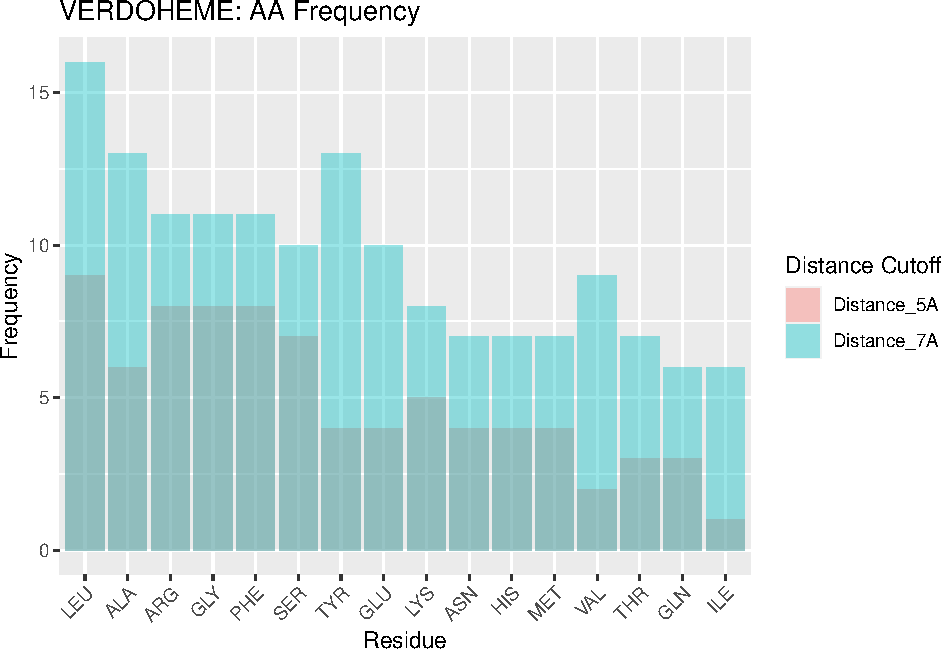
\includegraphics{_main_files/figure-latex/VERDOHEME-AAfreq-1.pdf}
\caption{\label{fig:VERDOHEME-AAfreq}VERDOHEME: AA Frequency}
\end{figure}

\begin{longtable}[t]{lr}
\caption{\label{tab:VERDOHEME-t-AAfreq}VERDOHEME AA Freq}\\
\toprule
Residue & Freq\\
\midrule
\endfirsthead
\caption[]{\label{tab:VERDOHEME-t-AAfreq}VERDOHEME AA Freq \textit{(continued)}}\\
\toprule
Residue & Freq\\
\midrule
\endhead

\endfoot
\bottomrule
\endlastfoot
\cellcolor{gray!6}{LEU} & \cellcolor{gray!6}{16}\\
ALA & 13\\
\cellcolor{gray!6}{TYR} & \cellcolor{gray!6}{13}\\
ARG & 11\\
\cellcolor{gray!6}{GLY} & \cellcolor{gray!6}{11}\\
\addlinespace
PHE & 11\\
\cellcolor{gray!6}{GLU} & \cellcolor{gray!6}{10}\\
SER & 10\\
\cellcolor{gray!6}{VAL} & \cellcolor{gray!6}{9}\\
LYS & 8\\
\addlinespace
\cellcolor{gray!6}{ASN} & \cellcolor{gray!6}{7}\\
HIS & 7\\
\cellcolor{gray!6}{MET} & \cellcolor{gray!6}{7}\\
THR & 7\\
\cellcolor{gray!6}{GLN} & \cellcolor{gray!6}{6}\\
\addlinespace
ILE & 6\\
\cellcolor{gray!6}{ASP} & \cellcolor{gray!6}{4}\\*
\end{longtable}

Verdoheme is dissimilar from HEM and HEC above. This is fairly surprising, given that verdoheme is an intermediate in the binding pocket for heme within heme oxygenases. The results discussed below may be attributable to the small sample size of verdoheme PDBs (n=4, combining VEA and VER), and should be appreciated with some skepticism. Nonetheless, the results will be discussed.

Leucine and alanine are again most frequent, but after this results diverge. Tyrosine and arginine are next most frequent - surprising, given that this is still the same pocket that bound heme. The data for heme-b indicate more frequent nonpolar residues before tyrosine. It is possible that heme's reorientation during its degradation moves it closer to another region of the binding pocket. Chemically, it may be that as heme is oxidized, there is greater need for polar interactions; this would help to explain the high frequency of polar residues.

Glycine is the next most frequent - it is in lower frequency, relatively, for heme-b\ldots. \textbf{I'm gonna hold off on discussing this further until I double check the paper that described heme's reorientation.}

\hypertarget{comparison-to-background-freq}{%
\subsubsection{Comparison to background freq}\label{comparison-to-background-freq}}

\begin{figure}
\centering
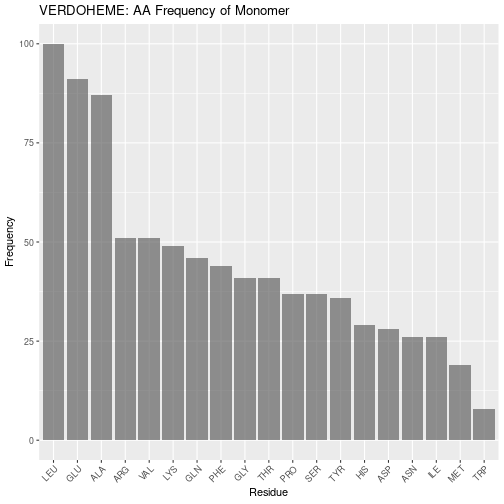
\includegraphics{_main_files/figure-latex/VERDOHEME-AAfreqAll-1.pdf}
\caption{\label{fig:VERDOHEME-AAfreqAll}VERDOHEME: AA Frequency of Monomer}
\end{figure}

\hypertarget{aa-distribution-over-distance}{%
\subsubsection{AA Distribution over distance}\label{aa-distribution-over-distance}}

\textbf{I'll double check why so few data appear here. I suspect it may be simply that there is not enough data/atoms to pull and form a decent enough graph.}
The highly conserved histidine for hemoproteins is exclusively within 5A for verdoheme. This result again suggests that at least some of the data for verdoheme may be highly biased because of the small sample size - heme-b data included a greater range for histidine. Nonetheless, this data suggests that verdoheme may be of different orientation during heme-b degradation, but is not spatially displaced far from the conserved binding site.

Glycine's proximity to verdoheme is just weird WTF.

\begin{figure}
\centering
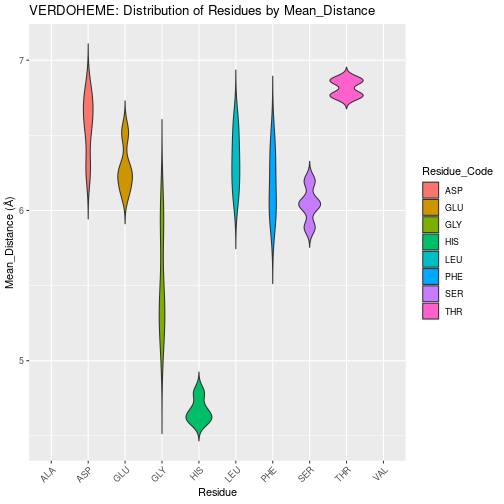
\includegraphics{_main_files/figure-latex/VERDOHEME-AAdist-1.pdf}
\caption{\label{fig:VERDOHEME-AAdist}VERDOHEME: AA Distances}
\end{figure}

\hypertarget{siroheme}{%
\subsection{Siroheme}\label{siroheme}}

\begin{figure}
\centering
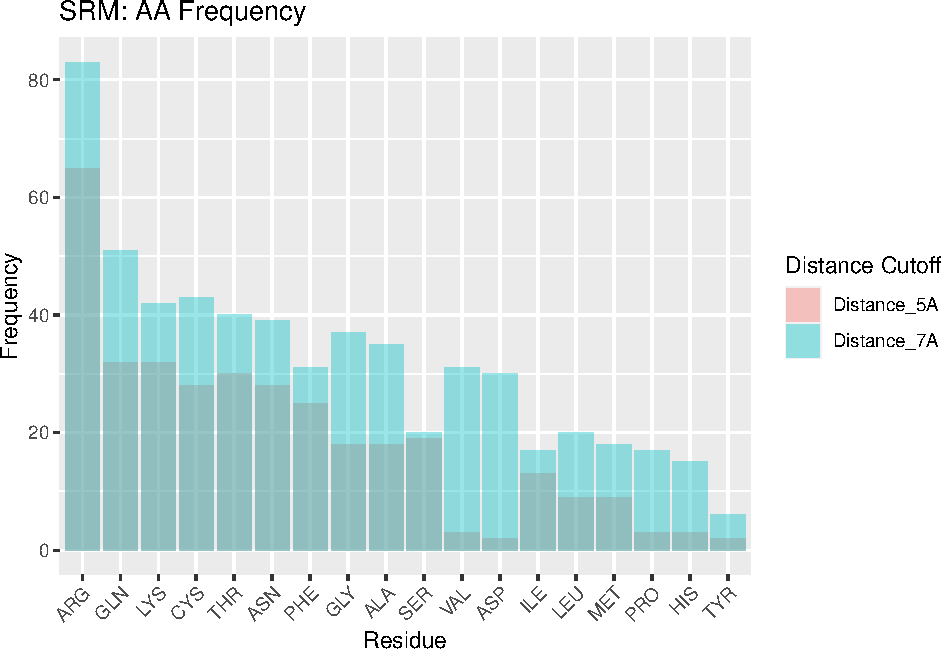
\includegraphics{_main_files/figure-latex/SRM-AAfreq-1.pdf}
\caption{\label{fig:SRM-AAfreq}SRM: AA Frequency}
\end{figure}

\begin{longtable}[t]{lr}
\caption{\label{tab:SRM-t-AAfreq}SRM AA Freq}\\
\toprule
Residue & Freq\\
\midrule
\endfirsthead
\caption[]{\label{tab:SRM-t-AAfreq}SRM AA Freq \textit{(continued)}}\\
\toprule
Residue & Freq\\
\midrule
\endhead

\endfoot
\bottomrule
\endlastfoot
\cellcolor{gray!6}{ARG} & \cellcolor{gray!6}{83}\\
GLN & 51\\
\cellcolor{gray!6}{CYS} & \cellcolor{gray!6}{43}\\
LYS & 42\\
\cellcolor{gray!6}{THR} & \cellcolor{gray!6}{40}\\
\addlinespace
ASN & 39\\
\cellcolor{gray!6}{GLY} & \cellcolor{gray!6}{37}\\
ALA & 35\\
\cellcolor{gray!6}{PHE} & \cellcolor{gray!6}{31}\\
VAL & 31\\
\addlinespace
\cellcolor{gray!6}{ASP} & \cellcolor{gray!6}{30}\\
LEU & 20\\
\cellcolor{gray!6}{SER} & \cellcolor{gray!6}{20}\\
MET & 18\\
\cellcolor{gray!6}{ILE} & \cellcolor{gray!6}{17}\\
\addlinespace
PRO & 17\\
\cellcolor{gray!6}{HIS} & \cellcolor{gray!6}{15}\\
TRP & 10\\
\cellcolor{gray!6}{TYR} & \cellcolor{gray!6}{6}\\
GLU & 2\\*
\end{longtable}

Siroheme, with a structure highly dissimilar to the other heme molecules examined, should be expected to have a different amino acid frequency profile - and indeed we confirm this in our results.

Nonpolar residues are not the most abundant in the siroheme binding pocket. In fact, disproportionately frequent to the rest of the residues in the binding pocket is arginine. Siroheme is saturated with carboxyl and propionate groups; the entire porphyrin ring surrounded by polar, electronegative groups. And therefore a polar, positively charged amino acid such as arginine is reasonable to expect in the binding pocket - what is striking, however is the extreme preference for arginine; such a profile does not exist for the other hemes.

Arginine is followed by other polar amino acids: glutamine, cystine, lysine (positively charged), threonine, and asparagine; a more homogenous trend than seen for the other heme molecules, in that there are no nonpolar residues at all in this first\ldots{} group of frequencies. \textbf{reword}. Though these results could be expected, they demonstrate the extent to which siroheme's binding pocket is dominated by polar residues. The preference for arginine out of all polar amino acids may be attributed to its positive charge, and very low pKa; lysine also has a positive charge and a low pKa (\textasciitilde10.5), but arginine's is much, much lower (\textasciitilde13.8) \textbf{fixme add citation} and it is able to form an additional hydrogen bond, and therefore reasonably dominates amongst the polar amino acids. Cysteine is used to coordinate the iron of siroheme, and while this did not significantly affect the frequency for other heme molecules, it is still possible this inflates the value for cysteine for siroheme.

After this group of polar amino acids, glycine is the next most frequent. Glycine has been situated at about a median frequency for other heme molecules, so perhaps its frequency here, slightly above the median, is of note. Only speculation is possible; perhaps ensuring the dominance of polar amino acids in the binding pocket requires extenive folding in the protein, therefore favoring glycine residues.

Finally we come to several nonpolar amino acids: alanine, phenylalanine, and valine. These amino acids define roughly the median of the frequency data. With all the polar groups on siroheme, it might be expected that only polar interactions would be desirable. However, the not miniscule frequency of these residues suggests nonpolar interactions still occur in the binding pocket; the porphyrin ring remains, as well as methyl groups and the small nonpolar portion of the carboxyl and propionate groups. It is perhaps in these areas that the nonpolar residues interact.

After these nonpolar residues the remaining frequencies do not follow a clear trend but regardless are discussed. After aspartate the remaining frequencies are considerably lower. This may be an artefact of a small sample size, or may suggest the remaining residues form, if any, less favorable interactions with the heme.

Aspartate appears next most frequently; it is a polar, negatively charged amino acid (at pH 7). Siroheme is saturated with other electronegative groups, and the repulsion of htese charges perhaps explains while aspartate, despite being a polar residue, appears not very frequently in the binding pocket.

Leucine is the first of the residues of diminished frequency. It is nonpolar. It, and, skipping a frequency, methionine, isoleucine, and proline, appear less frequently, and therefore are likely disfavored from forming the relatively few nonpolar interactions that do occur. Why is not clear - other small, nonpolar residues, and other lengthy nonpolar residues appear in the pocket in greater frequency. \textbf{double check pKa?}

Serine appears just less frequently than leucine, and in this context may likely be considered a polar residue that is not as strongly polar or positively charged and therefore less preferred to include in the binding pocket to form polar interactions with siroheme as other residues.

Histidine appears quite infrequently. As with siroheme, other, more strongly polar and perhaps less bulky residues are likely preferred.

Tryptophan is the least frequent nonpolar residue. The presence of a weak hydrogen bond and its size may preclude its inclusion in the binding pocket in lieu of more uniformly nonpolar residues that take up less space.

Tyrosine and glutamate are the least frequent polar residues. This is in stark opposition to the other heme molecules - tyrosine seemed to be favored for other heme molecules to form interactions with the propionate groups. Glutamate is also extremely infrequent, even in spite of its similarity to aspartate. Both are electronegative at pH 7 - glutamate's extra carbon may provide sufficient steric hindrance to render it less favored. In either case, the infrequency of these residues and the tendencies of other, more intensely polar or nonpolar amino acids to be more populous, suggests tyrosine and glutamate, in the siroheme binding environment, do not interact strongly enough to be favored over other polar residues. \textbf{I'm gonna need to get the pka table maybe}

\hypertarget{comparing-to-srm-aa-background-freq}{%
\subsubsection{Comparing to SRM AA Background Freq}\label{comparing-to-srm-aa-background-freq}}

\begin{figure}
\centering
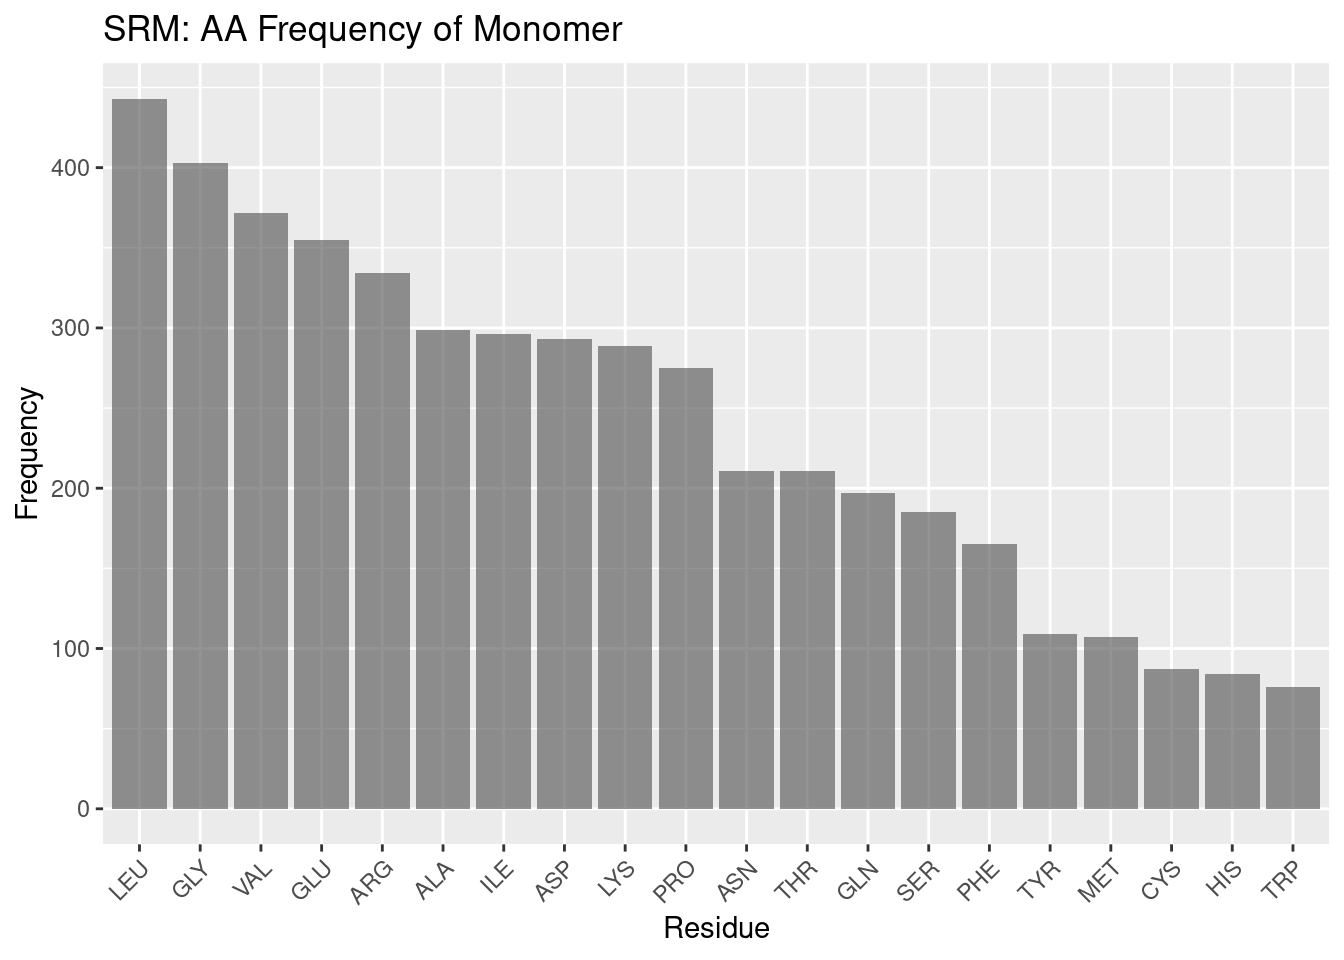
\includegraphics{_main_files/figure-latex/SRM-AAfreqAll-1.pdf}
\caption{\label{fig:SRM-AAfreqAll}SRM: AA Frequency of Monomer}
\end{figure}

Compared to the other heme molecules, siroheme's binding pocket amino acid frequencies are even more different than the background frequencies. Arginine is far and away the most frequent amino acid in the binding pocket - leucine is the most populous amino acid in the monomer overall, seeming to follow a trend amongst the hemoproteins examined so far. Again discussing the remainder of the frequencies of the monomer would be pure conjecture, but it is worthwhile to note that the pocket frequencies certainly appear unique against the background.

\hypertarget{distance-stuff}{%
\subsubsection{Distance stuff}\label{distance-stuff}}

Residues appear less uniformly distributed over distance for siroheme binding pockets when compared against the distribution for other heme molecules. Cysteine is the only residue that comes within 5A of siroheme; it is used to coordinate the iron in siroheme, so this result is expected. The lack of other residues being within 5A, differing from other heme molecules, suggests the many carboxyl and propionate groups on siroheme prevent, or preclude the need for closer interaction except for coordinating residues.

\begin{figure}
\centering
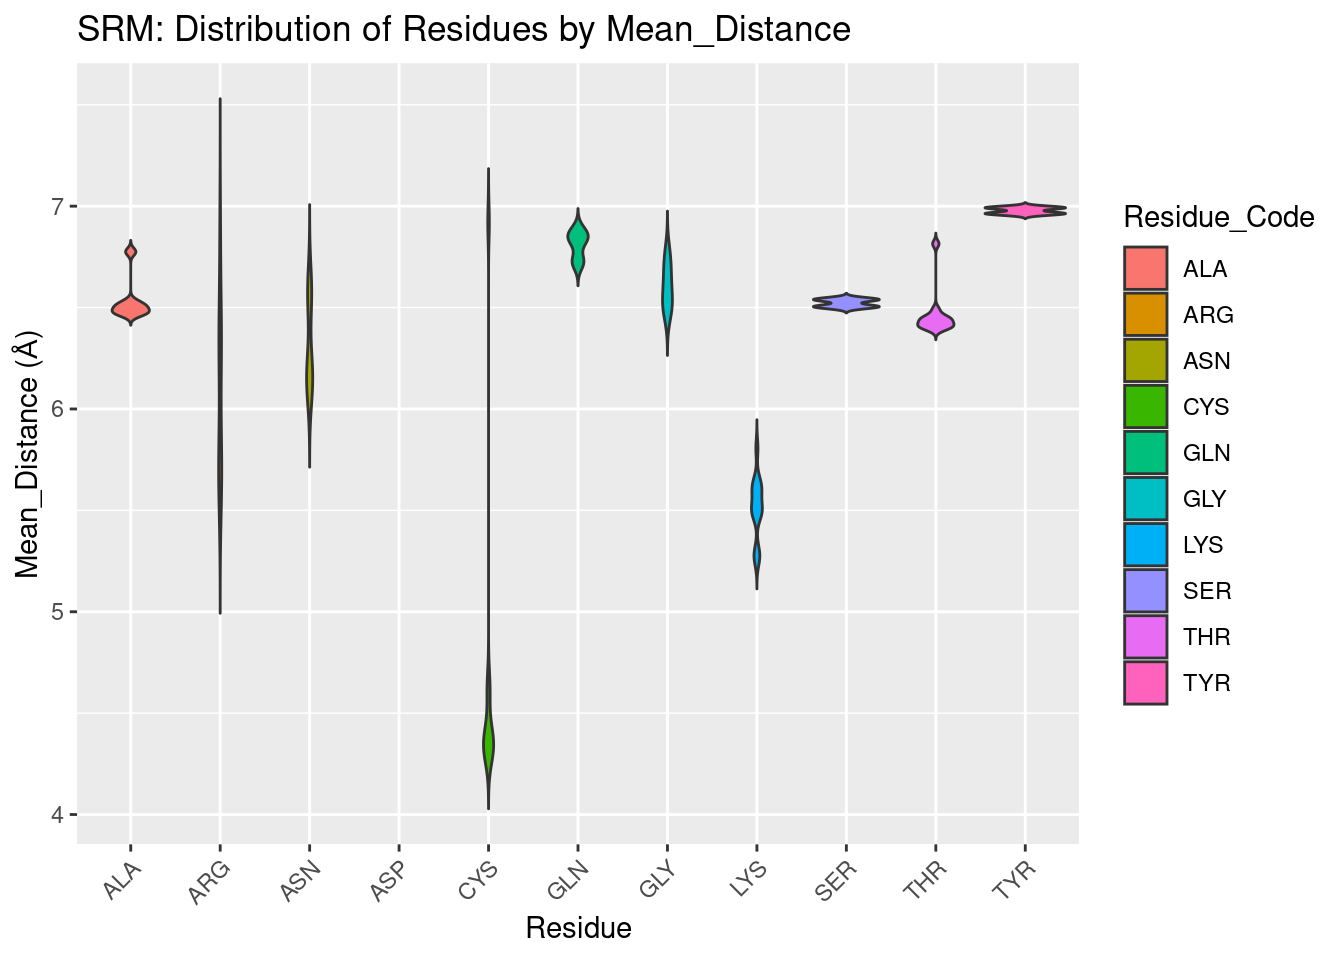
\includegraphics{_main_files/figure-latex/SRM-AAdist-1.pdf}
\caption{\label{fig:SRM-AAdist}SRM: AA Distances}
\end{figure}

\hypertarget{volume-discussion}{%
\section{Volume Discussion}\label{volume-discussion}}

Figures can be found in Appendix \ref{figs-vol}.

\textbf{worthwhile to add SD measures? 'x\% values fall within\ldots{}}
The utility of this result is somewhat dubious, at least within the context of this study. Volume results were rather spread out, with close agreement only found for heme-b. In general, volume for all heme molecules regardless of distance cutoff averaged about 1200 A³. This is somewhat contrived, and the result is not useful for elucidating the binding environment further; perhaps for other studies this result, or its lack of precision, may be informative.

\hypertarget{surface-areas}{%
\section{Surface Areas}\label{surface-areas}}

\hypertarget{surface-area-of-heme-molecules}{%
\subsection{Surface Area of Heme Molecules}\label{surface-area-of-heme-molecules}}

\textbf{Just going off solvent accessible, since that's really all that's of chemical importance. Can mention the excluded data is in the appendix}

Both solvent accessible and solvent excluded surface areas were calculated for heme molecules and binding pockets. The results are extremely similar and only solvent accesible surface area, a measure more practically interpreted into chemical phenonema, is discussed; figures and data for solvent excluded surface areas are available in Appendix (FIXME: insert reference)

\textbf{worth it to add SD etc? I think maybe, if time. Would leave raw data in appendix and add summary statistics in this section}

The solvent accessible surface area for all heme molecules themselves centers around values of 1000 A². This result is reasonable, given the similarity in size and structure of all heme molecules, in spite of the attached groups. Figures are shown below; extreme outliers have been removed from these figures but full data tables are available in (FIXME add appendix number). The outliers are likely artefacts of the method used to calculate surface area and potential conflicts with the method used to convert multimeric proteins to monomers. \textbf{worth to include this last statement?}

\hypertarget{surface-area-of-binding-pockets}{%
\section{Surface Area of Binding Pockets}\label{surface-area-of-binding-pockets}}

The surface area of binding pockets is more varied than the heme surface areas.

Heme-b and verdoheme, being highly similar molecules, with the same propionate groups, and one the derivative of the other, have quite similar surface areas, centering around 10,000-11,000 A². This is useful as a baseline to discuss the surface area of the binding pockets of the other two heme molecules below.

The surface area of the binding pocket of heme-c is considerably lower than that of heme-b and verdoheme. Its values center around 7500 A². Heme-c is bound covalently to the hemoprotein, forming thioether bonds with cysteine residues at two sites, excluding these sites from interacting with water molecules. \textbf{is this all that explains the reduction in SA? forgive my ignorance!}

The surface area of siroheme's binding pocket is far greater than that for other heme molecules - values center around 21000 A². Siroheme's extra groups do not appear to affect its own surface area, per above. However, it is effectively a very polar molecule and appropriately the binding pocket is highly saturated with very polar amino acids, as seen in the amino acid frequency analysis. The binding pocket is therefore completely different from the other heme molecules, and these populous, polar amino acids favorably interact with aqueous solvent, negating the need to bury any hydrophobic residues and reduce surface area.

\hypertarget{angular-data}{%
\section{Angular Data}\label{angular-data}}

**I think I'll just stick all of this in the appendix, including highlighting the clusters of data. Nothing can be discussed from it - it is interesting to note and perhaps I'll include some examples below very briefly, but otherwise, I don't know what value would be added to the report of ``verdoheme always has his interact with a planar angle of 116 degrees''

Figures can be found in \ref{figs-planarAll}

These data, for all ligands, except potentially for heme-c, largely serve to compare as noise for the next section. The planar angles of all residues, falling within the upper distance cutoff of 7A, are plotted.

In the notable exception of heme-c, Figure \textbf{FIXME: insert figure name} seems to suggest that GLU, MET and LYS have fairly specific planar angles with the ligand. Lysine is effectively the median of amino acid frequency for heme-c, methionine is even less frequent and glutamine is the least frequent amino acid. For the latter two amino acids their tight range of planar angles is therefore likely an artefact of a small sample size of amino acids. However, for lysine the tight range of angles may be significant; this is dicussed further below.

\hypertarget{planar-angles-of-closest-residues}{%
\section{Planar Angles of Closest Residues}\label{planar-angles-of-closest-residues}}

Figures can be found in \ref{figs-planarClosest}

Here, the three closest residues to the ligand in each PDDB and their planar angle to the ligand are plotted. Data are summarized below, and discussed below.

HEM has a fairly inconclusive set of data for this measure. GLU and GLN nearby HEM do appear to fall within a tight range, though, of approximately 75 degrees and 80 degrees respectively.

The data for residues nearby HEC diverge from what is found for all residues around HEC. The most agreement is found for ILE and LYS, with angles concentrated about 50 degrees and 75 degrees, respectively.

\hypertarget{all-ca-cb-fe-angles}{%
\section{All CA-CB-Fe Angles}\label{all-ca-cb-fe-angles}}

Figures can be found in \ref{figs-cabAll}

\hypertarget{ca-cb-fe-angles-of-closest-residues}{%
\section{CA-CB-Fe Angles of Closest Residues}\label{ca-cb-fe-angles-of-closest-residues}}

Figures can be found in \ref{figs-cabClosest}

\hypertarget{limitations-of-the-study}{%
\section{Limitations of the Study}\label{limitations-of-the-study}}

Limited sample size

Limited experimental data to reference to verify

NO experimental data in this study to verify, all theoretical

Only one software package/few algorithms used to calculate all these properties. Others were evaluated but none are compared w.

Algorithms may introduce bias based on how they work e.g.~all the bubbles

Arbitrary selection of parameters; some based on rule of thumb or visual evaluation but all or almost all arbitrary

Unknown if the qualities measured are truly the most critical for the heme binding. Some papers suggest other properties may also be important but cannot be calculated, at least right now, e.g.~ionic bonding strength etc.

Visual examination itself to OK the parameters/algorithms can introduce bias

\adjustmtc
\markboth{Methods}{}

\hypertarget{conclusion}{%
\chapter{Conclusion}\label{conclusion}}

A knowledge gap in the binding environment for heme exists in the present literature. A high-throughput framework employing UCSF Chimera was constructed to process diverse sets of hemoproteins and output information about their binding pockets: amino acid frequencies and distances from heme, volume, surface area, angles. Data was gathered and predicted from representative and varied datasets for heme-b, heme-c, verdoheme, and siroheme, and their respective hemoproteins. R was used to analyze all data.

The results of this study are limited by the small sample size, but suggest that binding pockets for hemoproteins have some requirements for binding that may be overlooked, e.g.~a high population of nonpolar amino acids for heme-b, heme-c, and verdoheme which may provide much of the interactions necessary to bind heme; in the case of siroheme there is a preponderance of polar amino acids. In either case both polar and nonpolar amino acids appear in force, suggesting both types of interactions are important to bind heme. Volumes are within reason. Surface area results reinforce, demonstrate the significance of the amino acid frequency results and show pockets have lesser or greater surface area depending on the involvemnt of covalent bonds or preferences for polar amino acids. Angular data, while not able to be interpreted into useful results, is produced and a framework provided for future study.

These results may be useful in the rational design of hemoproteins in the future, with the importance of nonpolar interactions in particular likely of great interest. The framework constructed can be applied to any list of PDBs and their respective ligands, thereby facilitating similar research for other proteins.

\startappendices

\hypertarget{a-figures}{%
\chapter{Figures}\label{a-figures}}

\hypertarget{figs-aaFreqOverlaid}{%
\section{AA Frequency}\label{figs-aaFreqOverlaid}}

\begin{figure}
\centering
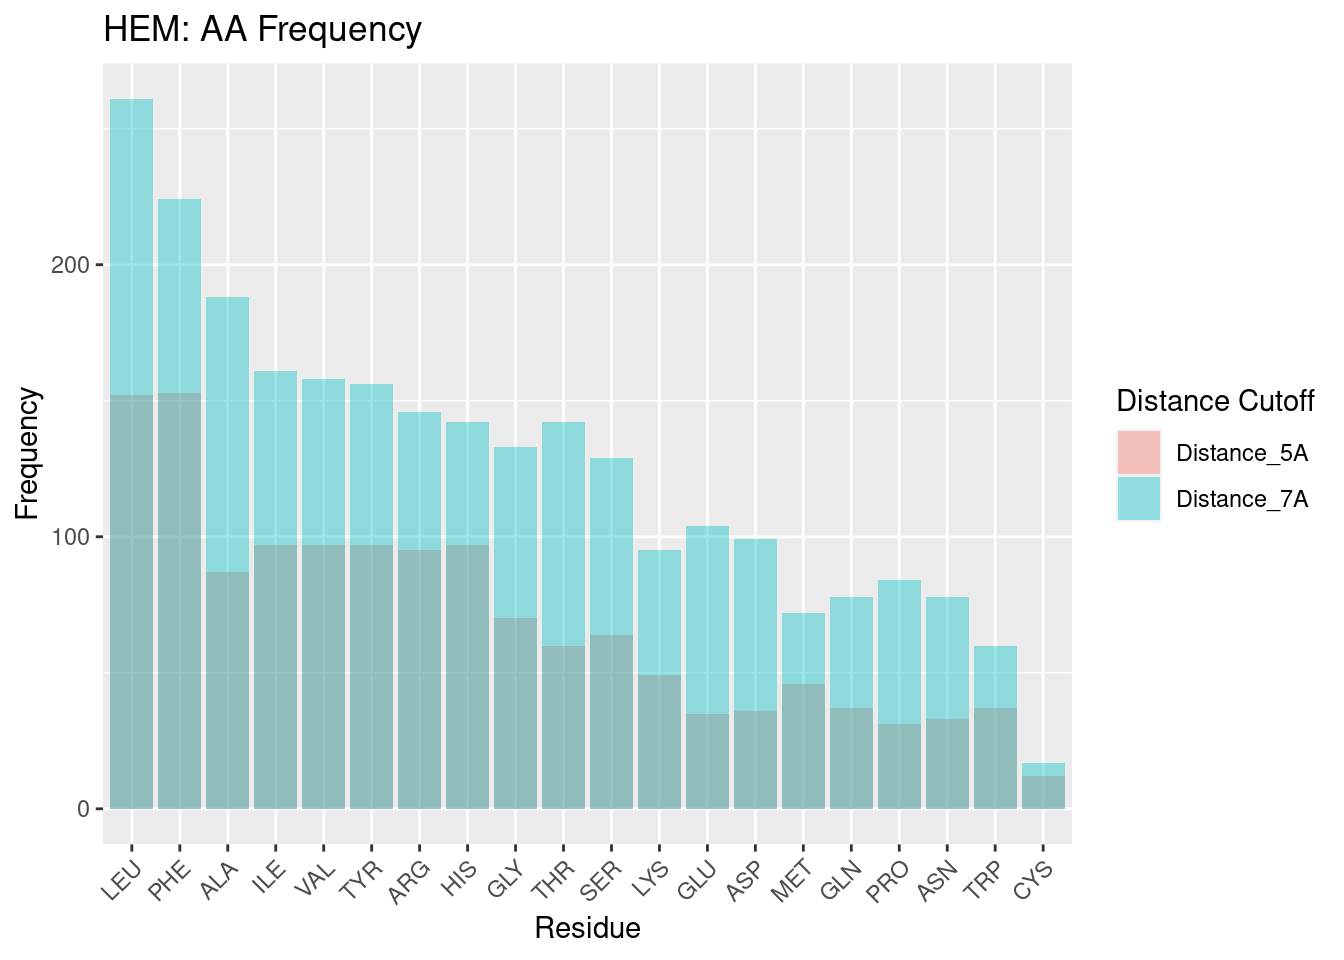
\includegraphics{_main_files/figure-latex/HEM-AAfreqOverlaid-1.pdf}
\caption{\label{fig:HEM-AAfreqOverlaid}HEM: AA Frequency}
\end{figure}

\begin{figure}
\centering
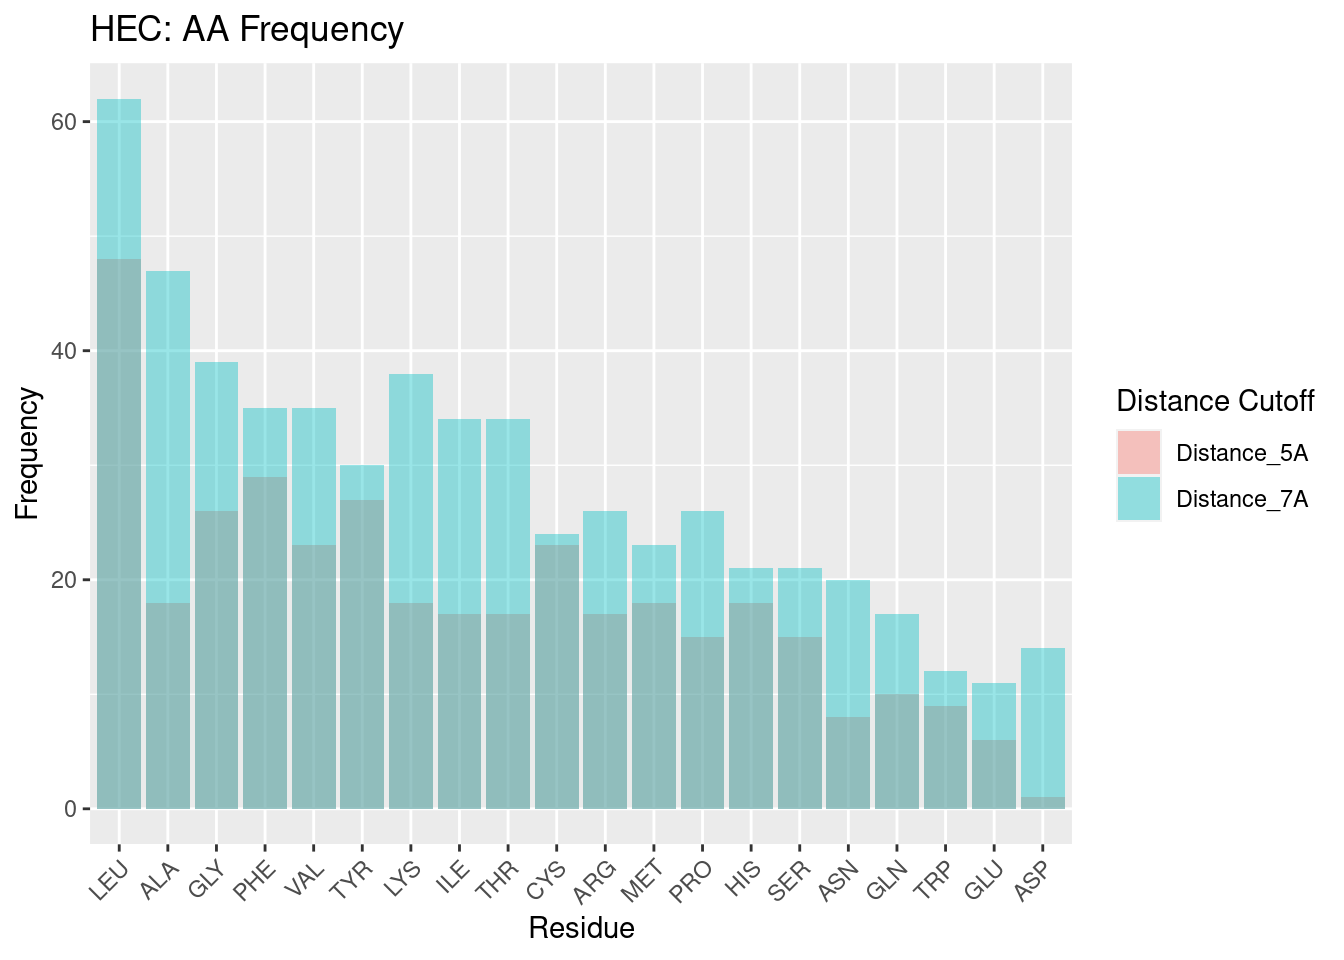
\includegraphics{_main_files/figure-latex/HEC-AAfreqOverlaid-1.pdf}
\caption{\label{fig:HEC-AAfreqOverlaid}HEC: AA Frequency}
\end{figure}

\begin{figure}
\centering
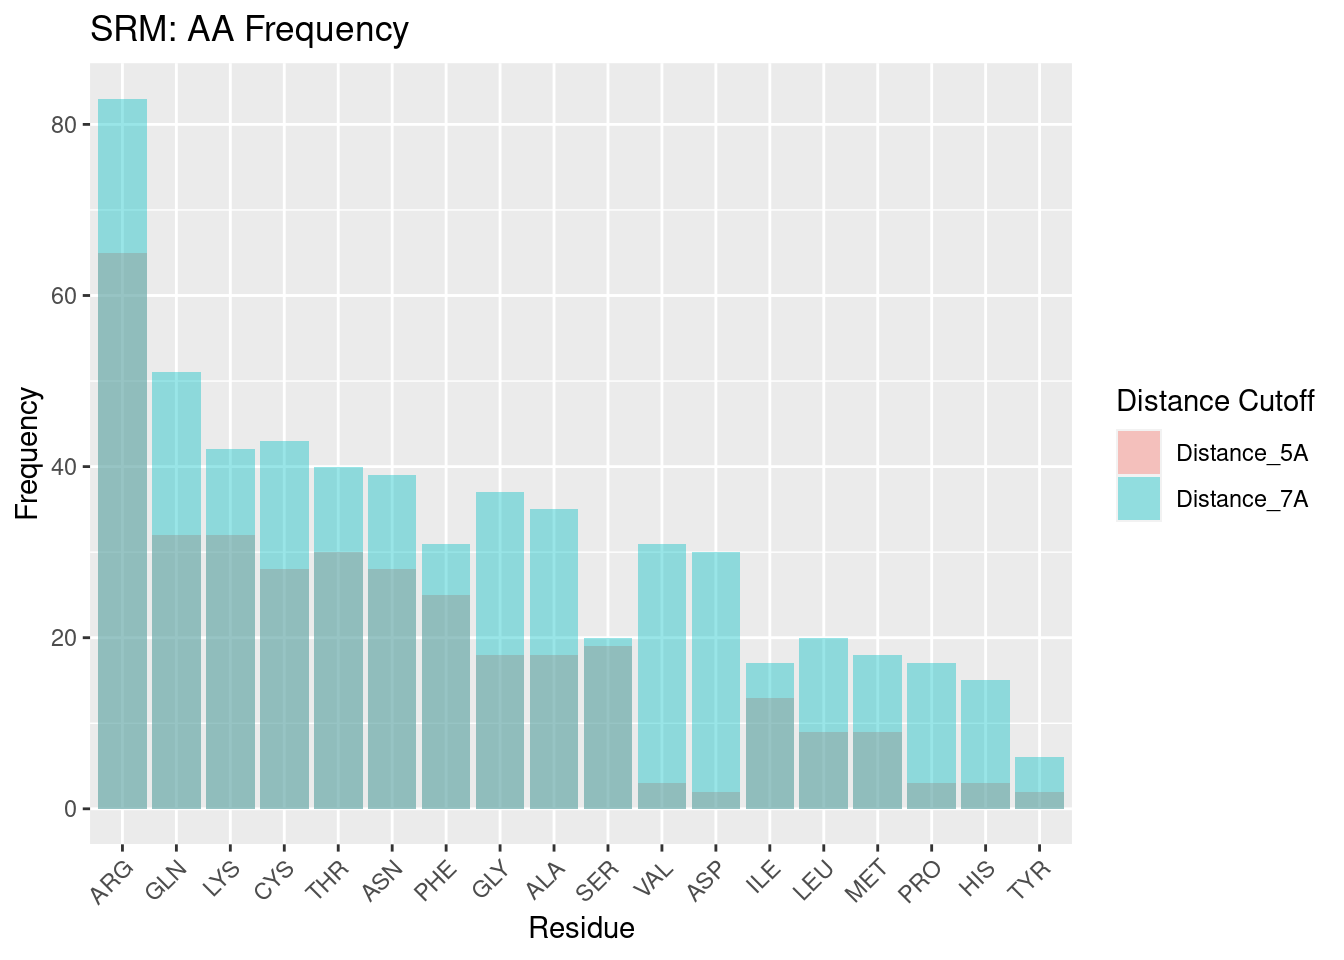
\includegraphics{_main_files/figure-latex/SRM-AAfreqOverlaid-1.pdf}
\caption{\label{fig:SRM-AAfreqOverlaid}SRM: AA Frequency}
\end{figure}

\begin{figure}
\centering
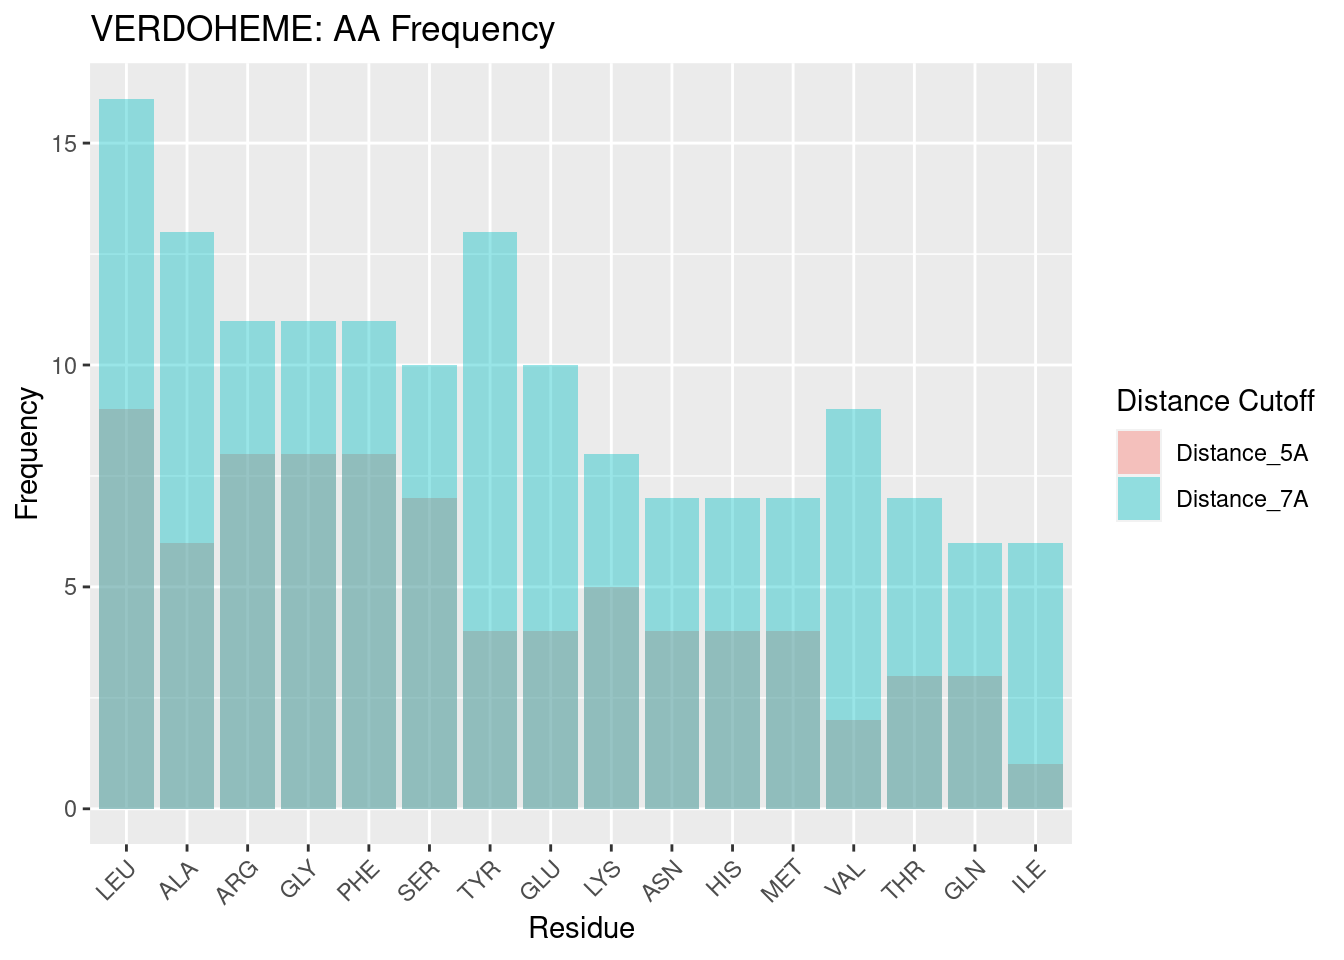
\includegraphics{_main_files/figure-latex/VERDOHEME-AAfreqOverlaid-1.pdf}
\caption{\label{fig:VERDOHEME-AAfreqOverlaid}VERDOHEME: AA Frequency}
\end{figure}

\hypertarget{figs-vol}{%
\section{Volume}\label{figs-vol}}

\begin{figure}
\centering
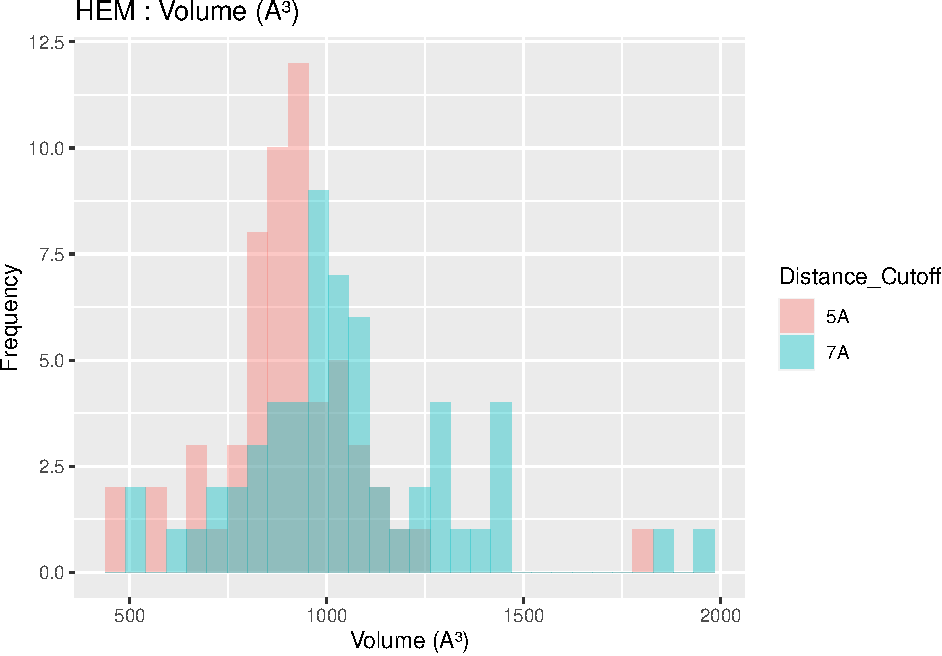
\includegraphics{_main_files/figure-latex/HEM-Volume-1.pdf}
\caption{\label{fig:HEM-Volume}HEM: Volume}
\end{figure}

\begin{figure}
\centering
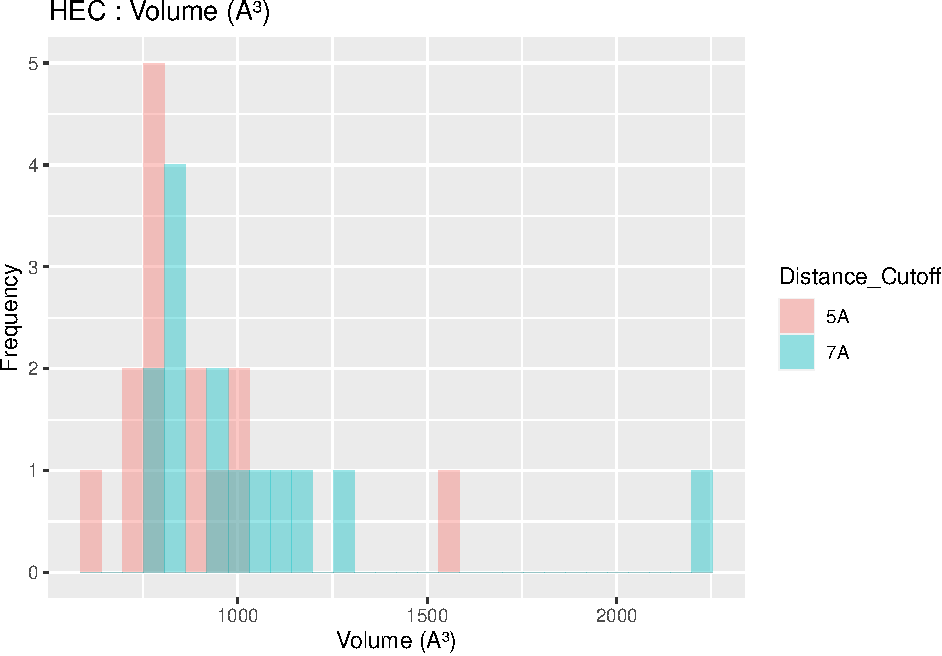
\includegraphics{_main_files/figure-latex/HEC-Volume-1.pdf}
\caption{\label{fig:HEC-Volume}HEC: Volume}
\end{figure}

\begin{figure}
\centering
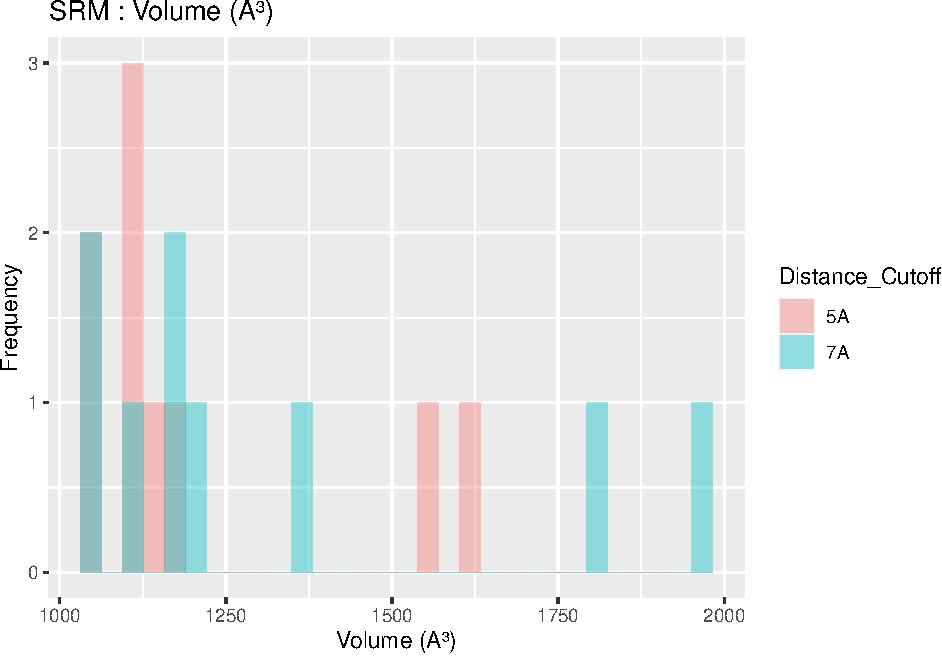
\includegraphics{_main_files/figure-latex/SRM-Volume-1.pdf}
\caption{\label{fig:SRM-Volume}SRM: Volume}
\end{figure}

\begin{figure}
\centering
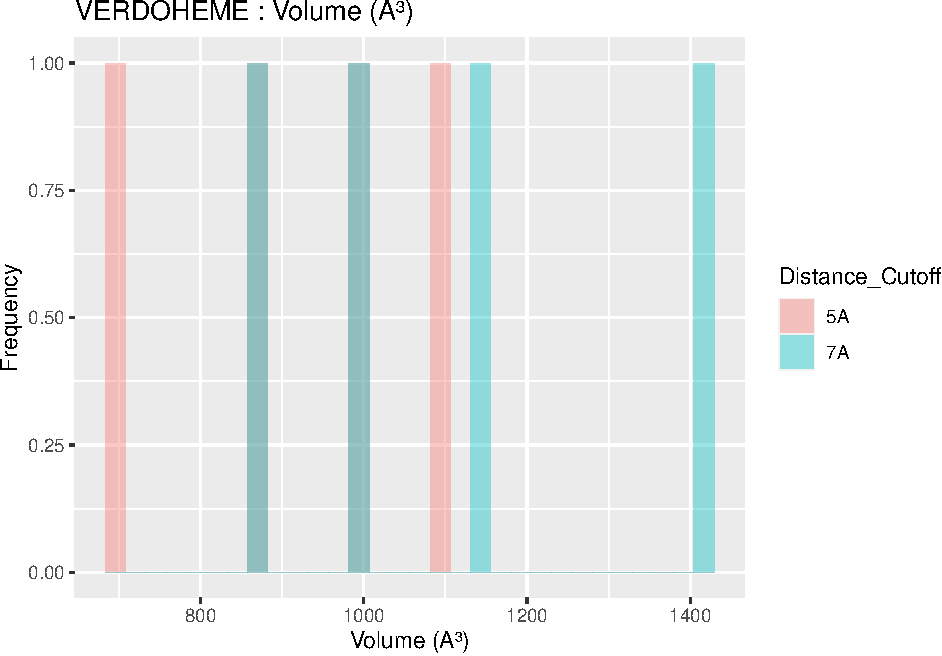
\includegraphics{_main_files/figure-latex/VERDOHEME-Volume-1.pdf}
\caption{\label{fig:VERDOHEME-Volume}VERDOHEME: Volume}
\end{figure}

\hypertarget{figs-ligExcSA}{%
\section{Ligand Excluded Surface Area}\label{figs-ligExcSA}}

\begin{figure}
\centering
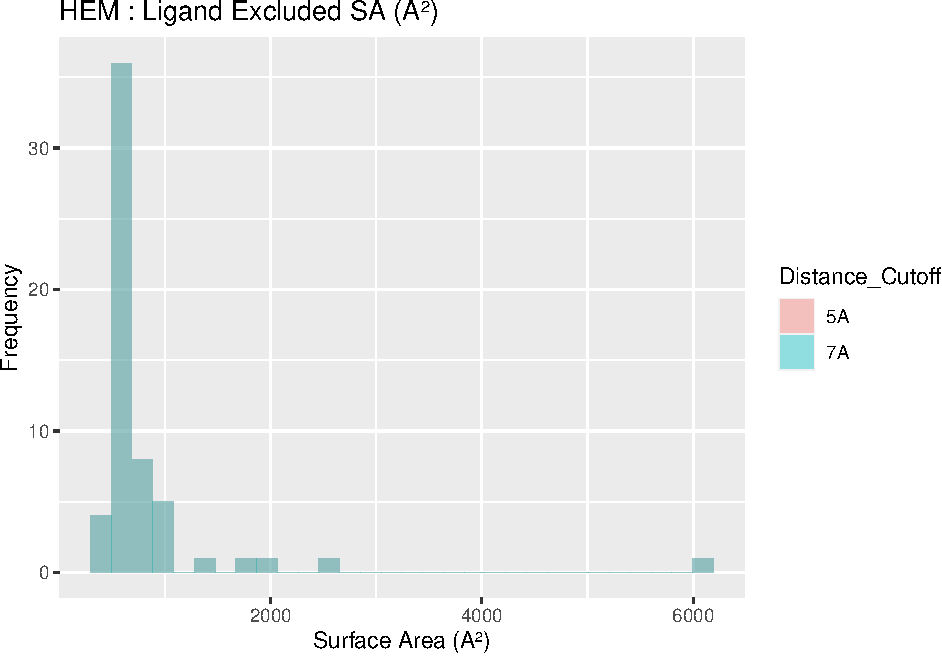
\includegraphics{_main_files/figure-latex/HEM-Ligand-ExcludedSA-1.pdf}
\caption{\label{fig:HEM-Ligand-ExcludedSA}HEM: Ligand Excluded Suface Area}
\end{figure}

\begin{figure}
\centering
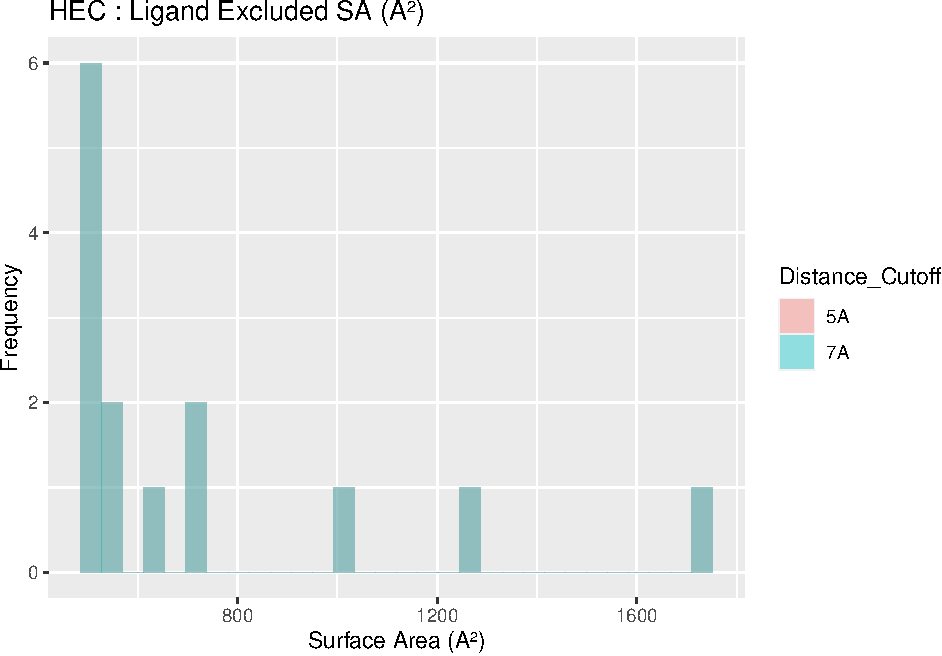
\includegraphics{_main_files/figure-latex/HEC-Ligand-ExcludedSA-1.pdf}
\caption{\label{fig:HEC-Ligand-ExcludedSA}HEC: Ligand Excluded Suface Area}
\end{figure}

\begin{figure}
\centering
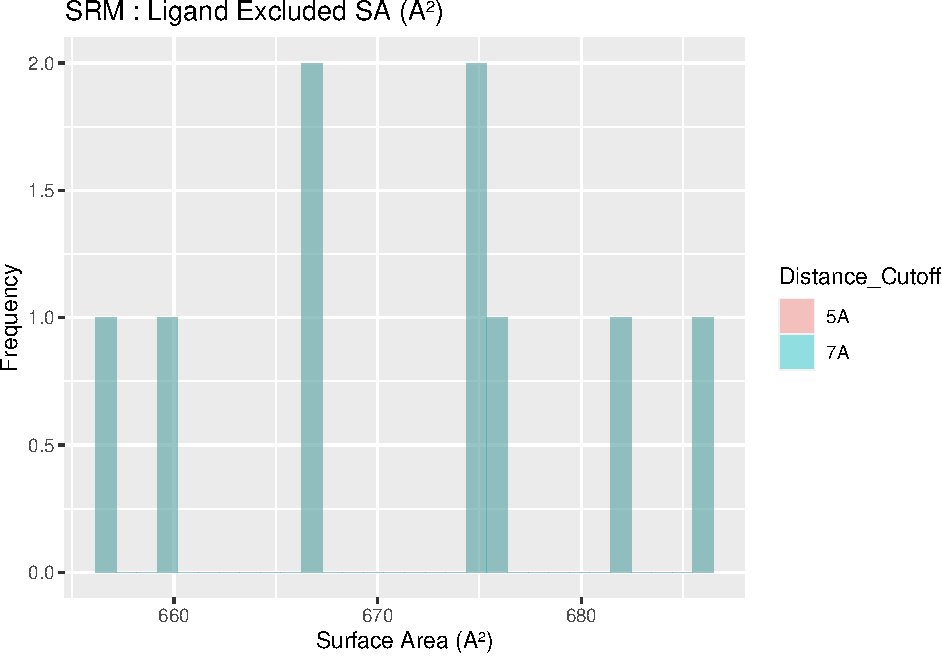
\includegraphics{_main_files/figure-latex/SRM-Ligand-ExcludedSA-1.pdf}
\caption{\label{fig:SRM-Ligand-ExcludedSA}SRM: Ligand Excluded Suface Area}
\end{figure}

\begin{figure}
\centering
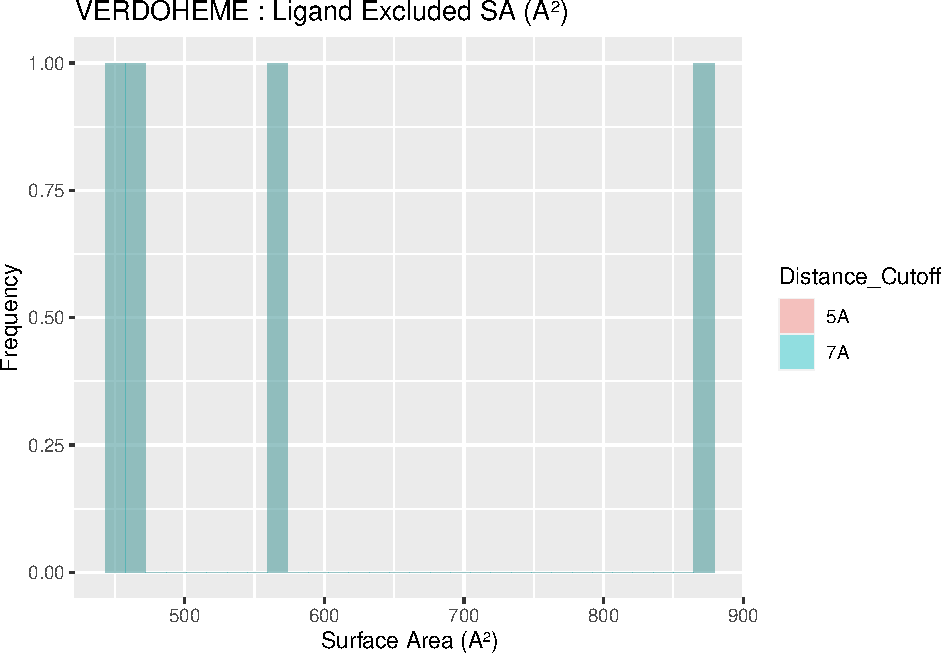
\includegraphics{_main_files/figure-latex/VERDOHEME-Ligand-ExcludedSA-1.pdf}
\caption{\label{fig:VERDOHEME-Ligand-ExcludedSA}VERDOHEME: Ligand Excluded Suface Area}
\end{figure}

\hypertarget{figs-ligAccSA}{%
\section{Ligand Accessible Surface Area}\label{figs-ligAccSA}}

\begin{figure}
\centering
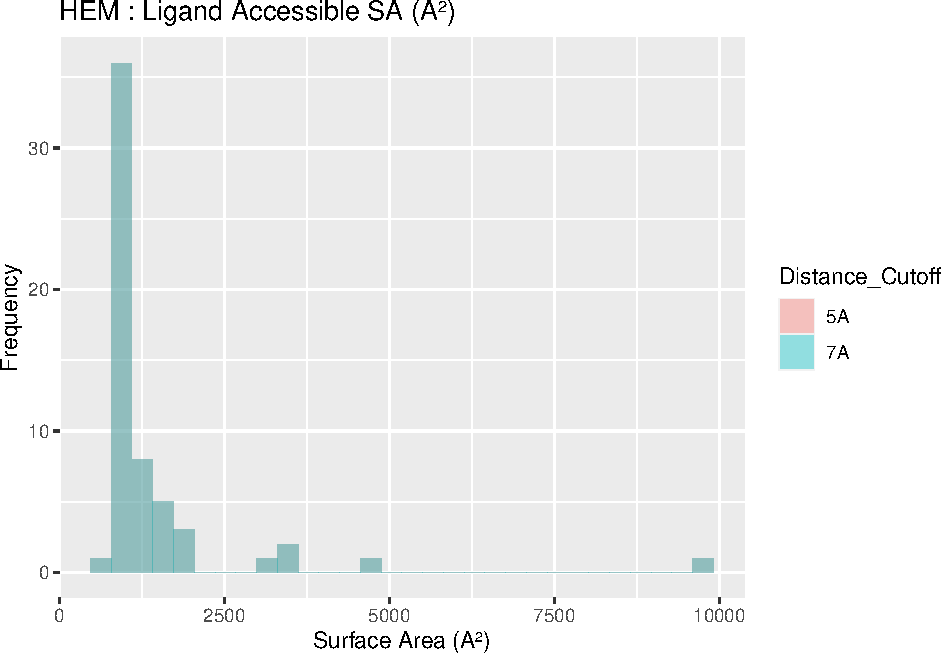
\includegraphics{_main_files/figure-latex/HEM-Ligand-AccessibleSA-1.pdf}
\caption{\label{fig:HEM-Ligand-AccessibleSA}HEM: Ligand Accessible Surface Area}
\end{figure}

\begin{figure}
\centering
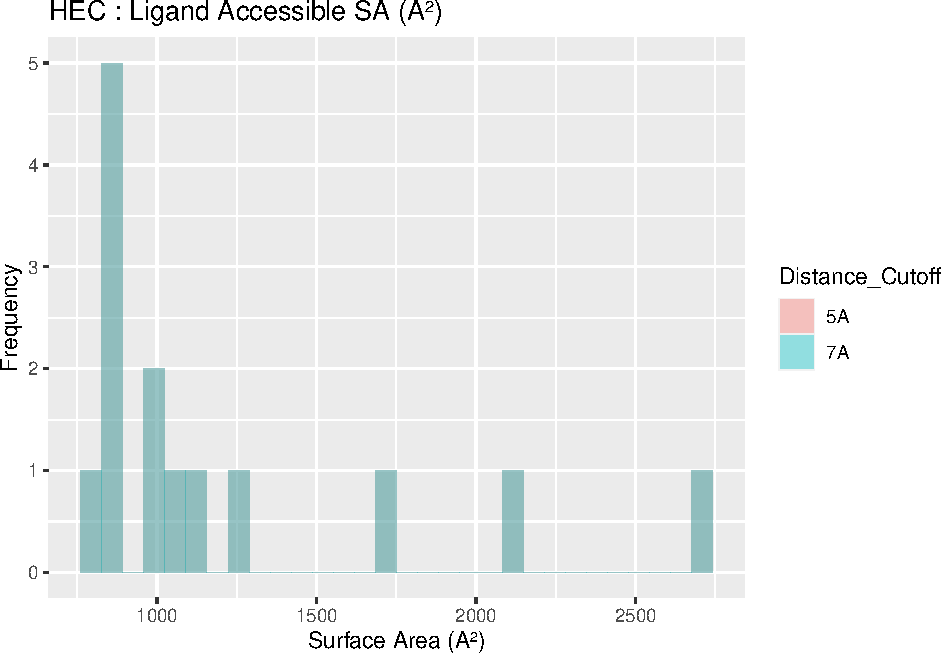
\includegraphics{_main_files/figure-latex/HEC-Ligand-AccessibleSA-1.pdf}
\caption{\label{fig:HEC-Ligand-AccessibleSA}HEC: Ligand Accessible Surface Area}
\end{figure}

\begin{figure}
\centering
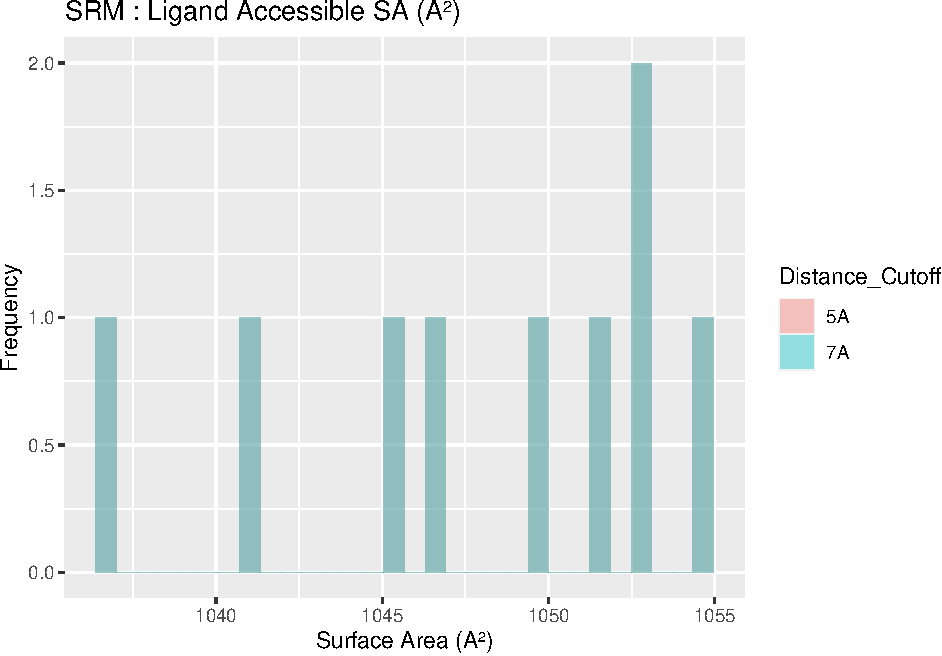
\includegraphics{_main_files/figure-latex/SRM-Ligand-AccessibleSA-1.pdf}
\caption{\label{fig:SRM-Ligand-AccessibleSA}SRM: Ligand Accessible Surface Area}
\end{figure}

\begin{figure}
\centering
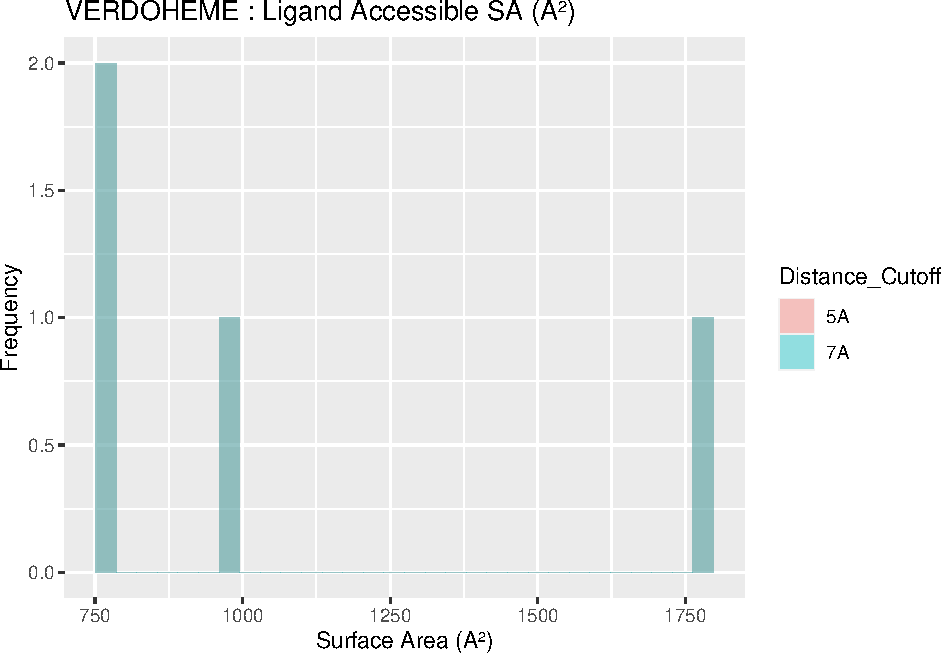
\includegraphics{_main_files/figure-latex/VERDOHEME-Ligand-AccessibleSA-1.pdf}
\caption{\label{fig:VERDOHEME-Ligand-AccessibleSA}VERDOHEME: Ligand Accessible Surface Area}
\end{figure}

\hypertarget{figs-pocketExcSA}{%
\section{Pocket Excluded Surface Area}\label{figs-pocketExcSA}}

\begin{figure}
\centering
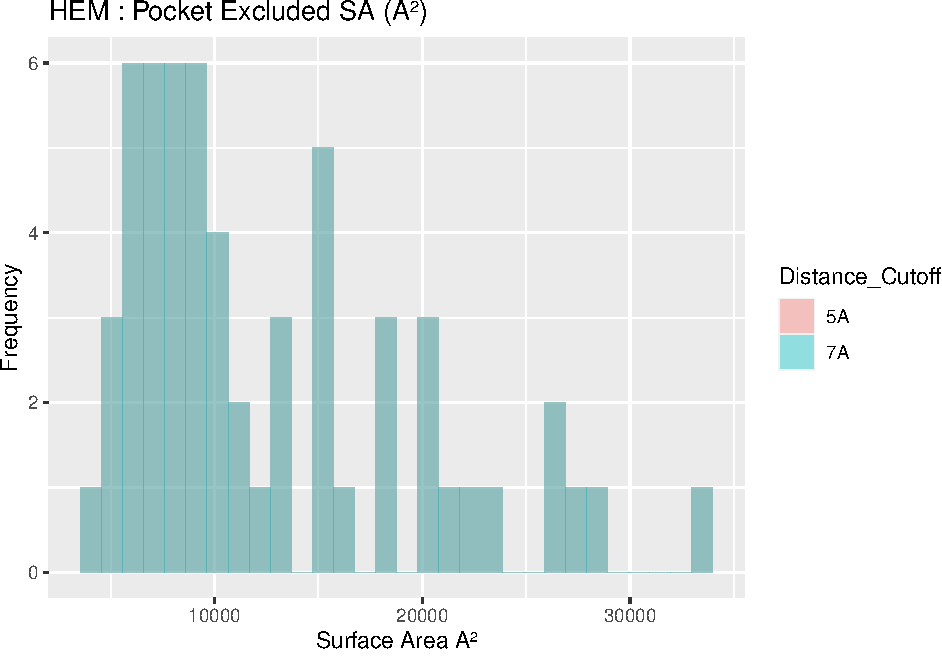
\includegraphics{_main_files/figure-latex/HEM-Pocket-ExcludedSA-1.pdf}
\caption{\label{fig:HEM-Pocket-ExcludedSA}HEM: Pocket Excluded Surface Area}
\end{figure}

\begin{figure}
\centering
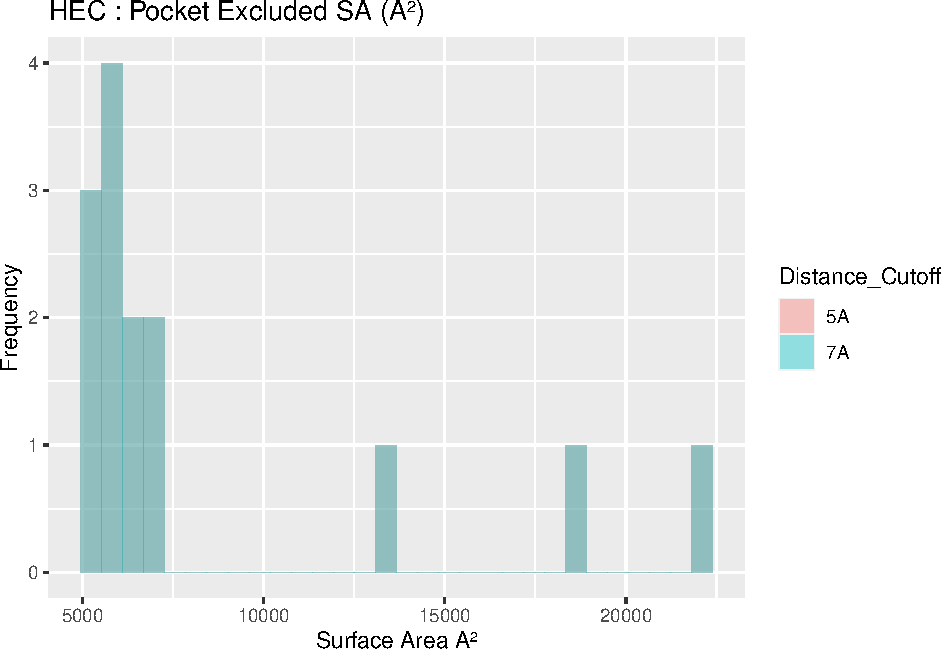
\includegraphics{_main_files/figure-latex/HEC-Pocket-ExcludedSA-1.pdf}
\caption{\label{fig:HEC-Pocket-ExcludedSA}HEC: Pocket Excluded Surface Area}
\end{figure}

\begin{figure}
\centering
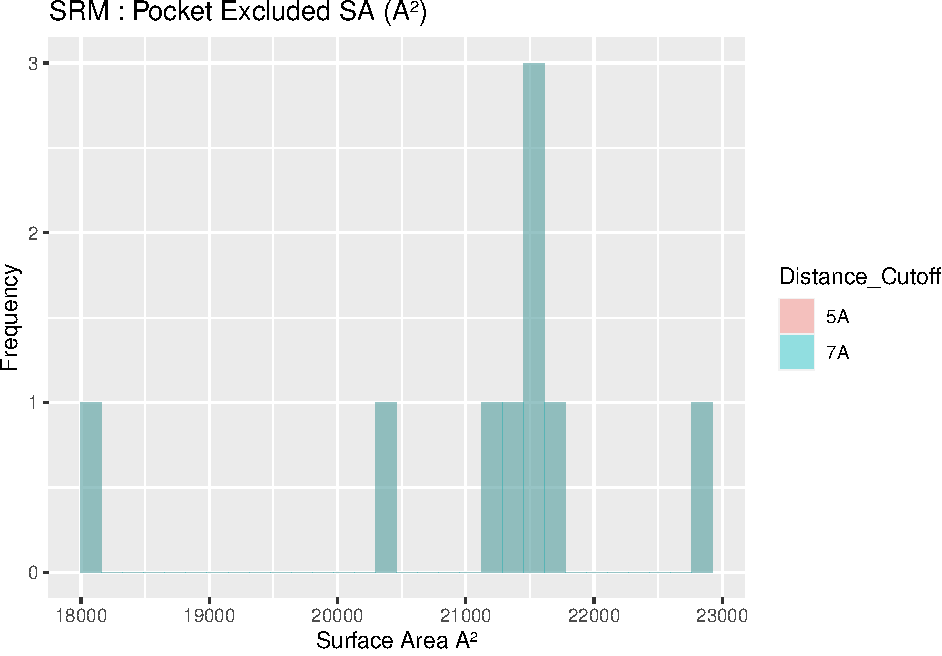
\includegraphics{_main_files/figure-latex/SRM-Pocket-ExcludedSA-1.pdf}
\caption{\label{fig:SRM-Pocket-ExcludedSA}SRM: Pocket Excluded Surface Area}
\end{figure}

\begin{figure}
\centering
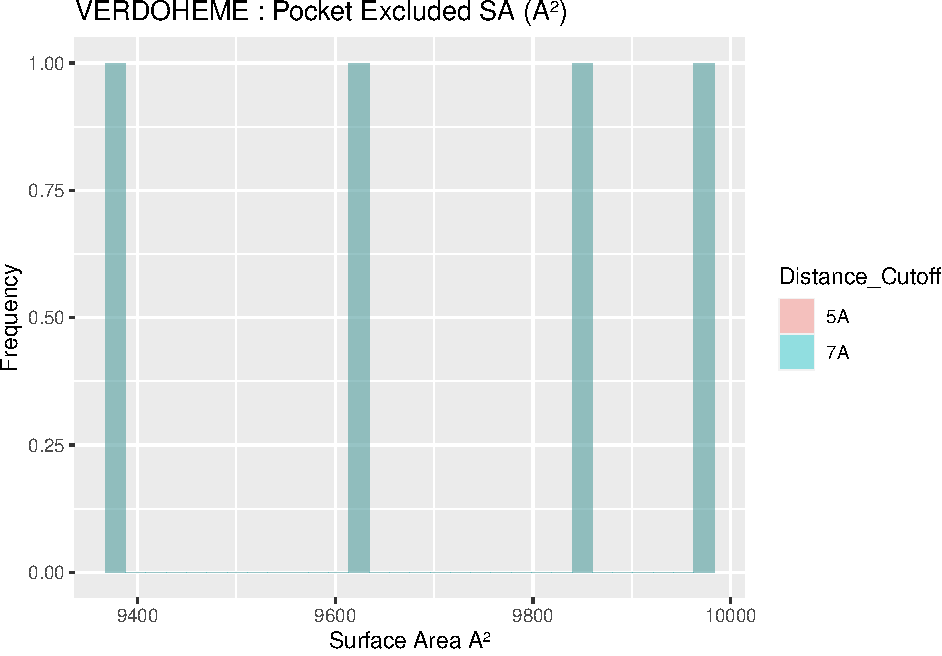
\includegraphics{_main_files/figure-latex/VERDOHEME-Pocket-ExcludedSA-1.pdf}
\caption{\label{fig:VERDOHEME-Pocket-ExcludedSA}VERDOHEME: Pocket Excluded Surface Area}
\end{figure}

\hypertarget{figs-pocketAccSA}{%
\section{Pocket Accessible Surface Area}\label{figs-pocketAccSA}}

\begin{figure}
\centering
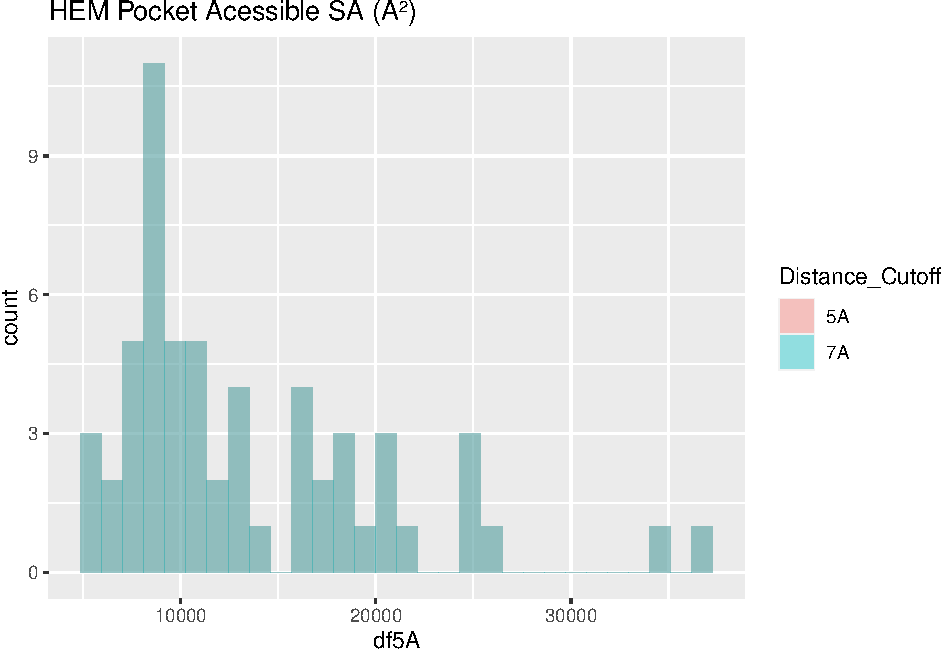
\includegraphics{_main_files/figure-latex/HEM-Pocket-AccessibleSA-1.pdf}
\caption{\label{fig:HEM-Pocket-AccessibleSA}HEM: Pocket Accessible Surface Area}
\end{figure}

\begin{figure}
\centering
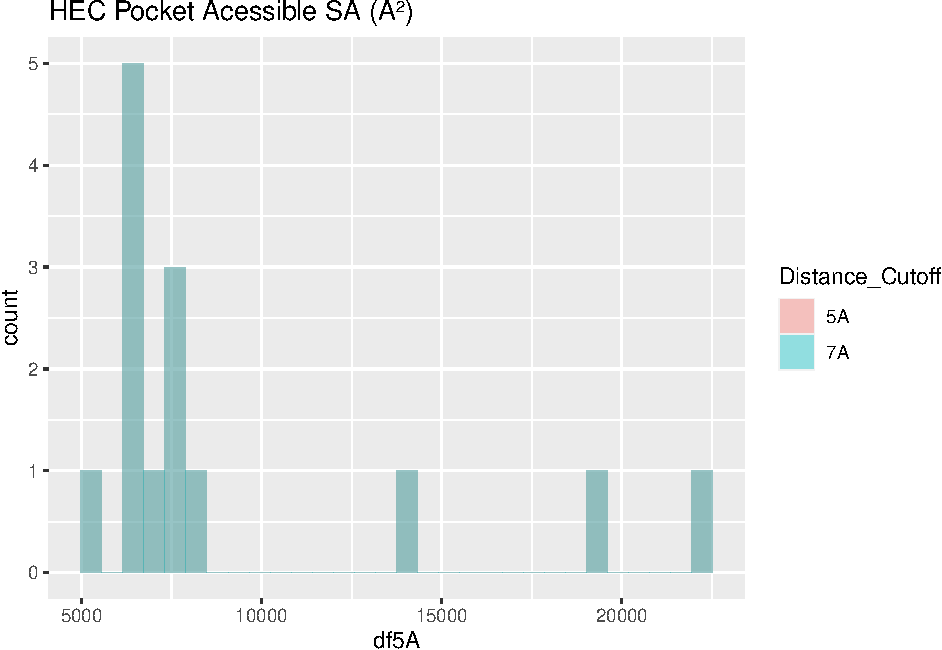
\includegraphics{_main_files/figure-latex/HEC-Pocket-AccessibleSA-1.pdf}
\caption{\label{fig:HEC-Pocket-AccessibleSA}HEC: Pocket Accessible Surface Area}
\end{figure}

\begin{figure}
\centering
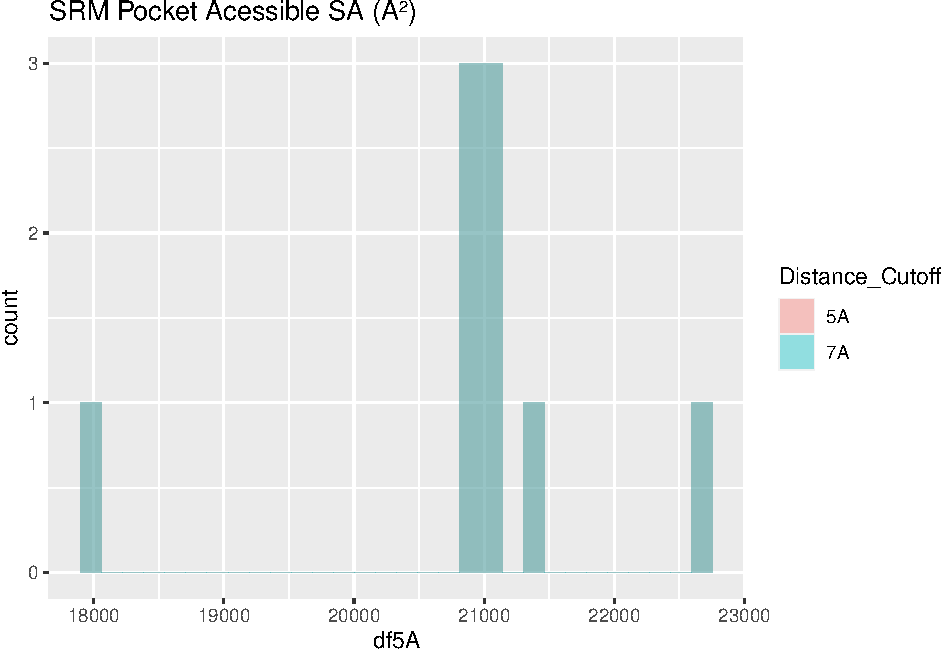
\includegraphics{_main_files/figure-latex/SRM-Pocket-AccessibleSA-1.pdf}
\caption{\label{fig:SRM-Pocket-AccessibleSA}SRM: Pocket Accessible Surface Area}
\end{figure}

\begin{figure}
\centering
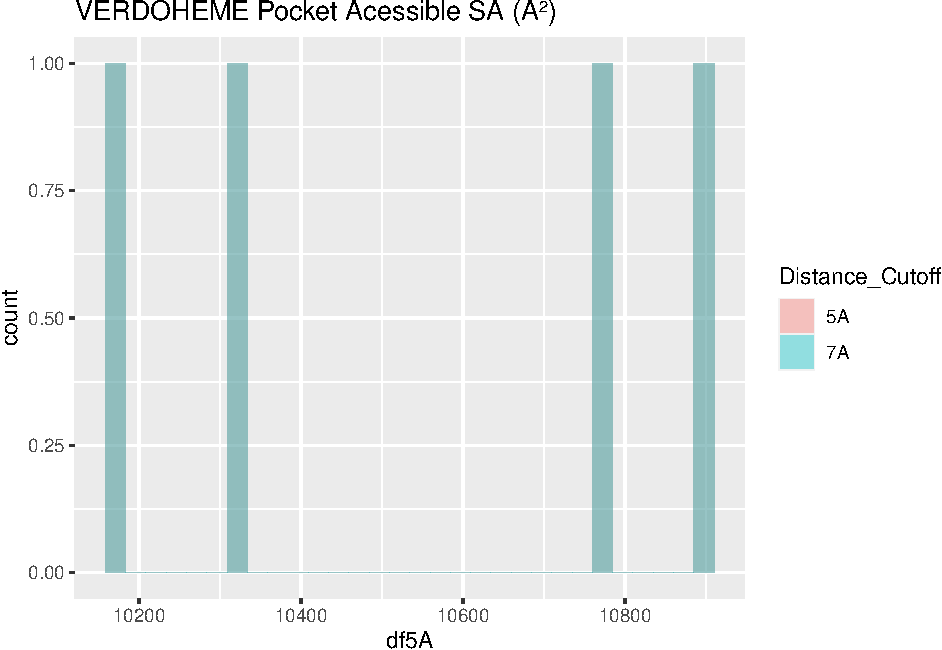
\includegraphics{_main_files/figure-latex/VERDOHEME-Pocket-AccessibleSA-1.pdf}
\caption{\label{fig:VERDOHEME-Pocket-AccessibleSA}VERDOHEME: Pocket Accessible Surface Area}
\end{figure}

\hypertarget{figs-planarAll}{%
\section{All Planar Angles}\label{figs-planarAll}}

\begin{figure}
\centering
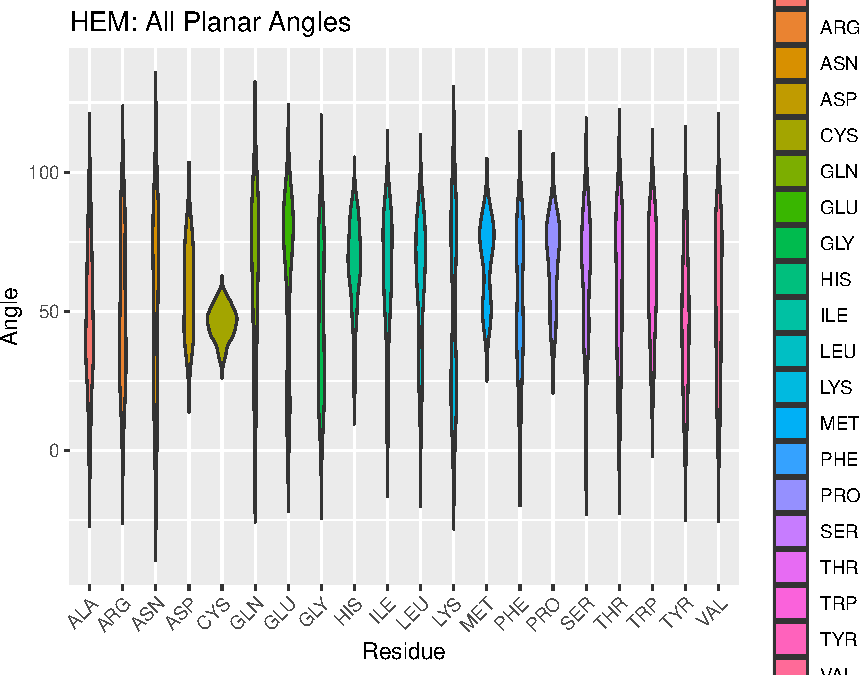
\includegraphics{_main_files/figure-latex/HEM-planarAll-1.pdf}
\caption{\label{fig:HEM-planarAll}HEM: All Planar Angles}
\end{figure}

\begin{figure}
\centering
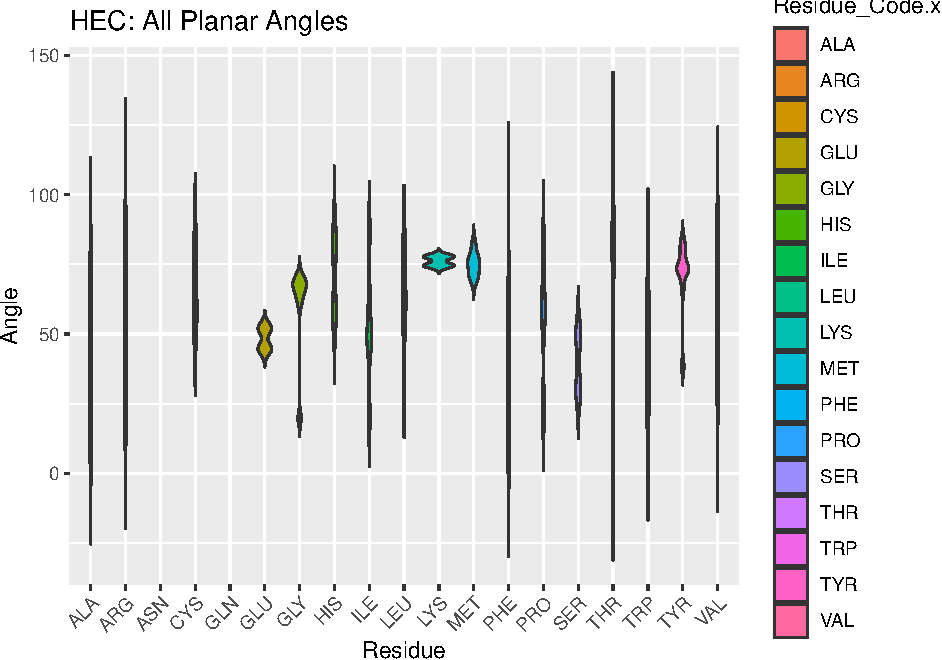
\includegraphics{_main_files/figure-latex/HEC-planarAll-1.pdf}
\caption{\label{fig:HEC-planarAll}HEC: All Planar Angles}
\end{figure}

\begin{figure}
\centering
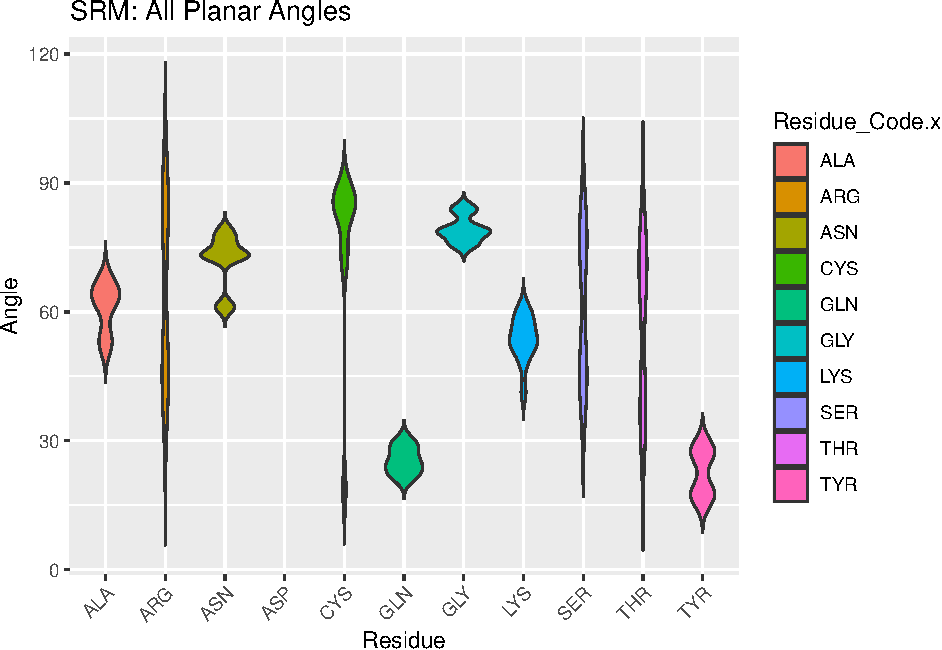
\includegraphics{_main_files/figure-latex/SRM-planarAll-1.pdf}
\caption{\label{fig:SRM-planarAll}SRM: All Planar Angles}
\end{figure}

\begin{figure}
\centering
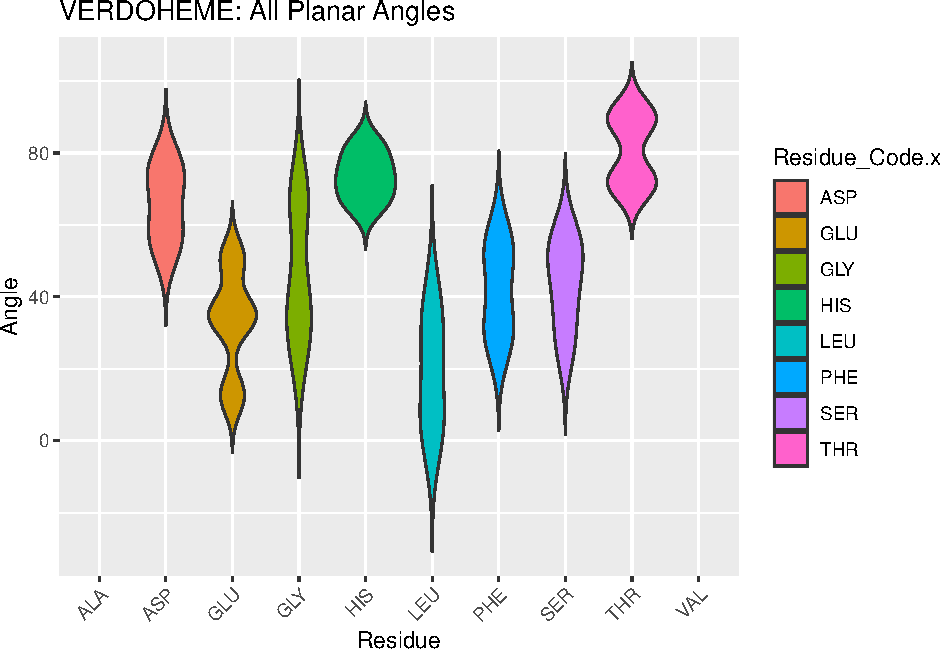
\includegraphics{_main_files/figure-latex/VERDOHEME-planarAll-1.pdf}
\caption{\label{fig:VERDOHEME-planarAll}VERDOHEME: All Planar Angles}
\end{figure}

\hypertarget{figs-planarClosest}{%
\section{Planar Angles of Closest Residues}\label{figs-planarClosest}}

\begin{figure}
\centering
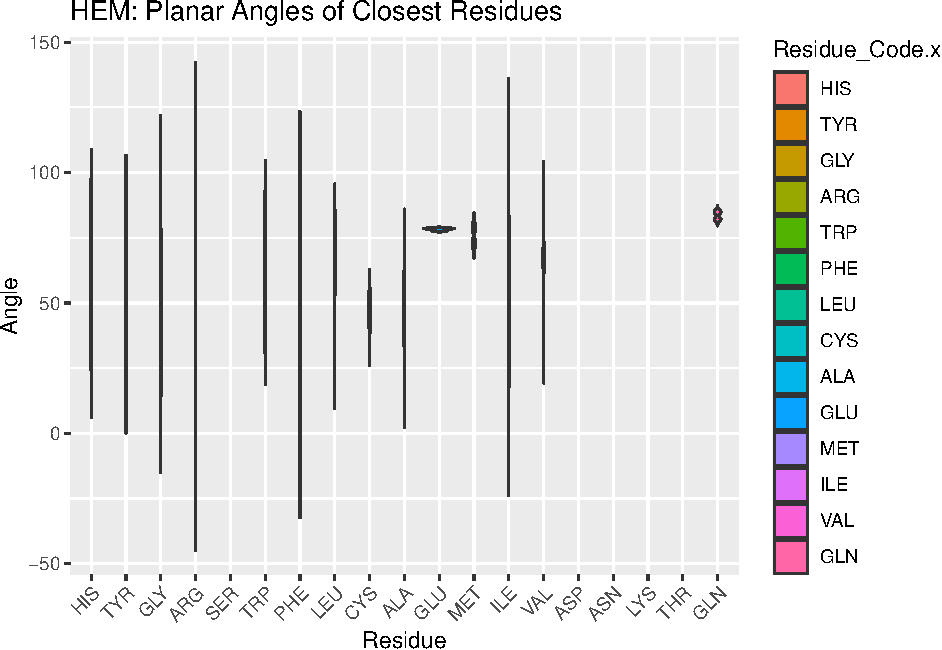
\includegraphics{_main_files/figure-latex/HEM-planarClosest-1.pdf}
\caption{\label{fig:HEM-planarClosest}HEM: Planar Angles of Closest Residues}
\end{figure}

\begin{figure}
\centering
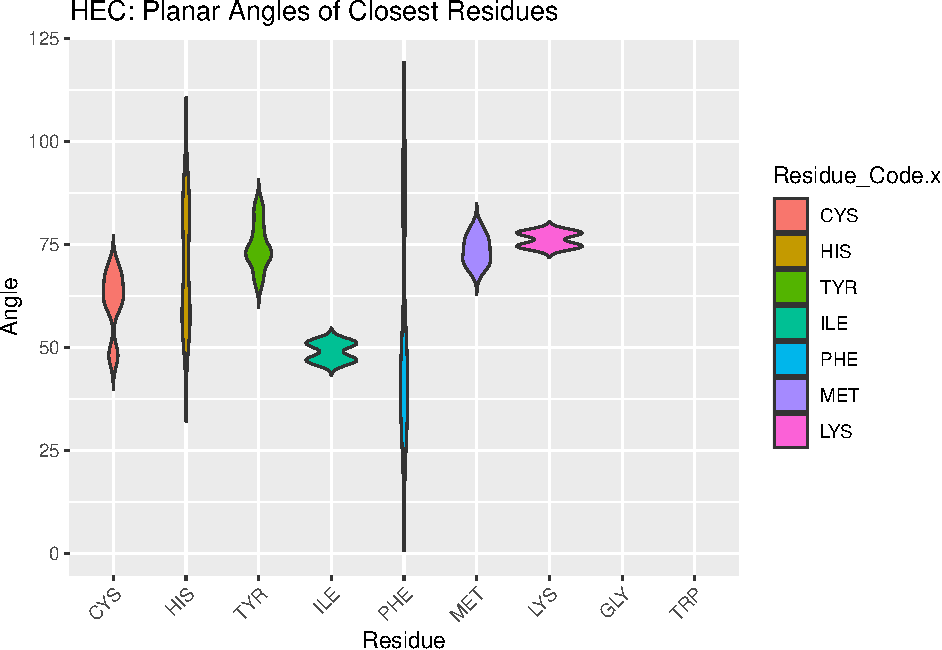
\includegraphics{_main_files/figure-latex/HEC-planarClosest-1.pdf}
\caption{\label{fig:HEC-planarClosest}HEC: Planar Angles of Closest Residues}
\end{figure}

\begin{figure}
\centering
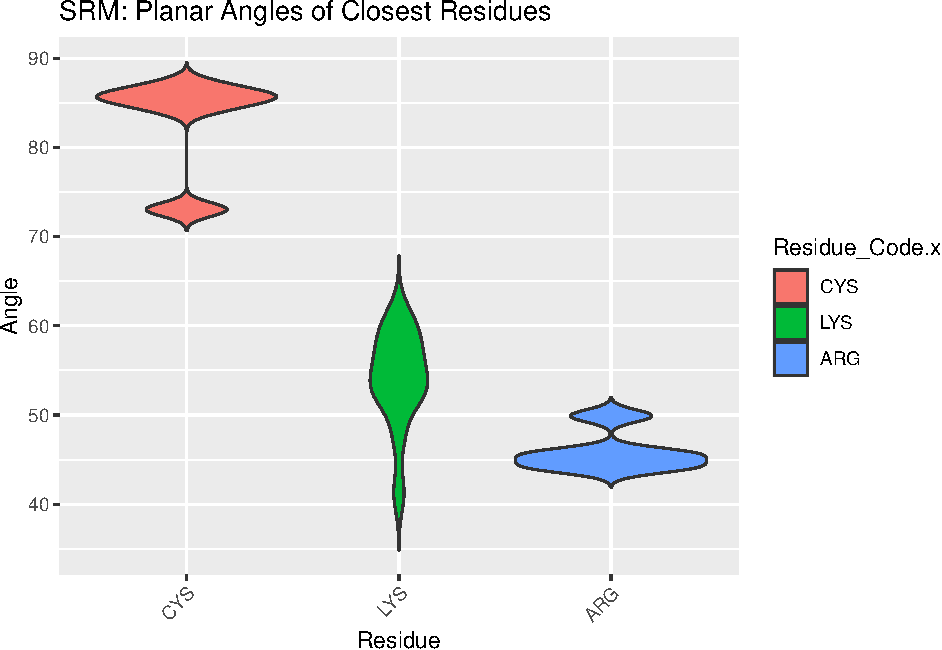
\includegraphics{_main_files/figure-latex/SRM-planarClosest-1.pdf}
\caption{\label{fig:SRM-planarClosest}SRM: Planar Angles of Closest Residues}
\end{figure}

\begin{figure}
\centering
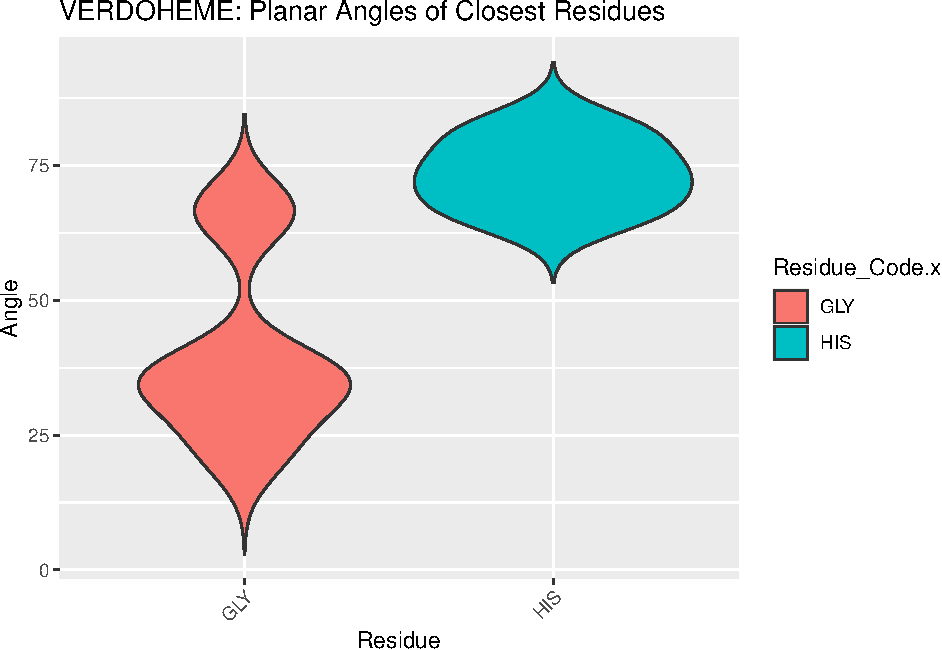
\includegraphics{_main_files/figure-latex/VERDOHEME-planarClosest-1.pdf}
\caption{\label{fig:VERDOHEME-planarClosest}VERDOHEME: Planar Angles of Closest Residues}
\end{figure}

\hypertarget{figs-cabAll}{%
\section{All CA-CB-Fe Angles}\label{figs-cabAll}}

\begin{figure}
\centering
\includegraphics{_main_files/figure-latex/HEM-cab-All-1.pdf}
\caption{\label{fig:HEM-cab-All}HEM: All CA-CB-Fe Angles}
\end{figure}

\begin{figure}
\centering
\includegraphics{_main_files/figure-latex/HEC-cab-All-1.pdf}
\caption{\label{fig:HEC-cab-All}HEC: All CA-CB-Fe Angles}
\end{figure}

\begin{figure}
\centering
\includegraphics{_main_files/figure-latex/SRM-cab-All-1.pdf}
\caption{\label{fig:SRM-cab-All}SRM: All CA-CB-Fe Angles}
\end{figure}

\begin{figure}
\centering
\includegraphics{_main_files/figure-latex/VERDOHEME-cab-All-1.pdf}
\caption{\label{fig:VERDOHEME-cab-All}VERDOHEME: All CA-CB-Fe Angles}
\end{figure}

\hypertarget{figs-cabClosest}{%
\section{CA-CB-Fe Angles of Closest Residues}\label{figs-cabClosest}}

\begin{figure}
\centering
\includegraphics{_main_files/figure-latex/HEM-cabClosest-1.pdf}
\caption{\label{fig:HEM-cabClosest}HEM: CACBFe Angles of Closest Residues}
\end{figure}

\begin{figure}
\centering
\includegraphics{_main_files/figure-latex/HEC-cabClosest-1.pdf}
\caption{\label{fig:HEC-cabClosest}HEC: CACBFe Angles of Closest Residues}
\end{figure}

\begin{figure}
\centering
\includegraphics{_main_files/figure-latex/SRM-cabClosest-1.pdf}
\caption{\label{fig:SRM-cabClosest}SRM: CACBFe Angles of Closest Residues}
\end{figure}

\begin{figure}
\centering
\includegraphics{_main_files/figure-latex/VERDOHEME-cabClosest-1.pdf}
\caption{\label{fig:VERDOHEME-cabClosest}VERDOHEME: CACBFe Angles of Closest Residues}
\end{figure}

\hypertarget{a-tables}{%
\chapter{Tables}\label{a-tables}}

\hypertarget{molOrgSec}{%
\section{Molecule Names and Source Organisms}\label{molOrgSec}}

\begin{longtabu} to \linewidth {>{\raggedright}X>{\raggedright}X>{\raggedright}X}
\caption{\label{tab:HEM-molOrg}HEM: Molecules and Source Organisms}\\
\toprule
\rotatebox{45}{PDB\_ID} & \rotatebox{45}{Molecule\_Name} & \rotatebox{45}{Source\_Organism}\\
\midrule
\endfirsthead
\caption[]{\label{tab:HEM-molOrg}HEM: Molecules and Source Organisms \textit{(continued)}}\\
\toprule
\rotatebox{45}{PDB\_ID} & \rotatebox{45}{Molecule\_Name} & \rotatebox{45}{Source\_Organism}\\
\midrule
\endhead

\endfoot
\bottomrule
\endlastfoot
\cellcolor{gray!6}{1B2V} & \cellcolor{gray!6}{PROTEIN (HEME-BINDING PROTEIN A);} & \cellcolor{gray!6}{SERRATIA MARCESCENS;}\\
1B5M & CYTOCHROME B5; & RATTUS NORVEGICUS;\\
\cellcolor{gray!6}{1DK0} & \cellcolor{gray!6}{HEME-BINDING PROTEIN A;} & \cellcolor{gray!6}{SERRATIA MARCESCENS;}\\
1DKH & HEME-BINDING PROTEIN A; & SERRATIA MARCESCENS;\\
\cellcolor{gray!6}{1ICC} & \cellcolor{gray!6}{CYTOCHROME B5 OUTER MITOCHONDRIAL MEMBRANE} & \cellcolor{gray!6}{RATTUS NORVEGICUS;}\\
\addlinespace
1IPH & CATALASE HPII; & ESCHERICHIA COLI;\\
\cellcolor{gray!6}{1N45} & \cellcolor{gray!6}{HEME OXYGENASE 1;} & \cellcolor{gray!6}{HOMO SAPIENS;}\\
1P3T & HEME OXYGENASE 1; & NEISSERIA MENINGITIDIS;\\
\cellcolor{gray!6}{1QHU} & \cellcolor{gray!6}{PROTEIN (HEMOPEXIN);} & \cellcolor{gray!6}{ORYCTOLAGUS CUNICULUS;}\\
1QJS & HEMOPEXIN; & ORYCTOLAGUS CUNICULUS;\\
\addlinespace
\cellcolor{gray!6}{1SI8} & \cellcolor{gray!6}{CATALASE;} & \cellcolor{gray!6}{ENTEROCOCCUS FAECALIS;}\\
1SY2 & NITROPHORIN 4; & RHODNIUS PROLIXUS;\\
\cellcolor{gray!6}{1U9U} & \cellcolor{gray!6}{CYTOCHROME B5;} & \cellcolor{gray!6}{BOS TAURUS;}\\
1VGI & HEME OXYGENASE 1; & RATTUS NORVEGICUS;\\
\cellcolor{gray!6}{1ZVI} & \cellcolor{gray!6}{NITRIC-OXIDE SYNTHASE, BRAIN;} & \cellcolor{gray!6}{RATTUS NORVEGICUS;}\\
\addlinespace
2BHJ & NITRIC OXIDE SYNTHASE; & MUS MUSCULUS;\\
\cellcolor{gray!6}{2CJ0} & \cellcolor{gray!6}{CHLOROPEROXIDASE;} & \cellcolor{gray!6}{CALDARIOMYCES FUMAGO;}\\
2CN4 & HEMOPHORE HASA; & SERRATIA MARCESCENS;\\
\cellcolor{gray!6}{2CPO} & \cellcolor{gray!6}{CHLOROPEROXIDASE;} & \cellcolor{gray!6}{LEPTOXYPHIUM FUMAGO;}\\
2E2Y & MYOGLOBIN; & PHYSETER CATODON;\\
\addlinespace
\cellcolor{gray!6}{2FC2} & \cellcolor{gray!6}{NITRIC OXIDE SYNTHASE;} & \cellcolor{gray!6}{BACILLUS SUBTILIS;}\\
2IIZ & MELANIN BIOSYNTHESIS PROTEIN TYRA, PUTATIVE; & SHEWANELLA ONEIDENSIS;\\
\cellcolor{gray!6}{2IPS} & \cellcolor{gray!6}{LACTOPEROXIDASE;} & \cellcolor{gray!6}{BOS TAURUS;}\\
2J0P & HEMIN TRANSPORT PROTEIN HEMS; & YERSINIA ENTEROCOLITICA;\\
\cellcolor{gray!6}{2J18} & \cellcolor{gray!6}{CHLOROPEROXIDASE;} & \cellcolor{gray!6}{CALDARIOMYCES FUMAGO;}\\
\addlinespace
2O6P & IRON-REGULATED SURFACE DETERMINANT PROTEIN C; & STAPHYLOCOCCUS AUREUS SUBSP. AUREUS;\\
\cellcolor{gray!6}{2Q6N} & \cellcolor{gray!6}{CYTOCHROME P450 2B4;} & \cellcolor{gray!6}{ORYCTOLAGUS CUNICULUS;}\\
2R7A & BACTERIAL HEME BINDING PROTEIN; & SHIGELLA DYSENTERIAE;\\
\cellcolor{gray!6}{2SPL} & \cellcolor{gray!6}{MYOGLOBIN;} & \cellcolor{gray!6}{PHYSETER CATODON;}\\
2VEB & PROTOGLOBIN; & METHANOSARCINA ACETIVORANS;\\
\addlinespace
\cellcolor{gray!6}{3HX9} & \cellcolor{gray!6}{PROTEIN RV3592;} & \cellcolor{gray!6}{MYCOBACTERIUM TUBERCULOSIS;}\\
3MVF & NITROPHORIN-4; & RHODNIUS PROLIXUS;\\
\cellcolor{gray!6}{3QZN} & \cellcolor{gray!6}{IRON-REGULATED SURFACE DETERMINANT PROTEIN A;} & \cellcolor{gray!6}{STAPHYLOCOCCUS AUREUS SUBSP. AUREUS;}\\
3QZZ & METHANOSARCINA ACETIVORANS PROTOGLOBIN; & METHANOSARCINA ACETIVORANS;\\
\cellcolor{gray!6}{3SIK} & \cellcolor{gray!6}{CONSERVED DOMAIN PROTEIN;} & \cellcolor{gray!6}{BACILLUS ANTHRACIS;}\\
\addlinespace
3TGC & NITROPHORIN-4; & RHODNIUS PROLIXUS;\\
\cellcolor{gray!6}{3VP5} & \cellcolor{gray!6}{TRANSCRIPTIONAL REGULATOR;} & \cellcolor{gray!6}{LACTOCOCCUS LACTIS;}\\
3ZJS & PROTOGLOBIN; & METHANOSARCINA ACETIVORANS;\\
\cellcolor{gray!6}{4B8N} & \cellcolor{gray!6}{CYTOCHROME B5-HOST ORIGIN;} & \cellcolor{gray!6}{OSTREOCOCCUS TAURI VIRUS 2;}\\
4CAT & CATALASE; & PENICILLIUM JANTHINELLUM;\\
\addlinespace
\cellcolor{gray!6}{4CDP} & \cellcolor{gray!6}{PUTATIVE HEME/HEMOGLOBIN TRANSPORT PROTEIN;} & \cellcolor{gray!6}{ESCHERICHIA COLI;}\\
4I3Q & CYTOCHROME P450 3A4; & HOMO SAPIENS;\\
\cellcolor{gray!6}{4JET} & \cellcolor{gray!6}{HEMOPHORE HASA;} & \cellcolor{gray!6}{YERSINIA PESTIS;}\\
4MF9 & HEMIN DEGRADING FACTOR; & PSEUDOMONAS AERUGINOSA;\\
\cellcolor{gray!6}{4MYP} & \cellcolor{gray!6}{IRON-REGULATED SURFACE DETERMINANT PROTEIN A;} & \cellcolor{gray!6}{LISTERIA MONOCYTOGENES;}\\
\addlinespace
4NL5 & HEME-DEGRADING MONOOXYGENASE HMOB; & MYCOBACTERIUM TUBERCULOSIS;\\
\cellcolor{gray!6}{4UZV} & \cellcolor{gray!6}{HEMOGLOBIN;} & \cellcolor{gray!6}{THERMOBIFIDA FUSCA TM51;}\\
4XZD & EXTRACELLULAR HEME ACQUISITION HEMOPHORE HASA; & YERSINIA PSEUDOTUBERCULOSIS IP 32953;\\
\cellcolor{gray!6}{4Y1Q} & \cellcolor{gray!6}{EXTRACELLULAR HEME ACQUISITION HEMOPHORE HASA;} & \cellcolor{gray!6}{YERSINIA PSEUDOTUBERCULOSIS IP 32953;}\\
5CN5 & MYOGLOBIN; & EQUUS CABALLUS;\\
\addlinespace
\cellcolor{gray!6}{5GJ3} & \cellcolor{gray!6}{PERIPLASMIC BINDING PROTEIN;} & \cellcolor{gray!6}{ROSEIFLEXUS SP. RS-1;}\\
5KZL & HEME OXYGENASE; & LEPTOSPIRA INTERROGANS;\\
\cellcolor{gray!6}{5O1L} & \cellcolor{gray!6}{RUBBER OXYGENASE;} & \cellcolor{gray!6}{STREPTOMYCES SP. (STRAIN K30);}\\
5O1M & RUBBER OXYGENASE; & STREPTOMYCES SP. (STRAIN K30);\\
\cellcolor{gray!6}{5VEU} & \cellcolor{gray!6}{CYTOCHROME P450 3A5;} & \cellcolor{gray!6}{HOMO SAPIENS;}\\
\addlinespace
6A2J & HEME A SYNTHASE; & BACILLUS SUBTILIS (STRAIN 168);\\
\cellcolor{gray!6}{7C74} & \cellcolor{gray!6}{LACTOPEROXIDASE;} & \cellcolor{gray!6}{BOS MUTUS;}\\
7DMR & LACTOPEROXIDASE; & BOS MUTUS;\\*
\end{longtabu}

\begin{longtabu} to \linewidth {>{\raggedright}X>{\raggedright}X>{\raggedright}X}
\caption{\label{tab:HEC-molOrg}HEC: Molecules and Source Organisms}\\
\toprule
\rotatebox{45}{PDB\_ID} & \rotatebox{45}{Molecule\_Name} & \rotatebox{45}{Source\_Organism}\\
\midrule
\endfirsthead
\caption[]{\label{tab:HEC-molOrg}HEC: Molecules and Source Organisms \textit{(continued)}}\\
\toprule
\rotatebox{45}{PDB\_ID} & \rotatebox{45}{Molecule\_Name} & \rotatebox{45}{Source\_Organism}\\
\midrule
\endhead

\endfoot
\bottomrule
\endlastfoot
\cellcolor{gray!6}{1BBH} & \cellcolor{gray!6}{CYTOCHROME C';} & \cellcolor{gray!6}{ALLOCHROMATIUM VINOSUM;}\\
1S56 & HEMOGLOBIN-LIKE PROTEIN HBN; & MYCOBACTERIUM TUBERCULOSIS;\\
\cellcolor{gray!6}{1W2L} & \cellcolor{gray!6}{CYTOCHROME OXIDASE SUBUNIT II;} & \cellcolor{gray!6}{RHODOTHERMUS MARINUS;}\\
2BC5 & SOLUBLE CYTOCHROME B562; & ESCHERICHIA COLI;\\
\cellcolor{gray!6}{2BH5} & \cellcolor{gray!6}{CYTOCHROME C-550;} & \cellcolor{gray!6}{PARACOCCUS VERSUTUS;}\\
\addlinespace
3EAH & NITRIC OXIDE SYNTHASE, ENDOTHELIAL; & HOMO SAPIENS;\\
\cellcolor{gray!6}{3X15} & \cellcolor{gray!6}{CYTOCHROME C552;} & \cellcolor{gray!6}{AQUIFEX AEOLICUS VF5;}\\
5KPF & CYTOCHROME C ISO-1; & SACCHAROMYCES CEREVISIAE;\\
\cellcolor{gray!6}{5LFT} & \cellcolor{gray!6}{CYTOCHROME C ISO-1;} & \cellcolor{gray!6}{SACCHAROMYCES CEREVISIAE;}\\
5T8W & CYC1P; & SACCHAROMYCES CEREVISIAE;\\
\addlinespace
\cellcolor{gray!6}{6VDQ} & \cellcolor{gray!6}{3-METHYL-L-TYROSINE PEROXYGENASE;} & \cellcolor{gray!6}{STREPTOMYCES LAVENDULAE;}\\
6WZA & SOLUBLE CYTOCHROME B562; & ESCHERICHIA COLI;\\
\cellcolor{gray!6}{6XNK} & \cellcolor{gray!6}{CYTOCHROME C;} & \cellcolor{gray!6}{HOMO SAPIENS;}\\*
\end{longtabu}

\begin{longtabu} to \linewidth {>{\raggedright}X>{\raggedright}X>{\raggedright}X}
\caption{\label{tab:SRM-molOrg}SRM: Molecules and Source Organisms}\\
\toprule
\rotatebox{45}{PDB\_ID} & \rotatebox{45}{Molecule\_Name} & \rotatebox{45}{Source\_Organism}\\
\midrule
\endfirsthead
\caption[]{\label{tab:SRM-molOrg}SRM: Molecules and Source Organisms \textit{(continued)}}\\
\toprule
\rotatebox{45}{PDB\_ID} & \rotatebox{45}{Molecule\_Name} & \rotatebox{45}{Source\_Organism}\\
\midrule
\endhead

\endfoot
\bottomrule
\endlastfoot
\cellcolor{gray!6}{1ZJ8} & \cellcolor{gray!6}{PROBABLE FERREDOXIN-DEPENDENT NITRITE REDUCTASE NIRA;} & \cellcolor{gray!6}{MYCOBACTERIUM TUBERCULOSIS;}\\
2AKJ & FERREDOXIN--NITRITE REDUCTASE, CHLOROPLAST; & SPINACIA OLERACEA;\\
\cellcolor{gray!6}{2AOP} & \cellcolor{gray!6}{SULFITE REDUCTASE HEMOPROTEIN;} & \cellcolor{gray!6}{ESCHERICHIA COLI;}\\
3B0G & NITRITE REDUCTASE; & NICOTIANA TABACUM;\\
\cellcolor{gray!6}{3VKP} & \cellcolor{gray!6}{NITRITE REDUCTASE;} & \cellcolor{gray!6}{NICOTIANA TABACUM;}\\
\addlinespace
3VLX & NITRITE REDUCTASE; & NICOTIANA TABACUM;\\
\cellcolor{gray!6}{3VLY} & \cellcolor{gray!6}{NITRITE REDUCTASE;} & \cellcolor{gray!6}{NICOTIANA TABACUM;}\\
3VLZ & NITRITE REDUCTASE; & NICOTIANA TABACUM;\\
\cellcolor{gray!6}{5H8V} & \cellcolor{gray!6}{SULFITE REDUCTASE [FERREDOXIN], CHLOROPLASTIC;} & \cellcolor{gray!6}{ZEA MAYS;}\\*
\end{longtabu}

\begin{longtabu} to \linewidth {>{\raggedright}X>{\raggedright}X>{\raggedright}X}
\caption{\label{tab:VERDOHEME-molOrg}VERDOHEME: Molecules and Source Organisms}\\
\toprule
\rotatebox{45}{PDB\_ID} & \rotatebox{45}{Molecule\_Name} & \rotatebox{45}{Source\_Organism}\\
\midrule
\endfirsthead
\caption[]{\label{tab:VERDOHEME-molOrg}VERDOHEME: Molecules and Source Organisms \textit{(continued)}}\\
\toprule
\rotatebox{45}{PDB\_ID} & \rotatebox{45}{Molecule\_Name} & \rotatebox{45}{Source\_Organism}\\
\midrule
\endhead

\endfoot
\bottomrule
\endlastfoot
\cellcolor{gray!6}{2ZVU} & \cellcolor{gray!6}{HEME OXYGENASE 1;} & \cellcolor{gray!6}{RATTUS NORVEGICUS;}\\
3MOO & HEME OXYGENASE; & CORYNEBACTERIUM DIPHTHERIAE;\\
\cellcolor{gray!6}{1TWN} & \cellcolor{gray!6}{HEME OXYGENASE 1;} & \cellcolor{gray!6}{HOMO SAPIENS;}\\
1TWR & HEME OXYGENASE 1; & HOMO SAPIENS;\\*
\end{longtabu}

\hypertarget{volume-and-surface-areas}{%
\section{Volume and Surface Areas}\label{volume-and-surface-areas}}

\begin{longtabu} to \linewidth {>{\raggedright}X>{\raggedleft}X>{\raggedleft}X>{\raggedleft}X>{\raggedleft}X>{\raggedleft}X}
\caption{\label{tab:HEM-volSA}HEM: Volume and Surface Areas}\\
\toprule
\rotatebox{45}{PDB\_ID} & \rotatebox{45}{Volume\_Data} & \rotatebox{45}{HEM\_Excluded\_SA} & \rotatebox{45}{HEM\_Accessible\_SA} & \rotatebox{45}{Pocket\_Excluded\_SA} & \rotatebox{45}{Pocket\_Accessible\_SA}\\
\midrule
\endfirsthead
\caption[]{\label{tab:HEM-volSA}HEM: Volume and Surface Areas \textit{(continued)}}\\
\toprule
\rotatebox{45}{PDB\_ID} & \rotatebox{45}{Volume\_Data} & \rotatebox{45}{HEM\_Excluded\_SA} & \rotatebox{45}{HEM\_Accessible\_SA} & \rotatebox{45}{Pocket\_Excluded\_SA} & \rotatebox{45}{Pocket\_Accessible\_SA}\\
\midrule
\endhead

\endfoot
\bottomrule
\endlastfoot
\cellcolor{gray!6}{1B2V} & \cellcolor{gray!6}{893.60} & \cellcolor{gray!6}{502.042} & \cellcolor{gray!6}{820.988} & \cellcolor{gray!6}{7276.09} & \cellcolor{gray!6}{8232.60}\\
1B5M & 672.79 & 490.050 & 800.780 & 4695.01 & 5512.20\\
\cellcolor{gray!6}{1DK0} & \cellcolor{gray!6}{966.72} & \cellcolor{gray!6}{505.258} & \cellcolor{gray!6}{837.157} & \cellcolor{gray!6}{7237.94} & \cellcolor{gray!6}{8217.58}\\
1DKH & 1010.70 & 509.042 & 828.131 & 7402.34 & 8175.94\\
\cellcolor{gray!6}{1ICC} & \cellcolor{gray!6}{1000.40} & \cellcolor{gray!6}{499.585} & \cellcolor{gray!6}{811.357} & \cellcolor{gray!6}{5079.72} & \cellcolor{gray!6}{6028.23}\\
\addlinespace
1IPH & 1345.60 & 501.603 & 814.652 & 33983.80 & 34094.40\\
\cellcolor{gray!6}{1N45} & \cellcolor{gray!6}{978.98} & \cellcolor{gray!6}{560.384} & \cellcolor{gray!6}{983.238} & \cellcolor{gray!6}{9944.50} & \cellcolor{gray!6}{10779.30}\\
1P3T & 987.05 & 509.939 & 829.611 & 9530.67 & 10410.80\\
\cellcolor{gray!6}{1QHU} & \cellcolor{gray!6}{1389.20} & \cellcolor{gray!6}{573.686} & \cellcolor{gray!6}{1002.160} & \cellcolor{gray!6}{18503.10} & \cellcolor{gray!6}{18257.20}\\
1QJS & 1102.30 & 573.266 & 1000.380 & 18588.40 & 18584.10\\
\addlinespace
\cellcolor{gray!6}{1SI8} & \cellcolor{gray!6}{965.57} & \cellcolor{gray!6}{646.643} & \cellcolor{gray!6}{1184.070} & \cellcolor{gray!6}{23711.20} & \cellcolor{gray!6}{25120.40}\\
1SY2 & 918.34 & 501.850 & 817.749 & 8960.76 & 9610.23\\
\cellcolor{gray!6}{1U9U} & \cellcolor{gray!6}{738.55} & \cellcolor{gray!6}{496.132} & \cellcolor{gray!6}{813.773} & \cellcolor{gray!6}{4675.76} & \cellcolor{gray!6}{5632.32}\\
1VGI & 870.44 & 577.234 & 1002.530 & 9615.29 & 10248.20\\
\cellcolor{gray!6}{1ZVI} & \cellcolor{gray!6}{1435.90} & \cellcolor{gray!6}{701.091} & \cellcolor{gray!6}{1129.540} & \cellcolor{gray!6}{19918.60} & \cellcolor{gray!6}{20968.20}\\
\addlinespace
2BHJ & 1438.30 & 836.576 & 1290.530 & 20102.30 & 20762.60\\
\cellcolor{gray!6}{2CJ0} & \cellcolor{gray!6}{809.62} & \cellcolor{gray!6}{2653.180} & \cellcolor{gray!6}{4835.280} & \cellcolor{gray!6}{12749.60} & \cellcolor{gray!6}{12892.20}\\
2CN4 & 526.88 & 576.760 & 961.348 & 9617.23 & 11917.70\\
\cellcolor{gray!6}{2CPO} & \cellcolor{gray!6}{886.17} & \cellcolor{gray!6}{1846.490} & \cellcolor{gray!6}{3329.540} & \cellcolor{gray!6}{13081.60} & \cellcolor{gray!6}{12995.60}\\
2E2Y & 994.92 & 811.270 & 1607.370 & 7531.94 & 8240.75\\
\addlinespace
\cellcolor{gray!6}{2FC2} & \cellcolor{gray!6}{1091.40} & \cellcolor{gray!6}{1011.190} & \cellcolor{gray!6}{1669.900} & \cellcolor{gray!6}{18383.50} & \cellcolor{gray!6}{18552.10}\\
2IIZ & 1015.60 & 731.342 & 1393.160 & 13651.70 & 14031.40\\
\cellcolor{gray!6}{2IPS} & \cellcolor{gray!6}{1242.40} & \cellcolor{gray!6}{618.252} & \cellcolor{gray!6}{1075.560} & \cellcolor{gray!6}{27760.50} & \cellcolor{gray!6}{25814.10}\\
2J0P & 1281.80 & 1030.510 & 1873.810 & 15192.90 & 15871.10\\
\cellcolor{gray!6}{2J18} & \cellcolor{gray!6}{841.67} & \cellcolor{gray!6}{1962.990} & \cellcolor{gray!6}{3556.340} & \cellcolor{gray!6}{12675.10} & \cellcolor{gray!6}{12779.00}\\
\addlinespace
2O6P & 788.05 & 499.017 & 822.121 & 6234.84 & 7200.43\\
\cellcolor{gray!6}{2Q6N} & \cellcolor{gray!6}{1030.10} & \cellcolor{gray!6}{644.365} & \cellcolor{gray!6}{1040.080} & \cellcolor{gray!6}{20051.10} & \cellcolor{gray!6}{19747.50}\\
2R7A & 1284.50 & 507.098 & 845.182 & 11255.10 & 12389.00\\
\cellcolor{gray!6}{2SPL} & \cellcolor{gray!6}{1055.70} & \cellcolor{gray!6}{589.706} & \cellcolor{gray!6}{1029.660} & \cellcolor{gray!6}{7588.36} & \cellcolor{gray!6}{8105.94}\\
2VEB & 886.06 & 762.309 & 1454.750 & 9840.72 & 10401.80\\
\addlinespace
\cellcolor{gray!6}{3HX9} & \cellcolor{gray!6}{1844.50} & \cellcolor{gray!6}{785.442} & \cellcolor{gray!6}{1168.200} & \cellcolor{gray!6}{5819.08} & \cellcolor{gray!6}{7189.03}\\
3MVF & 1271.40 & 576.502 & 1009.950 & 8559.24 & 9573.08\\
\cellcolor{gray!6}{3QZN} & \cellcolor{gray!6}{726.52} & \cellcolor{gray!6}{664.858} & \cellcolor{gray!6}{1221.330} & \cellcolor{gray!6}{6133.24} & \cellcolor{gray!6}{7179.49}\\
3QZZ & 977.30 & 496.950 & 825.255 & 8523.59 & 9708.28\\
\cellcolor{gray!6}{3SIK} & \cellcolor{gray!6}{492.15} & \cellcolor{gray!6}{498.621} & \cellcolor{gray!6}{823.565} & \cellcolor{gray!6}{6495.38} & \cellcolor{gray!6}{7739.06}\\
\addlinespace
3TGC & 969.87 & 524.380 & 853.710 & 8712.77 & 9181.94\\
\cellcolor{gray!6}{3VP5} & \cellcolor{gray!6}{1094.60} & \cellcolor{gray!6}{602.790} & \cellcolor{gray!6}{1050.820} & \cellcolor{gray!6}{9801.82} & \cellcolor{gray!6}{10810.80}\\
3ZJS & 788.74 & 528.419 & 860.137 & 9568.10 & 10130.40\\
\cellcolor{gray!6}{4B8N} & \cellcolor{gray!6}{841.27} & \cellcolor{gray!6}{569.302} & \cellcolor{gray!6}{990.216} & \cellcolor{gray!6}{4560.39} & \cellcolor{gray!6}{5458.66}\\
4CAT & 1933.90 & 484.341 & 778.502 & 28372.40 & 36788.30\\
\addlinespace
\cellcolor{gray!6}{4CDP} & \cellcolor{gray!6}{1053.70} & \cellcolor{gray!6}{1425.050} & \cellcolor{gray!6}{3141.090} & \cellcolor{gray!6}{14733.50} & \cellcolor{gray!6}{15887.40}\\
4I3Q & 1220.50 & 510.623 & 845.108 & 21946.50 & 21093.70\\
\cellcolor{gray!6}{4JET} & \cellcolor{gray!6}{1010.80} & \cellcolor{gray!6}{495.992} & \cellcolor{gray!6}{818.131} & \cellcolor{gray!6}{7887.81} & \cellcolor{gray!6}{8695.85}\\
4MF9 & 1286.50 & 488.695 & 790.732 & 15669.80 & 16791.30\\
\cellcolor{gray!6}{4MYP} & \cellcolor{gray!6}{610.72} & \cellcolor{gray!6}{963.019} & \cellcolor{gray!6}{1834.680} & \cellcolor{gray!6}{6285.40} & \cellcolor{gray!6}{7351.53}\\
\addlinespace
4NL5 & 1088.70 & 576.669 & 1003.400 & 5715.52 & 6894.72\\
\cellcolor{gray!6}{4UZV} & \cellcolor{gray!6}{1184.10} & \cellcolor{gray!6}{526.584} & \cellcolor{gray!6}{844.058} & \cellcolor{gray!6}{7378.28} & \cellcolor{gray!6}{8322.74}\\
4XZD & 932.14 & 498.788 & 816.032 & 8028.32 & 8752.50\\
\cellcolor{gray!6}{4Y1Q} & \cellcolor{gray!6}{952.23} & \cellcolor{gray!6}{494.939} & \cellcolor{gray!6}{806.960} & \cellcolor{gray!6}{7905.84} & \cellcolor{gray!6}{8785.04}\\
5CN5 & 1070.30 & 663.162 & 1223.640 & 7629.45 & 8117.34\\
\addlinespace
\cellcolor{gray!6}{5GJ3} & \cellcolor{gray!6}{1108.20} & \cellcolor{gray!6}{756.603} & \cellcolor{gray!6}{1131.670} & \cellcolor{gray!6}{11394.00} & \cellcolor{gray!6}{12591.80}\\
5KZL & 914.22 & 483.760 & 805.567 & 9662.03 & 10431.00\\
\cellcolor{gray!6}{5O1L} & \cellcolor{gray!6}{1438.70} & \cellcolor{gray!6}{801.519} & \cellcolor{gray!6}{1447.270} & \cellcolor{gray!6}{15538.20} & \cellcolor{gray!6}{16876.00}\\
5O1M & 1431.30 & 493.850 & 799.331 & 16096.90 & 15912.50\\
\cellcolor{gray!6}{5VEU} & \cellcolor{gray!6}{964.76} & \cellcolor{gray!6}{993.578} & \cellcolor{gray!6}{1502.660} & \cellcolor{gray!6}{20900.80} & \cellcolor{gray!6}{20425.90}\\
\addlinespace
6A2J & 1015.90 & 6183.450 & 9902.920 & 14870.30 & 15888.00\\
\cellcolor{gray!6}{7C74} & \cellcolor{gray!6}{1155.10} & \cellcolor{gray!6}{497.527} & \cellcolor{gray!6}{820.381} & \cellcolor{gray!6}{26111.40} & \cellcolor{gray!6}{25094.20}\\
7DMR & 1083.40 & 1049.750 & 1916.950 & 26004.00 & 24563.80\\*
\end{longtabu}

\begin{longtabu} to \linewidth {>{\raggedright}X>{\raggedleft}X>{\raggedleft}X>{\raggedleft}X>{\raggedleft}X>{\raggedleft}X}
\caption{\label{tab:HEC-volSA}HEC: Volume and Surface Areas}\\
\toprule
\rotatebox{45}{PDB\_ID} & \rotatebox{45}{Volume\_Data} & \rotatebox{45}{HEC\_Excluded\_SA} & \rotatebox{45}{HEC\_Accessible\_SA} & \rotatebox{45}{Pocket\_Excluded\_SA} & \rotatebox{45}{Pocket\_Accessible\_SA}\\
\midrule
\endfirsthead
\caption[]{\label{tab:HEC-volSA}HEC: Volume and Surface Areas \textit{(continued)}}\\
\toprule
\rotatebox{45}{PDB\_ID} & \rotatebox{45}{Volume\_Data} & \rotatebox{45}{HEC\_Excluded\_SA} & \rotatebox{45}{HEC\_Accessible\_SA} & \rotatebox{45}{Pocket\_Excluded\_SA} & \rotatebox{45}{Pocket\_Accessible\_SA}\\
\midrule
\endhead

\endfoot
\bottomrule
\endlastfoot
\cellcolor{gray!6}{1BBH} & \cellcolor{gray!6}{969.51} & \cellcolor{gray!6}{514.130} & \cellcolor{gray!6}{829.817} & \cellcolor{gray!6}{6441.44} & \cellcolor{gray!6}{7514.06}\\
1S56 & 1103.60 & 643.733 & 1075.840 & 6711.26 & 7477.96\\
\cellcolor{gray!6}{1W2L} & \cellcolor{gray!6}{756.08} & \cellcolor{gray!6}{702.711} & \cellcolor{gray!6}{1240.680} & \cellcolor{gray!6}{5042.58} & \cellcolor{gray!6}{5485.50}\\
2BC5 & 1166.20 & 569.905 & 997.324 & 5489.91 & 6306.02\\
\cellcolor{gray!6}{2BH5} & \cellcolor{gray!6}{814.15} & \cellcolor{gray!6}{508.637} & \cellcolor{gray!6}{844.494} & \cellcolor{gray!6}{6359.51} & \cellcolor{gray!6}{6975.70}\\
\addlinespace
3EAH & 1280.90 & 993.430 & 1697.130 & 18413.40 & 19313.80\\
\cellcolor{gray!6}{3X15} & \cellcolor{gray!6}{823.59} & \cellcolor{gray!6}{496.328} & \cellcolor{gray!6}{802.584} & \cellcolor{gray!6}{5722.90} & \cellcolor{gray!6}{7493.62}\\
5KPF & 778.79 & 568.036 & 1007.680 & 5485.51 & 6155.84\\
\cellcolor{gray!6}{5LFT} & \cellcolor{gray!6}{809.40} & \cellcolor{gray!6}{1720.870} & \cellcolor{gray!6}{2719.000} & \cellcolor{gray!6}{5539.47} & \cellcolor{gray!6}{6315.96}\\
5T8W & 858.74 & 511.519 & 848.952 & 5755.48 & 6458.40\\
\addlinespace
\cellcolor{gray!6}{6VDQ} & \cellcolor{gray!6}{977.52} & \cellcolor{gray!6}{510.534} & \cellcolor{gray!6}{846.299} & \cellcolor{gray!6}{13399.60} & \cellcolor{gray!6}{14076.40}\\
6WZA & 1040.10 & 713.997 & 1095.240 & 5529.40 & 6385.75\\
\cellcolor{gray!6}{6XNK} & \cellcolor{gray!6}{2214.40} & \cellcolor{gray!6}{499.687} & \cellcolor{gray!6}{835.610} & \cellcolor{gray!6}{6737.92} & \cellcolor{gray!6}{8143.17}\\*
\end{longtabu}

\begin{longtabu} to \linewidth {>{\raggedright}X>{\raggedleft}X>{\raggedleft}X>{\raggedleft}X>{\raggedleft}X>{\raggedleft}X}
\caption{\label{tab:SRM-volSA}SRM: Volume and Surface Areas}\\
\toprule
\rotatebox{45}{PDB\_ID} & \rotatebox{45}{Volume\_Data} & \rotatebox{45}{SRM\_Excluded\_SA} & \rotatebox{45}{SRM\_Accessible\_SA} & \rotatebox{45}{Pocket\_Excluded\_SA} & \rotatebox{45}{Pocket\_Accessible\_SA}\\
\midrule
\endfirsthead
\caption[]{\label{tab:SRM-volSA}SRM: Volume and Surface Areas \textit{(continued)}}\\
\toprule
\rotatebox{45}{PDB\_ID} & \rotatebox{45}{Volume\_Data} & \rotatebox{45}{SRM\_Excluded\_SA} & \rotatebox{45}{SRM\_Accessible\_SA} & \rotatebox{45}{Pocket\_Excluded\_SA} & \rotatebox{45}{Pocket\_Accessible\_SA}\\
\midrule
\endhead

\endfoot
\bottomrule
\endlastfoot
\cellcolor{gray!6}{1ZJ8} & \cellcolor{gray!6}{1960.2} & \cellcolor{gray!6}{656.508} & \cellcolor{gray!6}{1036.43} & \cellcolor{gray!6}{20388.7} & \cellcolor{gray!6}{21432.8}\\
2AKJ & 1810.2 & 659.667 & 1041.00 & 21673.6 & 20933.7\\
\cellcolor{gray!6}{2AOP} & \cellcolor{gray!6}{1040.5} & \cellcolor{gray!6}{682.170} & \cellcolor{gray!6}{1045.18} & \cellcolor{gray!6}{18119.8} & \cellcolor{gray!6}{18016.0}\\
3B0G & 1189.9 & 666.995 & 1054.40 & 21496.8 & 21033.9\\
\cellcolor{gray!6}{3VKP} & \cellcolor{gray!6}{1178.0} & \cellcolor{gray!6}{675.050} & \cellcolor{gray!6}{1049.85} & \cellcolor{gray!6}{21279.3} & \cellcolor{gray!6}{20964.9}\\
\addlinespace
3VLX & 1164.8 & 667.013 & 1052.76 & 21470.0 & 21037.0\\
\cellcolor{gray!6}{3VLY} & \cellcolor{gray!6}{1061.8} & \cellcolor{gray!6}{675.293} & \cellcolor{gray!6}{1046.41} & \cellcolor{gray!6}{21476.6} & \cellcolor{gray!6}{21022.1}\\
3VLZ & 1123.2 & 676.360 & 1051.40 & 21433.5 & 20901.8\\
\cellcolor{gray!6}{5H8V} & \cellcolor{gray!6}{1360.8} & \cellcolor{gray!6}{685.850} & \cellcolor{gray!6}{1052.56} & \cellcolor{gray!6}{22885.9} & \cellcolor{gray!6}{22713.3}\\*
\end{longtabu}

\begin{longtabu} to \linewidth {>{\raggedright}X>{\raggedright}X>{\raggedright}X>{\raggedright}X>{\raggedright}X>{\raggedright}X}
\caption{\label{tab:VERDOHEME-volSA}VERDOHEME: Volume and Surface Areas}\\
\toprule
\rotatebox{45}{PDB\_ID} & \rotatebox{45}{Volume\_Data} & \rotatebox{45}{VERDOHEME\_EXCLUDED\_SA} & \rotatebox{45}{VERDOHEME\_ACCESSIBLE\_SA} & \rotatebox{45}{POCKET\_EXCLUDED\_SA} & \rotatebox{45}{POCKET\_ACCESSIBLE\_SA}\\
\midrule
\endfirsthead
\caption[]{\label{tab:VERDOHEME-volSA}VERDOHEME: Volume and Surface Areas \textit{(continued)}}\\
\toprule
\rotatebox{45}{PDB\_ID} & \rotatebox{45}{Volume\_Data} & \rotatebox{45}{VERDOHEME\_EXCLUDED\_SA} & \rotatebox{45}{VERDOHEME\_ACCESSIBLE\_SA} & \rotatebox{45}{POCKET\_EXCLUDED\_SA} & \rotatebox{45}{POCKET\_ACCESSIBLE\_SA}\\
\midrule
\endhead

\endfoot
\bottomrule
\endlastfoot
\cellcolor{gray!6}{2ZVU} & \cellcolor{gray!6}{984.51} & \cellcolor{gray!6}{560.791} & \cellcolor{gray!6}{969.143} & \cellcolor{gray!6}{9633.81} & \cellcolor{gray!6}{10317.3}\\
3MOO & 864.48 & 870.228 & 1772.07 & 9371.88 & 10170.3\\
\cellcolor{gray!6}{1TWN} & \cellcolor{gray!6}{1145} & \cellcolor{gray!6}{448.81} & \cellcolor{gray!6}{759.632} & \cellcolor{gray!6}{9966.97} & \cellcolor{gray!6}{10896.8}\\
1TWR & 1426 & 469.982 & 783.313 & 9854.01 & 10775.6\\*
\end{longtabu}

\hypertarget{all-planar-angles}{%
\section{All Planar Angles}\label{all-planar-angles}}

\begin{longtabu} to \linewidth {>{\raggedright}X>{\raggedleft}X>{\raggedright}X>{\raggedleft}X>{\raggedright}X>{\raggedright}X}
\caption{\label{tab:HEM-t-planarAll}HEM: All Planar Angles}\\
\toprule
\rotatebox{45}{PDB\_ID} & \rotatebox{45}{Residue\_Number} & \rotatebox{45}{Residue\_Code.x} & \rotatebox{45}{Mean\_Distance} & \rotatebox{45}{Angle} & \rotatebox{45}{Residue\_Code.y}\\
\midrule
\endfirsthead
\caption[]{\label{tab:HEM-t-planarAll}HEM: All Planar Angles \textit{(continued)}}\\
\toprule
\rotatebox{45}{PDB\_ID} & \rotatebox{45}{Residue\_Number} & \rotatebox{45}{Residue\_Code.x} & \rotatebox{45}{Mean\_Distance} & \rotatebox{45}{Angle} & \rotatebox{45}{Residue\_Code.y}\\
\midrule
\endhead

\endfoot
\bottomrule
\endlastfoot
\cellcolor{gray!6}{1N45} & \cellcolor{gray!6}{28} & \cellcolor{gray!6}{ALA} & \cellcolor{gray!6}{6.981230} & \cellcolor{gray!6}{51.517} & \cellcolor{gray!6}{ALA}\\
2CJ0 & 31 & ALA & 5.440871 & 54.576 & ALA\\
\cellcolor{gray!6}{2CPO} & \cellcolor{gray!6}{31} & \cellcolor{gray!6}{ALA} & \cellcolor{gray!6}{5.505123} & \cellcolor{gray!6}{50.842} & \cellcolor{gray!6}{ALA}\\
2J18 & 31 & ALA & 5.457126 & 52.882 & ALA\\
\cellcolor{gray!6}{1SY2} & \cellcolor{gray!6}{42} & \cellcolor{gray!6}{ALA} & \cellcolor{gray!6}{6.006055} & \cellcolor{gray!6}{38.441} & \cellcolor{gray!6}{ALA}\\
\addlinespace
3MVF & 42 & ALA & 5.827660 & 37.714 & ALA\\
\cellcolor{gray!6}{3TGC} & \cellcolor{gray!6}{42} & \cellcolor{gray!6}{ALA} & \cellcolor{gray!6}{6.033598} & \cellcolor{gray!6}{36.906} & \cellcolor{gray!6}{ALA}\\
2O6P & 49 & ALA & 6.356063 & 33.301 & ALA\\
\cellcolor{gray!6}{4B8N} & \cellcolor{gray!6}{54} & \cellcolor{gray!6}{ALA} & \cellcolor{gray!6}{6.390793} & \cellcolor{gray!6}{40.757} & \cellcolor{gray!6}{ALA}\\
1B5M & 67 & ALA & 5.797296 & 4.944 & ALA\\
\addlinespace
\cellcolor{gray!6}{1ICC} & \cellcolor{gray!6}{67} & \cellcolor{gray!6}{ALA} & \cellcolor{gray!6}{6.085233} & \cellcolor{gray!6}{8.515} & \cellcolor{gray!6}{ALA}\\
1U9U & 67 & ALA & 6.016697 & 3.989 & ALA\\
\cellcolor{gray!6}{2CJ0} & \cellcolor{gray!6}{71} & \cellcolor{gray!6}{ALA} & \cellcolor{gray!6}{6.531120} & \cellcolor{gray!6}{88.775} & \cellcolor{gray!6}{ALA}\\
2CPO & 71 & ALA & 6.539227 & 89.067 & ALA\\
\cellcolor{gray!6}{2J18} & \cellcolor{gray!6}{71} & \cellcolor{gray!6}{ALA} & \cellcolor{gray!6}{6.477348} & \cellcolor{gray!6}{89.793} & \cellcolor{gray!6}{ALA}\\
\addlinespace
3HX9 & 71 & ALA & 6.230664 & 24.118 & ALA\\
\cellcolor{gray!6}{4NL5} & \cellcolor{gray!6}{71} & \cellcolor{gray!6}{ALA} & \cellcolor{gray!6}{6.805378} & \cellcolor{gray!6}{12.006} & \cellcolor{gray!6}{ALA}\\
4Y1Q & 75 & ALA & 6.722226 & 65.239 & ALA\\
\cellcolor{gray!6}{1P3T} & \cellcolor{gray!6}{121} & \cellcolor{gray!6}{ALA} & \cellcolor{gray!6}{6.382367} & \cellcolor{gray!6}{68.509} & \cellcolor{gray!6}{ALA}\\
3SIK & 138 & ALA & 6.231014 & 84.490 & ALA\\
\addlinespace
\cellcolor{gray!6}{3QZN} & \cellcolor{gray!6}{166} & \cellcolor{gray!6}{ALA} & \cellcolor{gray!6}{6.907969} & \cellcolor{gray!6}{73.637} & \cellcolor{gray!6}{ALA}\\
2R7A & 169 & ALA & 5.223004 & 39.141 & ALA\\
\cellcolor{gray!6}{6A2J} & \cellcolor{gray!6}{180} & \cellcolor{gray!6}{ALA} & \cellcolor{gray!6}{6.687029} & \cellcolor{gray!6}{46.961} & \cellcolor{gray!6}{ALA}\\
2BHJ & 191 & ALA & 6.261711 & 68.057 & ALA\\
\cellcolor{gray!6}{6A2J} & \cellcolor{gray!6}{220} & \cellcolor{gray!6}{ALA} & \cellcolor{gray!6}{5.986896} & \cellcolor{gray!6}{31.915} & \cellcolor{gray!6}{ALA}\\
\addlinespace
6A2J & 259 & ALA & 6.937825 & 66.152 & ALA\\
\cellcolor{gray!6}{4MYP} & \cellcolor{gray!6}{282} & \cellcolor{gray!6}{ALA} & \cellcolor{gray!6}{6.581195} & \cellcolor{gray!6}{36.442} & \cellcolor{gray!6}{ALA}\\
4MYP & 293 & ALA & 6.207799 & 64.118 & ALA\\
\cellcolor{gray!6}{2Q6N} & \cellcolor{gray!6}{298} & \cellcolor{gray!6}{ALA} & \cellcolor{gray!6}{5.672036} & \cellcolor{gray!6}{28.414} & \cellcolor{gray!6}{ALA}\\
4I3Q & 305 & ALA & 5.305272 & 55.811 & ALA\\
\addlinespace
\cellcolor{gray!6}{5VEU} & \cellcolor{gray!6}{305} & \cellcolor{gray!6}{ALA} & \cellcolor{gray!6}{6.219660} & \cellcolor{gray!6}{37.021} & \cellcolor{gray!6}{ALA}\\
1ZVI & 412 & ALA & 6.481380 & 68.137 & ALA\\
\cellcolor{gray!6}{2Q6N} & \cellcolor{gray!6}{442} & \cellcolor{gray!6}{ALA} & \cellcolor{gray!6}{6.935846} & \cellcolor{gray!6}{35.011} & \cellcolor{gray!6}{ALA}\\
5VEU & 447 & ALA & 6.667315 & 35.226 & ALA\\
\cellcolor{gray!6}{4I3Q} & \cellcolor{gray!6}{448} & \cellcolor{gray!6}{ALA} & \cellcolor{gray!6}{6.441232} & \cellcolor{gray!6}{28.736} & \cellcolor{gray!6}{ALA}\\
\addlinespace
4JET & 40 & ARG & 5.660400 & 8.293 & ARG\\
\cellcolor{gray!6}{4XZD} & \cellcolor{gray!6}{40} & \cellcolor{gray!6}{ARG} & \cellcolor{gray!6}{5.892195} & \cellcolor{gray!6}{23.940} & \cellcolor{gray!6}{ARG}\\
4Y1Q & 40 & ARG & 5.725205 & 11.586 & ARG\\
\cellcolor{gray!6}{3SIK} & \cellcolor{gray!6}{54} & \cellcolor{gray!6}{ARG} & \cellcolor{gray!6}{6.090293} & \cellcolor{gray!6}{58.962} & \cellcolor{gray!6}{ARG}\\
2FC2 & 61 & ARG & 6.072553 & 27.736 & ARG\\
\addlinespace
\cellcolor{gray!6}{2FC2} & \cellcolor{gray!6}{65} & \cellcolor{gray!6}{ARG} & \cellcolor{gray!6}{6.459491} & \cellcolor{gray!6}{31.691} & \cellcolor{gray!6}{ARG}\\
4CDP & 100 & ARG & 5.360373 & 82.404 & ARG\\
\cellcolor{gray!6}{2J0P} & \cellcolor{gray!6}{102} & \cellcolor{gray!6}{ARG} & \cellcolor{gray!6}{5.002395} & \cellcolor{gray!6}{83.046} & \cellcolor{gray!6}{ARG}\\
4UZV & 105 & ARG & 6.689489 & 51.468 & ARG\\
\cellcolor{gray!6}{4MF9} & \cellcolor{gray!6}{112} & \cellcolor{gray!6}{ARG} & \cellcolor{gray!6}{5.056393} & \cellcolor{gray!6}{85.919} & \cellcolor{gray!6}{ARG}\\
\addlinespace
5GJ3 & 142 & ARG & 9.016294 & 44.325 & ARG\\
\cellcolor{gray!6}{4JET} & \cellcolor{gray!6}{144} & \cellcolor{gray!6}{ARG} & \cellcolor{gray!6}{6.239587} & \cellcolor{gray!6}{45.482} & \cellcolor{gray!6}{ARG}\\
4XZD & 144 & ARG & 6.335714 & 52.771 & ARG\\
\cellcolor{gray!6}{4Y1Q} & \cellcolor{gray!6}{144} & \cellcolor{gray!6}{ARG} & \cellcolor{gray!6}{6.425880} & \cellcolor{gray!6}{45.332} & \cellcolor{gray!6}{ARG}\\
2BHJ & 193 & ARG & 5.745098 & 22.913 & ARG\\
\addlinespace
\cellcolor{gray!6}{2BHJ} & \cellcolor{gray!6}{197} & \cellcolor{gray!6}{ARG} & \cellcolor{gray!6}{6.221230} & \cellcolor{gray!6}{38.014} & \cellcolor{gray!6}{ARG}\\
4I3Q & 212 & ARG & 6.392849 & 65.236 & ARG\\
\cellcolor{gray!6}{1QHU} & \cellcolor{gray!6}{214} & \cellcolor{gray!6}{ARG} & \cellcolor{gray!6}{6.588734} & \cellcolor{gray!6}{53.531} & \cellcolor{gray!6}{ARG}\\
1QJS & 214 & ARG & 6.249190 & 87.831 & ARG\\
\cellcolor{gray!6}{6A2J} & \cellcolor{gray!6}{217} & \cellcolor{gray!6}{ARG} & \cellcolor{gray!6}{6.781589} & \cellcolor{gray!6}{69.272} & \cellcolor{gray!6}{ARG}\\
\addlinespace
5GJ3 & 241 & ARG & 5.542517 & 89.231 & ARG\\
\cellcolor{gray!6}{2IIZ} & \cellcolor{gray!6}{242} & \cellcolor{gray!6}{ARG} & \cellcolor{gray!6}{5.236889} & \cellcolor{gray!6}{71.798} & \cellcolor{gray!6}{ARG}\\
1SI8 & 333 & ARG & 5.247624 & 87.335 & ARG\\
\cellcolor{gray!6}{2IPS} & \cellcolor{gray!6}{348} & \cellcolor{gray!6}{ARG} & \cellcolor{gray!6}{6.336679} & \cellcolor{gray!6}{28.401} & \cellcolor{gray!6}{ARG}\\
7C74 & 348 & ARG & 6.274279 & 28.825 & ARG\\
\addlinespace
\cellcolor{gray!6}{7DMR} & \cellcolor{gray!6}{348} & \cellcolor{gray!6}{ARG} & \cellcolor{gray!6}{6.250958} & \cellcolor{gray!6}{34.360} & \cellcolor{gray!6}{ARG}\\
1IPH & 411 & ARG & 5.321024 & 79.235 & ARG\\
\cellcolor{gray!6}{1ZVI} & \cellcolor{gray!6}{414} & \cellcolor{gray!6}{ARG} & \cellcolor{gray!6}{5.799426} & \cellcolor{gray!6}{24.112} & \cellcolor{gray!6}{ARG}\\
1ZVI & 418 & ARG & 6.259544 & 32.179 & ARG\\
\cellcolor{gray!6}{3HX9} & \cellcolor{gray!6}{7} & \cellcolor{gray!6}{ASN} & \cellcolor{gray!6}{9.030558} & \cellcolor{gray!6}{67.240} & \cellcolor{gray!6}{ASN}\\
\addlinespace
4NL5 & 7 & ASN & 5.402231 & 60.999 & ASN\\
\cellcolor{gray!6}{1B2V} & \cellcolor{gray!6}{41} & \cellcolor{gray!6}{ASN} & \cellcolor{gray!6}{6.894251} & \cellcolor{gray!6}{9.238} & \cellcolor{gray!6}{ASN}\\
1DK0 & 41 & ASN & 6.870425 & 7.885 & ASN\\
\cellcolor{gray!6}{1P3T} & \cellcolor{gray!6}{118} & \cellcolor{gray!6}{ASN} & \cellcolor{gray!6}{6.625279} & \cellcolor{gray!6}{81.885} & \cellcolor{gray!6}{ASN}\\
1SI8 & 127 & ASN & 6.666708 & 88.346 & ASN\\
\addlinespace
\cellcolor{gray!6}{1IPH} & \cellcolor{gray!6}{201} & \cellcolor{gray!6}{ASN} & \cellcolor{gray!6}{6.396844} & \cellcolor{gray!6}{80.526} & \cellcolor{gray!6}{ASN}\\
2BHJ & 364 & ASN & 6.955669 & 54.701 & ASN\\
\cellcolor{gray!6}{2IPS} & \cellcolor{gray!6}{437} & \cellcolor{gray!6}{ASN} & \cellcolor{gray!6}{6.276979} & \cellcolor{gray!6}{27.543} & \cellcolor{gray!6}{ASN}\\
7C74 & 437 & ASN & 6.653391 & 27.901 & ASN\\
\cellcolor{gray!6}{7DMR} & \cellcolor{gray!6}{437} & \cellcolor{gray!6}{ASN} & \cellcolor{gray!6}{6.591349} & \cellcolor{gray!6}{28.625} & \cellcolor{gray!6}{ASN}\\
\addlinespace
5VEU & 440 & ASN & 6.408862 & 78.050 & ASN\\
\cellcolor{gray!6}{4I3Q} & \cellcolor{gray!6}{441} & \cellcolor{gray!6}{ASN} & \cellcolor{gray!6}{6.139159} & \cellcolor{gray!6}{80.458} & \cellcolor{gray!6}{ASN}\\
1P3T & 27 & ASP & 6.267807 & 39.072 & ASP\\
\cellcolor{gray!6}{2E2Y} & \cellcolor{gray!6}{64} & \cellcolor{gray!6}{ASP} & \cellcolor{gray!6}{6.865050} & \cellcolor{gray!6}{39.668} & \cellcolor{gray!6}{ASP}\\
2IPS & 108 & ASP & 5.870986 & 78.247 & ASP\\
\addlinespace
\cellcolor{gray!6}{7C74} & \cellcolor{gray!6}{108} & \cellcolor{gray!6}{ASP} & \cellcolor{gray!6}{6.017401} & \cellcolor{gray!6}{74.114} & \cellcolor{gray!6}{ASP}\\
7DMR & 108 & ASP & 6.266021 & 79.901 & ASP\\
\cellcolor{gray!6}{5KZL} & \cellcolor{gray!6}{129} & \cellcolor{gray!6}{ASP} & \cellcolor{gray!6}{6.318347} & \cellcolor{gray!6}{48.961} & \cellcolor{gray!6}{ASP}\\
1N45 & 140 & ASP & 6.389011 & 51.996 & ASP\\
\cellcolor{gray!6}{1VGI} & \cellcolor{gray!6}{140} & \cellcolor{gray!6}{ASP} & \cellcolor{gray!6}{6.566393} & \cellcolor{gray!6}{62.088} & \cellcolor{gray!6}{ASP}\\
\addlinespace
2IIZ & 151 & ASP & 5.861207 & 42.941 & ASP\\
\cellcolor{gray!6}{4CDP} & \cellcolor{gray!6}{191} & \cellcolor{gray!6}{ASP} & \cellcolor{gray!6}{6.789427} & \cellcolor{gray!6}{37.522} & \cellcolor{gray!6}{ASP}\\
2J0P & 194 & ASP & 6.862392 & 50.396 & ASP\\
\cellcolor{gray!6}{1QHU} & \cellcolor{gray!6}{203} & \cellcolor{gray!6}{ASP} & \cellcolor{gray!6}{6.920576} & \cellcolor{gray!6}{64.837} & \cellcolor{gray!6}{ASP}\\
1QJS & 203 & ASP & 6.878437 & 64.521 & ASP\\
\addlinespace
\cellcolor{gray!6}{2IIZ} & \cellcolor{gray!6}{284} & \cellcolor{gray!6}{ASP} & \cellcolor{gray!6}{6.598336} & \cellcolor{gray!6}{68.375} & \cellcolor{gray!6}{ASP}\\
2CJ0 & 29 & CYS & 4.390905 & 47.217 & CYS\\
\cellcolor{gray!6}{2CPO} & \cellcolor{gray!6}{29} & \cellcolor{gray!6}{CYS} & \cellcolor{gray!6}{4.443549} & \cellcolor{gray!6}{49.291} & \cellcolor{gray!6}{CYS}\\
2J18 & 29 & CYS & 4.359887 & 47.527 & CYS\\
\cellcolor{gray!6}{2FC2} & \cellcolor{gray!6}{62} & \cellcolor{gray!6}{CYS} & \cellcolor{gray!6}{4.482879} & \cellcolor{gray!6}{54.005} & \cellcolor{gray!6}{CYS}\\
\addlinespace
1P3T & 113 & CYS & 6.881310 & 41.741 & CYS\\
\cellcolor{gray!6}{2BHJ} & \cellcolor{gray!6}{194} & \cellcolor{gray!6}{CYS} & \cellcolor{gray!6}{4.487497} & \cellcolor{gray!6}{52.816} & \cellcolor{gray!6}{CYS}\\
1ZVI & 415 & CYS & 4.181834 & 46.871 & CYS\\
\cellcolor{gray!6}{2Q6N} & \cellcolor{gray!6}{436} & \cellcolor{gray!6}{CYS} & \cellcolor{gray!6}{4.305637} & \cellcolor{gray!6}{40.993} & \cellcolor{gray!6}{CYS}\\
5VEU & 441 & CYS & 4.349464 & 42.614 & CYS\\
\addlinespace
\cellcolor{gray!6}{4I3Q} & \cellcolor{gray!6}{442} & \cellcolor{gray!6}{CYS} & \cellcolor{gray!6}{4.085782} & \cellcolor{gray!6}{34.781} & \cellcolor{gray!6}{CYS}\\
2IPS & 105 & GLN & 5.981590 & 87.342 & GLN\\
\cellcolor{gray!6}{7C74} & \cellcolor{gray!6}{105} & \cellcolor{gray!6}{GLN} & \cellcolor{gray!6}{5.667218} & \cellcolor{gray!6}{84.879} & \cellcolor{gray!6}{GLN}\\
7DMR & 105 & GLN & 5.517249 & 82.031 & GLN\\
\cellcolor{gray!6}{5GJ3} & \cellcolor{gray!6}{141} & \cellcolor{gray!6}{GLN} & \cellcolor{gray!6}{9.940999} & \cellcolor{gray!6}{57.821} & \cellcolor{gray!6}{GLN}\\
\addlinespace
2R7A & 253 & GLN & 6.081153 & 19.452 & GLN\\
\cellcolor{gray!6}{6A2J} & \cellcolor{gray!6}{258} & \cellcolor{gray!6}{GLN} & \cellcolor{gray!6}{5.803666} & \cellcolor{gray!6}{43.028} & \cellcolor{gray!6}{GLN}\\
4MYP & 292 & GLN & 6.537566 & 73.527 & GLN\\
\cellcolor{gray!6}{5KZL} & \cellcolor{gray!6}{19} & \cellcolor{gray!6}{GLU} & \cellcolor{gray!6}{5.803913} & \cellcolor{gray!6}{14.669} & \cellcolor{gray!6}{GLU}\\
1N45 & 29 & GLU & 6.277510 & 13.488 & GLU\\
\addlinespace
\cellcolor{gray!6}{1VGI} & \cellcolor{gray!6}{29} & \cellcolor{gray!6}{GLU} & \cellcolor{gray!6}{6.279863} & \cellcolor{gray!6}{19.844} & \cellcolor{gray!6}{GLU}\\
5O1L & 148 & GLU & 6.440638 & 81.093 & GLU\\
\cellcolor{gray!6}{2CJ0} & \cellcolor{gray!6}{183} & \cellcolor{gray!6}{GLU} & \cellcolor{gray!6}{5.716050} & \cellcolor{gray!6}{77.664} & \cellcolor{gray!6}{GLU}\\
2CPO & 183 & GLU & 5.799506 & 78.548 & GLU\\
\cellcolor{gray!6}{2J18} & \cellcolor{gray!6}{183} & \cellcolor{gray!6}{GLU} & \cellcolor{gray!6}{5.722472} & \cellcolor{gray!6}{78.531} & \cellcolor{gray!6}{GLU}\\
\addlinespace
1QHU & 225 & GLU & 6.177350 & 81.356 & GLU\\
\cellcolor{gray!6}{1QJS} & \cellcolor{gray!6}{226} & \cellcolor{gray!6}{GLU} & \cellcolor{gray!6}{6.465511} & \cellcolor{gray!6}{78.730} & \cellcolor{gray!6}{GLU}\\
2IPS & 258 & GLU & 6.388898 & 83.283 & GLU\\
\cellcolor{gray!6}{7C74} & \cellcolor{gray!6}{258} & \cellcolor{gray!6}{GLU} & \cellcolor{gray!6}{6.258582} & \cellcolor{gray!6}{88.863} & \cellcolor{gray!6}{GLU}\\
7DMR & 258 & GLU & 6.172262 & 88.960 & GLU\\
\addlinespace
\cellcolor{gray!6}{2Q6N} & \cellcolor{gray!6}{439} & \cellcolor{gray!6}{GLU} & \cellcolor{gray!6}{6.270464} & \cellcolor{gray!6}{60.625} & \cellcolor{gray!6}{GLU}\\
1ZVI & 592 & GLU & 6.601349 & 48.481 & GLU\\
\cellcolor{gray!6}{1B5M} & \cellcolor{gray!6}{41} & \cellcolor{gray!6}{GLY} & \cellcolor{gray!6}{5.388127} & \cellcolor{gray!6}{72.708} & \cellcolor{gray!6}{GLY}\\
1ICC & 41 & GLY & 5.723853 & 72.752 & GLY\\
\cellcolor{gray!6}{1U9U} & \cellcolor{gray!6}{41} & \cellcolor{gray!6}{GLY} & \cellcolor{gray!6}{5.723510} & \cellcolor{gray!6}{83.944} & \cellcolor{gray!6}{GLY}\\
\addlinespace
1B5M & 42 & GLY & 6.533917 & 10.848 & GLY\\
\cellcolor{gray!6}{1ICC} & \cellcolor{gray!6}{42} & \cellcolor{gray!6}{GLY} & \cellcolor{gray!6}{6.657462} & \cellcolor{gray!6}{8.777} & \cellcolor{gray!6}{GLY}\\
1U9U & 42 & GLY & 6.689632 & 17.633 & GLY\\
\cellcolor{gray!6}{4B8N} & \cellcolor{gray!6}{50} & \cellcolor{gray!6}{GLY} & \cellcolor{gray!6}{5.464969} & \cellcolor{gray!6}{87.471} & \cellcolor{gray!6}{GLY}\\
4B8N & 51 & GLY & 6.462950 & 23.037 & GLY\\
\addlinespace
\cellcolor{gray!6}{1B5M} & \cellcolor{gray!6}{62} & \cellcolor{gray!6}{GLY} & \cellcolor{gray!6}{6.365897} & \cellcolor{gray!6}{81.093} & \cellcolor{gray!6}{GLY}\\
2FC2 & 64 & GLY & 5.882725 & 21.989 & GLY\\
\cellcolor{gray!6}{1P3T} & \cellcolor{gray!6}{116} & \cellcolor{gray!6}{GLY} & \cellcolor{gray!6}{5.737222} & \cellcolor{gray!6}{80.192} & \cellcolor{gray!6}{GLY}\\
1P3T & 120 & GLY & 4.843774 & 41.129 & GLY\\
\cellcolor{gray!6}{5KZL} & \cellcolor{gray!6}{128} & \cellcolor{gray!6}{GLY} & \cellcolor{gray!6}{5.130966} & \cellcolor{gray!6}{70.591} & \cellcolor{gray!6}{GLY}\\
\addlinespace
5KZL & 132 & GLY & 5.705062 & 50.430 & GLY\\
\cellcolor{gray!6}{1N45} & \cellcolor{gray!6}{139} & \cellcolor{gray!6}{GLY} & \cellcolor{gray!6}{5.251379} & \cellcolor{gray!6}{58.119} & \cellcolor{gray!6}{GLY}\\
1VGI & 139 & GLY & 5.155470 & 60.437 & GLY\\
\cellcolor{gray!6}{1N45} & \cellcolor{gray!6}{143} & \cellcolor{gray!6}{GLY} & \cellcolor{gray!6}{5.882948} & \cellcolor{gray!6}{37.778} & \cellcolor{gray!6}{GLY}\\
1VGI & 143 & GLY & 5.279720 & 32.760 & GLY\\
\addlinespace
\cellcolor{gray!6}{1VGI} & \cellcolor{gray!6}{144} & \cellcolor{gray!6}{GLY} & \cellcolor{gray!6}{5.974807} & \cellcolor{gray!6}{66.493} & \cellcolor{gray!6}{GLY}\\
2R7A & 170 & GLY & 5.922307 & 19.803 & GLY\\
\cellcolor{gray!6}{6A2J} & \cellcolor{gray!6}{179} & \cellcolor{gray!6}{GLY} & \cellcolor{gray!6}{5.548597} & \cellcolor{gray!6}{36.551} & \cellcolor{gray!6}{GLY}\\
2BHJ & 196 & GLY & 5.667103 & 19.625 & GLY\\
\cellcolor{gray!6}{2FC2} & \cellcolor{gray!6}{233} & \cellcolor{gray!6}{GLY} & \cellcolor{gray!6}{6.517575} & \cellcolor{gray!6}{77.972} & \cellcolor{gray!6}{GLY}\\
\addlinespace
6A2J & 262 & GLY & 5.820895 & 75.177 & GLY\\
\cellcolor{gray!6}{4MYP} & \cellcolor{gray!6}{291} & \cellcolor{gray!6}{GLY} & \cellcolor{gray!6}{6.624699} & \cellcolor{gray!6}{50.662} & \cellcolor{gray!6}{GLY}\\
2Q6N & 299 & GLY & 6.518431 & 10.616 & GLY\\
\cellcolor{gray!6}{4I3Q} & \cellcolor{gray!6}{306} & \cellcolor{gray!6}{GLY} & \cellcolor{gray!6}{6.573103} & \cellcolor{gray!6}{20.924} & \cellcolor{gray!6}{GLY}\\
2IPS & 350 & GLY & 6.712596 & 52.440 & GLY\\
\addlinespace
\cellcolor{gray!6}{7C74} & \cellcolor{gray!6}{350} & \cellcolor{gray!6}{GLY} & \cellcolor{gray!6}{6.606591} & \cellcolor{gray!6}{46.520} & \cellcolor{gray!6}{GLY}\\
7DMR & 350 & GLY & 6.694618 & 48.519 & GLY\\
\cellcolor{gray!6}{2BHJ} & \cellcolor{gray!6}{365} & \cellcolor{gray!6}{GLY} & \cellcolor{gray!6}{6.617587} & \cellcolor{gray!6}{80.698} & \cellcolor{gray!6}{GLY}\\
1ZVI & 417 & GLY & 5.404983 & 24.763 & GLY\\
\cellcolor{gray!6}{2Q6N} & \cellcolor{gray!6}{438} & \cellcolor{gray!6}{GLY} & \cellcolor{gray!6}{5.615678} & \cellcolor{gray!6}{28.366} & \cellcolor{gray!6}{GLY}\\
\addlinespace
5VEU & 443 & GLY & 5.482822 & 27.362 & GLY\\
\cellcolor{gray!6}{4I3Q} & \cellcolor{gray!6}{444} & \cellcolor{gray!6}{GLY} & \cellcolor{gray!6}{5.222394} & \cellcolor{gray!6}{22.218} & \cellcolor{gray!6}{GLY}\\
1ZVI & 586 & GLY & 6.997972 & 72.788 & GLY\\
\cellcolor{gray!6}{5KZL} & \cellcolor{gray!6}{15} & \cellcolor{gray!6}{HIS} & \cellcolor{gray!6}{4.819650} & \cellcolor{gray!6}{59.949} & \cellcolor{gray!6}{HIS}\\
1P3T & 23 & HIS & 4.573926 & 67.542 & HIS\\
\addlinespace
\cellcolor{gray!6}{1N45} & \cellcolor{gray!6}{25} & \cellcolor{gray!6}{HIS} & \cellcolor{gray!6}{4.545004} & \cellcolor{gray!6}{69.116} & \cellcolor{gray!6}{HIS}\\
1VGI & 25 & HIS & 4.646180 & 72.142 & HIS\\
\cellcolor{gray!6}{1B2V} & \cellcolor{gray!6}{32} & \cellcolor{gray!6}{HIS} & \cellcolor{gray!6}{4.667618} & \cellcolor{gray!6}{51.415} & \cellcolor{gray!6}{HIS}\\
1DK0 & 32 & HIS & 4.556145 & 48.497 & HIS\\
\cellcolor{gray!6}{1DKH} & \cellcolor{gray!6}{32} & \cellcolor{gray!6}{HIS} & \cellcolor{gray!6}{5.099382} & \cellcolor{gray!6}{50.187} & \cellcolor{gray!6}{HIS}\\
\addlinespace
1B5M & 39 & HIS & 4.456809 & 87.693 & HIS\\
\cellcolor{gray!6}{1ICC} & \cellcolor{gray!6}{39} & \cellcolor{gray!6}{HIS} & \cellcolor{gray!6}{4.542187} & \cellcolor{gray!6}{78.752} & \cellcolor{gray!6}{HIS}\\
1U9U & 39 & HIS & 4.589294 & 80.451 & HIS\\
\cellcolor{gray!6}{4B8N} & \cellcolor{gray!6}{48} & \cellcolor{gray!6}{HIS} & \cellcolor{gray!6}{4.479396} & \cellcolor{gray!6}{87.524} & \cellcolor{gray!6}{HIS}\\
1SI8 & 54 & HIS & 5.688888 & 26.890 & HIS\\
\addlinespace
\cellcolor{gray!6}{1SY2} & \cellcolor{gray!6}{59} & \cellcolor{gray!6}{HIS} & \cellcolor{gray!6}{4.045387} & \cellcolor{gray!6}{85.351} & \cellcolor{gray!6}{HIS}\\
3MVF & 59 & HIS & 4.066882 & 87.977 & HIS\\
\cellcolor{gray!6}{3TGC} & \cellcolor{gray!6}{59} & \cellcolor{gray!6}{HIS} & \cellcolor{gray!6}{4.100823} & \cellcolor{gray!6}{87.207} & \cellcolor{gray!6}{HIS}\\
1B5M & 63 & HIS & 4.211990 & 71.272 & HIS\\
\cellcolor{gray!6}{1ICC} & \cellcolor{gray!6}{63} & \cellcolor{gray!6}{HIS} & \cellcolor{gray!6}{4.451283} & \cellcolor{gray!6}{57.814} & \cellcolor{gray!6}{HIS}\\
\addlinespace
1U9U & 63 & HIS & 4.417873 & 66.393 & HIS\\
\cellcolor{gray!6}{2SPL} & \cellcolor{gray!6}{64} & \cellcolor{gray!6}{HIS} & \cellcolor{gray!6}{5.889080} & \cellcolor{gray!6}{73.719} & \cellcolor{gray!6}{HIS}\\
5CN5 & 64 & HIS & 5.804727 & 84.840 & HIS\\
\cellcolor{gray!6}{4B8N} & \cellcolor{gray!6}{71} & \cellcolor{gray!6}{HIS} & \cellcolor{gray!6}{4.416116} & \cellcolor{gray!6}{70.933} & \cellcolor{gray!6}{HIS}\\
3VP5 & 72 & HIS & 4.371971 & 45.918 & HIS\\
\addlinespace
\cellcolor{gray!6}{3HX9} & \cellcolor{gray!6}{75} & \cellcolor{gray!6}{HIS} & \cellcolor{gray!6}{4.195649} & \cellcolor{gray!6}{50.709} & \cellcolor{gray!6}{HIS}\\
4NL5 & 75 & HIS & 4.473936 & 46.347 & HIS\\
\cellcolor{gray!6}{4JET} & \cellcolor{gray!6}{81} & \cellcolor{gray!6}{HIS} & \cellcolor{gray!6}{5.381133} & \cellcolor{gray!6}{54.183} & \cellcolor{gray!6}{HIS}\\
4XZD & 81 & HIS & 5.263108 & 67.684 & HIS\\
\cellcolor{gray!6}{4Y1Q} & \cellcolor{gray!6}{81} & \cellcolor{gray!6}{HIS} & \cellcolor{gray!6}{5.294289} & \cellcolor{gray!6}{61.474} & \cellcolor{gray!6}{HIS}\\
\addlinespace
1B2V & 83 & HIS & 5.366599 & 56.778 & HIS\\
\cellcolor{gray!6}{1DK0} & \cellcolor{gray!6}{83} & \cellcolor{gray!6}{HIS} & \cellcolor{gray!6}{5.314133} & \cellcolor{gray!6}{62.320} & \cellcolor{gray!6}{HIS}\\
1DKH & 83 & HIS & 5.223800 & 43.522 & HIS\\
\cellcolor{gray!6}{2CN4} & \cellcolor{gray!6}{83} & \cellcolor{gray!6}{HIS} & \cellcolor{gray!6}{5.251875} & \cellcolor{gray!6}{61.039} & \cellcolor{gray!6}{HIS}\\
3QZN & 83 & HIS & 4.660500 & 67.495 & HIS\\
\addlinespace
\cellcolor{gray!6}{2E2Y} & \cellcolor{gray!6}{93} & \cellcolor{gray!6}{HIS} & \cellcolor{gray!6}{4.514535} & \cellcolor{gray!6}{86.534} & \cellcolor{gray!6}{HIS}\\
2SPL & 93 & HIS & 4.578545 & 88.954 & HIS\\
\cellcolor{gray!6}{5CN5} & \cellcolor{gray!6}{93} & \cellcolor{gray!6}{HIS} & \cellcolor{gray!6}{4.575365} & \cellcolor{gray!6}{82.799} & \cellcolor{gray!6}{HIS}\\
2E2Y & 97 & HIS & 5.917056 & 68.715 & HIS\\
\cellcolor{gray!6}{2SPL} & \cellcolor{gray!6}{97} & \cellcolor{gray!6}{HIS} & \cellcolor{gray!6}{5.997752} & \cellcolor{gray!6}{67.846} & \cellcolor{gray!6}{HIS}\\
\addlinespace
5CN5 & 97 & HIS & 5.966408 & 71.762 & HIS\\
\cellcolor{gray!6}{4UZV} & \cellcolor{gray!6}{106} & \cellcolor{gray!6}{HIS} & \cellcolor{gray!6}{4.502311} & \cellcolor{gray!6}{79.507} & \cellcolor{gray!6}{HIS}\\
2IPS & 109 & HIS & 5.924623 & 73.103 & HIS\\
\cellcolor{gray!6}{7C74} & \cellcolor{gray!6}{109} & \cellcolor{gray!6}{HIS} & \cellcolor{gray!6}{5.952700} & \cellcolor{gray!6}{70.733} & \cellcolor{gray!6}{HIS}\\
7DMR & 109 & HIS & 5.699226 & 62.306 & HIS\\
\addlinespace
\cellcolor{gray!6}{2VEB} & \cellcolor{gray!6}{120} & \cellcolor{gray!6}{HIS} & \cellcolor{gray!6}{4.471709} & \cellcolor{gray!6}{79.839} & \cellcolor{gray!6}{HIS}\\
3QZZ & 120 & HIS & 4.599066 & 74.693 & HIS\\
\cellcolor{gray!6}{3ZJS} & \cellcolor{gray!6}{120} & \cellcolor{gray!6}{HIS} & \cellcolor{gray!6}{4.427156} & \cellcolor{gray!6}{73.923} & \cellcolor{gray!6}{HIS}\\
1IPH & 128 & HIS & 5.713777 & 33.997 & HIS\\
\cellcolor{gray!6}{2O6P} & \cellcolor{gray!6}{134} & \cellcolor{gray!6}{HIS} & \cellcolor{gray!6}{6.496593} & \cellcolor{gray!6}{61.077} & \cellcolor{gray!6}{HIS}\\
\addlinespace
3VP5 & 149 & HIS & 4.350835 & 49.264 & HIS\\
\cellcolor{gray!6}{3QZN} & \cellcolor{gray!6}{168} & \cellcolor{gray!6}{HIS} & \cellcolor{gray!6}{6.973181} & \cellcolor{gray!6}{70.767} & \cellcolor{gray!6}{HIS}\\
4CDP & 193 & HIS & 4.417630 & 74.031 & HIS\\
\cellcolor{gray!6}{2J0P} & \cellcolor{gray!6}{196} & \cellcolor{gray!6}{HIS} & \cellcolor{gray!6}{4.310325} & \cellcolor{gray!6}{75.104} & \cellcolor{gray!6}{HIS}\\
5O1L & 198 & HIS & 4.305405 & 66.467 & HIS\\
\addlinespace
\cellcolor{gray!6}{5O1M} & \cellcolor{gray!6}{198} & \cellcolor{gray!6}{HIS} & \cellcolor{gray!6}{4.392715} & \cellcolor{gray!6}{64.463} & \cellcolor{gray!6}{HIS}\\
4MF9 & 209 & HIS & 4.606487 & 63.203 & HIS\\
\cellcolor{gray!6}{1QHU} & \cellcolor{gray!6}{213} & \cellcolor{gray!6}{HIS} & \cellcolor{gray!6}{4.734866} & \cellcolor{gray!6}{79.430} & \cellcolor{gray!6}{HIS}\\
1QJS & 213 & HIS & 4.696712 & 82.802 & HIS\\
\cellcolor{gray!6}{6A2J} & \cellcolor{gray!6}{216} & \cellcolor{gray!6}{HIS} & \cellcolor{gray!6}{4.601722} & \cellcolor{gray!6}{63.468} & \cellcolor{gray!6}{HIS}\\
\addlinespace
1QHU & 222 & HIS & 6.740296 & 77.401 & HIS\\
\cellcolor{gray!6}{2IIZ} & \cellcolor{gray!6}{224} & \cellcolor{gray!6}{HIS} & \cellcolor{gray!6}{4.533607} & \cellcolor{gray!6}{61.464} & \cellcolor{gray!6}{HIS}\\
1QHU & 265 & HIS & 4.200094 & 83.910 & HIS\\
\cellcolor{gray!6}{1QJS} & \cellcolor{gray!6}{266} & \cellcolor{gray!6}{HIS} & \cellcolor{gray!6}{4.484379} & \cellcolor{gray!6}{82.026} & \cellcolor{gray!6}{HIS}\\
6A2J & 278 & HIS & 4.655598 & 63.931 & HIS\\
\addlinespace
\cellcolor{gray!6}{2IPS} & \cellcolor{gray!6}{351} & \cellcolor{gray!6}{HIS} & \cellcolor{gray!6}{4.125792} & \cellcolor{gray!6}{28.391} & \cellcolor{gray!6}{HIS}\\
7C74 & 351 & HIS & 4.494179 & 25.953 & HIS\\
\cellcolor{gray!6}{7DMR} & \cellcolor{gray!6}{351} & \cellcolor{gray!6}{HIS} & \cellcolor{gray!6}{4.201640} & \cellcolor{gray!6}{31.126} & \cellcolor{gray!6}{HIS}\\
3HX9 & 9 & ILE & 9.558396 & 78.071 & ILE\\
\cellcolor{gray!6}{4NL5} & \cellcolor{gray!6}{9} & \cellcolor{gray!6}{ILE} & \cellcolor{gray!6}{5.756873} & \cellcolor{gray!6}{80.656} & \cellcolor{gray!6}{ILE}\\
\addlinespace
4JET & 30 & ILE & 6.988601 & 55.096 & ILE\\
\cellcolor{gray!6}{2O6P} & \cellcolor{gray!6}{48} & \cellcolor{gray!6}{ILE} & \cellcolor{gray!6}{5.365972} & \cellcolor{gray!6}{44.466} & \cellcolor{gray!6}{ILE}\\
4B8N & 55 & ILE & 5.758462 & 70.943 & ILE\\
\cellcolor{gray!6}{2FC2} & \cellcolor{gray!6}{63} & \cellcolor{gray!6}{ILE} & \cellcolor{gray!6}{6.106378} & \cellcolor{gray!6}{69.135} & \cellcolor{gray!6}{ILE}\\
2E2Y & 68 & ILE & 5.517060 & 80.623 & ILE\\
\addlinespace
\cellcolor{gray!6}{3VP5} & \cellcolor{gray!6}{71} & \cellcolor{gray!6}{ILE} & \cellcolor{gray!6}{6.407016} & \cellcolor{gray!6}{71.208} & \cellcolor{gray!6}{ILE}\\
2E2Y & 99 & ILE & 6.130795 & 52.979 & ILE\\
\cellcolor{gray!6}{2SPL} & \cellcolor{gray!6}{99} & \cellcolor{gray!6}{ILE} & \cellcolor{gray!6}{6.223033} & \cellcolor{gray!6}{48.696} & \cellcolor{gray!6}{ILE}\\
5CN5 & 99 & ILE & 6.410362 & 54.086 & ILE\\
\cellcolor{gray!6}{2E2Y} & \cellcolor{gray!6}{107} & \cellcolor{gray!6}{ILE} & \cellcolor{gray!6}{6.704700} & \cellcolor{gray!6}{16.195} & \cellcolor{gray!6}{ILE}\\
\addlinespace
2SPL & 107 & ILE & 6.505472 & 17.465 & ILE\\
\cellcolor{gray!6}{5CN5} & \cellcolor{gray!6}{107} & \cellcolor{gray!6}{ILE} & \cellcolor{gray!6}{6.767432} & \cellcolor{gray!6}{16.093} & \cellcolor{gray!6}{ILE}\\
4UZV & 111 & ILE & 5.897899 & 46.982 & ILE\\
\cellcolor{gray!6}{2Q6N} & \cellcolor{gray!6}{114} & \cellcolor{gray!6}{ILE} & \cellcolor{gray!6}{6.560571} & \cellcolor{gray!6}{9.779} & \cellcolor{gray!6}{ILE}\\
2VEB & 116 & ILE & 6.573571 & 81.358 & ILE\\
\addlinespace
\cellcolor{gray!6}{3QZZ} & \cellcolor{gray!6}{116} & \cellcolor{gray!6}{ILE} & \cellcolor{gray!6}{6.472356} & \cellcolor{gray!6}{81.312} & \cellcolor{gray!6}{ILE}\\
3ZJS & 116 & ILE & 6.518950 & 85.700 & ILE\\
\cellcolor{gray!6}{2O6P} & \cellcolor{gray!6}{121} & \cellcolor{gray!6}{ILE} & \cellcolor{gray!6}{6.852081} & \cellcolor{gray!6}{79.662} & \cellcolor{gray!6}{ILE}\\
3SIK & 129 & ILE & 6.189129 & 72.935 & ILE\\
\cellcolor{gray!6}{3SIK} & \cellcolor{gray!6}{131} & \cellcolor{gray!6}{ILE} & \cellcolor{gray!6}{6.481115} & \cellcolor{gray!6}{75.292} & \cellcolor{gray!6}{ILE}\\
\addlinespace
2VEB & 137 & ILE & 6.361213 & 61.323 & ILE\\
\cellcolor{gray!6}{3QZZ} & \cellcolor{gray!6}{137} & \cellcolor{gray!6}{ILE} & \cellcolor{gray!6}{6.393964} & \cellcolor{gray!6}{65.377} & \cellcolor{gray!6}{ILE}\\
3ZJS & 137 & ILE & 6.315026 & 65.712 & ILE\\
\cellcolor{gray!6}{3QZN} & \cellcolor{gray!6}{159} & \cellcolor{gray!6}{ILE} & \cellcolor{gray!6}{5.866079} & \cellcolor{gray!6}{87.212} & \cellcolor{gray!6}{ILE}\\
3QZN & 164 & ILE & 6.384201 & 78.779 & ILE\\
\addlinespace
\cellcolor{gray!6}{2BHJ} & \cellcolor{gray!6}{195} & \cellcolor{gray!6}{ILE} & \cellcolor{gray!6}{6.216303} & \cellcolor{gray!6}{34.244} & \cellcolor{gray!6}{ILE}\\
2FC2 & 214 & ILE & 6.545905 & 59.848 & ILE\\
\cellcolor{gray!6}{5O1L} & \cellcolor{gray!6}{222} & \cellcolor{gray!6}{ILE} & \cellcolor{gray!6}{6.024951} & \cellcolor{gray!6}{24.897} & \cellcolor{gray!6}{ILE}\\
5O1M & 222 & ILE & 6.241067 & 30.392 & ILE\\
\cellcolor{gray!6}{2IIZ} & \cellcolor{gray!6}{225} & \cellcolor{gray!6}{ILE} & \cellcolor{gray!6}{6.430481} & \cellcolor{gray!6}{80.524} & \cellcolor{gray!6}{ILE}\\
\addlinespace
5O1L & 227 & ILE & 6.973430 & 56.638 & ILE\\
\cellcolor{gray!6}{4CDP} & \cellcolor{gray!6}{252} & \cellcolor{gray!6}{ILE} & \cellcolor{gray!6}{6.178209} & \cellcolor{gray!6}{87.181} & \cellcolor{gray!6}{ILE}\\
2J0P & 255 & ILE & 6.197370 & 88.613 & ILE\\
\cellcolor{gray!6}{6A2J} & \cellcolor{gray!6}{265} & \cellcolor{gray!6}{ILE} & \cellcolor{gray!6}{6.271826} & \cellcolor{gray!6}{86.089} & \cellcolor{gray!6}{ILE}\\
4MF9 & 268 & ILE & 6.092502 & 87.522 & ILE\\
\addlinespace
\cellcolor{gray!6}{2Q6N} & \cellcolor{gray!6}{363} & \cellcolor{gray!6}{ILE} & \cellcolor{gray!6}{6.794813} & \cellcolor{gray!6}{63.519} & \cellcolor{gray!6}{ILE}\\
2Q6N & 435 & ILE & 6.531691 & 62.893 & ILE\\
\cellcolor{gray!6}{5VEU} & \cellcolor{gray!6}{442} & \cellcolor{gray!6}{ILE} & \cellcolor{gray!6}{6.119535} & \cellcolor{gray!6}{59.766} & \cellcolor{gray!6}{ILE}\\
4I3Q & 443 & ILE & 5.985023 & 55.615 & ILE\\
\cellcolor{gray!6}{2CJ0} & \cellcolor{gray!6}{32} & \cellcolor{gray!6}{LEU} & \cellcolor{gray!6}{5.757197} & \cellcolor{gray!6}{86.436} & \cellcolor{gray!6}{LEU}\\
\addlinespace
2CPO & 32 & LEU & 5.913058 & 85.779 & LEU\\
\cellcolor{gray!6}{2J18} & \cellcolor{gray!6}{32} & \cellcolor{gray!6}{LEU} & \cellcolor{gray!6}{5.760472} & \cellcolor{gray!6}{86.600} & \cellcolor{gray!6}{LEU}\\
1B5M & 46 & LEU & 5.848737 & 58.371 & LEU\\
\cellcolor{gray!6}{1ICC} & \cellcolor{gray!6}{46} & \cellcolor{gray!6}{LEU} & \cellcolor{gray!6}{5.941384} & \cellcolor{gray!6}{55.221} & \cellcolor{gray!6}{LEU}\\
1U9U & 46 & LEU & 5.958763 & 65.230 & LEU\\
\addlinespace
\cellcolor{gray!6}{1SY2} & \cellcolor{gray!6}{57} & \cellcolor{gray!6}{LEU} & \cellcolor{gray!6}{6.145372} & \cellcolor{gray!6}{80.845} & \cellcolor{gray!6}{LEU}\\
3MVF & 57 & LEU & 6.242544 & 82.824 & LEU\\
\cellcolor{gray!6}{3TGC} & \cellcolor{gray!6}{57} & \cellcolor{gray!6}{LEU} & \cellcolor{gray!6}{6.147624} & \cellcolor{gray!6}{82.612} & \cellcolor{gray!6}{LEU}\\
4B8N & 70 & LEU & 6.456250 & 84.030 & LEU\\
\cellcolor{gray!6}{1B2V} & \cellcolor{gray!6}{77} & \cellcolor{gray!6}{LEU} & \cellcolor{gray!6}{6.429830} & \cellcolor{gray!6}{74.863} & \cellcolor{gray!6}{LEU}\\
\addlinespace
1DK0 & 77 & LEU & 6.502332 & 70.907 & LEU\\
\cellcolor{gray!6}{1DKH} & \cellcolor{gray!6}{77} & \cellcolor{gray!6}{LEU} & \cellcolor{gray!6}{6.345588} & \cellcolor{gray!6}{81.197} & \cellcolor{gray!6}{LEU}\\
2CN4 & 77 & LEU & 6.548785 & 64.950 & LEU\\
\cellcolor{gray!6}{4UZV} & \cellcolor{gray!6}{79} & \cellcolor{gray!6}{LEU} & \cellcolor{gray!6}{6.352126} & \cellcolor{gray!6}{32.691} & \cellcolor{gray!6}{LEU}\\
2E2Y & 89 & LEU & 6.167984 & 57.194 & LEU\\
\addlinespace
\cellcolor{gray!6}{2SPL} & \cellcolor{gray!6}{89} & \cellcolor{gray!6}{LEU} & \cellcolor{gray!6}{6.446644} & \cellcolor{gray!6}{54.572} & \cellcolor{gray!6}{LEU}\\
5CN5 & 89 & LEU & 6.607510 & 81.740 & LEU\\
\cellcolor{gray!6}{4CDP} & \cellcolor{gray!6}{90} & \cellcolor{gray!6}{LEU} & \cellcolor{gray!6}{6.499175} & \cellcolor{gray!6}{53.089} & \cellcolor{gray!6}{LEU}\\
4UZV & 102 & LEU & 6.801707 & 80.742 & LEU\\
\cellcolor{gray!6}{2E2Y} & \cellcolor{gray!6}{104} & \cellcolor{gray!6}{LEU} & \cellcolor{gray!6}{6.384225} & \cellcolor{gray!6}{42.486} & \cellcolor{gray!6}{LEU}\\
\addlinespace
2SPL & 104 & LEU & 6.518599 & 49.950 & LEU\\
\cellcolor{gray!6}{5CN5} & \cellcolor{gray!6}{104} & \cellcolor{gray!6}{LEU} & \cellcolor{gray!6}{6.517400} & \cellcolor{gray!6}{40.971} & \cellcolor{gray!6}{LEU}\\
1P3T & 119 & LEU & 6.709401 & 29.938 & LEU\\
\cellcolor{gray!6}{1SY2} & \cellcolor{gray!6}{123} & \cellcolor{gray!6}{LEU} & \cellcolor{gray!6}{5.902915} & \cellcolor{gray!6}{71.098} & \cellcolor{gray!6}{LEU}\\
3MVF & 123 & LEU & 5.891492 & 77.839 & LEU\\
\addlinespace
\cellcolor{gray!6}{3TGC} & \cellcolor{gray!6}{123} & \cellcolor{gray!6}{LEU} & \cellcolor{gray!6}{5.908675} & \cellcolor{gray!6}{73.018} & \cellcolor{gray!6}{LEU}\\
5KZL & 127 & LEU & 6.731689 & 26.021 & LEU\\
\cellcolor{gray!6}{1SY2} & \cellcolor{gray!6}{133} & \cellcolor{gray!6}{LEU} & \cellcolor{gray!6}{6.241713} & \cellcolor{gray!6}{67.620} & \cellcolor{gray!6}{LEU}\\
3MVF & 133 & LEU & 6.341681 & 74.740 & LEU\\
\cellcolor{gray!6}{3TGC} & \cellcolor{gray!6}{133} & \cellcolor{gray!6}{LEU} & \cellcolor{gray!6}{6.315080} & \cellcolor{gray!6}{69.684} & \cellcolor{gray!6}{LEU}\\
\addlinespace
5KZL & 136 & LEU & 6.422701 & 84.272 & LEU\\
\cellcolor{gray!6}{1N45} & \cellcolor{gray!6}{138} & \cellcolor{gray!6}{LEU} & \cellcolor{gray!6}{6.717099} & \cellcolor{gray!6}{17.508} & \cellcolor{gray!6}{LEU}\\
1VGI & 138 & LEU & 6.110494 & 28.406 & LEU\\
\cellcolor{gray!6}{2VEB} & \cellcolor{gray!6}{142} & \cellcolor{gray!6}{LEU} & \cellcolor{gray!6}{6.331426} & \cellcolor{gray!6}{30.581} & \cellcolor{gray!6}{LEU}\\
3QZZ & 142 & LEU & 6.534813 & 26.402 & LEU\\
\addlinespace
\cellcolor{gray!6}{3ZJS} & \cellcolor{gray!6}{142} & \cellcolor{gray!6}{LEU} & \cellcolor{gray!6}{6.289922} & \cellcolor{gray!6}{24.952} & \cellcolor{gray!6}{LEU}\\
1N45 & 147 & LEU & 6.115862 & 65.024 & LEU\\
\cellcolor{gray!6}{2R7A} & \cellcolor{gray!6}{167} & \cellcolor{gray!6}{LEU} & \cellcolor{gray!6}{6.508147} & \cellcolor{gray!6}{65.218} & \cellcolor{gray!6}{LEU}\\
5O1L & 171 & LEU & 5.743071 & 78.726 & LEU\\
\cellcolor{gray!6}{2IIZ} & \cellcolor{gray!6}{255} & \cellcolor{gray!6}{LEU} & \cellcolor{gray!6}{6.075868} & \cellcolor{gray!6}{6.622} & \cellcolor{gray!6}{LEU}\\
\addlinespace
2R7A & 257 & LEU & 5.559331 & 26.488 & LEU\\
\cellcolor{gray!6}{2IIZ} & \cellcolor{gray!6}{286} & \cellcolor{gray!6}{LEU} & \cellcolor{gray!6}{5.566800} & \cellcolor{gray!6}{60.469} & \cellcolor{gray!6}{LEU}\\
2IPS & 417 & LEU & 6.792313 & 68.323 & LEU\\
\cellcolor{gray!6}{2IPS} & \cellcolor{gray!6}{433} & \cellcolor{gray!6}{LEU} & \cellcolor{gray!6}{5.458537} & \cellcolor{gray!6}{63.062} & \cellcolor{gray!6}{LEU}\\
7C74 & 433 & LEU & 5.275537 & 56.669 & LEU\\
\addlinespace
\cellcolor{gray!6}{7DMR} & \cellcolor{gray!6}{433} & \cellcolor{gray!6}{LEU} & \cellcolor{gray!6}{5.225161} & \cellcolor{gray!6}{71.791} & \cellcolor{gray!6}{LEU}\\
2Q6N & 437 & LEU & 5.864970 & 68.730 & LEU\\
\cellcolor{gray!6}{3VP5} & \cellcolor{gray!6}{145} & \cellcolor{gray!6}{LYS} & \cellcolor{gray!6}{5.832567} & \cellcolor{gray!6}{22.419} & \cellcolor{gray!6}{LYS}\\
5O1M & 167 & LYS & 5.125712 & 80.116 & LYS\\
\cellcolor{gray!6}{3QZN} & \cellcolor{gray!6}{84} & \cellcolor{gray!6}{MET} & \cellcolor{gray!6}{6.337233} & \cellcolor{gray!6}{82.368} & \cellcolor{gray!6}{MET}\\
\addlinespace
1B2V & 140 & MET & 6.218846 & 78.617 & MET\\
\cellcolor{gray!6}{1DK0} & \cellcolor{gray!6}{140} & \cellcolor{gray!6}{MET} & \cellcolor{gray!6}{6.185917} & \cellcolor{gray!6}{75.977} & \cellcolor{gray!6}{MET}\\
1DKH & 140 & MET & 6.519598 & 80.084 & MET\\
\cellcolor{gray!6}{2CN4} & \cellcolor{gray!6}{140} & \cellcolor{gray!6}{MET} & \cellcolor{gray!6}{5.816277} & \cellcolor{gray!6}{79.067} & \cellcolor{gray!6}{MET}\\
4JET & 147 & MET & 5.810508 & 82.720 & MET\\
\addlinespace
\cellcolor{gray!6}{4XZD} & \cellcolor{gray!6}{147} & \cellcolor{gray!6}{MET} & \cellcolor{gray!6}{6.297861} & \cellcolor{gray!6}{74.779} & \cellcolor{gray!6}{MET}\\
4Y1Q & 147 & MET & 6.115760 & 72.668 & MET\\
\cellcolor{gray!6}{4UZV} & \cellcolor{gray!6}{151} & \cellcolor{gray!6}{MET} & \cellcolor{gray!6}{5.908059} & \cellcolor{gray!6}{50.673} & \cellcolor{gray!6}{MET}\\
4CDP & 241 & MET & 6.340896 & 51.184 & MET\\
\cellcolor{gray!6}{2J0P} & \cellcolor{gray!6}{244} & \cellcolor{gray!6}{MET} & \cellcolor{gray!6}{6.821994} & \cellcolor{gray!6}{47.273} & \cellcolor{gray!6}{MET}\\
\addlinespace
4MF9 & 257 & MET & 6.826627 & 47.678 & MET\\
\cellcolor{gray!6}{5VEU} & \cellcolor{gray!6}{444} & \cellcolor{gray!6}{MET} & \cellcolor{gray!6}{6.285199} & \cellcolor{gray!6}{69.820} & \cellcolor{gray!6}{MET}\\
4I3Q & 445 & MET & 5.975507 & 54.809 & MET\\
\cellcolor{gray!6}{3HX9} & \cellcolor{gray!6}{23} & \cellcolor{gray!6}{PHE} & \cellcolor{gray!6}{8.679990} & \cellcolor{gray!6}{57.262} & \cellcolor{gray!6}{PHE}\\
4NL5 & 23 & PHE & 5.580423 & 79.989 & PHE\\
\addlinespace
\cellcolor{gray!6}{2SPL} & \cellcolor{gray!6}{29} & \cellcolor{gray!6}{PHE} & \cellcolor{gray!6}{6.129536} & \cellcolor{gray!6}{67.992} & \cellcolor{gray!6}{PHE}\\
1B5M & 35 & PHE & 5.848448 & 51.666 & PHE\\
\cellcolor{gray!6}{1ICC} & \cellcolor{gray!6}{35} & \cellcolor{gray!6}{PHE} & \cellcolor{gray!6}{6.276818} & \cellcolor{gray!6}{51.071} & \cellcolor{gray!6}{PHE}\\
1U9U & 35 & PHE & 6.094672 & 55.366 & PHE\\
\cellcolor{gray!6}{2SPL} & \cellcolor{gray!6}{43} & \cellcolor{gray!6}{PHE} & \cellcolor{gray!6}{5.815167} & \cellcolor{gray!6}{43.358} & \cellcolor{gray!6}{PHE}\\
\addlinespace
5CN5 & 43 & PHE & 5.981197 & 45.242 & PHE\\
\cellcolor{gray!6}{4B8N} & \cellcolor{gray!6}{44} & \cellcolor{gray!6}{PHE} & \cellcolor{gray!6}{6.120000} & \cellcolor{gray!6}{52.229} & \cellcolor{gray!6}{PHE}\\
4JET & 50 & PHE & 6.875792 & 36.195 & PHE\\
\cellcolor{gray!6}{4Y1Q} & \cellcolor{gray!6}{50} & \cellcolor{gray!6}{PHE} & \cellcolor{gray!6}{6.555816} & \cellcolor{gray!6}{41.424} & \cellcolor{gray!6}{PHE}\\
4UZV & 53 & PHE & 6.941930 & 87.835 & PHE\\
\addlinespace
\cellcolor{gray!6}{2CJ0} & \cellcolor{gray!6}{57} & \cellcolor{gray!6}{PHE} & \cellcolor{gray!6}{6.484645} & \cellcolor{gray!6}{35.572} & \cellcolor{gray!6}{PHE}\\
2CPO & 57 & PHE & 6.473913 & 37.630 & PHE\\
\cellcolor{gray!6}{2J18} & \cellcolor{gray!6}{57} & \cellcolor{gray!6}{PHE} & \cellcolor{gray!6}{6.534471} & \cellcolor{gray!6}{36.396} & \cellcolor{gray!6}{PHE}\\
1B5M & 58 & PHE & 6.096500 & 79.544 & PHE\\
\cellcolor{gray!6}{1ICC} & \cellcolor{gray!6}{58} & \cellcolor{gray!6}{PHE} & \cellcolor{gray!6}{6.182239} & \cellcolor{gray!6}{87.840} & \cellcolor{gray!6}{PHE}\\
\addlinespace
4B8N & 67 & PHE & 6.248829 & 74.088 & PHE\\
\cellcolor{gray!6}{4UZV} & \cellcolor{gray!6}{67} & \cellcolor{gray!6}{PHE} & \cellcolor{gray!6}{5.984317} & \cellcolor{gray!6}{67.843} & \cellcolor{gray!6}{PHE}\\
1SY2 & 68 & PHE & 6.098374 & 86.062 & PHE\\
\cellcolor{gray!6}{3MVF} & \cellcolor{gray!6}{68} & \cellcolor{gray!6}{PHE} & \cellcolor{gray!6}{6.146303} & \cellcolor{gray!6}{85.237} & \cellcolor{gray!6}{PHE}\\
3TGC & 68 & PHE & 6.152796 & 84.376 & PHE\\
\addlinespace
\cellcolor{gray!6}{2VEB} & \cellcolor{gray!6}{74} & \cellcolor{gray!6}{PHE} & \cellcolor{gray!6}{6.405384} & \cellcolor{gray!6}{85.523} & \cellcolor{gray!6}{PHE}\\
3QZZ & 74 & PHE & 6.218919 & 81.733 & PHE\\
\cellcolor{gray!6}{3ZJS} & \cellcolor{gray!6}{74} & \cellcolor{gray!6}{PHE} & \cellcolor{gray!6}{6.270262} & \cellcolor{gray!6}{76.080} & \cellcolor{gray!6}{PHE}\\
3VP5 & 76 & PHE & 6.844578 & 44.869 & PHE\\
\cellcolor{gray!6}{4JET} & \cellcolor{gray!6}{77} & \cellcolor{gray!6}{PHE} & \cellcolor{gray!6}{6.310922} & \cellcolor{gray!6}{82.490} & \cellcolor{gray!6}{PHE}\\
\addlinespace
4XZD & 77 & PHE & 6.275751 & 87.170 & PHE\\
\cellcolor{gray!6}{4Y1Q} & \cellcolor{gray!6}{77} & \cellcolor{gray!6}{PHE} & \cellcolor{gray!6}{6.412846} & \cellcolor{gray!6}{87.126} & \cellcolor{gray!6}{PHE}\\
2VEB & 93 & PHE & 5.810118 & 22.043 & PHE\\
\cellcolor{gray!6}{3QZZ} & \cellcolor{gray!6}{93} & \cellcolor{gray!6}{PHE} & \cellcolor{gray!6}{6.033470} & \cellcolor{gray!6}{11.038} & \cellcolor{gray!6}{PHE}\\
3ZJS & 93 & PHE & 5.922481 & 16.833 & PHE\\
\addlinespace
\cellcolor{gray!6}{2CJ0} & \cellcolor{gray!6}{103} & \cellcolor{gray!6}{PHE} & \cellcolor{gray!6}{6.182880} & \cellcolor{gray!6}{27.021} & \cellcolor{gray!6}{PHE}\\
2CPO & 103 & PHE & 6.396792 & 28.962 & PHE\\
\cellcolor{gray!6}{2J18} & \cellcolor{gray!6}{103} & \cellcolor{gray!6}{PHE} & \cellcolor{gray!6}{6.235843} & \cellcolor{gray!6}{27.909} & \cellcolor{gray!6}{PHE}\\
3VP5 & 112 & PHE & 6.509162 & 68.707 & PHE\\
\cellcolor{gray!6}{4UZV} & \cellcolor{gray!6}{119} & \cellcolor{gray!6}{PHE} & \cellcolor{gray!6}{5.820671} & \cellcolor{gray!6}{52.586} & \cellcolor{gray!6}{PHE}\\
\addlinespace
1SI8 & 132 & PHE & 6.553242 & 35.834 & PHE\\
\cellcolor{gray!6}{1SI8} & \cellcolor{gray!6}{140} & \cellcolor{gray!6}{PHE} & \cellcolor{gray!6}{5.575451} & \cellcolor{gray!6}{44.222} & \cellcolor{gray!6}{PHE}\\
2VEB & 145 & PHE & 6.211153 & 71.125 & PHE\\
\cellcolor{gray!6}{3QZZ} & \cellcolor{gray!6}{145} & \cellcolor{gray!6}{PHE} & \cellcolor{gray!6}{6.192963} & \cellcolor{gray!6}{67.209} & \cellcolor{gray!6}{PHE}\\
3ZJS & 145 & PHE & 6.059949 & 63.965 & PHE\\
\addlinespace
\cellcolor{gray!6}{1P3T} & \cellcolor{gray!6}{181} & \cellcolor{gray!6}{PHE} & \cellcolor{gray!6}{5.974488} & \cellcolor{gray!6}{28.002} & \cellcolor{gray!6}{PHE}\\
2CJ0 & 186 & PHE & 5.833496 & 74.907 & PHE\\
\cellcolor{gray!6}{2CPO} & \cellcolor{gray!6}{186} & \cellcolor{gray!6}{PHE} & \cellcolor{gray!6}{5.891089} & \cellcolor{gray!6}{74.604} & \cellcolor{gray!6}{PHE}\\
2J18 & 186 & PHE & 5.882819 & 73.963 & PHE\\
\cellcolor{gray!6}{5KZL} & \cellcolor{gray!6}{195} & \cellcolor{gray!6}{PHE} & \cellcolor{gray!6}{6.351090} & \cellcolor{gray!6}{26.366} & \cellcolor{gray!6}{PHE}\\
\addlinespace
2J0P & 199 & PHE & 6.468406 & 77.213 & PHE\\
\cellcolor{gray!6}{1IPH} & \cellcolor{gray!6}{206} & \cellcolor{gray!6}{PHE} & \cellcolor{gray!6}{6.665963} & \cellcolor{gray!6}{47.799} & \cellcolor{gray!6}{PHE}\\
1N45 & 207 & PHE & 5.975984 & 35.914 & PHE\\
\cellcolor{gray!6}{1VGI} & \cellcolor{gray!6}{207} & \cellcolor{gray!6}{PHE} & \cellcolor{gray!6}{6.238995} & \cellcolor{gray!6}{35.601} & \cellcolor{gray!6}{PHE}\\
1IPH & 214 & PHE & 5.767678 & 38.797 & PHE\\
\addlinespace
\cellcolor{gray!6}{2FC2} & \cellcolor{gray!6}{231} & \cellcolor{gray!6}{PHE} & \cellcolor{gray!6}{6.129726} & \cellcolor{gray!6}{47.062} & \cellcolor{gray!6}{PHE}\\
4CDP & 243 & PHE & 5.994465 & 75.432 & PHE\\
\cellcolor{gray!6}{2J0P} & \cellcolor{gray!6}{246} & \cellcolor{gray!6}{PHE} & \cellcolor{gray!6}{6.155004} & \cellcolor{gray!6}{71.919} & \cellcolor{gray!6}{PHE}\\
2IIZ & 257 & PHE & 5.749045 & 43.524 & PHE\\
\cellcolor{gray!6}{4MF9} & \cellcolor{gray!6}{259} & \cellcolor{gray!6}{PHE} & \cellcolor{gray!6}{5.680334} & \cellcolor{gray!6}{67.502} & \cellcolor{gray!6}{PHE}\\
\addlinespace
7C74 & 347 & PHE & 6.478230 & 66.212 & PHE\\
\cellcolor{gray!6}{7DMR} & \cellcolor{gray!6}{347} & \cellcolor{gray!6}{PHE} & \cellcolor{gray!6}{6.671472} & \cellcolor{gray!6}{71.799} & \cellcolor{gray!6}{PHE}\\
2BHJ & 363 & PHE & 5.980185 & 49.593 & PHE\\
\cellcolor{gray!6}{2Q6N} & \cellcolor{gray!6}{429} & \cellcolor{gray!6}{PHE} & \cellcolor{gray!6}{6.192258} & \cellcolor{gray!6}{16.599} & \cellcolor{gray!6}{PHE}\\
5VEU & 434 & PHE & 6.084164 & 6.989 & PHE\\
\addlinespace
\cellcolor{gray!6}{4I3Q} & \cellcolor{gray!6}{435} & \cellcolor{gray!6}{PHE} & \cellcolor{gray!6}{6.161681} & \cellcolor{gray!6}{12.310} & \cellcolor{gray!6}{PHE}\\
1ZVI & 584 & PHE & 6.009975 & 47.157 & PHE\\
\cellcolor{gray!6}{2CJ0} & \cellcolor{gray!6}{28} & \cellcolor{gray!6}{PRO} & \cellcolor{gray!6}{6.127671} & \cellcolor{gray!6}{77.384} & \cellcolor{gray!6}{PRO}\\
2CPO & 28 & PRO & 6.018197 & 79.394 & PRO\\
\cellcolor{gray!6}{2J18} & \cellcolor{gray!6}{28} & \cellcolor{gray!6}{PRO} & \cellcolor{gray!6}{6.103023} & \cellcolor{gray!6}{75.350} & \cellcolor{gray!6}{PRO}\\
\addlinespace
2CJ0 & 30 & PRO & 5.960531 & 45.202 & PRO\\
\cellcolor{gray!6}{2CPO} & \cellcolor{gray!6}{30} & \cellcolor{gray!6}{PRO} & \cellcolor{gray!6}{6.017188} & \cellcolor{gray!6}{43.004} & \cellcolor{gray!6}{PRO}\\
2J18 & 30 & PRO & 5.936382 & 46.559 & PRO\\
\cellcolor{gray!6}{1B5M} & \cellcolor{gray!6}{40} & \cellcolor{gray!6}{PRO} & \cellcolor{gray!6}{6.032548} & \cellcolor{gray!6}{64.686} & \cellcolor{gray!6}{PRO}\\
1ICC & 40 & PRO & 6.016737 & 74.979 & PRO\\
\addlinespace
\cellcolor{gray!6}{1U9U} & \cellcolor{gray!6}{40} & \cellcolor{gray!6}{PRO} & \cellcolor{gray!6}{6.149502} & \cellcolor{gray!6}{62.201} & \cellcolor{gray!6}{PRO}\\
4B8N & 49 & PRO & 6.182011 & 55.551 & PRO\\
\cellcolor{gray!6}{1SI8} & \cellcolor{gray!6}{315} & \cellcolor{gray!6}{PRO} & \cellcolor{gray!6}{6.539721} & \cellcolor{gray!6}{79.646} & \cellcolor{gray!6}{PRO}\\
1IPH & 393 & PRO & 6.703993 & 79.546 & PRO\\
\cellcolor{gray!6}{2Q6N} & \cellcolor{gray!6}{428} & \cellcolor{gray!6}{PRO} & \cellcolor{gray!6}{6.945175} & \cellcolor{gray!6}{64.749} & \cellcolor{gray!6}{PRO}\\
\addlinespace
5VEU & 433 & PRO & 6.574196 & 84.362 & PRO\\
\cellcolor{gray!6}{4I3Q} & \cellcolor{gray!6}{434} & \cellcolor{gray!6}{PRO} & \cellcolor{gray!6}{6.893037} & \cellcolor{gray!6}{81.173} & \cellcolor{gray!6}{PRO}\\
1B2V & 42 & SER & 6.443386 & 37.867 & SER\\
\cellcolor{gray!6}{1DK0} & \cellcolor{gray!6}{42} & \cellcolor{gray!6}{SER} & \cellcolor{gray!6}{6.540219} & \cellcolor{gray!6}{66.931} & \cellcolor{gray!6}{SER}\\
1DKH & 42 & SER & 6.070312 & 84.431 & SER\\
\addlinespace
\cellcolor{gray!6}{2FC2} & \cellcolor{gray!6}{59} & \cellcolor{gray!6}{SER} & \cellcolor{gray!6}{6.581787} & \cellcolor{gray!6}{68.948} & \cellcolor{gray!6}{SER}\\
2E2Y & 92 & SER & 6.454585 & 87.015 & SER\\
\cellcolor{gray!6}{2SPL} & \cellcolor{gray!6}{92} & \cellcolor{gray!6}{SER} & \cellcolor{gray!6}{6.650791} & \cellcolor{gray!6}{83.681} & \cellcolor{gray!6}{SER}\\
5CN5 & 92 & SER & 6.529632 & 89.481 & SER\\
\cellcolor{gray!6}{1P3T} & \cellcolor{gray!6}{117} & \cellcolor{gray!6}{SER} & \cellcolor{gray!6}{5.531584} & \cellcolor{gray!6}{72.173} & \cellcolor{gray!6}{SER}\\
\addlinespace
5GJ3 & 124 & SER & 10.238794 & 71.645 & SER\\
\cellcolor{gray!6}{5KZL} & \cellcolor{gray!6}{131} & \cellcolor{gray!6}{SER} & \cellcolor{gray!6}{6.438631} & \cellcolor{gray!6}{67.739} & \cellcolor{gray!6}{SER}\\
1N45 & 142 & SER & 6.525024 & 45.908 & SER\\
\cellcolor{gray!6}{1VGI} & \cellcolor{gray!6}{142} & \cellcolor{gray!6}{SER} & \cellcolor{gray!6}{5.700272} & \cellcolor{gray!6}{44.929} & \cellcolor{gray!6}{SER}\\
4MYP & 205 & SER & 6.655356 & 71.936 & SER\\
\addlinespace
\cellcolor{gray!6}{6A2J} & \cellcolor{gray!6}{261} & \cellcolor{gray!6}{SER} & \cellcolor{gray!6}{6.949581} & \cellcolor{gray!6}{69.073} & \cellcolor{gray!6}{SER}\\
1QHU & 266 & SER & 6.680148 & 46.159 & SER\\
\cellcolor{gray!6}{1QJS} & \cellcolor{gray!6}{267} & \cellcolor{gray!6}{SER} & \cellcolor{gray!6}{6.730283} & \cellcolor{gray!6}{37.983} & \cellcolor{gray!6}{SER}\\
1IPH & 414 & SER & 6.728176 & 7.127 & SER\\
\cellcolor{gray!6}{1DK0} & \cellcolor{gray!6}{33} & \cellcolor{gray!6}{THR} & \cellcolor{gray!6}{6.991008} & \cellcolor{gray!6}{82.730} & \cellcolor{gray!6}{THR}\\
\addlinespace
2R7A & 52 & THR & 5.945515 & 75.272 & THR\\
\cellcolor{gray!6}{2E2Y} & \cellcolor{gray!6}{67} & \cellcolor{gray!6}{THR} & \cellcolor{gray!6}{6.891096} & \cellcolor{gray!6}{23.524} & \cellcolor{gray!6}{THR}\\
3VP5 & 68 & THR & 6.164947 & 65.743 & THR\\
\cellcolor{gray!6}{4XZD} & \cellcolor{gray!6}{82} & \cellcolor{gray!6}{THR} & \cellcolor{gray!6}{6.830323} & \cellcolor{gray!6}{42.191} & \cellcolor{gray!6}{THR}\\
1B2V & 84 & THR & 6.798527 & 48.773 & THR\\
\addlinespace
\cellcolor{gray!6}{1DK0} & \cellcolor{gray!6}{84} & \cellcolor{gray!6}{THR} & \cellcolor{gray!6}{6.799510} & \cellcolor{gray!6}{46.371} & \cellcolor{gray!6}{THR}\\
1DKH & 84 & THR & 6.267175 & 13.394 & THR\\
\cellcolor{gray!6}{2CN4} & \cellcolor{gray!6}{84} & \cellcolor{gray!6}{THR} & \cellcolor{gray!6}{6.804573} & \cellcolor{gray!6}{47.318} & \cellcolor{gray!6}{THR}\\
1SY2 & 121 & THR & 6.333312 & 76.088 & THR\\
\cellcolor{gray!6}{3MVF} & \cellcolor{gray!6}{121} & \cellcolor{gray!6}{THR} & \cellcolor{gray!6}{6.595150} & \cellcolor{gray!6}{73.083} & \cellcolor{gray!6}{THR}\\
\addlinespace
3TGC & 121 & THR & 6.343084 & 72.698 & THR\\
\cellcolor{gray!6}{3VP5} & \cellcolor{gray!6}{130} & \cellcolor{gray!6}{THR} & \cellcolor{gray!6}{5.980868} & \cellcolor{gray!6}{66.884} & \cellcolor{gray!6}{THR}\\
1N45 & 135 & THR & 6.713859 & 87.717 & THR\\
\cellcolor{gray!6}{1VGI} & \cellcolor{gray!6}{135} & \cellcolor{gray!6}{THR} & \cellcolor{gray!6}{6.883314} & \cellcolor{gray!6}{86.934} & \cellcolor{gray!6}{THR}\\
5O1M & 168 & THR & 6.373467 & 86.011 & THR\\
\addlinespace
\cellcolor{gray!6}{6A2J} & \cellcolor{gray!6}{178} & \cellcolor{gray!6}{THR} & \cellcolor{gray!6}{6.772182} & \cellcolor{gray!6}{40.134} & \cellcolor{gray!6}{THR}\\
5O1L & 194 & THR & 6.305648 & 88.159 & THR\\
\cellcolor{gray!6}{5O1M} & \cellcolor{gray!6}{194} & \cellcolor{gray!6}{THR} & \cellcolor{gray!6}{6.409916} & \cellcolor{gray!6}{87.811} & \cellcolor{gray!6}{THR}\\
4MF9 & 208 & THR & 6.202558 & 72.980 & THR\\
\cellcolor{gray!6}{5O1L} & \cellcolor{gray!6}{230} & \cellcolor{gray!6}{THR} & \cellcolor{gray!6}{6.574103} & \cellcolor{gray!6}{56.973} & \cellcolor{gray!6}{THR}\\
\addlinespace
5O1M & 230 & THR & 6.603918 & 48.514 & THR\\
\cellcolor{gray!6}{2Q6N} & \cellcolor{gray!6}{302} & \cellcolor{gray!6}{THR} & \cellcolor{gray!6}{5.748396} & \cellcolor{gray!6}{11.940} & \cellcolor{gray!6}{THR}\\
4I3Q & 309 & THR & 6.214341 & 29.056 & THR\\
\cellcolor{gray!6}{5VEU} & \cellcolor{gray!6}{309} & \cellcolor{gray!6}{THR} & \cellcolor{gray!6}{5.895842} & \cellcolor{gray!6}{31.467} & \cellcolor{gray!6}{THR}\\
2E2Y & 43 & TRP & 5.845537 & 63.663 & TRP\\
\addlinespace
\cellcolor{gray!6}{2FC2} & \cellcolor{gray!6}{56} & \cellcolor{gray!6}{TRP} & \cellcolor{gray!6}{5.737975} & \cellcolor{gray!6}{58.198} & \cellcolor{gray!6}{TRP}\\
3QZZ & 60 & TRP & 6.491833 & 87.108 & TRP\\
\cellcolor{gray!6}{3ZJS} & \cellcolor{gray!6}{60} & \cellcolor{gray!6}{TRP} & \cellcolor{gray!6}{6.366999} & \cellcolor{gray!6}{80.062} & \cellcolor{gray!6}{TRP}\\
3HX9 & 66 & TRP & 7.852796 & 51.391 & TRP\\
\cellcolor{gray!6}{4NL5} & \cellcolor{gray!6}{66} & \cellcolor{gray!6}{TRP} & \cellcolor{gray!6}{6.235302} & \cellcolor{gray!6}{53.548} & \cellcolor{gray!6}{TRP}\\
\addlinespace
2R7A & 68 & TRP & 6.192116 & 56.988 & TRP\\
\cellcolor{gray!6}{1QHU} & \cellcolor{gray!6}{171} & \cellcolor{gray!6}{TRP} & \cellcolor{gray!6}{6.147194} & \cellcolor{gray!6}{45.734} & \cellcolor{gray!6}{TRP}\\
1QJS & 171 & TRP & 6.211700 & 40.663 & TRP\\
\cellcolor{gray!6}{2VEB} & \cellcolor{gray!6}{185} & \cellcolor{gray!6}{TRP} & \cellcolor{gray!6}{5.717992} & \cellcolor{gray!6}{82.552} & \cellcolor{gray!6}{TRP}\\
3QZZ & 185 & TRP & 6.111800 & 87.248 & TRP\\
\addlinespace
\cellcolor{gray!6}{3ZJS} & \cellcolor{gray!6}{185} & \cellcolor{gray!6}{TRP} & \cellcolor{gray!6}{5.960798} & \cellcolor{gray!6}{85.251} & \cellcolor{gray!6}{TRP}\\
2BHJ & 188 & TRP & 6.049049 & 55.507 & TRP\\
\cellcolor{gray!6}{2CJ0} & \cellcolor{gray!6}{213} & \cellcolor{gray!6}{TRP} & \cellcolor{gray!6}{6.764355} & \cellcolor{gray!6}{72.064} & \cellcolor{gray!6}{TRP}\\
2J18 & 213 & TRP & 6.782850 & 71.352 & TRP\\
\cellcolor{gray!6}{2FC2} & \cellcolor{gray!6}{234} & \cellcolor{gray!6}{TRP} & \cellcolor{gray!6}{6.837576} & \cellcolor{gray!6}{33.085} & \cellcolor{gray!6}{TRP}\\
\addlinespace
1QHU & 267 & TRP & 5.987630 & 76.604 & TRP\\
\cellcolor{gray!6}{1QJS} & \cellcolor{gray!6}{268} & \cellcolor{gray!6}{TRP} & \cellcolor{gray!6}{6.230710} & \cellcolor{gray!6}{77.078} & \cellcolor{gray!6}{TRP}\\
2BHJ & 366 & TRP & 6.764735 & 26.115 & TRP\\
\cellcolor{gray!6}{1ZVI} & \cellcolor{gray!6}{409} & \cellcolor{gray!6}{TRP} & \cellcolor{gray!6}{5.660275} & \cellcolor{gray!6}{56.622} & \cellcolor{gray!6}{TRP}\\
1ZVI & 587 & TRP & 6.843603 & 29.680 & TRP\\
\addlinespace
\cellcolor{gray!6}{1SY2} & \cellcolor{gray!6}{40} & \cellcolor{gray!6}{TYR} & \cellcolor{gray!6}{5.887937} & \cellcolor{gray!6}{30.456} & \cellcolor{gray!6}{TYR}\\
3MVF & 40 & TYR & 6.759408 & 4.606 & TYR\\
\cellcolor{gray!6}{3TGC} & \cellcolor{gray!6}{40} & \cellcolor{gray!6}{TYR} & \cellcolor{gray!6}{5.967215} & \cellcolor{gray!6}{29.632} & \cellcolor{gray!6}{TYR}\\
2O6P & 52 & TYR & 6.682161 & 77.760 & TYR\\
\cellcolor{gray!6}{2CN4} & \cellcolor{gray!6}{55} & \cellcolor{gray!6}{TYR} & \cellcolor{gray!6}{6.806239} & \cellcolor{gray!6}{16.581} & \cellcolor{gray!6}{TYR}\\
\addlinespace
4JET & 55 & TYR & 6.877273 & 11.357 & TYR\\
\cellcolor{gray!6}{4XZD} & \cellcolor{gray!6}{55} & \cellcolor{gray!6}{TYR} & \cellcolor{gray!6}{6.821652} & \cellcolor{gray!6}{12.231} & \cellcolor{gray!6}{TYR}\\
4Y1Q & 55 & TYR & 6.699820 & 8.751 & TYR\\
\cellcolor{gray!6}{1SY2} & \cellcolor{gray!6}{58} & \cellcolor{gray!6}{TYR} & \cellcolor{gray!6}{6.964531} & \cellcolor{gray!6}{86.657} & \cellcolor{gray!6}{TYR}\\
1U9U & 58 & TYR & 6.232812 & 76.301 & TYR\\
\addlinespace
\cellcolor{gray!6}{3ZJS} & \cellcolor{gray!6}{61} & \cellcolor{gray!6}{TYR} & \cellcolor{gray!6}{6.548411} & \cellcolor{gray!6}{42.808} & \cellcolor{gray!6}{TYR}\\
2R7A & 67 & TYR & 4.159993 & 73.259 & TYR\\
\cellcolor{gray!6}{1B2V} & \cellcolor{gray!6}{75} & \cellcolor{gray!6}{TYR} & \cellcolor{gray!6}{4.251885} & \cellcolor{gray!6}{39.160} & \cellcolor{gray!6}{TYR}\\
1DK0 & 75 & TYR & 4.346840 & 40.042 & TYR\\
\cellcolor{gray!6}{1DKH} & \cellcolor{gray!6}{75} & \cellcolor{gray!6}{TYR} & \cellcolor{gray!6}{4.792830} & \cellcolor{gray!6}{45.976} & \cellcolor{gray!6}{TYR}\\
\addlinespace
2CN4 & 75 & TYR & 4.345054 & 45.523 & TYR\\
\cellcolor{gray!6}{4JET} & \cellcolor{gray!6}{75} & \cellcolor{gray!6}{TYR} & \cellcolor{gray!6}{4.420106} & \cellcolor{gray!6}{47.089} & \cellcolor{gray!6}{TYR}\\
4XZD & 75 & TYR & 4.329954 & 46.839 & TYR\\
\cellcolor{gray!6}{3QZN} & \cellcolor{gray!6}{87} & \cellcolor{gray!6}{TYR} & \cellcolor{gray!6}{6.251729} & \cellcolor{gray!6}{84.821} & \cellcolor{gray!6}{TYR}\\
3VP5 & 91 & TYR & 6.574739 & 32.406 & TYR\\
\addlinespace
\cellcolor{gray!6}{2O6P} & \cellcolor{gray!6}{132} & \cellcolor{gray!6}{TYR} & \cellcolor{gray!6}{4.055037} & \cellcolor{gray!6}{56.191} & \cellcolor{gray!6}{TYR}\\
2O6P & 136 & TYR & 5.148558 & 86.464 & TYR\\
\cellcolor{gray!6}{3SIK} & \cellcolor{gray!6}{136} & \cellcolor{gray!6}{TYR} & \cellcolor{gray!6}{4.260470} & \cellcolor{gray!6}{52.942} & \cellcolor{gray!6}{TYR}\\
1B2V & 137 & TYR & 6.232518 & 27.438 & TYR\\
\cellcolor{gray!6}{1DK0} & \cellcolor{gray!6}{137} & \cellcolor{gray!6}{TYR} & \cellcolor{gray!6}{6.186950} & \cellcolor{gray!6}{32.086} & \cellcolor{gray!6}{TYR}\\
\addlinespace
1DKH & 137 & TYR & 6.409147 & 26.390 & TYR\\
\cellcolor{gray!6}{2CN4} & \cellcolor{gray!6}{137} & \cellcolor{gray!6}{TYR} & \cellcolor{gray!6}{6.142879} & \cellcolor{gray!6}{28.073} & \cellcolor{gray!6}{TYR}\\
3SIK & 140 & TYR & 5.120136 & 63.829 & TYR\\
\cellcolor{gray!6}{5GJ3} & \cellcolor{gray!6}{140} & \cellcolor{gray!6}{TYR} & \cellcolor{gray!6}{7.520130} & \cellcolor{gray!6}{58.494} & \cellcolor{gray!6}{TYR}\\
3QZN & 170 & TYR & 5.718488 & 72.518 & TYR\\
\addlinespace
\cellcolor{gray!6}{1QHU} & \cellcolor{gray!6}{204} & \cellcolor{gray!6}{TYR} & \cellcolor{gray!6}{6.239544} & \cellcolor{gray!6}{47.589} & \cellcolor{gray!6}{TYR}\\
1QJS & 204 & TYR & 6.225721 & 48.525 & TYR\\
\cellcolor{gray!6}{5GJ3} & \cellcolor{gray!6}{239} & \cellcolor{gray!6}{TYR} & \cellcolor{gray!6}{4.170326} & \cellcolor{gray!6}{62.993} & \cellcolor{gray!6}{TYR}\\
4MYP & 280 & TYR & 4.465249 & 56.836 & TYR\\
\cellcolor{gray!6}{4MYP} & \cellcolor{gray!6}{289} & \cellcolor{gray!6}{TYR} & \cellcolor{gray!6}{5.900895} & \cellcolor{gray!6}{20.187} & \cellcolor{gray!6}{TYR}\\
\addlinespace
1SI8 & 337 & TYR & 3.976560 & 58.339 & TYR\\
\cellcolor{gray!6}{1IPH} & \cellcolor{gray!6}{415} & \cellcolor{gray!6}{TYR} & \cellcolor{gray!6}{4.218561} & \cellcolor{gray!6}{62.200} & \cellcolor{gray!6}{TYR}\\
1P3T & 26 & VAL & 6.716946 & 70.533 & VAL\\
\cellcolor{gray!6}{1SY2} & \cellcolor{gray!6}{36} & \cellcolor{gray!6}{VAL} & \cellcolor{gray!6}{6.479806} & \cellcolor{gray!6}{81.825} & \cellcolor{gray!6}{VAL}\\
3TGC & 36 & VAL & 6.135653 & 80.270 & VAL\\
\addlinespace
\cellcolor{gray!6}{1B2V} & \cellcolor{gray!6}{37} & \cellcolor{gray!6}{VAL} & \cellcolor{gray!6}{5.425221} & \cellcolor{gray!6}{76.657} & \cellcolor{gray!6}{VAL}\\
1DK0 & 37 & VAL & 5.400636 & 79.308 & VAL\\
\cellcolor{gray!6}{1DKH} & \cellcolor{gray!6}{37} & \cellcolor{gray!6}{VAL} & \cellcolor{gray!6}{5.642973} & \cellcolor{gray!6}{85.568} & \cellcolor{gray!6}{VAL}\\
1B5M & 45 & VAL & 5.846522 & 22.834 & VAL\\
\cellcolor{gray!6}{1ICC} & \cellcolor{gray!6}{45} & \cellcolor{gray!6}{VAL} & \cellcolor{gray!6}{5.992035} & \cellcolor{gray!6}{10.185} & \cellcolor{gray!6}{VAL}\\
\addlinespace
1U9U & 45 & VAL & 6.500194 & 23.361 & VAL\\
\cellcolor{gray!6}{1SI8} & \cellcolor{gray!6}{53} & \cellcolor{gray!6}{VAL} & \cellcolor{gray!6}{6.238869} & \cellcolor{gray!6}{22.937} & \cellcolor{gray!6}{VAL}\\
3HX9 & 53 & VAL & 10.092943 & 16.301 & VAL\\
\cellcolor{gray!6}{4NL5} & \cellcolor{gray!6}{53} & \cellcolor{gray!6}{VAL} & \cellcolor{gray!6}{5.909472} & \cellcolor{gray!6}{26.973} & \cellcolor{gray!6}{VAL}\\
1B5M & 61 & VAL & 6.074911 & 50.909 & VAL\\
\addlinespace
\cellcolor{gray!6}{1ICC} & \cellcolor{gray!6}{61} & \cellcolor{gray!6}{VAL} & \cellcolor{gray!6}{5.726742} & \cellcolor{gray!6}{49.678} & \cellcolor{gray!6}{VAL}\\
1U9U & 61 & VAL & 6.163696 & 55.756 & VAL\\
\cellcolor{gray!6}{2SPL} & \cellcolor{gray!6}{68} & \cellcolor{gray!6}{VAL} & \cellcolor{gray!6}{5.598014} & \cellcolor{gray!6}{66.196} & \cellcolor{gray!6}{VAL}\\
5CN5 & 68 & VAL & 5.556498 & 70.253 & VAL\\
\cellcolor{gray!6}{4B8N} & \cellcolor{gray!6}{75} & \cellcolor{gray!6}{VAL} & \cellcolor{gray!6}{6.033658} & \cellcolor{gray!6}{36.289} & \cellcolor{gray!6}{VAL}\\
\addlinespace
2VEB & 89 & VAL & 5.917494 & 83.599 & VAL\\
\cellcolor{gray!6}{3QZZ} & \cellcolor{gray!6}{89} & \cellcolor{gray!6}{VAL} & \cellcolor{gray!6}{5.927268} & \cellcolor{gray!6}{83.889} & \cellcolor{gray!6}{VAL}\\
3ZJS & 89 & VAL & 5.790982 & 89.427 & VAL\\
\cellcolor{gray!6}{2O6P} & \cellcolor{gray!6}{119} & \cellcolor{gray!6}{VAL} & \cellcolor{gray!6}{6.176593} & \cellcolor{gray!6}{82.298} & \cellcolor{gray!6}{VAL}\\
5KZL & 124 & VAL & 6.607237 & 84.454 & VAL\\
\addlinespace
\cellcolor{gray!6}{1SI8} & \cellcolor{gray!6}{125} & \cellcolor{gray!6}{VAL} & \cellcolor{gray!6}{6.016899} & \cellcolor{gray!6}{42.150} & \cellcolor{gray!6}{VAL}\\
1IPH & 127 & VAL & 6.256166 & 18.034 & VAL\\
\cellcolor{gray!6}{3VP5} & \cellcolor{gray!6}{131} & \cellcolor{gray!6}{VAL} & \cellcolor{gray!6}{5.568423} & \cellcolor{gray!6}{66.180} & \cellcolor{gray!6}{VAL}\\
3VP5 & 148 & VAL & 6.888565 & 79.860 & VAL\\
\cellcolor{gray!6}{5O1L} & \cellcolor{gray!6}{152} & \cellcolor{gray!6}{VAL} & \cellcolor{gray!6}{6.293389} & \cellcolor{gray!6}{50.217} & \cellcolor{gray!6}{VAL}\\
\addlinespace
5O1M & 152 & VAL & 6.250877 & 42.675 & VAL\\
\cellcolor{gray!6}{3QZN} & \cellcolor{gray!6}{161} & \cellcolor{gray!6}{VAL} & \cellcolor{gray!6}{6.290827} & \cellcolor{gray!6}{78.263} & \cellcolor{gray!6}{VAL}\\
6A2J & 175 & VAL & 6.202413 & 9.481 & VAL\\
\cellcolor{gray!6}{6A2J} & \cellcolor{gray!6}{182} & \cellcolor{gray!6}{VAL} & \cellcolor{gray!6}{6.679490} & \cellcolor{gray!6}{6.095} & \cellcolor{gray!6}{VAL}\\
4CDP & 192 & VAL & 5.600764 & 66.470 & VAL\\
\addlinespace
\cellcolor{gray!6}{2J0P} & \cellcolor{gray!6}{195} & \cellcolor{gray!6}{VAL} & \cellcolor{gray!6}{6.307524} & \cellcolor{gray!6}{65.521} & \cellcolor{gray!6}{VAL}\\
5O1L & 197 & VAL & 6.648164 & 58.183 & VAL\\
\cellcolor{gray!6}{5O1M} & \cellcolor{gray!6}{197} & \cellcolor{gray!6}{VAL} & \cellcolor{gray!6}{6.631076} & \cellcolor{gray!6}{62.092} & \cellcolor{gray!6}{VAL}\\
1IPH & 199 & VAL & 6.294207 & 46.553 & VAL\\
\cellcolor{gray!6}{2IIZ} & \cellcolor{gray!6}{228} & \cellcolor{gray!6}{VAL} & \cellcolor{gray!6}{5.315815} & \cellcolor{gray!6}{34.144} & \cellcolor{gray!6}{VAL}\\
\addlinespace
2BHJ & 346 & VAL & 6.643571 & 65.072 & VAL\\
\cellcolor{gray!6}{2IPS} & \cellcolor{gray!6}{354} & \cellcolor{gray!6}{VAL} & \cellcolor{gray!6}{6.655642} & \cellcolor{gray!6}{42.876} & \cellcolor{gray!6}{VAL}\\
5VEU & 369 & VAL & 6.886497 & 38.286 & VAL\\
\cellcolor{gray!6}{1ZVI} & \cellcolor{gray!6}{416} & \cellcolor{gray!6}{VAL} & \cellcolor{gray!6}{5.960795} & \cellcolor{gray!6}{36.384} & \cellcolor{gray!6}{VAL}\\*
\end{longtabu}

\begin{longtabu} to \linewidth {>{\raggedright}X>{\raggedleft}X>{\raggedright}X>{\raggedleft}X>{\raggedright}X>{\raggedright}X}
\caption{\label{tab:HEC-t-planarAll}HEC: All Planar Angles}\\
\toprule
\rotatebox{45}{PDB\_ID} & \rotatebox{45}{Residue\_Number} & \rotatebox{45}{Residue\_Code.x} & \rotatebox{45}{Mean\_Distance} & \rotatebox{45}{Angle} & \rotatebox{45}{Residue\_Code.y}\\
\midrule
\endfirsthead
\caption[]{\label{tab:HEC-t-planarAll}HEC: All Planar Angles \textit{(continued)}}\\
\toprule
\rotatebox{45}{PDB\_ID} & \rotatebox{45}{Residue\_Number} & \rotatebox{45}{Residue\_Code.x} & \rotatebox{45}{Mean\_Distance} & \rotatebox{45}{Angle} & \rotatebox{45}{Residue\_Code.y}\\
\midrule
\endhead

\endfoot
\bottomrule
\endlastfoot
\cellcolor{gray!6}{5KPF} & \cellcolor{gray!6}{81} & \cellcolor{gray!6}{ALA} & \cellcolor{gray!6}{6.517051} & \cellcolor{gray!6}{19.673} & \cellcolor{gray!6}{ALA}\\
5LFT & 81 & ALA & 6.400723 & 27.359 & ALA\\
\cellcolor{gray!6}{5T8W} & \cellcolor{gray!6}{81} & \cellcolor{gray!6}{ALA} & \cellcolor{gray!6}{6.484127} & \cellcolor{gray!6}{17.792} & \cellcolor{gray!6}{ALA}\\
3EAH & 147 & ALA & 6.240842 & 65.476 & ALA\\
\cellcolor{gray!6}{2BC5} & \cellcolor{gray!6}{106} & \cellcolor{gray!6}{ARG} & \cellcolor{gray!6}{5.961420} & \cellcolor{gray!6}{72.519} & \cellcolor{gray!6}{ARG}\\
\addlinespace
6WZA & 106 & ARG & 6.631682 & 36.834 & ARG\\
\cellcolor{gray!6}{1BBH} & \cellcolor{gray!6}{129} & \cellcolor{gray!6}{ARG} & \cellcolor{gray!6}{5.790808} & \cellcolor{gray!6}{84.690} & \cellcolor{gray!6}{ARG}\\
3EAH & 149 & ARG & 5.803314 & 30.280 & ARG\\
\cellcolor{gray!6}{3EAH} & \cellcolor{gray!6}{153} & \cellcolor{gray!6}{ARG} & \cellcolor{gray!6}{6.514542} & \cellcolor{gray!6}{31.482} & \cellcolor{gray!6}{ARG}\\
2BC5 & 99 & ASN & 6.936196 & 74.457 & ASN\\
\addlinespace
\cellcolor{gray!6}{3X15} & \cellcolor{gray!6}{12} & \cellcolor{gray!6}{CYS} & \cellcolor{gray!6}{6.451594} & \cellcolor{gray!6}{75.877} & \cellcolor{gray!6}{CYS}\\
5KPF & 14 & CYS & 6.631432 & 78.361 & CYS\\
\cellcolor{gray!6}{5LFT} & \cellcolor{gray!6}{14} & \cellcolor{gray!6}{CYS} & \cellcolor{gray!6}{6.598389} & \cellcolor{gray!6}{78.924} & \cellcolor{gray!6}{CYS}\\
5T8W & 14 & CYS & 6.647516 & 80.130 & CYS\\
\cellcolor{gray!6}{6XNK} & \cellcolor{gray!6}{14} & \cellcolor{gray!6}{CYS} & \cellcolor{gray!6}{6.275930} & \cellcolor{gray!6}{83.242} & \cellcolor{gray!6}{CYS}\\
\addlinespace
2BH5 & 15 & CYS & 6.513509 & 80.908 & CYS\\
\cellcolor{gray!6}{3X15} & \cellcolor{gray!6}{15} & \cellcolor{gray!6}{CYS} & \cellcolor{gray!6}{6.178945} & \cellcolor{gray!6}{60.268} & \cellcolor{gray!6}{CYS}\\
5KPF & 17 & CYS & 6.098545 & 57.159 & CYS\\
\cellcolor{gray!6}{5LFT} & \cellcolor{gray!6}{17} & \cellcolor{gray!6}{CYS} & \cellcolor{gray!6}{6.056595} & \cellcolor{gray!6}{55.965} & \cellcolor{gray!6}{CYS}\\
5T8W & 17 & CYS & 6.188739 & 57.751 & CYS\\
\addlinespace
\cellcolor{gray!6}{6XNK} & \cellcolor{gray!6}{17} & \cellcolor{gray!6}{CYS} & \cellcolor{gray!6}{5.903640} & \cellcolor{gray!6}{67.256} & \cellcolor{gray!6}{CYS}\\
1W2L & 18 & CYS & 6.554906 & 79.901 & CYS\\
\cellcolor{gray!6}{2BH5} & \cellcolor{gray!6}{18} & \cellcolor{gray!6}{CYS} & \cellcolor{gray!6}{6.369197} & \cellcolor{gray!6}{56.447} & \cellcolor{gray!6}{CYS}\\
1W2L & 21 & CYS & 6.223591 & 50.740 & CYS\\
\cellcolor{gray!6}{2BC5} & \cellcolor{gray!6}{98} & \cellcolor{gray!6}{CYS} & \cellcolor{gray!6}{5.957326} & \cellcolor{gray!6}{62.529} & \cellcolor{gray!6}{CYS}\\
\addlinespace
6WZA & 98 & CYS & 5.774303 & 65.838 & CYS\\
\cellcolor{gray!6}{2BC5} & \cellcolor{gray!6}{101} & \cellcolor{gray!6}{CYS} & \cellcolor{gray!6}{6.394766} & \cellcolor{gray!6}{89.234} & \cellcolor{gray!6}{CYS}\\
6WZA & 101 & CYS & 6.455707 & 88.190 & CYS\\
\cellcolor{gray!6}{1BBH} & \cellcolor{gray!6}{121} & \cellcolor{gray!6}{CYS} & \cellcolor{gray!6}{5.737156} & \cellcolor{gray!6}{69.070} & \cellcolor{gray!6}{CYS}\\
1BBH & 124 & CYS & 6.272059 & 73.170 & CYS\\
\addlinespace
\cellcolor{gray!6}{3EAH} & \cellcolor{gray!6}{150} & \cellcolor{gray!6}{CYS} & \cellcolor{gray!6}{4.247423} & \cellcolor{gray!6}{47.992} & \cellcolor{gray!6}{CYS}\\
6VDQ & 317 & CYS & 6.231170 & 64.036 & CYS\\
\cellcolor{gray!6}{1S56} & \cellcolor{gray!6}{58} & \cellcolor{gray!6}{GLN} & \cellcolor{gray!6}{6.005777} & \cellcolor{gray!6}{46.505} & \cellcolor{gray!6}{GLN}\\
1BBH & 17 & GLU & 6.940695 & 44.648 & GLU\\
\cellcolor{gray!6}{3X15} & \cellcolor{gray!6}{24} & \cellcolor{gray!6}{GLY} & \cellcolor{gray!6}{6.352237} & \cellcolor{gray!6}{71.150} & \cellcolor{gray!6}{GLY}\\
\addlinespace
5KPF & 29 & GLY & 6.052599 & 68.487 & GLY\\
\cellcolor{gray!6}{5LFT} & \cellcolor{gray!6}{29} & \cellcolor{gray!6}{GLY} & \cellcolor{gray!6}{6.048126} & \cellcolor{gray!6}{64.422} & \cellcolor{gray!6}{GLY}\\
5T8W & 29 & GLY & 6.153313 & 65.660 & GLY\\
\cellcolor{gray!6}{6XNK} & \cellcolor{gray!6}{29} & \cellcolor{gray!6}{GLY} & \cellcolor{gray!6}{5.786913} & \cellcolor{gray!6}{67.542} & \cellcolor{gray!6}{GLY}\\
1W2L & 31 & GLY & 6.565877 & 60.959 & GLY\\
\addlinespace
\cellcolor{gray!6}{2BH5} & \cellcolor{gray!6}{36} & \cellcolor{gray!6}{GLY} & \cellcolor{gray!6}{6.126048} & \cellcolor{gray!6}{68.830} & \cellcolor{gray!6}{GLY}\\
3EAH & 152 & GLY & 5.627214 & 19.760 & GLY\\
\cellcolor{gray!6}{3X15} & \cellcolor{gray!6}{16} & \cellcolor{gray!6}{HIS} & \cellcolor{gray!6}{4.360557} & \cellcolor{gray!6}{56.339} & \cellcolor{gray!6}{HIS}\\
5KPF & 18 & HIS & 4.310334 & 57.026 & HIS\\
\cellcolor{gray!6}{5LFT} & \cellcolor{gray!6}{18} & \cellcolor{gray!6}{HIS} & \cellcolor{gray!6}{4.342999} & \cellcolor{gray!6}{57.434} & \cellcolor{gray!6}{HIS}\\
\addlinespace
5T8W & 18 & HIS & 4.334295 & 56.673 & HIS\\
\cellcolor{gray!6}{6XNK} & \cellcolor{gray!6}{18} & \cellcolor{gray!6}{HIS} & \cellcolor{gray!6}{4.599701} & \cellcolor{gray!6}{53.280} & \cellcolor{gray!6}{HIS}\\
2BH5 & 19 & HIS & 4.283790 & 56.825 & HIS\\
\cellcolor{gray!6}{1W2L} & \cellcolor{gray!6}{22} & \cellcolor{gray!6}{HIS} & \cellcolor{gray!6}{4.350769} & \cellcolor{gray!6}{62.051} & \cellcolor{gray!6}{HIS}\\
1S56 & 81 & HIS & 4.475028 & 80.865 & HIS\\
\addlinespace
\cellcolor{gray!6}{2BC5} & \cellcolor{gray!6}{102} & \cellcolor{gray!6}{HIS} & \cellcolor{gray!6}{4.186908} & \cellcolor{gray!6}{82.850} & \cellcolor{gray!6}{HIS}\\
6WZA & 102 & HIS & 4.440577 & 87.413 & HIS\\
\cellcolor{gray!6}{1BBH} & \cellcolor{gray!6}{125} & \cellcolor{gray!6}{HIS} & \cellcolor{gray!6}{4.218890} & \cellcolor{gray!6}{89.456} & \cellcolor{gray!6}{HIS}\\
6VDQ & 274 & HIS & 4.500421 & 76.928 & HIS\\
\cellcolor{gray!6}{6VDQ} & \cellcolor{gray!6}{313} & \cellcolor{gray!6}{HIS} & \cellcolor{gray!6}{4.120545} & \cellcolor{gray!6}{68.371} & \cellcolor{gray!6}{HIS}\\
\addlinespace
3X15 & 30 & ILE & 6.412845 & 48.363 & ILE\\
\cellcolor{gray!6}{1W2L} & \cellcolor{gray!6}{61} & \cellcolor{gray!6}{ILE} & \cellcolor{gray!6}{6.839545} & \cellcolor{gray!6}{86.856} & \cellcolor{gray!6}{ILE}\\
6XNK & 75 & ILE & 6.412701 & 20.309 & ILE\\
\cellcolor{gray!6}{1S56} & \cellcolor{gray!6}{86} & \cellcolor{gray!6}{ILE} & \cellcolor{gray!6}{5.878780} & \cellcolor{gray!6}{46.879} & \cellcolor{gray!6}{ILE}\\
6VDQ & 278 & ILE & 5.358791 & 51.036 & ILE\\
\addlinespace
\cellcolor{gray!6}{2BC5} & \cellcolor{gray!6}{3} & \cellcolor{gray!6}{LEU} & \cellcolor{gray!6}{6.742954} & \cellcolor{gray!6}{75.724} & \cellcolor{gray!6}{LEU}\\
6WZA & 3 & LEU & 6.697674 & 65.670 & LEU\\
\cellcolor{gray!6}{2BC5} & \cellcolor{gray!6}{10} & \cellcolor{gray!6}{LEU} & \cellcolor{gray!6}{6.154091} & \cellcolor{gray!6}{81.531} & \cellcolor{gray!6}{LEU}\\
6WZA & 10 & LEU & 6.067786 & 77.978 & LEU\\
\cellcolor{gray!6}{5KPF} & \cellcolor{gray!6}{32} & \cellcolor{gray!6}{LEU} & \cellcolor{gray!6}{6.145036} & \cellcolor{gray!6}{62.380} & \cellcolor{gray!6}{LEU}\\
\addlinespace
5LFT & 32 & LEU & 6.106815 & 62.454 & LEU\\
\cellcolor{gray!6}{5T8W} & \cellcolor{gray!6}{32} & \cellcolor{gray!6}{LEU} & \cellcolor{gray!6}{5.994375} & \cellcolor{gray!6}{61.079} & \cellcolor{gray!6}{LEU}\\
6XNK & 32 & LEU & 6.085909 & 58.350 & LEU\\
\cellcolor{gray!6}{2BH5} & \cellcolor{gray!6}{39} & \cellcolor{gray!6}{LEU} & \cellcolor{gray!6}{5.728784} & \cellcolor{gray!6}{68.293} & \cellcolor{gray!6}{LEU}\\
1S56 & 54 & LEU & 5.947501 & 53.661 & LEU\\
\addlinespace
\cellcolor{gray!6}{5KPF} & \cellcolor{gray!6}{68} & \cellcolor{gray!6}{LEU} & \cellcolor{gray!6}{6.268124} & \cellcolor{gray!6}{82.295} & \cellcolor{gray!6}{LEU}\\
5LFT & 68 & LEU & 6.315525 & 79.956 & LEU\\
\cellcolor{gray!6}{5T8W} & \cellcolor{gray!6}{68} & \cellcolor{gray!6}{LEU} & \cellcolor{gray!6}{6.123569} & \cellcolor{gray!6}{78.343} & \cellcolor{gray!6}{LEU}\\
6VDQ & 238 & LEU & 6.409586 & 33.875 & LEU\\
\cellcolor{gray!6}{6VDQ} & \cellcolor{gray!6}{277} & \cellcolor{gray!6}{LEU} & \cellcolor{gray!6}{6.506868} & \cellcolor{gray!6}{55.119} & \cellcolor{gray!6}{LEU}\\
\addlinespace
6XNK & 79 & LYS & 3.938274 & 74.591 & LYS\\
\cellcolor{gray!6}{2BH5} & \cellcolor{gray!6}{100} & \cellcolor{gray!6}{LYS} & \cellcolor{gray!6}{4.313747} & \cellcolor{gray!6}{77.818} & \cellcolor{gray!6}{LYS}\\
2BC5 & 7 & MET & 4.661903 & 78.629 & MET\\
\cellcolor{gray!6}{6WZA} & \cellcolor{gray!6}{7} & \cellcolor{gray!6}{MET} & \cellcolor{gray!6}{4.611608} & \cellcolor{gray!6}{76.023} & \cellcolor{gray!6}{MET}\\
1BBH & 19 & MET & 6.049470 & 76.193 & MET\\
\addlinespace
\cellcolor{gray!6}{1W2L} & \cellcolor{gray!6}{76} & \cellcolor{gray!6}{MET} & \cellcolor{gray!6}{4.403618} & \cellcolor{gray!6}{74.807} & \cellcolor{gray!6}{MET}\\
1S56 & 77 & MET & 6.187616 & 82.400 & MET\\
\cellcolor{gray!6}{5KPF} & \cellcolor{gray!6}{80} & \cellcolor{gray!6}{MET} & \cellcolor{gray!6}{4.692154} & \cellcolor{gray!6}{69.191} & \cellcolor{gray!6}{MET}\\
5LFT & 80 & MET & 4.757864 & 70.970 & MET\\
\cellcolor{gray!6}{5T8W} & \cellcolor{gray!6}{80} & \cellcolor{gray!6}{MET} & \cellcolor{gray!6}{4.693021} & \cellcolor{gray!6}{71.981} & \cellcolor{gray!6}{MET}\\
\addlinespace
1W2L & 34 & PHE & 5.935685 & 47.542 & PHE\\
\cellcolor{gray!6}{3X15} & \cellcolor{gray!6}{44} & \cellcolor{gray!6}{PHE} & \cellcolor{gray!6}{6.024333} & \cellcolor{gray!6}{88.840} & \cellcolor{gray!6}{PHE}\\
1S56 & 46 & PHE & 5.938368 & 40.237 & PHE\\
\cellcolor{gray!6}{2BC5} & \cellcolor{gray!6}{65} & \cellcolor{gray!6}{PHE} & \cellcolor{gray!6}{6.201901} & \cellcolor{gray!6}{7.130} & \cellcolor{gray!6}{PHE}\\
6WZA & 65 & PHE & 6.184290 & 8.954 & PHE\\
\addlinespace
\cellcolor{gray!6}{5KPF} & \cellcolor{gray!6}{82} & \cellcolor{gray!6}{PHE} & \cellcolor{gray!6}{6.311357} & \cellcolor{gray!6}{54.389} & \cellcolor{gray!6}{PHE}\\
5LFT & 82 & PHE & 6.466458 & 54.125 & PHE\\
\cellcolor{gray!6}{5T8W} & \cellcolor{gray!6}{82} & \cellcolor{gray!6}{PHE} & \cellcolor{gray!6}{6.527249} & \cellcolor{gray!6}{55.006} & \cellcolor{gray!6}{PHE}\\
2BH5 & 102 & PHE & 6.736126 & 35.502 & PHE\\
\cellcolor{gray!6}{3EAH} & \cellcolor{gray!6}{319} & \cellcolor{gray!6}{PHE} & \cellcolor{gray!6}{6.137327} & \cellcolor{gray!6}{43.608} & \cellcolor{gray!6}{PHE}\\
\addlinespace
6VDQ & 320 & PHE & 6.121894 & 69.729 & PHE\\
\cellcolor{gray!6}{3X15} & \cellcolor{gray!6}{25} & \cellcolor{gray!6}{PRO} & \cellcolor{gray!6}{6.252857} & \cellcolor{gray!6}{53.365} & \cellcolor{gray!6}{PRO}\\
5KPF & 30 & PRO & 6.184028 & 58.382 & PRO\\
\cellcolor{gray!6}{5LFT} & \cellcolor{gray!6}{30} & \cellcolor{gray!6}{PRO} & \cellcolor{gray!6}{6.179273} & \cellcolor{gray!6}{58.317} & \cellcolor{gray!6}{PRO}\\
5T8W & 30 & PRO & 6.138272 & 60.452 & PRO\\
\addlinespace
\cellcolor{gray!6}{6XNK} & \cellcolor{gray!6}{30} & \cellcolor{gray!6}{PRO} & \cellcolor{gray!6}{5.900245} & \cellcolor{gray!6}{78.500} & \cellcolor{gray!6}{PRO}\\
1W2L & 32 & PRO & 6.457693 & 61.577 & PRO\\
\cellcolor{gray!6}{2BH5} & \cellcolor{gray!6}{37} & \cellcolor{gray!6}{PRO} & \cellcolor{gray!6}{6.202537} & \cellcolor{gray!6}{54.969} & \cellcolor{gray!6}{PRO}\\
5KPF & 71 & PRO & 6.976183 & 22.212 & PRO\\
\cellcolor{gray!6}{5LFT} & \cellcolor{gray!6}{71} & \cellcolor{gray!6}{PRO} & \cellcolor{gray!6}{6.983064} & \cellcolor{gray!6}{24.358} & \cellcolor{gray!6}{PRO}\\
\addlinespace
5T8W & 71 & PRO & 6.909375 & 23.188 & PRO\\
\cellcolor{gray!6}{1W2L} & \cellcolor{gray!6}{77} & \cellcolor{gray!6}{PRO} & \cellcolor{gray!6}{6.071845} & \cellcolor{gray!6}{79.721} & \cellcolor{gray!6}{PRO}\\
1W2L & 60 & SER & 6.470812 & 29.839 & SER\\
\cellcolor{gray!6}{6XNK} & \cellcolor{gray!6}{28} & \cellcolor{gray!6}{THR} & \cellcolor{gray!6}{6.983672} & \cellcolor{gray!6}{89.881} & \cellcolor{gray!6}{THR}\\
6VDQ & 309 & THR & 6.443589 & 76.554 & THR\\
\addlinespace
\cellcolor{gray!6}{3EAH} & \cellcolor{gray!6}{144} & \cellcolor{gray!6}{TRP} & \cellcolor{gray!6}{5.647844} & \cellcolor{gray!6}{55.208} & \cellcolor{gray!6}{TRP}\\
6VDQ & 271 & TRP & 5.880644 & 62.992 & TRP\\
\cellcolor{gray!6}{3EAH} & \cellcolor{gray!6}{322} & \cellcolor{gray!6}{TRP} & \cellcolor{gray!6}{6.529256} & \cellcolor{gray!6}{31.513} & \cellcolor{gray!6}{TRP}\\
1BBH & 16 & TYR & 4.795494 & 83.790 & TYR\\
\cellcolor{gray!6}{1S56} & \cellcolor{gray!6}{33} & \cellcolor{gray!6}{TYR} & \cellcolor{gray!6}{6.252015} & \cellcolor{gray!6}{73.693} & \cellcolor{gray!6}{TYR}\\
\addlinespace
1BBH & 58 & TYR & 6.554347 & 74.986 & TYR\\
\cellcolor{gray!6}{5KPF} & \cellcolor{gray!6}{67} & \cellcolor{gray!6}{TYR} & \cellcolor{gray!6}{5.922923} & \cellcolor{gray!6}{73.698} & \cellcolor{gray!6}{TYR}\\
5LFT & 67 & TYR & 5.919346 & 72.327 & TYR\\
\cellcolor{gray!6}{5T8W} & \cellcolor{gray!6}{67} & \cellcolor{gray!6}{TYR} & \cellcolor{gray!6}{5.858639} & \cellcolor{gray!6}{72.392} & \cellcolor{gray!6}{TYR}\\
6XNK & 67 & TYR & 5.613420 & 78.584 & TYR\\
\addlinespace
\cellcolor{gray!6}{2BH5} & \cellcolor{gray!6}{79} & \cellcolor{gray!6}{TYR} & \cellcolor{gray!6}{5.535216} & \cellcolor{gray!6}{66.731} & \cellcolor{gray!6}{TYR}\\
1W2L & 80 & TYR & 6.249808 & 80.939 & TYR\\
\cellcolor{gray!6}{6VDQ} & \cellcolor{gray!6}{310} & \cellcolor{gray!6}{TYR} & \cellcolor{gray!6}{6.768220} & \cellcolor{gray!6}{38.505} & \cellcolor{gray!6}{TYR}\\
1W2L & 75 & VAL & 6.753821 & 70.180 & VAL\\
\cellcolor{gray!6}{1S56} & \cellcolor{gray!6}{80} & \cellcolor{gray!6}{VAL} & \cellcolor{gray!6}{6.205932} & \cellcolor{gray!6}{89.256} & \cellcolor{gray!6}{VAL}\\
\addlinespace
2BH5 & 80 & VAL & 6.887770 & 66.644 & VAL\\
\cellcolor{gray!6}{6XNK} & \cellcolor{gray!6}{83} & \cellcolor{gray!6}{VAL} & \cellcolor{gray!6}{6.004096} & \cellcolor{gray!6}{49.708} & \cellcolor{gray!6}{VAL}\\
1S56 & 94 & VAL & 6.626107 & 47.118 & VAL\\
\cellcolor{gray!6}{1S56} & \cellcolor{gray!6}{126} & \cellcolor{gray!6}{VAL} & \cellcolor{gray!6}{6.029592} & \cellcolor{gray!6}{82.902} & \cellcolor{gray!6}{VAL}\\
3EAH & 151 & VAL & 6.103944 & 46.478 & VAL\\*
\end{longtabu}

\begin{longtabu} to \linewidth {>{\raggedright}X>{\raggedleft}X>{\raggedright}X>{\raggedleft}X>{\raggedright}X>{\raggedright}X}
\caption{\label{tab:SRM-t-planarAll}SRM: All Planar Angles}\\
\toprule
\rotatebox{45}{PDB\_ID} & \rotatebox{45}{Residue\_Number} & \rotatebox{45}{Residue\_Code.x} & \rotatebox{45}{Mean\_Distance} & \rotatebox{45}{Angle} & \rotatebox{45}{Residue\_Code.y}\\
\midrule
\endfirsthead
\caption[]{\label{tab:SRM-t-planarAll}SRM: All Planar Angles \textit{(continued)}}\\
\toprule
\rotatebox{45}{PDB\_ID} & \rotatebox{45}{Residue\_Number} & \rotatebox{45}{Residue\_Code.x} & \rotatebox{45}{Mean\_Distance} & \rotatebox{45}{Angle} & \rotatebox{45}{Residue\_Code.y}\\
\midrule
\endhead

\endfoot
\bottomrule
\endlastfoot
\cellcolor{gray!6}{1ZJ8} & \cellcolor{gray!6}{468} & \cellcolor{gray!6}{ALA} & \cellcolor{gray!6}{6.774896} & \cellcolor{gray!6}{67.235} & \cellcolor{gray!6}{ALA}\\
3B0G & 486 & ALA & 6.469408 & 53.215 & ALA\\
\cellcolor{gray!6}{3VKP} & \cellcolor{gray!6}{486} & \cellcolor{gray!6}{ALA} & \cellcolor{gray!6}{6.471195} & \cellcolor{gray!6}{63.024} & \cellcolor{gray!6}{ALA}\\
3VLX & 486 & ALA & 6.481752 & 63.686 & ALA\\
\cellcolor{gray!6}{3VLY} & \cellcolor{gray!6}{486} & \cellcolor{gray!6}{ALA} & \cellcolor{gray!6}{6.503895} & \cellcolor{gray!6}{62.464} & \cellcolor{gray!6}{ALA}\\
\addlinespace
3VLZ & 486 & ALA & 6.507235 & 52.788 & ALA\\
\cellcolor{gray!6}{5H8V} & \cellcolor{gray!6}{545} & \cellcolor{gray!6}{ALA} & \cellcolor{gray!6}{6.528336} & \cellcolor{gray!6}{65.454} & \cellcolor{gray!6}{ALA}\\
2AOP & 83 & ARG & 5.905472 & 47.714 & ARG\\
\cellcolor{gray!6}{1ZJ8} & \cellcolor{gray!6}{97} & \cellcolor{gray!6}{ARG} & \cellcolor{gray!6}{5.632921} & \cellcolor{gray!6}{36.797} & \cellcolor{gray!6}{ARG}\\
2AKJ & 109 & ARG & 5.624044 & 45.808 & ARG\\
\addlinespace
\cellcolor{gray!6}{3B0G} & \cellcolor{gray!6}{109} & \cellcolor{gray!6}{ARG} & \cellcolor{gray!6}{5.714505} & \cellcolor{gray!6}{49.905} & \cellcolor{gray!6}{ARG}\\
3VKP & 109 & ARG & 5.727950 & 45.457 & ARG\\
\cellcolor{gray!6}{3VLX} & \cellcolor{gray!6}{109} & \cellcolor{gray!6}{ARG} & \cellcolor{gray!6}{5.657293} & \cellcolor{gray!6}{44.382} & \cellcolor{gray!6}{ARG}\\
3VLY & 109 & ARG & 5.670401 & 44.269 & ARG\\
\cellcolor{gray!6}{3VLZ} & \cellcolor{gray!6}{109} & \cellcolor{gray!6}{ARG} & \cellcolor{gray!6}{5.666461} & \cellcolor{gray!6}{48.083} & \cellcolor{gray!6}{ARG}\\
\addlinespace
5H8V & 124 & ARG & 5.731236 & 44.003 & ARG\\
\cellcolor{gray!6}{2AOP} & \cellcolor{gray!6}{153} & \cellcolor{gray!6}{ARG} & \cellcolor{gray!6}{6.898322} & \cellcolor{gray!6}{85.374} & \cellcolor{gray!6}{ARG}\\
1ZJ8 & 166 & ARG & 6.411696 & 86.955 & ARG\\
\cellcolor{gray!6}{2AKJ} & \cellcolor{gray!6}{179} & \cellcolor{gray!6}{ARG} & \cellcolor{gray!6}{6.270969} & \cellcolor{gray!6}{87.072} & \cellcolor{gray!6}{ARG}\\
3B0G & 179 & ARG & 6.332302 & 75.820 & ARG\\
\addlinespace
\cellcolor{gray!6}{3VKP} & \cellcolor{gray!6}{179} & \cellcolor{gray!6}{ARG} & \cellcolor{gray!6}{6.261289} & \cellcolor{gray!6}{85.962} & \cellcolor{gray!6}{ARG}\\
3VLX & 179 & ARG & 6.332845 & 87.012 & ARG\\
\cellcolor{gray!6}{3VLY} & \cellcolor{gray!6}{179} & \cellcolor{gray!6}{ARG} & \cellcolor{gray!6}{6.349458} & \cellcolor{gray!6}{86.279} & \cellcolor{gray!6}{ARG}\\
3VLZ & 179 & ARG & 6.432708 & 75.861 & ARG\\
\cellcolor{gray!6}{5H8V} & \cellcolor{gray!6}{193} & \cellcolor{gray!6}{ARG} & \cellcolor{gray!6}{6.748373} & \cellcolor{gray!6}{86.970} & \cellcolor{gray!6}{ARG}\\
\addlinespace
2AOP & 116 & ASN & 6.627004 & 77.523 & ASN\\
\cellcolor{gray!6}{1ZJ8} & \cellcolor{gray!6}{465} & \cellcolor{gray!6}{ASN} & \cellcolor{gray!6}{6.589731} & \cellcolor{gray!6}{74.338} & \cellcolor{gray!6}{ASN}\\
2AOP & 481 & ASN & 6.568014 & 76.265 & ASN\\
\cellcolor{gray!6}{3B0G} & \cellcolor{gray!6}{483} & \cellcolor{gray!6}{ASN} & \cellcolor{gray!6}{6.105308} & \cellcolor{gray!6}{61.801} & \cellcolor{gray!6}{ASN}\\
3VKP & 483 & ASN & 6.093849 & 72.638 & ASN\\
\addlinespace
\cellcolor{gray!6}{3VLX} & \cellcolor{gray!6}{483} & \cellcolor{gray!6}{ASN} & \cellcolor{gray!6}{6.149563} & \cellcolor{gray!6}{73.596} & \cellcolor{gray!6}{ASN}\\
3VLY & 483 & ASN & 6.199685 & 72.914 & ASN\\
\cellcolor{gray!6}{3VLZ} & \cellcolor{gray!6}{483} & \cellcolor{gray!6}{ASN} & \cellcolor{gray!6}{6.172324} & \cellcolor{gray!6}{60.497} & \cellcolor{gray!6}{ASN}\\
2AKJ & 484 & ASN & 6.180565 & 72.711 & ASN\\
\cellcolor{gray!6}{5H8V} & \cellcolor{gray!6}{542} & \cellcolor{gray!6}{ASN} & \cellcolor{gray!6}{6.517505} & \cellcolor{gray!6}{79.233} & \cellcolor{gray!6}{ASN}\\
\addlinespace
1ZJ8 & 129 & ASP & 6.873987 & 67.150 & ASP\\
\cellcolor{gray!6}{1ZJ8} & \cellcolor{gray!6}{467} & \cellcolor{gray!6}{CYS} & \cellcolor{gray!6}{4.642760} & \cellcolor{gray!6}{87.220} & \cellcolor{gray!6}{CYS}\\
2AOP & 483 & CYS & 4.593058 & 85.931 & CYS\\
\cellcolor{gray!6}{3B0G} & \cellcolor{gray!6}{485} & \cellcolor{gray!6}{CYS} & \cellcolor{gray!6}{4.334547} & \cellcolor{gray!6}{73.017} & \cellcolor{gray!6}{CYS}\\
3VKP & 485 & CYS & 4.338921 & 84.887 & CYS\\
\addlinespace
\cellcolor{gray!6}{3VLX} & \cellcolor{gray!6}{485} & \cellcolor{gray!6}{CYS} & \cellcolor{gray!6}{4.333556} & \cellcolor{gray!6}{85.502} & \cellcolor{gray!6}{CYS}\\
3VLY & 485 & CYS & 4.349260 & 84.134 & CYS\\
\cellcolor{gray!6}{3VLZ} & \cellcolor{gray!6}{485} & \cellcolor{gray!6}{CYS} & \cellcolor{gray!6}{4.361247} & \cellcolor{gray!6}{73.065} & \cellcolor{gray!6}{CYS}\\
2AKJ & 486 & CYS & 4.400598 & 86.391 & CYS\\
\cellcolor{gray!6}{5H8V} & \cellcolor{gray!6}{494} & \cellcolor{gray!6}{CYS} & \cellcolor{gray!6}{6.918908} & \cellcolor{gray!6}{18.748} & \cellcolor{gray!6}{CYS}\\
\addlinespace
5H8V & 544 & CYS & 4.294361 & 85.621 & CYS\\
\cellcolor{gray!6}{2AOP} & \cellcolor{gray!6}{121} & \cellcolor{gray!6}{GLN} & \cellcolor{gray!6}{6.832109} & \cellcolor{gray!6}{25.136} & \cellcolor{gray!6}{GLN}\\
1ZJ8 & 134 & GLN & 6.870508 & 22.173 & GLN\\
\cellcolor{gray!6}{5H8V} & \cellcolor{gray!6}{161} & \cellcolor{gray!6}{GLN} & \cellcolor{gray!6}{6.725078} & \cellcolor{gray!6}{29.150} & \cellcolor{gray!6}{GLN}\\
2AOP & 482 & GLY & 6.644058 & 75.745 & GLY\\
\addlinespace
\cellcolor{gray!6}{2AOP} & \cellcolor{gray!6}{484} & \cellcolor{gray!6}{GLY} & \cellcolor{gray!6}{6.751562} & \cellcolor{gray!6}{83.876} & \cellcolor{gray!6}{GLY}\\
2AKJ & 487 & GLY & 6.536313 & 79.167 & GLY\\
\cellcolor{gray!6}{5H8V} & \cellcolor{gray!6}{543} & \cellcolor{gray!6}{GLY} & \cellcolor{gray!6}{6.487994} & \cellcolor{gray!6}{78.451} & \cellcolor{gray!6}{GLY}\\
1ZJ8 & 207 & LYS & 5.279599 & 51.736 & LYS\\
\cellcolor{gray!6}{1ZJ8} & \cellcolor{gray!6}{209} & \cellcolor{gray!6}{LYS} & \cellcolor{gray!6}{5.254105} & \cellcolor{gray!6}{61.416} & \cellcolor{gray!6}{LYS}\\
\addlinespace
2AOP & 215 & LYS & 5.521547 & 41.259 & LYS\\
\cellcolor{gray!6}{2AOP} & \cellcolor{gray!6}{217} & \cellcolor{gray!6}{LYS} & \cellcolor{gray!6}{5.485034} & \cellcolor{gray!6}{57.432} & \cellcolor{gray!6}{LYS}\\
2AKJ & 224 & LYS & 5.292960 & 53.525 & LYS\\
\cellcolor{gray!6}{3B0G} & \cellcolor{gray!6}{224} & \cellcolor{gray!6}{LYS} & \cellcolor{gray!6}{5.579947} & \cellcolor{gray!6}{59.557} & \cellcolor{gray!6}{LYS}\\
3VKP & 224 & LYS & 5.500133 & 56.004 & LYS\\
\addlinespace
\cellcolor{gray!6}{3VLX} & \cellcolor{gray!6}{224} & \cellcolor{gray!6}{LYS} & \cellcolor{gray!6}{5.605021} & \cellcolor{gray!6}{56.372} & \cellcolor{gray!6}{LYS}\\
3VLY & 224 & LYS & 5.637976 & 59.364 & LYS\\
\cellcolor{gray!6}{3VLZ} & \cellcolor{gray!6}{224} & \cellcolor{gray!6}{LYS} & \cellcolor{gray!6}{5.601385} & \cellcolor{gray!6}{52.886} & \cellcolor{gray!6}{LYS}\\
3VLY & 226 & LYS & 5.485627 & 52.123 & LYS\\
\cellcolor{gray!6}{3VLZ} & \cellcolor{gray!6}{226} & \cellcolor{gray!6}{LYS} & \cellcolor{gray!6}{5.641233} & \cellcolor{gray!6}{47.713} & \cellcolor{gray!6}{LYS}\\
\addlinespace
5H8V & 276 & LYS & 5.805329 & 50.247 & LYS\\
\cellcolor{gray!6}{5H8V} & \cellcolor{gray!6}{278} & \cellcolor{gray!6}{LYS} & \cellcolor{gray!6}{5.495851} & \cellcolor{gray!6}{53.934} & \cellcolor{gray!6}{LYS}\\
1ZJ8 & 466 & SER & 6.539429 & 45.045 & SER\\
\cellcolor{gray!6}{2AKJ} & \cellcolor{gray!6}{485} & \cellcolor{gray!6}{SER} & \cellcolor{gray!6}{6.504302} & \cellcolor{gray!6}{77.035} & \cellcolor{gray!6}{SER}\\
2AKJ & 142 & THR & 6.814343 & 68.034 & THR\\
\addlinespace
\cellcolor{gray!6}{3B0G} & \cellcolor{gray!6}{142} & \cellcolor{gray!6}{THR} & \cellcolor{gray!6}{6.442796} & \cellcolor{gray!6}{66.277} & \cellcolor{gray!6}{THR}\\
3VKP & 142 & THR & 6.428882 & 73.086 & THR\\
\cellcolor{gray!6}{3VLX} & \cellcolor{gray!6}{142} & \cellcolor{gray!6}{THR} & \cellcolor{gray!6}{6.455248} & \cellcolor{gray!6}{73.866} & \cellcolor{gray!6}{THR}\\
3VLY & 142 & THR & 6.452740 & 72.255 & THR\\
\cellcolor{gray!6}{3VLZ} & \cellcolor{gray!6}{142} & \cellcolor{gray!6}{THR} & \cellcolor{gray!6}{6.394057} & \cellcolor{gray!6}{69.555} & \cellcolor{gray!6}{THR}\\
\addlinespace
5H8V & 156 & THR & 6.490994 & 74.765 & THR\\
\cellcolor{gray!6}{3B0G} & \cellcolor{gray!6}{484} & \cellcolor{gray!6}{THR} & \cellcolor{gray!6}{6.402854} & \cellcolor{gray!6}{34.005} & \cellcolor{gray!6}{THR}\\
3VKP & 484 & THR & 6.412766 & 38.529 & THR\\
\cellcolor{gray!6}{3VLX} & \cellcolor{gray!6}{484} & \cellcolor{gray!6}{THR} & \cellcolor{gray!6}{6.401875} & \cellcolor{gray!6}{38.523} & \cellcolor{gray!6}{THR}\\
3VLY & 484 & THR & 6.414362 & 37.480 & THR\\
\addlinespace
\cellcolor{gray!6}{3VLZ} & \cellcolor{gray!6}{484} & \cellcolor{gray!6}{THR} & \cellcolor{gray!6}{6.437540} & \cellcolor{gray!6}{35.092} & \cellcolor{gray!6}{THR}\\
1ZJ8 & 69 & TYR & 6.963349 & 17.492 & TYR\\
\cellcolor{gray!6}{5H8V} & \cellcolor{gray!6}{106} & \cellcolor{gray!6}{TYR} & \cellcolor{gray!6}{6.992106} & \cellcolor{gray!6}{27.541} & \cellcolor{gray!6}{TYR}\\*
\end{longtabu}

\begin{longtabu} to \linewidth {>{\raggedright}X>{\raggedleft}X>{\raggedright}X>{\raggedleft}X>{\raggedright}X>{\raggedright}X}
\caption{\label{tab:VERDOHEME-t-planarAll}VERDOHEME: All Planar Angles}\\
\toprule
\rotatebox{45}{PDB\_ID} & \rotatebox{45}{Residue\_Number} & \rotatebox{45}{Residue\_Code.x} & \rotatebox{45}{Mean\_Distance} & \rotatebox{45}{Angle} & \rotatebox{45}{Residue\_Code.y}\\
\midrule
\endfirsthead
\caption[]{\label{tab:VERDOHEME-t-planarAll}VERDOHEME: All Planar Angles \textit{(continued)}}\\
\toprule
\rotatebox{45}{PDB\_ID} & \rotatebox{45}{Residue\_Number} & \rotatebox{45}{Residue\_Code.x} & \rotatebox{45}{Mean\_Distance} & \rotatebox{45}{Angle} & \rotatebox{45}{Residue\_Code.y}\\
\midrule
\endhead

\endfoot
\bottomrule
\endlastfoot
\cellcolor{gray!6}{2ZVU} & \cellcolor{gray!6}{28} & \cellcolor{gray!6}{ALA} & \cellcolor{gray!6}{6.962159} & \cellcolor{gray!6}{60.211} & \cellcolor{gray!6}{ALA}\\
3MOO & 136 & ASP & 6.778611 & 59.636 & ASP\\
\cellcolor{gray!6}{2ZVU} & \cellcolor{gray!6}{140} & \cellcolor{gray!6}{ASP} & \cellcolor{gray!6}{6.674210} & \cellcolor{gray!6}{53.858} & \cellcolor{gray!6}{ASP}\\
3MOO & 24 & GLU & 6.275511 & 34.237 & GLU\\
\cellcolor{gray!6}{2ZVU} & \cellcolor{gray!6}{29} & \cellcolor{gray!6}{GLU} & \cellcolor{gray!6}{6.221641} & \cellcolor{gray!6}{12.615} & \cellcolor{gray!6}{GLU}\\
\addlinespace
3MOO & 135 & GLY & 5.288496 & 66.356 & GLY\\
\cellcolor{gray!6}{2ZVU} & \cellcolor{gray!6}{139} & \cellcolor{gray!6}{GLY} & \cellcolor{gray!6}{5.265696} & \cellcolor{gray!6}{66.938} & \cellcolor{gray!6}{GLY}\\
3MOO & 139 & GLY & 5.369017 & 35.165 & GLY\\
\cellcolor{gray!6}{3MOO} & \cellcolor{gray!6}{140} & \cellcolor{gray!6}{GLY} & \cellcolor{gray!6}{6.027517} & \cellcolor{gray!6}{69.523} & \cellcolor{gray!6}{GLY}\\
2ZVU & 143 & GLY & 5.436145 & 32.937 & GLY\\
\addlinespace
\cellcolor{gray!6}{2ZVU} & \cellcolor{gray!6}{144} & \cellcolor{gray!6}{GLY} & \cellcolor{gray!6}{5.902504} & \cellcolor{gray!6}{68.684} & \cellcolor{gray!6}{GLY}\\
3MOO & 20 & HIS & 4.614778 & 65.389 & HIS\\
\cellcolor{gray!6}{2ZVU} & \cellcolor{gray!6}{25} & \cellcolor{gray!6}{HIS} & \cellcolor{gray!6}{4.603252} & \cellcolor{gray!6}{70.790} & \cellcolor{gray!6}{HIS}\\
3MOO & 134 & LEU & 6.100073 & 27.652 & LEU\\
\cellcolor{gray!6}{2ZVU} & \cellcolor{gray!6}{138} & \cellcolor{gray!6}{LEU} & \cellcolor{gray!6}{6.249768} & \cellcolor{gray!6}{37.499} & \cellcolor{gray!6}{LEU}\\
\addlinespace
3MOO & 201 & PHE & 5.958999 & 31.400 & PHE\\
\cellcolor{gray!6}{2ZVU} & \cellcolor{gray!6}{207} & \cellcolor{gray!6}{PHE} & \cellcolor{gray!6}{6.037412} & \cellcolor{gray!6}{29.522} & \cellcolor{gray!6}{PHE}\\
3MOO & 138 & SER & 5.886820 & 52.337 & SER\\
\cellcolor{gray!6}{2ZVU} & \cellcolor{gray!6}{142} & \cellcolor{gray!6}{SER} & \cellcolor{gray!6}{6.048311} & \cellcolor{gray!6}{54.957} & \cellcolor{gray!6}{SER}\\
2ZVU & 135 & THR & 6.765195 & 89.631 & THR\\
\addlinespace
\cellcolor{gray!6}{3MOO} & \cellcolor{gray!6}{131} & \cellcolor{gray!6}{VAL} & \cellcolor{gray!6}{6.796515} & \cellcolor{gray!6}{89.945} & \cellcolor{gray!6}{VAL}\\
1TWN & 140 & ASP & 6.273979 & 75.887 & ASP\\
\cellcolor{gray!6}{1TWR} & \cellcolor{gray!6}{140} & \cellcolor{gray!6}{ASP} & \cellcolor{gray!6}{6.553790} & \cellcolor{gray!6}{73.555} & \cellcolor{gray!6}{ASP}\\
1TWN & 29 & GLU & 6.123574 & 35.411 & GLU\\
\cellcolor{gray!6}{1TWR} & \cellcolor{gray!6}{29} & \cellcolor{gray!6}{GLU} & \cellcolor{gray!6}{6.517157} & \cellcolor{gray!6}{50.624} & \cellcolor{gray!6}{GLU}\\
\addlinespace
1TWN & 139 & GLY & 5.092800 & 37.268 & GLY\\
\cellcolor{gray!6}{1TWR} & \cellcolor{gray!6}{139} & \cellcolor{gray!6}{GLY} & \cellcolor{gray!6}{5.369385} & \cellcolor{gray!6}{36.457} & \cellcolor{gray!6}{GLY}\\
1TWN & 143 & GLY & 5.231213 & 20.583 & GLY\\
\cellcolor{gray!6}{1TWR} & \cellcolor{gray!6}{143} & \cellcolor{gray!6}{GLY} & \cellcolor{gray!6}{5.836559} & \cellcolor{gray!6}{26.276} & \cellcolor{gray!6}{GLY}\\
1TWN & 144 & GLY & 6.024952 & 48.406 & GLY\\
\addlinespace
\cellcolor{gray!6}{1TWN} & \cellcolor{gray!6}{25} & \cellcolor{gray!6}{HIS} & \cellcolor{gray!6}{4.673370} & \cellcolor{gray!6}{82.070} & \cellcolor{gray!6}{HIS}\\
1TWR & 25 & HIS & 4.786588 & 75.802 & HIS\\
\cellcolor{gray!6}{1TWN} & \cellcolor{gray!6}{138} & \cellcolor{gray!6}{LEU} & \cellcolor{gray!6}{6.399559} & \cellcolor{gray!6}{8.072} & \cellcolor{gray!6}{LEU}\\
1TWR & 138 & LEU & 6.579770 & 2.665 & LEU\\
\cellcolor{gray!6}{1TWN} & \cellcolor{gray!6}{207} & \cellcolor{gray!6}{PHE} & \cellcolor{gray!6}{6.263716} & \cellcolor{gray!6}{53.897} & \cellcolor{gray!6}{PHE}\\
\addlinespace
1TWR & 207 & PHE & 6.447849 & 51.949 & PHE\\
\cellcolor{gray!6}{1TWN} & \cellcolor{gray!6}{142} & \cellcolor{gray!6}{SER} & \cellcolor{gray!6}{6.035867} & \cellcolor{gray!6}{26.649} & \cellcolor{gray!6}{SER}\\
1TWR & 142 & SER & 6.195017 & 40.009 & SER\\
\cellcolor{gray!6}{1TWN} & \cellcolor{gray!6}{135} & \cellcolor{gray!6}{THR} & \cellcolor{gray!6}{6.865192} & \cellcolor{gray!6}{71.849} & \cellcolor{gray!6}{THR}\\*
\end{longtabu}

\hypertarget{planar-angles-of-closest-residues-1}{%
\section{Planar Angles of Closest Residues}\label{planar-angles-of-closest-residues-1}}

\begin{longtabu} to \linewidth {>{\raggedright}X>{\raggedleft}X>{\raggedright}X>{\raggedleft}X>{\raggedright}X>{\raggedright}X}
\caption{\label{tab:HEM-t-planarClosest}HEM: Planar Angles of Closest Residues}\\
\toprule
\rotatebox{45}{PDB\_ID} & \rotatebox{45}{Residue\_Number} & \rotatebox{45}{Residue\_Code.x} & \rotatebox{45}{Mean\_Distance} & \rotatebox{45}{Angle} & \rotatebox{45}{Residue\_Code.y}\\
\midrule
\endfirsthead
\caption[]{\label{tab:HEM-t-planarClosest}HEM: Planar Angles of Closest Residues \textit{(continued)}}\\
\toprule
\rotatebox{45}{PDB\_ID} & \rotatebox{45}{Residue\_Number} & \rotatebox{45}{Residue\_Code.x} & \rotatebox{45}{Mean\_Distance} & \rotatebox{45}{Angle} & \rotatebox{45}{Residue\_Code.y}\\
\midrule
\endhead

\endfoot
\bottomrule
\endlastfoot
\cellcolor{gray!6}{1B2V} & \cellcolor{gray!6}{75} & \cellcolor{gray!6}{TYR} & \cellcolor{gray!6}{4.251885} & \cellcolor{gray!6}{39.160} & \cellcolor{gray!6}{TYR}\\
1B2V & 32 & HIS & 4.667618 & 51.415 & HIS\\
\cellcolor{gray!6}{1B2V} & \cellcolor{gray!6}{83} & \cellcolor{gray!6}{HIS} & \cellcolor{gray!6}{5.366599} & \cellcolor{gray!6}{56.778} & \cellcolor{gray!6}{HIS}\\
1B5M & 63 & HIS & 4.211990 & 71.272 & HIS\\
\cellcolor{gray!6}{1B5M} & \cellcolor{gray!6}{39} & \cellcolor{gray!6}{HIS} & \cellcolor{gray!6}{4.456809} & \cellcolor{gray!6}{87.693} & \cellcolor{gray!6}{HIS}\\
\addlinespace
1B5M & 41 & GLY & 5.388127 & 72.708 & GLY\\
\cellcolor{gray!6}{1DK0} & \cellcolor{gray!6}{75} & \cellcolor{gray!6}{TYR} & \cellcolor{gray!6}{4.346840} & \cellcolor{gray!6}{40.042} & \cellcolor{gray!6}{TYR}\\
1DK0 & 32 & HIS & 4.556145 & 48.497 & HIS\\
\cellcolor{gray!6}{1DK0} & \cellcolor{gray!6}{83} & \cellcolor{gray!6}{HIS} & \cellcolor{gray!6}{5.314133} & \cellcolor{gray!6}{62.320} & \cellcolor{gray!6}{HIS}\\
1DKH & 75 & TYR & 4.792830 & 45.976 & TYR\\
\addlinespace
\cellcolor{gray!6}{1DKH} & \cellcolor{gray!6}{32} & \cellcolor{gray!6}{HIS} & \cellcolor{gray!6}{5.099382} & \cellcolor{gray!6}{50.187} & \cellcolor{gray!6}{HIS}\\
1DKH & 83 & HIS & 5.223800 & 43.522 & HIS\\
\cellcolor{gray!6}{1ICC} & \cellcolor{gray!6}{63} & \cellcolor{gray!6}{HIS} & \cellcolor{gray!6}{4.451283} & \cellcolor{gray!6}{57.814} & \cellcolor{gray!6}{HIS}\\
1ICC & 39 & HIS & 4.542187 & 78.752 & HIS\\
\cellcolor{gray!6}{1ICC} & \cellcolor{gray!6}{41} & \cellcolor{gray!6}{GLY} & \cellcolor{gray!6}{5.723853} & \cellcolor{gray!6}{72.752} & \cellcolor{gray!6}{GLY}\\
\addlinespace
1IPH & 415 & TYR & 4.218561 & 62.200 & TYR\\
\cellcolor{gray!6}{1IPH} & \cellcolor{gray!6}{411} & \cellcolor{gray!6}{ARG} & \cellcolor{gray!6}{5.321024} & \cellcolor{gray!6}{79.235} & \cellcolor{gray!6}{ARG}\\
1IPH & 128 & HIS & 5.713777 & 33.997 & HIS\\
\cellcolor{gray!6}{1N45} & \cellcolor{gray!6}{25} & \cellcolor{gray!6}{HIS} & \cellcolor{gray!6}{4.545004} & \cellcolor{gray!6}{69.116} & \cellcolor{gray!6}{HIS}\\
1N45 & 139 & GLY & 5.251379 & 58.119 & GLY\\
\addlinespace
\cellcolor{gray!6}{1N45} & \cellcolor{gray!6}{143} & \cellcolor{gray!6}{GLY} & \cellcolor{gray!6}{5.882948} & \cellcolor{gray!6}{37.778} & \cellcolor{gray!6}{GLY}\\
1P3T & 23 & HIS & 4.573926 & 67.542 & HIS\\
\cellcolor{gray!6}{1P3T} & \cellcolor{gray!6}{120} & \cellcolor{gray!6}{GLY} & \cellcolor{gray!6}{4.843774} & \cellcolor{gray!6}{41.129} & \cellcolor{gray!6}{GLY}\\
1P3T & 117 & SER & 5.531584 & 72.173 & SER\\
\cellcolor{gray!6}{1QHU} & \cellcolor{gray!6}{265} & \cellcolor{gray!6}{HIS} & \cellcolor{gray!6}{4.200094} & \cellcolor{gray!6}{83.910} & \cellcolor{gray!6}{HIS}\\
\addlinespace
1QHU & 213 & HIS & 4.734866 & 79.430 & HIS\\
\cellcolor{gray!6}{1QHU} & \cellcolor{gray!6}{267} & \cellcolor{gray!6}{TRP} & \cellcolor{gray!6}{5.987630} & \cellcolor{gray!6}{76.604} & \cellcolor{gray!6}{TRP}\\
1QJS & 266 & HIS & 4.484379 & 82.026 & HIS\\
\cellcolor{gray!6}{1QJS} & \cellcolor{gray!6}{213} & \cellcolor{gray!6}{HIS} & \cellcolor{gray!6}{4.696712} & \cellcolor{gray!6}{82.802} & \cellcolor{gray!6}{HIS}\\
1QJS & 171 & TRP & 6.211700 & 40.663 & TRP\\
\addlinespace
\cellcolor{gray!6}{1SI8} & \cellcolor{gray!6}{337} & \cellcolor{gray!6}{TYR} & \cellcolor{gray!6}{3.976560} & \cellcolor{gray!6}{58.339} & \cellcolor{gray!6}{TYR}\\
1SI8 & 333 & ARG & 5.247624 & 87.335 & ARG\\
\cellcolor{gray!6}{1SI8} & \cellcolor{gray!6}{140} & \cellcolor{gray!6}{PHE} & \cellcolor{gray!6}{5.575451} & \cellcolor{gray!6}{44.222} & \cellcolor{gray!6}{PHE}\\
1SY2 & 59 & HIS & 4.045387 & 85.351 & HIS\\
\cellcolor{gray!6}{1SY2} & \cellcolor{gray!6}{40} & \cellcolor{gray!6}{TYR} & \cellcolor{gray!6}{5.887937} & \cellcolor{gray!6}{30.456} & \cellcolor{gray!6}{TYR}\\
\addlinespace
1SY2 & 123 & LEU & 5.902915 & 71.098 & LEU\\
\cellcolor{gray!6}{1U9U} & \cellcolor{gray!6}{63} & \cellcolor{gray!6}{HIS} & \cellcolor{gray!6}{4.417873} & \cellcolor{gray!6}{66.393} & \cellcolor{gray!6}{HIS}\\
1U9U & 39 & HIS & 4.589294 & 80.451 & HIS\\
\cellcolor{gray!6}{1U9U} & \cellcolor{gray!6}{41} & \cellcolor{gray!6}{GLY} & \cellcolor{gray!6}{5.723510} & \cellcolor{gray!6}{83.944} & \cellcolor{gray!6}{GLY}\\
1VGI & 25 & HIS & 4.646180 & 72.142 & HIS\\
\addlinespace
\cellcolor{gray!6}{1VGI} & \cellcolor{gray!6}{139} & \cellcolor{gray!6}{GLY} & \cellcolor{gray!6}{5.155470} & \cellcolor{gray!6}{60.437} & \cellcolor{gray!6}{GLY}\\
1VGI & 143 & GLY & 5.279720 & 32.760 & GLY\\
\cellcolor{gray!6}{1ZVI} & \cellcolor{gray!6}{415} & \cellcolor{gray!6}{CYS} & \cellcolor{gray!6}{4.181834} & \cellcolor{gray!6}{46.871} & \cellcolor{gray!6}{CYS}\\
1ZVI & 417 & GLY & 5.404983 & 24.763 & GLY\\
\cellcolor{gray!6}{1ZVI} & \cellcolor{gray!6}{409} & \cellcolor{gray!6}{TRP} & \cellcolor{gray!6}{5.660275} & \cellcolor{gray!6}{56.622} & \cellcolor{gray!6}{TRP}\\
\addlinespace
2BHJ & 194 & CYS & 4.487497 & 52.816 & CYS\\
\cellcolor{gray!6}{2BHJ} & \cellcolor{gray!6}{196} & \cellcolor{gray!6}{GLY} & \cellcolor{gray!6}{5.667103} & \cellcolor{gray!6}{19.625} & \cellcolor{gray!6}{GLY}\\
2BHJ & 193 & ARG & 5.745098 & 22.913 & ARG\\
\cellcolor{gray!6}{2CJ0} & \cellcolor{gray!6}{29} & \cellcolor{gray!6}{CYS} & \cellcolor{gray!6}{4.390905} & \cellcolor{gray!6}{47.217} & \cellcolor{gray!6}{CYS}\\
2CJ0 & 31 & ALA & 5.440871 & 54.576 & ALA\\
\addlinespace
\cellcolor{gray!6}{2CJ0} & \cellcolor{gray!6}{183} & \cellcolor{gray!6}{GLU} & \cellcolor{gray!6}{5.716050} & \cellcolor{gray!6}{77.664} & \cellcolor{gray!6}{GLU}\\
2CN4 & 75 & TYR & 4.345054 & 45.523 & TYR\\
\cellcolor{gray!6}{2CN4} & \cellcolor{gray!6}{83} & \cellcolor{gray!6}{HIS} & \cellcolor{gray!6}{5.251875} & \cellcolor{gray!6}{61.039} & \cellcolor{gray!6}{HIS}\\
2CN4 & 140 & MET & 5.816277 & 79.067 & MET\\
\cellcolor{gray!6}{2CPO} & \cellcolor{gray!6}{29} & \cellcolor{gray!6}{CYS} & \cellcolor{gray!6}{4.443549} & \cellcolor{gray!6}{49.291} & \cellcolor{gray!6}{CYS}\\
\addlinespace
2CPO & 31 & ALA & 5.505123 & 50.842 & ALA\\
\cellcolor{gray!6}{2CPO} & \cellcolor{gray!6}{183} & \cellcolor{gray!6}{GLU} & \cellcolor{gray!6}{5.799506} & \cellcolor{gray!6}{78.548} & \cellcolor{gray!6}{GLU}\\
2E2Y & 93 & HIS & 4.514535 & 86.534 & HIS\\
\cellcolor{gray!6}{2E2Y} & \cellcolor{gray!6}{68} & \cellcolor{gray!6}{ILE} & \cellcolor{gray!6}{5.517060} & \cellcolor{gray!6}{80.623} & \cellcolor{gray!6}{ILE}\\
2E2Y & 43 & TRP & 5.845537 & 63.663 & TRP\\
\addlinespace
\cellcolor{gray!6}{2FC2} & \cellcolor{gray!6}{62} & \cellcolor{gray!6}{CYS} & \cellcolor{gray!6}{4.482879} & \cellcolor{gray!6}{54.005} & \cellcolor{gray!6}{CYS}\\
2FC2 & 56 & TRP & 5.737975 & 58.198 & TRP\\
\cellcolor{gray!6}{2FC2} & \cellcolor{gray!6}{64} & \cellcolor{gray!6}{GLY} & \cellcolor{gray!6}{5.882725} & \cellcolor{gray!6}{21.989} & \cellcolor{gray!6}{GLY}\\
2IIZ & 224 & HIS & 4.533607 & 61.464 & HIS\\
\cellcolor{gray!6}{2IIZ} & \cellcolor{gray!6}{242} & \cellcolor{gray!6}{ARG} & \cellcolor{gray!6}{5.236889} & \cellcolor{gray!6}{71.798} & \cellcolor{gray!6}{ARG}\\
\addlinespace
2IIZ & 228 & VAL & 5.315815 & 34.144 & VAL\\
\cellcolor{gray!6}{2IPS} & \cellcolor{gray!6}{351} & \cellcolor{gray!6}{HIS} & \cellcolor{gray!6}{4.125792} & \cellcolor{gray!6}{28.391} & \cellcolor{gray!6}{HIS}\\
2IPS & 433 & LEU & 5.458537 & 63.062 & LEU\\
\cellcolor{gray!6}{2IPS} & \cellcolor{gray!6}{108} & \cellcolor{gray!6}{ASP} & \cellcolor{gray!6}{5.870986} & \cellcolor{gray!6}{78.247} & \cellcolor{gray!6}{ASP}\\
2J0P & 196 & HIS & 4.310325 & 75.104 & HIS\\
\addlinespace
\cellcolor{gray!6}{2J0P} & \cellcolor{gray!6}{102} & \cellcolor{gray!6}{ARG} & \cellcolor{gray!6}{5.002395} & \cellcolor{gray!6}{83.046} & \cellcolor{gray!6}{ARG}\\
2J0P & 246 & PHE & 6.155004 & 71.919 & PHE\\
\cellcolor{gray!6}{2J18} & \cellcolor{gray!6}{29} & \cellcolor{gray!6}{CYS} & \cellcolor{gray!6}{4.359887} & \cellcolor{gray!6}{47.527} & \cellcolor{gray!6}{CYS}\\
2J18 & 31 & ALA & 5.457126 & 52.882 & ALA\\
\cellcolor{gray!6}{2J18} & \cellcolor{gray!6}{183} & \cellcolor{gray!6}{GLU} & \cellcolor{gray!6}{5.722472} & \cellcolor{gray!6}{78.531} & \cellcolor{gray!6}{GLU}\\
\addlinespace
2O6P & 132 & TYR & 4.055037 & 56.191 & TYR\\
\cellcolor{gray!6}{2O6P} & \cellcolor{gray!6}{136} & \cellcolor{gray!6}{TYR} & \cellcolor{gray!6}{5.148558} & \cellcolor{gray!6}{86.464} & \cellcolor{gray!6}{TYR}\\
2O6P & 48 & ILE & 5.365972 & 44.466 & ILE\\
\cellcolor{gray!6}{2Q6N} & \cellcolor{gray!6}{436} & \cellcolor{gray!6}{CYS} & \cellcolor{gray!6}{4.305637} & \cellcolor{gray!6}{40.993} & \cellcolor{gray!6}{CYS}\\
2Q6N & 438 & GLY & 5.615678 & 28.366 & GLY\\
\addlinespace
\cellcolor{gray!6}{2Q6N} & \cellcolor{gray!6}{298} & \cellcolor{gray!6}{ALA} & \cellcolor{gray!6}{5.672036} & \cellcolor{gray!6}{28.414} & \cellcolor{gray!6}{ALA}\\
2R7A & 67 & TYR & 4.159993 & 73.259 & TYR\\
\cellcolor{gray!6}{2R7A} & \cellcolor{gray!6}{169} & \cellcolor{gray!6}{ALA} & \cellcolor{gray!6}{5.223004} & \cellcolor{gray!6}{39.141} & \cellcolor{gray!6}{ALA}\\
2R7A & 257 & LEU & 5.559331 & 26.488 & LEU\\
\cellcolor{gray!6}{2SPL} & \cellcolor{gray!6}{93} & \cellcolor{gray!6}{HIS} & \cellcolor{gray!6}{4.578545} & \cellcolor{gray!6}{88.954} & \cellcolor{gray!6}{HIS}\\
\addlinespace
2SPL & 68 & VAL & 5.598014 & 66.196 & VAL\\
\cellcolor{gray!6}{2SPL} & \cellcolor{gray!6}{43} & \cellcolor{gray!6}{PHE} & \cellcolor{gray!6}{5.815167} & \cellcolor{gray!6}{43.358} & \cellcolor{gray!6}{PHE}\\
2VEB & 120 & HIS & 4.471709 & 79.839 & HIS\\
\cellcolor{gray!6}{2VEB} & \cellcolor{gray!6}{185} & \cellcolor{gray!6}{TRP} & \cellcolor{gray!6}{5.717992} & \cellcolor{gray!6}{82.552} & \cellcolor{gray!6}{TRP}\\
2VEB & 93 & PHE & 5.810118 & 22.043 & PHE\\
\addlinespace
\cellcolor{gray!6}{3HX9} & \cellcolor{gray!6}{75} & \cellcolor{gray!6}{HIS} & \cellcolor{gray!6}{4.195649} & \cellcolor{gray!6}{50.709} & \cellcolor{gray!6}{HIS}\\
3HX9 & 71 & ALA & 6.230664 & 24.118 & ALA\\
\cellcolor{gray!6}{3HX9} & \cellcolor{gray!6}{66} & \cellcolor{gray!6}{TRP} & \cellcolor{gray!6}{7.852796} & \cellcolor{gray!6}{51.391} & \cellcolor{gray!6}{TRP}\\
3MVF & 59 & HIS & 4.066882 & 87.977 & HIS\\
\cellcolor{gray!6}{3MVF} & \cellcolor{gray!6}{42} & \cellcolor{gray!6}{ALA} & \cellcolor{gray!6}{5.827660} & \cellcolor{gray!6}{37.714} & \cellcolor{gray!6}{ALA}\\
\addlinespace
3MVF & 123 & LEU & 5.891492 & 77.839 & LEU\\
\cellcolor{gray!6}{3QZN} & \cellcolor{gray!6}{83} & \cellcolor{gray!6}{HIS} & \cellcolor{gray!6}{4.660500} & \cellcolor{gray!6}{67.495} & \cellcolor{gray!6}{HIS}\\
3QZN & 170 & TYR & 5.718488 & 72.518 & TYR\\
\cellcolor{gray!6}{3QZN} & \cellcolor{gray!6}{159} & \cellcolor{gray!6}{ILE} & \cellcolor{gray!6}{5.866079} & \cellcolor{gray!6}{87.212} & \cellcolor{gray!6}{ILE}\\
3QZZ & 120 & HIS & 4.599066 & 74.693 & HIS\\
\addlinespace
\cellcolor{gray!6}{3QZZ} & \cellcolor{gray!6}{89} & \cellcolor{gray!6}{VAL} & \cellcolor{gray!6}{5.927268} & \cellcolor{gray!6}{83.889} & \cellcolor{gray!6}{VAL}\\
3QZZ & 93 & PHE & 6.033470 & 11.038 & PHE\\
\cellcolor{gray!6}{3SIK} & \cellcolor{gray!6}{136} & \cellcolor{gray!6}{TYR} & \cellcolor{gray!6}{4.260470} & \cellcolor{gray!6}{52.942} & \cellcolor{gray!6}{TYR}\\
3SIK & 140 & TYR & 5.120136 & 63.829 & TYR\\
\cellcolor{gray!6}{3SIK} & \cellcolor{gray!6}{54} & \cellcolor{gray!6}{ARG} & \cellcolor{gray!6}{6.090293} & \cellcolor{gray!6}{58.962} & \cellcolor{gray!6}{ARG}\\
\addlinespace
3TGC & 59 & HIS & 4.100823 & 87.207 & HIS\\
\cellcolor{gray!6}{3TGC} & \cellcolor{gray!6}{123} & \cellcolor{gray!6}{LEU} & \cellcolor{gray!6}{5.908675} & \cellcolor{gray!6}{73.018} & \cellcolor{gray!6}{LEU}\\
3TGC & 40 & TYR & 5.967215 & 29.632 & TYR\\
\cellcolor{gray!6}{3VP5} & \cellcolor{gray!6}{149} & \cellcolor{gray!6}{HIS} & \cellcolor{gray!6}{4.350835} & \cellcolor{gray!6}{49.264} & \cellcolor{gray!6}{HIS}\\
3VP5 & 72 & HIS & 4.371971 & 45.918 & HIS\\
\addlinespace
\cellcolor{gray!6}{3VP5} & \cellcolor{gray!6}{131} & \cellcolor{gray!6}{VAL} & \cellcolor{gray!6}{5.568423} & \cellcolor{gray!6}{66.180} & \cellcolor{gray!6}{VAL}\\
3ZJS & 120 & HIS & 4.427156 & 73.923 & HIS\\
\cellcolor{gray!6}{3ZJS} & \cellcolor{gray!6}{89} & \cellcolor{gray!6}{VAL} & \cellcolor{gray!6}{5.790982} & \cellcolor{gray!6}{89.427} & \cellcolor{gray!6}{VAL}\\
3ZJS & 93 & PHE & 5.922481 & 16.833 & PHE\\
\cellcolor{gray!6}{4B8N} & \cellcolor{gray!6}{71} & \cellcolor{gray!6}{HIS} & \cellcolor{gray!6}{4.416116} & \cellcolor{gray!6}{70.933} & \cellcolor{gray!6}{HIS}\\
\addlinespace
4B8N & 48 & HIS & 4.479396 & 87.524 & HIS\\
\cellcolor{gray!6}{4B8N} & \cellcolor{gray!6}{50} & \cellcolor{gray!6}{GLY} & \cellcolor{gray!6}{5.464969} & \cellcolor{gray!6}{87.471} & \cellcolor{gray!6}{GLY}\\
4CDP & 193 & HIS & 4.417630 & 74.031 & HIS\\
\cellcolor{gray!6}{4CDP} & \cellcolor{gray!6}{100} & \cellcolor{gray!6}{ARG} & \cellcolor{gray!6}{5.360373} & \cellcolor{gray!6}{82.404} & \cellcolor{gray!6}{ARG}\\
4CDP & 192 & VAL & 5.600764 & 66.470 & VAL\\
\addlinespace
\cellcolor{gray!6}{4I3Q} & \cellcolor{gray!6}{442} & \cellcolor{gray!6}{CYS} & \cellcolor{gray!6}{4.085782} & \cellcolor{gray!6}{34.781} & \cellcolor{gray!6}{CYS}\\
4I3Q & 444 & GLY & 5.222394 & 22.218 & GLY\\
\cellcolor{gray!6}{4I3Q} & \cellcolor{gray!6}{305} & \cellcolor{gray!6}{ALA} & \cellcolor{gray!6}{5.305272} & \cellcolor{gray!6}{55.811} & \cellcolor{gray!6}{ALA}\\
4JET & 75 & TYR & 4.420106 & 47.089 & TYR\\
\cellcolor{gray!6}{4JET} & \cellcolor{gray!6}{81} & \cellcolor{gray!6}{HIS} & \cellcolor{gray!6}{5.381133} & \cellcolor{gray!6}{54.183} & \cellcolor{gray!6}{HIS}\\
\addlinespace
4JET & 40 & ARG & 5.660400 & 8.293 & ARG\\
\cellcolor{gray!6}{4MF9} & \cellcolor{gray!6}{209} & \cellcolor{gray!6}{HIS} & \cellcolor{gray!6}{4.606487} & \cellcolor{gray!6}{63.203} & \cellcolor{gray!6}{HIS}\\
4MF9 & 112 & ARG & 5.056393 & 85.919 & ARG\\
\cellcolor{gray!6}{4MF9} & \cellcolor{gray!6}{259} & \cellcolor{gray!6}{PHE} & \cellcolor{gray!6}{5.680334} & \cellcolor{gray!6}{67.502} & \cellcolor{gray!6}{PHE}\\
4MYP & 280 & TYR & 4.465249 & 56.836 & TYR\\
\addlinespace
\cellcolor{gray!6}{4MYP} & \cellcolor{gray!6}{289} & \cellcolor{gray!6}{TYR} & \cellcolor{gray!6}{5.900895} & \cellcolor{gray!6}{20.187} & \cellcolor{gray!6}{TYR}\\
4MYP & 293 & ALA & 6.207799 & 64.118 & ALA\\
\cellcolor{gray!6}{4NL5} & \cellcolor{gray!6}{75} & \cellcolor{gray!6}{HIS} & \cellcolor{gray!6}{4.473936} & \cellcolor{gray!6}{46.347} & \cellcolor{gray!6}{HIS}\\
4NL5 & 7 & ASN & 5.402231 & 60.999 & ASN\\
\cellcolor{gray!6}{4NL5} & \cellcolor{gray!6}{23} & \cellcolor{gray!6}{PHE} & \cellcolor{gray!6}{5.580423} & \cellcolor{gray!6}{79.989} & \cellcolor{gray!6}{PHE}\\
\addlinespace
4UZV & 106 & HIS & 4.502311 & 79.507 & HIS\\
\cellcolor{gray!6}{4UZV} & \cellcolor{gray!6}{119} & \cellcolor{gray!6}{PHE} & \cellcolor{gray!6}{5.820671} & \cellcolor{gray!6}{52.586} & \cellcolor{gray!6}{PHE}\\
4UZV & 111 & ILE & 5.897899 & 46.982 & ILE\\
\cellcolor{gray!6}{4XZD} & \cellcolor{gray!6}{75} & \cellcolor{gray!6}{TYR} & \cellcolor{gray!6}{4.329954} & \cellcolor{gray!6}{46.839} & \cellcolor{gray!6}{TYR}\\
4XZD & 81 & HIS & 5.263108 & 67.684 & HIS\\
\addlinespace
\cellcolor{gray!6}{4XZD} & \cellcolor{gray!6}{40} & \cellcolor{gray!6}{ARG} & \cellcolor{gray!6}{5.892195} & \cellcolor{gray!6}{23.940} & \cellcolor{gray!6}{ARG}\\
4Y1Q & 81 & HIS & 5.294289 & 61.474 & HIS\\
\cellcolor{gray!6}{4Y1Q} & \cellcolor{gray!6}{40} & \cellcolor{gray!6}{ARG} & \cellcolor{gray!6}{5.725205} & \cellcolor{gray!6}{11.586} & \cellcolor{gray!6}{ARG}\\
4Y1Q & 147 & MET & 6.115760 & 72.668 & MET\\
\cellcolor{gray!6}{5CN5} & \cellcolor{gray!6}{93} & \cellcolor{gray!6}{HIS} & \cellcolor{gray!6}{4.575365} & \cellcolor{gray!6}{82.799} & \cellcolor{gray!6}{HIS}\\
\addlinespace
5CN5 & 68 & VAL & 5.556498 & 70.253 & VAL\\
\cellcolor{gray!6}{5CN5} & \cellcolor{gray!6}{64} & \cellcolor{gray!6}{HIS} & \cellcolor{gray!6}{5.804727} & \cellcolor{gray!6}{84.840} & \cellcolor{gray!6}{HIS}\\
5GJ3 & 239 & TYR & 4.170326 & 62.993 & TYR\\
\cellcolor{gray!6}{5GJ3} & \cellcolor{gray!6}{241} & \cellcolor{gray!6}{ARG} & \cellcolor{gray!6}{5.542517} & \cellcolor{gray!6}{89.231} & \cellcolor{gray!6}{ARG}\\
5GJ3 & 140 & TYR & 7.520130 & 58.494 & TYR\\
\addlinespace
\cellcolor{gray!6}{5KZL} & \cellcolor{gray!6}{15} & \cellcolor{gray!6}{HIS} & \cellcolor{gray!6}{4.819650} & \cellcolor{gray!6}{59.949} & \cellcolor{gray!6}{HIS}\\
5KZL & 128 & GLY & 5.130966 & 70.591 & GLY\\
\cellcolor{gray!6}{5KZL} & \cellcolor{gray!6}{132} & \cellcolor{gray!6}{GLY} & \cellcolor{gray!6}{5.705062} & \cellcolor{gray!6}{50.430} & \cellcolor{gray!6}{GLY}\\
5O1L & 198 & HIS & 4.305405 & 66.467 & HIS\\
\cellcolor{gray!6}{5O1L} & \cellcolor{gray!6}{171} & \cellcolor{gray!6}{LEU} & \cellcolor{gray!6}{5.743071} & \cellcolor{gray!6}{78.726} & \cellcolor{gray!6}{LEU}\\
\addlinespace
5O1L & 222 & ILE & 6.024951 & 24.897 & ILE\\
\cellcolor{gray!6}{5O1M} & \cellcolor{gray!6}{198} & \cellcolor{gray!6}{HIS} & \cellcolor{gray!6}{4.392715} & \cellcolor{gray!6}{64.463} & \cellcolor{gray!6}{HIS}\\
5O1M & 167 & LYS & 5.125712 & 80.116 & LYS\\
\cellcolor{gray!6}{5O1M} & \cellcolor{gray!6}{222} & \cellcolor{gray!6}{ILE} & \cellcolor{gray!6}{6.241067} & \cellcolor{gray!6}{30.392} & \cellcolor{gray!6}{ILE}\\
5VEU & 441 & CYS & 4.349464 & 42.614 & CYS\\
\addlinespace
\cellcolor{gray!6}{5VEU} & \cellcolor{gray!6}{443} & \cellcolor{gray!6}{GLY} & \cellcolor{gray!6}{5.482822} & \cellcolor{gray!6}{27.362} & \cellcolor{gray!6}{GLY}\\
5VEU & 309 & THR & 5.895842 & 31.467 & THR\\
\cellcolor{gray!6}{6A2J} & \cellcolor{gray!6}{216} & \cellcolor{gray!6}{HIS} & \cellcolor{gray!6}{4.601722} & \cellcolor{gray!6}{63.468} & \cellcolor{gray!6}{HIS}\\
6A2J & 278 & HIS & 4.655598 & 63.931 & HIS\\
\cellcolor{gray!6}{6A2J} & \cellcolor{gray!6}{179} & \cellcolor{gray!6}{GLY} & \cellcolor{gray!6}{5.548597} & \cellcolor{gray!6}{36.551} & \cellcolor{gray!6}{GLY}\\
\addlinespace
7C74 & 351 & HIS & 4.494179 & 25.953 & HIS\\
\cellcolor{gray!6}{7C74} & \cellcolor{gray!6}{433} & \cellcolor{gray!6}{LEU} & \cellcolor{gray!6}{5.275537} & \cellcolor{gray!6}{56.669} & \cellcolor{gray!6}{LEU}\\
7C74 & 105 & GLN & 5.667218 & 84.879 & GLN\\
\cellcolor{gray!6}{7DMR} & \cellcolor{gray!6}{351} & \cellcolor{gray!6}{HIS} & \cellcolor{gray!6}{4.201640} & \cellcolor{gray!6}{31.126} & \cellcolor{gray!6}{HIS}\\
7DMR & 433 & LEU & 5.225161 & 71.791 & LEU\\
\addlinespace
\cellcolor{gray!6}{7DMR} & \cellcolor{gray!6}{105} & \cellcolor{gray!6}{GLN} & \cellcolor{gray!6}{5.517249} & \cellcolor{gray!6}{82.031} & \cellcolor{gray!6}{GLN}\\*
\end{longtabu}

\begin{longtabu} to \linewidth {>{\raggedright}X>{\raggedleft}X>{\raggedright}X>{\raggedleft}X>{\raggedright}X>{\raggedright}X}
\caption{\label{tab:HEC-t-planarClosest}HEC: Planar Angles of Closest Residues}\\
\toprule
\rotatebox{45}{PDB\_ID} & \rotatebox{45}{Residue\_Number} & \rotatebox{45}{Residue\_Code.x} & \rotatebox{45}{Mean\_Distance} & \rotatebox{45}{Angle} & \rotatebox{45}{Residue\_Code.y}\\
\midrule
\endfirsthead
\caption[]{\label{tab:HEC-t-planarClosest}HEC: Planar Angles of Closest Residues \textit{(continued)}}\\
\toprule
\rotatebox{45}{PDB\_ID} & \rotatebox{45}{Residue\_Number} & \rotatebox{45}{Residue\_Code.x} & \rotatebox{45}{Mean\_Distance} & \rotatebox{45}{Angle} & \rotatebox{45}{Residue\_Code.y}\\
\midrule
\endhead

\endfoot
\bottomrule
\endlastfoot
\cellcolor{gray!6}{1BBH} & \cellcolor{gray!6}{125} & \cellcolor{gray!6}{HIS} & \cellcolor{gray!6}{4.218890} & \cellcolor{gray!6}{89.456} & \cellcolor{gray!6}{HIS}\\
1BBH & 16 & TYR & 4.795494 & 83.790 & TYR\\
\cellcolor{gray!6}{1BBH} & \cellcolor{gray!6}{121} & \cellcolor{gray!6}{CYS} & \cellcolor{gray!6}{5.737156} & \cellcolor{gray!6}{69.070} & \cellcolor{gray!6}{CYS}\\
1S56 & 81 & HIS & 4.475028 & 80.865 & HIS\\
\cellcolor{gray!6}{1S56} & \cellcolor{gray!6}{86} & \cellcolor{gray!6}{ILE} & \cellcolor{gray!6}{5.878780} & \cellcolor{gray!6}{46.879} & \cellcolor{gray!6}{ILE}\\
\addlinespace
1S56 & 46 & PHE & 5.938368 & 40.237 & PHE\\
\cellcolor{gray!6}{1W2L} & \cellcolor{gray!6}{22} & \cellcolor{gray!6}{HIS} & \cellcolor{gray!6}{4.350769} & \cellcolor{gray!6}{62.051} & \cellcolor{gray!6}{HIS}\\
1W2L & 76 & MET & 4.403618 & 74.807 & MET\\
\cellcolor{gray!6}{1W2L} & \cellcolor{gray!6}{34} & \cellcolor{gray!6}{PHE} & \cellcolor{gray!6}{5.935685} & \cellcolor{gray!6}{47.542} & \cellcolor{gray!6}{PHE}\\
2BC5 & 102 & HIS & 4.186908 & 82.850 & HIS\\
\addlinespace
\cellcolor{gray!6}{2BC5} & \cellcolor{gray!6}{7} & \cellcolor{gray!6}{MET} & \cellcolor{gray!6}{4.661903} & \cellcolor{gray!6}{78.629} & \cellcolor{gray!6}{MET}\\
2BC5 & 98 & CYS & 5.957326 & 62.529 & CYS\\
\cellcolor{gray!6}{2BH5} & \cellcolor{gray!6}{19} & \cellcolor{gray!6}{HIS} & \cellcolor{gray!6}{4.283790} & \cellcolor{gray!6}{56.825} & \cellcolor{gray!6}{HIS}\\
2BH5 & 100 & LYS & 4.313747 & 77.818 & LYS\\
\cellcolor{gray!6}{2BH5} & \cellcolor{gray!6}{79} & \cellcolor{gray!6}{TYR} & \cellcolor{gray!6}{5.535216} & \cellcolor{gray!6}{66.731} & \cellcolor{gray!6}{TYR}\\
\addlinespace
3EAH & 150 & CYS & 4.247423 & 47.992 & CYS\\
\cellcolor{gray!6}{3EAH} & \cellcolor{gray!6}{152} & \cellcolor{gray!6}{GLY} & \cellcolor{gray!6}{5.627214} & \cellcolor{gray!6}{19.760} & \cellcolor{gray!6}{GLY}\\
3EAH & 144 & TRP & 5.647844 & 55.208 & TRP\\
\cellcolor{gray!6}{3X15} & \cellcolor{gray!6}{16} & \cellcolor{gray!6}{HIS} & \cellcolor{gray!6}{4.360557} & \cellcolor{gray!6}{56.339} & \cellcolor{gray!6}{HIS}\\
3X15 & 44 & PHE & 6.024333 & 88.840 & PHE\\
\addlinespace
\cellcolor{gray!6}{3X15} & \cellcolor{gray!6}{15} & \cellcolor{gray!6}{CYS} & \cellcolor{gray!6}{6.178945} & \cellcolor{gray!6}{60.268} & \cellcolor{gray!6}{CYS}\\
5KPF & 18 & HIS & 4.310334 & 57.026 & HIS\\
\cellcolor{gray!6}{5KPF} & \cellcolor{gray!6}{80} & \cellcolor{gray!6}{MET} & \cellcolor{gray!6}{4.692154} & \cellcolor{gray!6}{69.191} & \cellcolor{gray!6}{MET}\\
5KPF & 67 & TYR & 5.922923 & 73.698 & TYR\\
\cellcolor{gray!6}{5LFT} & \cellcolor{gray!6}{18} & \cellcolor{gray!6}{HIS} & \cellcolor{gray!6}{4.342999} & \cellcolor{gray!6}{57.434} & \cellcolor{gray!6}{HIS}\\
\addlinespace
5LFT & 80 & MET & 4.757864 & 70.970 & MET\\
\cellcolor{gray!6}{5LFT} & \cellcolor{gray!6}{67} & \cellcolor{gray!6}{TYR} & \cellcolor{gray!6}{5.919346} & \cellcolor{gray!6}{72.327} & \cellcolor{gray!6}{TYR}\\
5T8W & 18 & HIS & 4.334295 & 56.673 & HIS\\
\cellcolor{gray!6}{5T8W} & \cellcolor{gray!6}{80} & \cellcolor{gray!6}{MET} & \cellcolor{gray!6}{4.693021} & \cellcolor{gray!6}{71.981} & \cellcolor{gray!6}{MET}\\
5T8W & 67 & TYR & 5.858639 & 72.392 & TYR\\
\addlinespace
\cellcolor{gray!6}{6VDQ} & \cellcolor{gray!6}{313} & \cellcolor{gray!6}{HIS} & \cellcolor{gray!6}{4.120545} & \cellcolor{gray!6}{68.371} & \cellcolor{gray!6}{HIS}\\
6VDQ & 274 & HIS & 4.500421 & 76.928 & HIS\\
\cellcolor{gray!6}{6VDQ} & \cellcolor{gray!6}{278} & \cellcolor{gray!6}{ILE} & \cellcolor{gray!6}{5.358791} & \cellcolor{gray!6}{51.036} & \cellcolor{gray!6}{ILE}\\
6WZA & 102 & HIS & 4.440577 & 87.413 & HIS\\
\cellcolor{gray!6}{6WZA} & \cellcolor{gray!6}{7} & \cellcolor{gray!6}{MET} & \cellcolor{gray!6}{4.611608} & \cellcolor{gray!6}{76.023} & \cellcolor{gray!6}{MET}\\
\addlinespace
6WZA & 98 & CYS & 5.774303 & 65.838 & CYS\\
\cellcolor{gray!6}{6XNK} & \cellcolor{gray!6}{79} & \cellcolor{gray!6}{LYS} & \cellcolor{gray!6}{3.938274} & \cellcolor{gray!6}{74.591} & \cellcolor{gray!6}{LYS}\\
6XNK & 18 & HIS & 4.599701 & 53.280 & HIS\\
\cellcolor{gray!6}{6XNK} & \cellcolor{gray!6}{67} & \cellcolor{gray!6}{TYR} & \cellcolor{gray!6}{5.613420} & \cellcolor{gray!6}{78.584} & \cellcolor{gray!6}{TYR}\\*
\end{longtabu}

\begin{longtabu} to \linewidth {>{\raggedright}X>{\raggedleft}X>{\raggedright}X>{\raggedleft}X>{\raggedright}X>{\raggedright}X}
\caption{\label{tab:SRM-t-planarClosest}SRM: Planar Angles of Closest Residues}\\
\toprule
\rotatebox{45}{PDB\_ID} & \rotatebox{45}{Residue\_Number} & \rotatebox{45}{Residue\_Code.x} & \rotatebox{45}{Mean\_Distance} & \rotatebox{45}{Angle} & \rotatebox{45}{Residue\_Code.y}\\
\midrule
\endfirsthead
\caption[]{\label{tab:SRM-t-planarClosest}SRM: Planar Angles of Closest Residues \textit{(continued)}}\\
\toprule
\rotatebox{45}{PDB\_ID} & \rotatebox{45}{Residue\_Number} & \rotatebox{45}{Residue\_Code.x} & \rotatebox{45}{Mean\_Distance} & \rotatebox{45}{Angle} & \rotatebox{45}{Residue\_Code.y}\\
\midrule
\endhead

\endfoot
\bottomrule
\endlastfoot
\cellcolor{gray!6}{1ZJ8} & \cellcolor{gray!6}{467} & \cellcolor{gray!6}{CYS} & \cellcolor{gray!6}{4.642760} & \cellcolor{gray!6}{87.220} & \cellcolor{gray!6}{CYS}\\
1ZJ8 & 209 & LYS & 5.254105 & 61.416 & LYS\\
\cellcolor{gray!6}{1ZJ8} & \cellcolor{gray!6}{207} & \cellcolor{gray!6}{LYS} & \cellcolor{gray!6}{5.279599} & \cellcolor{gray!6}{51.736} & \cellcolor{gray!6}{LYS}\\
2AKJ & 486 & CYS & 4.400598 & 86.391 & CYS\\
\cellcolor{gray!6}{2AKJ} & \cellcolor{gray!6}{224} & \cellcolor{gray!6}{LYS} & \cellcolor{gray!6}{5.292960} & \cellcolor{gray!6}{53.525} & \cellcolor{gray!6}{LYS}\\
\addlinespace
2AKJ & 109 & ARG & 5.624044 & 45.808 & ARG\\
\cellcolor{gray!6}{2AOP} & \cellcolor{gray!6}{483} & \cellcolor{gray!6}{CYS} & \cellcolor{gray!6}{4.593058} & \cellcolor{gray!6}{85.931} & \cellcolor{gray!6}{CYS}\\
2AOP & 217 & LYS & 5.485034 & 57.432 & LYS\\
\cellcolor{gray!6}{2AOP} & \cellcolor{gray!6}{215} & \cellcolor{gray!6}{LYS} & \cellcolor{gray!6}{5.521547} & \cellcolor{gray!6}{41.259} & \cellcolor{gray!6}{LYS}\\
3B0G & 485 & CYS & 4.334547 & 73.017 & CYS\\
\addlinespace
\cellcolor{gray!6}{3B0G} & \cellcolor{gray!6}{224} & \cellcolor{gray!6}{LYS} & \cellcolor{gray!6}{5.579947} & \cellcolor{gray!6}{59.557} & \cellcolor{gray!6}{LYS}\\
3B0G & 109 & ARG & 5.714505 & 49.905 & ARG\\
\cellcolor{gray!6}{3VKP} & \cellcolor{gray!6}{485} & \cellcolor{gray!6}{CYS} & \cellcolor{gray!6}{4.338921} & \cellcolor{gray!6}{84.887} & \cellcolor{gray!6}{CYS}\\
3VKP & 224 & LYS & 5.500133 & 56.004 & LYS\\
\cellcolor{gray!6}{3VKP} & \cellcolor{gray!6}{109} & \cellcolor{gray!6}{ARG} & \cellcolor{gray!6}{5.727950} & \cellcolor{gray!6}{45.457} & \cellcolor{gray!6}{ARG}\\
\addlinespace
3VLX & 485 & CYS & 4.333556 & 85.502 & CYS\\
\cellcolor{gray!6}{3VLX} & \cellcolor{gray!6}{224} & \cellcolor{gray!6}{LYS} & \cellcolor{gray!6}{5.605021} & \cellcolor{gray!6}{56.372} & \cellcolor{gray!6}{LYS}\\
3VLX & 109 & ARG & 5.657293 & 44.382 & ARG\\
\cellcolor{gray!6}{3VLY} & \cellcolor{gray!6}{485} & \cellcolor{gray!6}{CYS} & \cellcolor{gray!6}{4.349260} & \cellcolor{gray!6}{84.134} & \cellcolor{gray!6}{CYS}\\
3VLY & 226 & LYS & 5.485627 & 52.123 & LYS\\
\addlinespace
\cellcolor{gray!6}{3VLY} & \cellcolor{gray!6}{224} & \cellcolor{gray!6}{LYS} & \cellcolor{gray!6}{5.637976} & \cellcolor{gray!6}{59.364} & \cellcolor{gray!6}{LYS}\\
3VLZ & 485 & CYS & 4.361247 & 73.065 & CYS\\
\cellcolor{gray!6}{3VLZ} & \cellcolor{gray!6}{224} & \cellcolor{gray!6}{LYS} & \cellcolor{gray!6}{5.601385} & \cellcolor{gray!6}{52.886} & \cellcolor{gray!6}{LYS}\\
3VLZ & 226 & LYS & 5.641233 & 47.713 & LYS\\
\cellcolor{gray!6}{5H8V} & \cellcolor{gray!6}{544} & \cellcolor{gray!6}{CYS} & \cellcolor{gray!6}{4.294361} & \cellcolor{gray!6}{85.621} & \cellcolor{gray!6}{CYS}\\
\addlinespace
5H8V & 278 & LYS & 5.495851 & 53.934 & LYS\\
\cellcolor{gray!6}{5H8V} & \cellcolor{gray!6}{124} & \cellcolor{gray!6}{ARG} & \cellcolor{gray!6}{5.731236} & \cellcolor{gray!6}{44.003} & \cellcolor{gray!6}{ARG}\\*
\end{longtabu}

\begin{longtabu} to \linewidth {>{\raggedright}X>{\raggedleft}X>{\raggedright}X>{\raggedleft}X>{\raggedright}X>{\raggedright}X}
\caption{\label{tab:VERDOHEME-t-planarClosest}VERDOHEME: Planar Angles of Closest Residues}\\
\toprule
\rotatebox{45}{PDB\_ID} & \rotatebox{45}{Residue\_Number} & \rotatebox{45}{Residue\_Code.x} & \rotatebox{45}{Mean\_Distance} & \rotatebox{45}{Angle} & \rotatebox{45}{Residue\_Code.y}\\
\midrule
\endfirsthead
\caption[]{\label{tab:VERDOHEME-t-planarClosest}VERDOHEME: Planar Angles of Closest Residues \textit{(continued)}}\\
\toprule
\rotatebox{45}{PDB\_ID} & \rotatebox{45}{Residue\_Number} & \rotatebox{45}{Residue\_Code.x} & \rotatebox{45}{Mean\_Distance} & \rotatebox{45}{Angle} & \rotatebox{45}{Residue\_Code.y}\\
\midrule
\endhead

\endfoot
\bottomrule
\endlastfoot
\cellcolor{gray!6}{2ZVU} & \cellcolor{gray!6}{25} & \cellcolor{gray!6}{HIS} & \cellcolor{gray!6}{4.603252} & \cellcolor{gray!6}{70.790} & \cellcolor{gray!6}{HIS}\\
2ZVU & 139 & GLY & 5.265696 & 66.938 & GLY\\
\cellcolor{gray!6}{2ZVU} & \cellcolor{gray!6}{143} & \cellcolor{gray!6}{GLY} & \cellcolor{gray!6}{5.436145} & \cellcolor{gray!6}{32.937} & \cellcolor{gray!6}{GLY}\\
3MOO & 20 & HIS & 4.614778 & 65.389 & HIS\\
\cellcolor{gray!6}{3MOO} & \cellcolor{gray!6}{135} & \cellcolor{gray!6}{GLY} & \cellcolor{gray!6}{5.288496} & \cellcolor{gray!6}{66.356} & \cellcolor{gray!6}{GLY}\\
\addlinespace
3MOO & 139 & GLY & 5.369017 & 35.165 & GLY\\
\cellcolor{gray!6}{1TWN} & \cellcolor{gray!6}{25} & \cellcolor{gray!6}{HIS} & \cellcolor{gray!6}{4.673370} & \cellcolor{gray!6}{82.070} & \cellcolor{gray!6}{HIS}\\
1TWN & 139 & GLY & 5.092800 & 37.268 & GLY\\
\cellcolor{gray!6}{1TWN} & \cellcolor{gray!6}{143} & \cellcolor{gray!6}{GLY} & \cellcolor{gray!6}{5.231213} & \cellcolor{gray!6}{20.583} & \cellcolor{gray!6}{GLY}\\
1TWR & 25 & HIS & 4.786588 & 75.802 & HIS\\
\addlinespace
\cellcolor{gray!6}{1TWR} & \cellcolor{gray!6}{139} & \cellcolor{gray!6}{GLY} & \cellcolor{gray!6}{5.369385} & \cellcolor{gray!6}{36.457} & \cellcolor{gray!6}{GLY}\\
1TWR & 143 & GLY & 5.836559 & 26.276 & GLY\\*
\end{longtabu}

\hypertarget{all-ca-cb-fe-angles-1}{%
\section{All CA-CB-Fe Angles}\label{all-ca-cb-fe-angles-1}}

\begin{longtabu} to \linewidth {>{\raggedright}X>{\raggedleft}X>{\raggedright}X>{\raggedleft}X>{\raggedright}X>{\raggedleft}X}
\caption{\label{tab:HEM-t-cabAll}HEM: All CA-CB-Fe Angles}\\
\toprule
\rotatebox{45}{PDB\_ID} & \rotatebox{45}{Residue\_Number} & \rotatebox{45}{Residue\_Code.x} & \rotatebox{45}{Mean\_Distance} & \rotatebox{45}{Residue\_Code.y} & \rotatebox{45}{Angle}\\
\midrule
\endfirsthead
\caption[]{\label{tab:HEM-t-cabAll}HEM: All CA-CB-Fe Angles \textit{(continued)}}\\
\toprule
\rotatebox{45}{PDB\_ID} & \rotatebox{45}{Residue\_Number} & \rotatebox{45}{Residue\_Code.x} & \rotatebox{45}{Mean\_Distance} & \rotatebox{45}{Residue\_Code.y} & \rotatebox{45}{Angle}\\
\midrule
\endhead

\endfoot
\bottomrule
\endlastfoot
\cellcolor{gray!6}{1N45} & \cellcolor{gray!6}{28} & \cellcolor{gray!6}{ALA} & \cellcolor{gray!6}{6.981230} & \cellcolor{gray!6}{ALA} & \cellcolor{gray!6}{133.1800}\\
2CJ0 & 31 & ALA & 5.440871 & ALA & 114.8710\\
\cellcolor{gray!6}{2CPO} & \cellcolor{gray!6}{31} & \cellcolor{gray!6}{ALA} & \cellcolor{gray!6}{5.505123} & \cellcolor{gray!6}{ALA} & \cellcolor{gray!6}{115.0400}\\
2J18 & 31 & ALA & 5.457126 & ALA & 114.2550\\
\cellcolor{gray!6}{1SY2} & \cellcolor{gray!6}{42} & \cellcolor{gray!6}{ALA} & \cellcolor{gray!6}{6.006055} & \cellcolor{gray!6}{ALA} & \cellcolor{gray!6}{148.0360}\\
\addlinespace
3MVF & 42 & ALA & 5.827660 & ALA & 147.3790\\
\cellcolor{gray!6}{3TGC} & \cellcolor{gray!6}{42} & \cellcolor{gray!6}{ALA} & \cellcolor{gray!6}{6.033598} & \cellcolor{gray!6}{ALA} & \cellcolor{gray!6}{151.3290}\\
2O6P & 49 & ALA & 6.356063 & ALA & 69.6260\\
\cellcolor{gray!6}{4B8N} & \cellcolor{gray!6}{54} & \cellcolor{gray!6}{ALA} & \cellcolor{gray!6}{6.390793} & \cellcolor{gray!6}{ALA} & \cellcolor{gray!6}{135.4860}\\
1B5M & 67 & ALA & 5.797296 & ALA & 143.9450\\
\addlinespace
\cellcolor{gray!6}{1ICC} & \cellcolor{gray!6}{67} & \cellcolor{gray!6}{ALA} & \cellcolor{gray!6}{6.085233} & \cellcolor{gray!6}{ALA} & \cellcolor{gray!6}{131.3420}\\
1U9U & 67 & ALA & 6.016697 & ALA & 136.6100\\
\cellcolor{gray!6}{2CJ0} & \cellcolor{gray!6}{71} & \cellcolor{gray!6}{ALA} & \cellcolor{gray!6}{6.531120} & \cellcolor{gray!6}{ALA} & \cellcolor{gray!6}{140.1920}\\
2CPO & 71 & ALA & 6.539227 & ALA & 137.2830\\
\cellcolor{gray!6}{2J18} & \cellcolor{gray!6}{71} & \cellcolor{gray!6}{ALA} & \cellcolor{gray!6}{6.477348} & \cellcolor{gray!6}{ALA} & \cellcolor{gray!6}{139.0360}\\
\addlinespace
4NL5 & 71 & ALA & 6.805378 & ALA & 99.7605\\
\cellcolor{gray!6}{4Y1Q} & \cellcolor{gray!6}{75} & \cellcolor{gray!6}{ALA} & \cellcolor{gray!6}{6.722226} & \cellcolor{gray!6}{ALA} & \cellcolor{gray!6}{130.5910}\\
1P3T & 121 & ALA & 6.382367 & ALA & 48.9641\\
\cellcolor{gray!6}{3SIK} & \cellcolor{gray!6}{138} & \cellcolor{gray!6}{ALA} & \cellcolor{gray!6}{6.231014} & \cellcolor{gray!6}{ALA} & \cellcolor{gray!6}{159.2210}\\
2R7A & 169 & ALA & 5.223004 & ALA & 132.6020\\
\addlinespace
\cellcolor{gray!6}{6A2J} & \cellcolor{gray!6}{180} & \cellcolor{gray!6}{ALA} & \cellcolor{gray!6}{6.687029} & \cellcolor{gray!6}{ALA} & \cellcolor{gray!6}{43.4302}\\
2BHJ & 191 & ALA & 6.261711 & ALA & 163.9660\\
\cellcolor{gray!6}{6A2J} & \cellcolor{gray!6}{220} & \cellcolor{gray!6}{ALA} & \cellcolor{gray!6}{5.986896} & \cellcolor{gray!6}{ALA} & \cellcolor{gray!6}{140.0610}\\
6A2J & 259 & ALA & 6.937825 & ALA & 40.3063\\
\cellcolor{gray!6}{4MYP} & \cellcolor{gray!6}{282} & \cellcolor{gray!6}{ALA} & \cellcolor{gray!6}{6.581195} & \cellcolor{gray!6}{ALA} & \cellcolor{gray!6}{153.2720}\\
\addlinespace
4MYP & 293 & ALA & 6.207799 & ALA & 133.2580\\
\cellcolor{gray!6}{2Q6N} & \cellcolor{gray!6}{298} & \cellcolor{gray!6}{ALA} & \cellcolor{gray!6}{5.672036} & \cellcolor{gray!6}{ALA} & \cellcolor{gray!6}{129.8410}\\
4I3Q & 305 & ALA & 5.305272 & ALA & 115.6050\\
\cellcolor{gray!6}{5VEU} & \cellcolor{gray!6}{305} & \cellcolor{gray!6}{ALA} & \cellcolor{gray!6}{6.219660} & \cellcolor{gray!6}{ALA} & \cellcolor{gray!6}{130.5820}\\
1ZVI & 412 & ALA & 6.481380 & ALA & 147.8760\\
\addlinespace
\cellcolor{gray!6}{2Q6N} & \cellcolor{gray!6}{442} & \cellcolor{gray!6}{ALA} & \cellcolor{gray!6}{6.935846} & \cellcolor{gray!6}{ALA} & \cellcolor{gray!6}{147.6550}\\
5VEU & 447 & ALA & 6.667315 & ALA & 149.4040\\
\cellcolor{gray!6}{4I3Q} & \cellcolor{gray!6}{448} & \cellcolor{gray!6}{ALA} & \cellcolor{gray!6}{6.441232} & \cellcolor{gray!6}{ALA} & \cellcolor{gray!6}{146.6870}\\
4JET & 40 & ARG & 5.660400 & ARG & 117.6700\\
\cellcolor{gray!6}{4XZD} & \cellcolor{gray!6}{40} & \cellcolor{gray!6}{ARG} & \cellcolor{gray!6}{5.892195} & \cellcolor{gray!6}{ARG} & \cellcolor{gray!6}{118.8830}\\
\addlinespace
4Y1Q & 40 & ARG & 5.725205 & ARG & 121.1480\\
\cellcolor{gray!6}{3SIK} & \cellcolor{gray!6}{54} & \cellcolor{gray!6}{ARG} & \cellcolor{gray!6}{6.090293} & \cellcolor{gray!6}{ARG} & \cellcolor{gray!6}{163.0460}\\
2FC2 & 61 & ARG & 6.072553 & ARG & 76.2562\\
\cellcolor{gray!6}{2FC2} & \cellcolor{gray!6}{65} & \cellcolor{gray!6}{ARG} & \cellcolor{gray!6}{6.459491} & \cellcolor{gray!6}{ARG} & \cellcolor{gray!6}{70.9521}\\
4CDP & 100 & ARG & 5.360373 & ARG & 139.0430\\
\addlinespace
\cellcolor{gray!6}{2J0P} & \cellcolor{gray!6}{102} & \cellcolor{gray!6}{ARG} & \cellcolor{gray!6}{5.002395} & \cellcolor{gray!6}{ARG} & \cellcolor{gray!6}{139.6090}\\
4UZV & 105 & ARG & 6.689489 & ARG & 101.6930\\
\cellcolor{gray!6}{4MF9} & \cellcolor{gray!6}{112} & \cellcolor{gray!6}{ARG} & \cellcolor{gray!6}{5.056393} & \cellcolor{gray!6}{ARG} & \cellcolor{gray!6}{134.9890}\\
4JET & 144 & ARG & 6.239587 & ARG & 94.9228\\
\cellcolor{gray!6}{4XZD} & \cellcolor{gray!6}{144} & \cellcolor{gray!6}{ARG} & \cellcolor{gray!6}{6.335714} & \cellcolor{gray!6}{ARG} & \cellcolor{gray!6}{98.1313}\\
\addlinespace
4Y1Q & 144 & ARG & 6.425880 & ARG & 98.5684\\
\cellcolor{gray!6}{2BHJ} & \cellcolor{gray!6}{193} & \cellcolor{gray!6}{ARG} & \cellcolor{gray!6}{5.745098} & \cellcolor{gray!6}{ARG} & \cellcolor{gray!6}{61.6429}\\
2BHJ & 197 & ARG & 6.221230 & ARG & 67.6390\\
\cellcolor{gray!6}{4I3Q} & \cellcolor{gray!6}{212} & \cellcolor{gray!6}{ARG} & \cellcolor{gray!6}{6.392849} & \cellcolor{gray!6}{ARG} & \cellcolor{gray!6}{133.1990}\\
1QHU & 214 & ARG & 6.588734 & ARG & 137.0270\\
\addlinespace
\cellcolor{gray!6}{1QJS} & \cellcolor{gray!6}{214} & \cellcolor{gray!6}{ARG} & \cellcolor{gray!6}{6.249190} & \cellcolor{gray!6}{ARG} & \cellcolor{gray!6}{70.2144}\\
6A2J & 217 & ARG & 6.781589 & ARG & 54.8831\\
\cellcolor{gray!6}{2IIZ} & \cellcolor{gray!6}{242} & \cellcolor{gray!6}{ARG} & \cellcolor{gray!6}{5.236889} & \cellcolor{gray!6}{ARG} & \cellcolor{gray!6}{162.0190}\\
1SI8 & 333 & ARG & 5.247624 & ARG & 116.1170\\
\cellcolor{gray!6}{2IPS} & \cellcolor{gray!6}{348} & \cellcolor{gray!6}{ARG} & \cellcolor{gray!6}{6.336679} & \cellcolor{gray!6}{ARG} & \cellcolor{gray!6}{87.8395}\\
\addlinespace
7C74 & 348 & ARG & 6.274279 & ARG & 78.0301\\
\cellcolor{gray!6}{7DMR} & \cellcolor{gray!6}{348} & \cellcolor{gray!6}{ARG} & \cellcolor{gray!6}{6.250958} & \cellcolor{gray!6}{ARG} & \cellcolor{gray!6}{82.5509}\\
1IPH & 411 & ARG & 5.321024 & ARG & 108.2630\\
\cellcolor{gray!6}{1ZVI} & \cellcolor{gray!6}{414} & \cellcolor{gray!6}{ARG} & \cellcolor{gray!6}{5.799426} & \cellcolor{gray!6}{ARG} & \cellcolor{gray!6}{71.6516}\\
1ZVI & 418 & ARG & 6.259544 & ARG & 69.7795\\
\addlinespace
\cellcolor{gray!6}{4NL5} & \cellcolor{gray!6}{7} & \cellcolor{gray!6}{ASN} & \cellcolor{gray!6}{5.402231} & \cellcolor{gray!6}{ASN} & \cellcolor{gray!6}{170.5520}\\
1B2V & 41 & ASN & 6.894251 & ASN & 79.4068\\
\cellcolor{gray!6}{1DK0} & \cellcolor{gray!6}{41} & \cellcolor{gray!6}{ASN} & \cellcolor{gray!6}{6.870425} & \cellcolor{gray!6}{ASN} & \cellcolor{gray!6}{80.6960}\\
1P3T & 118 & ASN & 6.625279 & ASN & 26.9658\\
\cellcolor{gray!6}{1SI8} & \cellcolor{gray!6}{127} & \cellcolor{gray!6}{ASN} & \cellcolor{gray!6}{6.666708} & \cellcolor{gray!6}{ASN} & \cellcolor{gray!6}{103.3680}\\
\addlinespace
1IPH & 201 & ASN & 6.396844 & ASN & 101.2860\\
\cellcolor{gray!6}{2BHJ} & \cellcolor{gray!6}{364} & \cellcolor{gray!6}{ASN} & \cellcolor{gray!6}{6.955669} & \cellcolor{gray!6}{ASN} & \cellcolor{gray!6}{23.4362}\\
2IPS & 437 & ASN & 6.276979 & ASN & 111.3700\\
\cellcolor{gray!6}{7C74} & \cellcolor{gray!6}{437} & \cellcolor{gray!6}{ASN} & \cellcolor{gray!6}{6.653391} & \cellcolor{gray!6}{ASN} & \cellcolor{gray!6}{112.3740}\\
7DMR & 437 & ASN & 6.591349 & ASN & 110.5710\\
\addlinespace
\cellcolor{gray!6}{5VEU} & \cellcolor{gray!6}{440} & \cellcolor{gray!6}{ASN} & \cellcolor{gray!6}{6.408862} & \cellcolor{gray!6}{ASN} & \cellcolor{gray!6}{56.4019}\\
4I3Q & 441 & ASN & 6.139159 & ASN & 60.3712\\
\cellcolor{gray!6}{1P3T} & \cellcolor{gray!6}{27} & \cellcolor{gray!6}{ASP} & \cellcolor{gray!6}{6.267807} & \cellcolor{gray!6}{ASP} & \cellcolor{gray!6}{103.4810}\\
2E2Y & 64 & ASP & 6.865050 & ASP & 101.7770\\
\cellcolor{gray!6}{2IPS} & \cellcolor{gray!6}{108} & \cellcolor{gray!6}{ASP} & \cellcolor{gray!6}{5.870986} & \cellcolor{gray!6}{ASP} & \cellcolor{gray!6}{152.6010}\\
\addlinespace
7C74 & 108 & ASP & 6.017401 & ASP & 160.5440\\
\cellcolor{gray!6}{7DMR} & \cellcolor{gray!6}{108} & \cellcolor{gray!6}{ASP} & \cellcolor{gray!6}{6.266021} & \cellcolor{gray!6}{ASP} & \cellcolor{gray!6}{151.6240}\\
1N45 & 140 & ASP & 6.389011 & ASP & 35.7360\\
\cellcolor{gray!6}{1VGI} & \cellcolor{gray!6}{140} & \cellcolor{gray!6}{ASP} & \cellcolor{gray!6}{6.566393} & \cellcolor{gray!6}{ASP} & \cellcolor{gray!6}{22.5121}\\
2IIZ & 151 & ASP & 5.861207 & ASP & 97.0879\\
\addlinespace
\cellcolor{gray!6}{4CDP} & \cellcolor{gray!6}{191} & \cellcolor{gray!6}{ASP} & \cellcolor{gray!6}{6.789427} & \cellcolor{gray!6}{ASP} & \cellcolor{gray!6}{101.3160}\\
2J0P & 194 & ASP & 6.862392 & ASP & 107.8210\\
\cellcolor{gray!6}{1QHU} & \cellcolor{gray!6}{203} & \cellcolor{gray!6}{ASP} & \cellcolor{gray!6}{6.920576} & \cellcolor{gray!6}{ASP} & \cellcolor{gray!6}{76.4671}\\
1QJS & 203 & ASP & 6.878437 & ASP & 70.4888\\
\cellcolor{gray!6}{2IIZ} & \cellcolor{gray!6}{284} & \cellcolor{gray!6}{ASP} & \cellcolor{gray!6}{6.598336} & \cellcolor{gray!6}{ASP} & \cellcolor{gray!6}{144.2720}\\
\addlinespace
2CJ0 & 29 & CYS & 4.390905 & CYS & 117.5660\\
\cellcolor{gray!6}{2CPO} & \cellcolor{gray!6}{29} & \cellcolor{gray!6}{CYS} & \cellcolor{gray!6}{4.443549} & \cellcolor{gray!6}{CYS} & \cellcolor{gray!6}{118.1890}\\
2J18 & 29 & CYS & 4.359887 & CYS & 118.4250\\
\cellcolor{gray!6}{2FC2} & \cellcolor{gray!6}{62} & \cellcolor{gray!6}{CYS} & \cellcolor{gray!6}{4.482879} & \cellcolor{gray!6}{CYS} & \cellcolor{gray!6}{112.5820}\\
1P3T & 113 & CYS & 6.881310 & CYS & 62.2220\\
\addlinespace
\cellcolor{gray!6}{2BHJ} & \cellcolor{gray!6}{194} & \cellcolor{gray!6}{CYS} & \cellcolor{gray!6}{4.487497} & \cellcolor{gray!6}{CYS} & \cellcolor{gray!6}{118.0500}\\
1ZVI & 415 & CYS & 4.181834 & CYS & 112.7440\\
\cellcolor{gray!6}{2Q6N} & \cellcolor{gray!6}{436} & \cellcolor{gray!6}{CYS} & \cellcolor{gray!6}{4.305637} & \cellcolor{gray!6}{CYS} & \cellcolor{gray!6}{109.8240}\\
5VEU & 441 & CYS & 4.349464 & CYS & 106.7690\\
\cellcolor{gray!6}{4I3Q} & \cellcolor{gray!6}{442} & \cellcolor{gray!6}{CYS} & \cellcolor{gray!6}{4.085782} & \cellcolor{gray!6}{CYS} & \cellcolor{gray!6}{103.9950}\\
\addlinespace
2IPS & 105 & GLN & 5.981590 & GLN & 100.5170\\
\cellcolor{gray!6}{7C74} & \cellcolor{gray!6}{105} & \cellcolor{gray!6}{GLN} & \cellcolor{gray!6}{5.667218} & \cellcolor{gray!6}{GLN} & \cellcolor{gray!6}{97.8161}\\
7DMR & 105 & GLN & 5.517249 & GLN & 100.6130\\
\cellcolor{gray!6}{2R7A} & \cellcolor{gray!6}{253} & \cellcolor{gray!6}{GLN} & \cellcolor{gray!6}{6.081153} & \cellcolor{gray!6}{GLN} & \cellcolor{gray!6}{123.5700}\\
6A2J & 258 & GLN & 5.803666 & GLN & 91.0438\\
\addlinespace
\cellcolor{gray!6}{4MYP} & \cellcolor{gray!6}{292} & \cellcolor{gray!6}{GLN} & \cellcolor{gray!6}{6.537566} & \cellcolor{gray!6}{GLN} & \cellcolor{gray!6}{16.1591}\\
1N45 & 29 & GLU & 6.277510 & GLU & 93.8698\\
\cellcolor{gray!6}{1VGI} & \cellcolor{gray!6}{29} & \cellcolor{gray!6}{GLU} & \cellcolor{gray!6}{6.279863} & \cellcolor{gray!6}{GLU} & \cellcolor{gray!6}{118.3990}\\
5O1L & 148 & GLU & 6.440638 & GLU & 94.5791\\
\cellcolor{gray!6}{2CJ0} & \cellcolor{gray!6}{183} & \cellcolor{gray!6}{GLU} & \cellcolor{gray!6}{5.716050} & \cellcolor{gray!6}{GLU} & \cellcolor{gray!6}{106.0810}\\
\addlinespace
2CPO & 183 & GLU & 5.799506 & GLU & 105.9460\\
\cellcolor{gray!6}{2J18} & \cellcolor{gray!6}{183} & \cellcolor{gray!6}{GLU} & \cellcolor{gray!6}{5.722472} & \cellcolor{gray!6}{GLU} & \cellcolor{gray!6}{107.1960}\\
1QHU & 225 & GLU & 6.177350 & GLU & 167.2860\\
\cellcolor{gray!6}{1QJS} & \cellcolor{gray!6}{226} & \cellcolor{gray!6}{GLU} & \cellcolor{gray!6}{6.465511} & \cellcolor{gray!6}{GLU} & \cellcolor{gray!6}{155.6740}\\
2IPS & 258 & GLU & 6.388898 & GLU & 174.0360\\
\addlinespace
\cellcolor{gray!6}{7C74} & \cellcolor{gray!6}{258} & \cellcolor{gray!6}{GLU} & \cellcolor{gray!6}{6.258582} & \cellcolor{gray!6}{GLU} & \cellcolor{gray!6}{160.0830}\\
7DMR & 258 & GLU & 6.172262 & GLU & 155.5410\\
\cellcolor{gray!6}{2Q6N} & \cellcolor{gray!6}{439} & \cellcolor{gray!6}{GLU} & \cellcolor{gray!6}{6.270464} & \cellcolor{gray!6}{GLU} & \cellcolor{gray!6}{58.8909}\\
1ZVI & 592 & GLU & 6.601349 & GLU & 140.0500\\
\cellcolor{gray!6}{1P3T} & \cellcolor{gray!6}{23} & \cellcolor{gray!6}{HIS} & \cellcolor{gray!6}{4.573926} & \cellcolor{gray!6}{HIS} & \cellcolor{gray!6}{111.7580}\\
\addlinespace
1N45 & 25 & HIS & 4.545004 & HIS & 112.7600\\
\cellcolor{gray!6}{1VGI} & \cellcolor{gray!6}{25} & \cellcolor{gray!6}{HIS} & \cellcolor{gray!6}{4.646180} & \cellcolor{gray!6}{HIS} & \cellcolor{gray!6}{113.1630}\\
1B2V & 32 & HIS & 4.667618 & HIS & 116.3150\\
\cellcolor{gray!6}{1DK0} & \cellcolor{gray!6}{32} & \cellcolor{gray!6}{HIS} & \cellcolor{gray!6}{4.556145} & \cellcolor{gray!6}{HIS} & \cellcolor{gray!6}{116.4470}\\
1DKH & 32 & HIS & 5.099382 & HIS & 121.3750\\
\addlinespace
\cellcolor{gray!6}{1B5M} & \cellcolor{gray!6}{39} & \cellcolor{gray!6}{HIS} & \cellcolor{gray!6}{4.456809} & \cellcolor{gray!6}{HIS} & \cellcolor{gray!6}{101.8130}\\
1ICC & 39 & HIS & 4.542187 & HIS & 101.5070\\
\cellcolor{gray!6}{1U9U} & \cellcolor{gray!6}{39} & \cellcolor{gray!6}{HIS} & \cellcolor{gray!6}{4.589294} & \cellcolor{gray!6}{HIS} & \cellcolor{gray!6}{102.2750}\\
4B8N & 48 & HIS & 4.479396 & HIS & 104.9040\\
\cellcolor{gray!6}{1SI8} & \cellcolor{gray!6}{54} & \cellcolor{gray!6}{HIS} & \cellcolor{gray!6}{5.688888} & \cellcolor{gray!6}{HIS} & \cellcolor{gray!6}{131.6120}\\
\addlinespace
1SY2 & 59 & HIS & 4.045387 & HIS & 126.3700\\
\cellcolor{gray!6}{3MVF} & \cellcolor{gray!6}{59} & \cellcolor{gray!6}{HIS} & \cellcolor{gray!6}{4.066882} & \cellcolor{gray!6}{HIS} & \cellcolor{gray!6}{126.0770}\\
3TGC & 59 & HIS & 4.100823 & HIS & 124.3700\\
\cellcolor{gray!6}{1B5M} & \cellcolor{gray!6}{63} & \cellcolor{gray!6}{HIS} & \cellcolor{gray!6}{4.211990} & \cellcolor{gray!6}{HIS} & \cellcolor{gray!6}{125.8380}\\
1ICC & 63 & HIS & 4.451283 & HIS & 114.1290\\
\addlinespace
\cellcolor{gray!6}{1U9U} & \cellcolor{gray!6}{63} & \cellcolor{gray!6}{HIS} & \cellcolor{gray!6}{4.417873} & \cellcolor{gray!6}{HIS} & \cellcolor{gray!6}{116.0130}\\
2SPL & 64 & HIS & 5.889080 & HIS & 103.2250\\
\cellcolor{gray!6}{5CN5} & \cellcolor{gray!6}{64} & \cellcolor{gray!6}{HIS} & \cellcolor{gray!6}{5.804727} & \cellcolor{gray!6}{HIS} & \cellcolor{gray!6}{107.1420}\\
4B8N & 71 & HIS & 4.416116 & HIS & 119.3920\\
\cellcolor{gray!6}{3VP5} & \cellcolor{gray!6}{72} & \cellcolor{gray!6}{HIS} & \cellcolor{gray!6}{4.371971} & \cellcolor{gray!6}{HIS} & \cellcolor{gray!6}{101.6570}\\
\addlinespace
4NL5 & 75 & HIS & 4.473936 & HIS & 117.7090\\
\cellcolor{gray!6}{4JET} & \cellcolor{gray!6}{81} & \cellcolor{gray!6}{HIS} & \cellcolor{gray!6}{5.381133} & \cellcolor{gray!6}{HIS} & \cellcolor{gray!6}{121.2740}\\
4XZD & 81 & HIS & 5.263108 & HIS & 114.4420\\
\cellcolor{gray!6}{4Y1Q} & \cellcolor{gray!6}{81} & \cellcolor{gray!6}{HIS} & \cellcolor{gray!6}{5.294289} & \cellcolor{gray!6}{HIS} & \cellcolor{gray!6}{126.8310}\\
1B2V & 83 & HIS & 5.366599 & HIS & 102.9160\\
\addlinespace
\cellcolor{gray!6}{1DK0} & \cellcolor{gray!6}{83} & \cellcolor{gray!6}{HIS} & \cellcolor{gray!6}{5.314133} & \cellcolor{gray!6}{HIS} & \cellcolor{gray!6}{102.7520}\\
1DKH & 83 & HIS & 5.223800 & HIS & 122.9600\\
\cellcolor{gray!6}{2CN4} & \cellcolor{gray!6}{83} & \cellcolor{gray!6}{HIS} & \cellcolor{gray!6}{5.251875} & \cellcolor{gray!6}{HIS} & \cellcolor{gray!6}{107.5140}\\
2E2Y & 93 & HIS & 4.514535 & HIS & 114.4980\\
\cellcolor{gray!6}{2SPL} & \cellcolor{gray!6}{93} & \cellcolor{gray!6}{HIS} & \cellcolor{gray!6}{4.578545} & \cellcolor{gray!6}{HIS} & \cellcolor{gray!6}{112.4730}\\
\addlinespace
5CN5 & 93 & HIS & 4.575365 & HIS & 113.1870\\
\cellcolor{gray!6}{2E2Y} & \cellcolor{gray!6}{97} & \cellcolor{gray!6}{HIS} & \cellcolor{gray!6}{5.917056} & \cellcolor{gray!6}{HIS} & \cellcolor{gray!6}{177.1860}\\
2SPL & 97 & HIS & 5.997752 & HIS & 176.0860\\
\cellcolor{gray!6}{5CN5} & \cellcolor{gray!6}{97} & \cellcolor{gray!6}{HIS} & \cellcolor{gray!6}{5.966408} & \cellcolor{gray!6}{HIS} & \cellcolor{gray!6}{177.3970}\\
4UZV & 106 & HIS & 4.502311 & HIS & 110.2430\\
\addlinespace
\cellcolor{gray!6}{2IPS} & \cellcolor{gray!6}{109} & \cellcolor{gray!6}{HIS} & \cellcolor{gray!6}{5.924623} & \cellcolor{gray!6}{HIS} & \cellcolor{gray!6}{93.6174}\\
7C74 & 109 & HIS & 5.952700 & HIS & 93.3571\\
\cellcolor{gray!6}{7DMR} & \cellcolor{gray!6}{109} & \cellcolor{gray!6}{HIS} & \cellcolor{gray!6}{5.699226} & \cellcolor{gray!6}{HIS} & \cellcolor{gray!6}{93.5665}\\
2VEB & 120 & HIS & 4.471709 & HIS & 110.4880\\
\cellcolor{gray!6}{3QZZ} & \cellcolor{gray!6}{120} & \cellcolor{gray!6}{HIS} & \cellcolor{gray!6}{4.599066} & \cellcolor{gray!6}{HIS} & \cellcolor{gray!6}{109.3460}\\
\addlinespace
3ZJS & 120 & HIS & 4.427156 & HIS & 110.7000\\
\cellcolor{gray!6}{1IPH} & \cellcolor{gray!6}{128} & \cellcolor{gray!6}{HIS} & \cellcolor{gray!6}{5.713777} & \cellcolor{gray!6}{HIS} & \cellcolor{gray!6}{129.2180}\\
2O6P & 134 & HIS & 6.496593 & HIS & 146.7790\\
\cellcolor{gray!6}{3VP5} & \cellcolor{gray!6}{149} & \cellcolor{gray!6}{HIS} & \cellcolor{gray!6}{4.350835} & \cellcolor{gray!6}{HIS} & \cellcolor{gray!6}{100.8200}\\
4CDP & 193 & HIS & 4.417630 & HIS & 109.7720\\
\addlinespace
\cellcolor{gray!6}{2J0P} & \cellcolor{gray!6}{196} & \cellcolor{gray!6}{HIS} & \cellcolor{gray!6}{4.310325} & \cellcolor{gray!6}{HIS} & \cellcolor{gray!6}{111.1620}\\
5O1L & 198 & HIS & 4.305405 & HIS & 102.4410\\
\cellcolor{gray!6}{5O1M} & \cellcolor{gray!6}{198} & \cellcolor{gray!6}{HIS} & \cellcolor{gray!6}{4.392715} & \cellcolor{gray!6}{HIS} & \cellcolor{gray!6}{100.3070}\\
4MF9 & 209 & HIS & 4.606487 & HIS & 108.6490\\
\cellcolor{gray!6}{1QHU} & \cellcolor{gray!6}{213} & \cellcolor{gray!6}{HIS} & \cellcolor{gray!6}{4.734866} & \cellcolor{gray!6}{HIS} & \cellcolor{gray!6}{114.5350}\\
\addlinespace
1QJS & 213 & HIS & 4.696712 & HIS & 122.0930\\
\cellcolor{gray!6}{6A2J} & \cellcolor{gray!6}{216} & \cellcolor{gray!6}{HIS} & \cellcolor{gray!6}{4.601722} & \cellcolor{gray!6}{HIS} & \cellcolor{gray!6}{122.2890}\\
1QHU & 222 & HIS & 6.740296 & HIS & 173.7070\\
\cellcolor{gray!6}{2IIZ} & \cellcolor{gray!6}{224} & \cellcolor{gray!6}{HIS} & \cellcolor{gray!6}{4.533607} & \cellcolor{gray!6}{HIS} & \cellcolor{gray!6}{124.3380}\\
1QHU & 265 & HIS & 4.200094 & HIS & 121.1810\\
\addlinespace
\cellcolor{gray!6}{1QJS} & \cellcolor{gray!6}{266} & \cellcolor{gray!6}{HIS} & \cellcolor{gray!6}{4.484379} & \cellcolor{gray!6}{HIS} & \cellcolor{gray!6}{120.9930}\\
6A2J & 278 & HIS & 4.655598 & HIS & 124.6210\\
\cellcolor{gray!6}{2IPS} & \cellcolor{gray!6}{351} & \cellcolor{gray!6}{HIS} & \cellcolor{gray!6}{4.125792} & \cellcolor{gray!6}{HIS} & \cellcolor{gray!6}{94.9759}\\
7C74 & 351 & HIS & 4.494179 & HIS & 92.7950\\
\cellcolor{gray!6}{7DMR} & \cellcolor{gray!6}{351} & \cellcolor{gray!6}{HIS} & \cellcolor{gray!6}{4.201640} & \cellcolor{gray!6}{HIS} & \cellcolor{gray!6}{96.7615}\\
\addlinespace
4NL5 & 9 & ILE & 5.756873 & ILE & 125.9250\\
\cellcolor{gray!6}{4JET} & \cellcolor{gray!6}{30} & \cellcolor{gray!6}{ILE} & \cellcolor{gray!6}{6.988601} & \cellcolor{gray!6}{ILE} & \cellcolor{gray!6}{147.5590}\\
2O6P & 48 & ILE & 5.365972 & ILE & 141.3220\\
\cellcolor{gray!6}{4B8N} & \cellcolor{gray!6}{55} & \cellcolor{gray!6}{ILE} & \cellcolor{gray!6}{5.758462} & \cellcolor{gray!6}{ILE} & \cellcolor{gray!6}{101.7060}\\
2FC2 & 63 & ILE & 6.106378 & ILE & 55.1533\\
\addlinespace
\cellcolor{gray!6}{2E2Y} & \cellcolor{gray!6}{68} & \cellcolor{gray!6}{ILE} & \cellcolor{gray!6}{5.517060} & \cellcolor{gray!6}{ILE} & \cellcolor{gray!6}{97.7283}\\
3VP5 & 71 & ILE & 6.407016 & ILE & 105.2440\\
\cellcolor{gray!6}{2E2Y} & \cellcolor{gray!6}{99} & \cellcolor{gray!6}{ILE} & \cellcolor{gray!6}{6.130795} & \cellcolor{gray!6}{ILE} & \cellcolor{gray!6}{160.7990}\\
2SPL & 99 & ILE & 6.223033 & ILE & 157.6520\\
\cellcolor{gray!6}{5CN5} & \cellcolor{gray!6}{99} & \cellcolor{gray!6}{ILE} & \cellcolor{gray!6}{6.410362} & \cellcolor{gray!6}{ILE} & \cellcolor{gray!6}{160.0190}\\
\addlinespace
2E2Y & 107 & ILE & 6.704700 & ILE & 171.6940\\
\cellcolor{gray!6}{2SPL} & \cellcolor{gray!6}{107} & \cellcolor{gray!6}{ILE} & \cellcolor{gray!6}{6.505472} & \cellcolor{gray!6}{ILE} & \cellcolor{gray!6}{170.3470}\\
5CN5 & 107 & ILE & 6.767432 & ILE & 172.1900\\
\cellcolor{gray!6}{4UZV} & \cellcolor{gray!6}{111} & \cellcolor{gray!6}{ILE} & \cellcolor{gray!6}{5.897899} & \cellcolor{gray!6}{ILE} & \cellcolor{gray!6}{140.3930}\\
2Q6N & 114 & ILE & 6.560571 & ILE & 116.0170\\
\addlinespace
\cellcolor{gray!6}{2VEB} & \cellcolor{gray!6}{116} & \cellcolor{gray!6}{ILE} & \cellcolor{gray!6}{6.573571} & \cellcolor{gray!6}{ILE} & \cellcolor{gray!6}{101.7820}\\
3QZZ & 116 & ILE & 6.472356 & ILE & 100.9480\\
\cellcolor{gray!6}{3ZJS} & \cellcolor{gray!6}{116} & \cellcolor{gray!6}{ILE} & \cellcolor{gray!6}{6.518950} & \cellcolor{gray!6}{ILE} & \cellcolor{gray!6}{103.0000}\\
2O6P & 121 & ILE & 6.852081 & ILE & 132.2050\\
\cellcolor{gray!6}{3SIK} & \cellcolor{gray!6}{129} & \cellcolor{gray!6}{ILE} & \cellcolor{gray!6}{6.189129} & \cellcolor{gray!6}{ILE} & \cellcolor{gray!6}{165.5190}\\
\addlinespace
3SIK & 131 & ILE & 6.481115 & ILE & 134.1420\\
\cellcolor{gray!6}{2VEB} & \cellcolor{gray!6}{137} & \cellcolor{gray!6}{ILE} & \cellcolor{gray!6}{6.361213} & \cellcolor{gray!6}{ILE} & \cellcolor{gray!6}{179.1050}\\
3QZZ & 137 & ILE & 6.393964 & ILE & 177.4290\\
\cellcolor{gray!6}{3ZJS} & \cellcolor{gray!6}{137} & \cellcolor{gray!6}{ILE} & \cellcolor{gray!6}{6.315026} & \cellcolor{gray!6}{ILE} & \cellcolor{gray!6}{177.5600}\\
2BHJ & 195 & ILE & 6.216303 & ILE & 54.9628\\
\addlinespace
\cellcolor{gray!6}{2FC2} & \cellcolor{gray!6}{214} & \cellcolor{gray!6}{ILE} & \cellcolor{gray!6}{6.545905} & \cellcolor{gray!6}{ILE} & \cellcolor{gray!6}{136.6930}\\
5O1L & 222 & ILE & 6.024951 & ILE & 133.4090\\
\cellcolor{gray!6}{5O1M} & \cellcolor{gray!6}{222} & \cellcolor{gray!6}{ILE} & \cellcolor{gray!6}{6.241067} & \cellcolor{gray!6}{ILE} & \cellcolor{gray!6}{136.2240}\\
2IIZ & 225 & ILE & 6.430481 & ILE & 59.8660\\
\cellcolor{gray!6}{5O1L} & \cellcolor{gray!6}{227} & \cellcolor{gray!6}{ILE} & \cellcolor{gray!6}{6.973430} & \cellcolor{gray!6}{ILE} & \cellcolor{gray!6}{87.0131}\\
\addlinespace
4CDP & 252 & ILE & 6.178209 & ILE & 160.7780\\
\cellcolor{gray!6}{2J0P} & \cellcolor{gray!6}{255} & \cellcolor{gray!6}{ILE} & \cellcolor{gray!6}{6.197370} & \cellcolor{gray!6}{ILE} & \cellcolor{gray!6}{154.1260}\\
6A2J & 265 & ILE & 6.271826 & ILE & 147.7330\\
\cellcolor{gray!6}{4MF9} & \cellcolor{gray!6}{268} & \cellcolor{gray!6}{ILE} & \cellcolor{gray!6}{6.092502} & \cellcolor{gray!6}{ILE} & \cellcolor{gray!6}{155.0200}\\
2Q6N & 363 & ILE & 6.794813 & ILE & 150.8430\\
\addlinespace
\cellcolor{gray!6}{2Q6N} & \cellcolor{gray!6}{435} & \cellcolor{gray!6}{ILE} & \cellcolor{gray!6}{6.531691} & \cellcolor{gray!6}{ILE} & \cellcolor{gray!6}{50.7026}\\
5VEU & 442 & ILE & 6.119535 & ILE & 59.4678\\
\cellcolor{gray!6}{4I3Q} & \cellcolor{gray!6}{443} & \cellcolor{gray!6}{ILE} & \cellcolor{gray!6}{5.985023} & \cellcolor{gray!6}{ILE} & \cellcolor{gray!6}{55.5209}\\
2CJ0 & 32 & LEU & 5.757197 & LEU & 97.6039\\
\cellcolor{gray!6}{2CPO} & \cellcolor{gray!6}{32} & \cellcolor{gray!6}{LEU} & \cellcolor{gray!6}{5.913058} & \cellcolor{gray!6}{LEU} & \cellcolor{gray!6}{99.3621}\\
\addlinespace
2J18 & 32 & LEU & 5.760472 & LEU & 96.2823\\
\cellcolor{gray!6}{1B5M} & \cellcolor{gray!6}{46} & \cellcolor{gray!6}{LEU} & \cellcolor{gray!6}{5.848737} & \cellcolor{gray!6}{LEU} & \cellcolor{gray!6}{104.5310}\\
1ICC & 46 & LEU & 5.941384 & LEU & 99.3266\\
\cellcolor{gray!6}{1U9U} & \cellcolor{gray!6}{46} & \cellcolor{gray!6}{LEU} & \cellcolor{gray!6}{5.958763} & \cellcolor{gray!6}{LEU} & \cellcolor{gray!6}{99.9911}\\
1SY2 & 57 & LEU & 6.145372 & LEU & 142.4070\\
\addlinespace
\cellcolor{gray!6}{3MVF} & \cellcolor{gray!6}{57} & \cellcolor{gray!6}{LEU} & \cellcolor{gray!6}{6.242544} & \cellcolor{gray!6}{LEU} & \cellcolor{gray!6}{143.0050}\\
3TGC & 57 & LEU & 6.147624 & LEU & 140.8920\\
\cellcolor{gray!6}{4B8N} & \cellcolor{gray!6}{70} & \cellcolor{gray!6}{LEU} & \cellcolor{gray!6}{6.456250} & \cellcolor{gray!6}{LEU} & \cellcolor{gray!6}{123.0540}\\
1B2V & 77 & LEU & 6.429830 & LEU & 57.1497\\
\cellcolor{gray!6}{1DK0} & \cellcolor{gray!6}{77} & \cellcolor{gray!6}{LEU} & \cellcolor{gray!6}{6.502332} & \cellcolor{gray!6}{LEU} & \cellcolor{gray!6}{58.1793}\\
\addlinespace
1DKH & 77 & LEU & 6.345588 & LEU & 66.1552\\
\cellcolor{gray!6}{2CN4} & \cellcolor{gray!6}{77} & \cellcolor{gray!6}{LEU} & \cellcolor{gray!6}{6.548785} & \cellcolor{gray!6}{LEU} & \cellcolor{gray!6}{53.5337}\\
4UZV & 79 & LEU & 6.352126 & LEU & 105.2350\\
\cellcolor{gray!6}{2E2Y} & \cellcolor{gray!6}{89} & \cellcolor{gray!6}{LEU} & \cellcolor{gray!6}{6.167984} & \cellcolor{gray!6}{LEU} & \cellcolor{gray!6}{89.7887}\\
2SPL & 89 & LEU & 6.446644 & LEU & 83.4261\\
\addlinespace
\cellcolor{gray!6}{5CN5} & \cellcolor{gray!6}{89} & \cellcolor{gray!6}{LEU} & \cellcolor{gray!6}{6.607510} & \cellcolor{gray!6}{LEU} & \cellcolor{gray!6}{97.7142}\\
4CDP & 90 & LEU & 6.499175 & LEU & 152.7650\\
\cellcolor{gray!6}{4UZV} & \cellcolor{gray!6}{102} & \cellcolor{gray!6}{LEU} & \cellcolor{gray!6}{6.801707} & \cellcolor{gray!6}{LEU} & \cellcolor{gray!6}{85.2040}\\
2E2Y & 104 & LEU & 6.384225 & LEU & 87.1682\\
\cellcolor{gray!6}{2SPL} & \cellcolor{gray!6}{104} & \cellcolor{gray!6}{LEU} & \cellcolor{gray!6}{6.518599} & \cellcolor{gray!6}{LEU} & \cellcolor{gray!6}{83.9530}\\
\addlinespace
5CN5 & 104 & LEU & 6.517400 & LEU & 86.5002\\
\cellcolor{gray!6}{1P3T} & \cellcolor{gray!6}{119} & \cellcolor{gray!6}{LEU} & \cellcolor{gray!6}{6.709401} & \cellcolor{gray!6}{LEU} & \cellcolor{gray!6}{90.3174}\\
1SY2 & 123 & LEU & 5.902915 & LEU & 147.6300\\
\cellcolor{gray!6}{3MVF} & \cellcolor{gray!6}{123} & \cellcolor{gray!6}{LEU} & \cellcolor{gray!6}{5.891492} & \cellcolor{gray!6}{LEU} & \cellcolor{gray!6}{147.9850}\\
3TGC & 123 & LEU & 5.908675 & LEU & 148.3100\\
\addlinespace
\cellcolor{gray!6}{1SY2} & \cellcolor{gray!6}{133} & \cellcolor{gray!6}{LEU} & \cellcolor{gray!6}{6.241713} & \cellcolor{gray!6}{LEU} & \cellcolor{gray!6}{171.7810}\\
3MVF & 133 & LEU & 6.341681 & LEU & 176.8730\\
\cellcolor{gray!6}{3TGC} & \cellcolor{gray!6}{133} & \cellcolor{gray!6}{LEU} & \cellcolor{gray!6}{6.315080} & \cellcolor{gray!6}{LEU} & \cellcolor{gray!6}{175.4300}\\
1N45 & 138 & LEU & 6.717099 & LEU & 68.2659\\
\cellcolor{gray!6}{1VGI} & \cellcolor{gray!6}{138} & \cellcolor{gray!6}{LEU} & \cellcolor{gray!6}{6.110494} & \cellcolor{gray!6}{LEU} & \cellcolor{gray!6}{81.0454}\\
\addlinespace
2VEB & 142 & LEU & 6.331426 & LEU & 87.5695\\
\cellcolor{gray!6}{3QZZ} & \cellcolor{gray!6}{142} & \cellcolor{gray!6}{LEU} & \cellcolor{gray!6}{6.534813} & \cellcolor{gray!6}{LEU} & \cellcolor{gray!6}{83.8050}\\
3ZJS & 142 & LEU & 6.289922 & LEU & 80.1179\\
\cellcolor{gray!6}{1N45} & \cellcolor{gray!6}{147} & \cellcolor{gray!6}{LEU} & \cellcolor{gray!6}{6.115862} & \cellcolor{gray!6}{LEU} & \cellcolor{gray!6}{123.9670}\\
2R7A & 167 & LEU & 6.508147 & LEU & 132.6910\\
\addlinespace
\cellcolor{gray!6}{5O1L} & \cellcolor{gray!6}{171} & \cellcolor{gray!6}{LEU} & \cellcolor{gray!6}{5.743071} & \cellcolor{gray!6}{LEU} & \cellcolor{gray!6}{140.5170}\\
2IIZ & 255 & LEU & 6.075868 & LEU & 168.3090\\
\cellcolor{gray!6}{2R7A} & \cellcolor{gray!6}{257} & \cellcolor{gray!6}{LEU} & \cellcolor{gray!6}{5.559331} & \cellcolor{gray!6}{LEU} & \cellcolor{gray!6}{156.1720}\\
2IIZ & 286 & LEU & 5.566800 & LEU & 170.9810\\
\cellcolor{gray!6}{2IPS} & \cellcolor{gray!6}{417} & \cellcolor{gray!6}{LEU} & \cellcolor{gray!6}{6.792313} & \cellcolor{gray!6}{LEU} & \cellcolor{gray!6}{133.2130}\\
\addlinespace
2IPS & 433 & LEU & 5.458537 & LEU & 130.0630\\
\cellcolor{gray!6}{7C74} & \cellcolor{gray!6}{433} & \cellcolor{gray!6}{LEU} & \cellcolor{gray!6}{5.275537} & \cellcolor{gray!6}{LEU} & \cellcolor{gray!6}{124.6650}\\
7DMR & 433 & LEU & 5.225161 & LEU & 132.7140\\
\cellcolor{gray!6}{2Q6N} & \cellcolor{gray!6}{437} & \cellcolor{gray!6}{LEU} & \cellcolor{gray!6}{5.864970} & \cellcolor{gray!6}{LEU} & \cellcolor{gray!6}{72.0648}\\
3VP5 & 145 & LYS & 5.832567 & LYS & 85.9178\\
\addlinespace
\cellcolor{gray!6}{5O1M} & \cellcolor{gray!6}{167} & \cellcolor{gray!6}{LYS} & \cellcolor{gray!6}{5.125712} & \cellcolor{gray!6}{LYS} & \cellcolor{gray!6}{134.4970}\\
1B2V & 140 & MET & 6.218846 & MET & 173.7920\\
\cellcolor{gray!6}{1DK0} & \cellcolor{gray!6}{140} & \cellcolor{gray!6}{MET} & \cellcolor{gray!6}{6.185917} & \cellcolor{gray!6}{MET} & \cellcolor{gray!6}{173.4760}\\
1DKH & 140 & MET & 6.519598 & MET & 172.2070\\
\cellcolor{gray!6}{2CN4} & \cellcolor{gray!6}{140} & \cellcolor{gray!6}{MET} & \cellcolor{gray!6}{5.816277} & \cellcolor{gray!6}{MET} & \cellcolor{gray!6}{172.2930}\\
\addlinespace
4JET & 147 & MET & 5.810508 & MET & 164.8890\\
\cellcolor{gray!6}{4XZD} & \cellcolor{gray!6}{147} & \cellcolor{gray!6}{MET} & \cellcolor{gray!6}{6.297861} & \cellcolor{gray!6}{MET} & \cellcolor{gray!6}{157.8890}\\
4Y1Q & 147 & MET & 6.115760 & MET & 164.0570\\
\cellcolor{gray!6}{4UZV} & \cellcolor{gray!6}{151} & \cellcolor{gray!6}{MET} & \cellcolor{gray!6}{5.908059} & \cellcolor{gray!6}{MET} & \cellcolor{gray!6}{159.1620}\\
4CDP & 241 & MET & 6.340896 & MET & 157.1200\\
\addlinespace
\cellcolor{gray!6}{2J0P} & \cellcolor{gray!6}{244} & \cellcolor{gray!6}{MET} & \cellcolor{gray!6}{6.821994} & \cellcolor{gray!6}{MET} & \cellcolor{gray!6}{155.7900}\\
4MF9 & 257 & MET & 6.826627 & MET & 151.6460\\
\cellcolor{gray!6}{5VEU} & \cellcolor{gray!6}{444} & \cellcolor{gray!6}{MET} & \cellcolor{gray!6}{6.285199} & \cellcolor{gray!6}{MET} & \cellcolor{gray!6}{65.6856}\\
4I3Q & 445 & MET & 5.975507 & MET & 65.1655\\
\cellcolor{gray!6}{4NL5} & \cellcolor{gray!6}{23} & \cellcolor{gray!6}{PHE} & \cellcolor{gray!6}{5.580423} & \cellcolor{gray!6}{PHE} & \cellcolor{gray!6}{91.4353}\\
\addlinespace
2SPL & 29 & PHE & 6.129536 & PHE & 109.5760\\
\cellcolor{gray!6}{1B5M} & \cellcolor{gray!6}{35} & \cellcolor{gray!6}{PHE} & \cellcolor{gray!6}{5.848448} & \cellcolor{gray!6}{PHE} & \cellcolor{gray!6}{126.8820}\\
1ICC & 35 & PHE & 6.276818 & PHE & 121.2740\\
\cellcolor{gray!6}{1U9U} & \cellcolor{gray!6}{35} & \cellcolor{gray!6}{PHE} & \cellcolor{gray!6}{6.094672} & \cellcolor{gray!6}{PHE} & \cellcolor{gray!6}{120.9680}\\
2SPL & 43 & PHE & 5.815167 & PHE & 96.0910\\
\addlinespace
\cellcolor{gray!6}{5CN5} & \cellcolor{gray!6}{43} & \cellcolor{gray!6}{PHE} & \cellcolor{gray!6}{5.981197} & \cellcolor{gray!6}{PHE} & \cellcolor{gray!6}{99.8337}\\
4B8N & 44 & PHE & 6.120000 & PHE & 119.7920\\
\cellcolor{gray!6}{4JET} & \cellcolor{gray!6}{50} & \cellcolor{gray!6}{PHE} & \cellcolor{gray!6}{6.875792} & \cellcolor{gray!6}{PHE} & \cellcolor{gray!6}{101.1990}\\
4Y1Q & 50 & PHE & 6.555816 & PHE & 113.8000\\
\cellcolor{gray!6}{4UZV} & \cellcolor{gray!6}{53} & \cellcolor{gray!6}{PHE} & \cellcolor{gray!6}{6.941930} & \cellcolor{gray!6}{PHE} & \cellcolor{gray!6}{134.2300}\\
\addlinespace
2CJ0 & 57 & PHE & 6.484645 & PHE & 126.1650\\
\cellcolor{gray!6}{2CPO} & \cellcolor{gray!6}{57} & \cellcolor{gray!6}{PHE} & \cellcolor{gray!6}{6.473913} & \cellcolor{gray!6}{PHE} & \cellcolor{gray!6}{125.6230}\\
2J18 & 57 & PHE & 6.534471 & PHE & 126.3090\\
\cellcolor{gray!6}{1B5M} & \cellcolor{gray!6}{58} & \cellcolor{gray!6}{PHE} & \cellcolor{gray!6}{6.096500} & \cellcolor{gray!6}{PHE} & \cellcolor{gray!6}{85.0021}\\
1ICC & 58 & PHE & 6.182239 & PHE & 70.5320\\
\addlinespace
\cellcolor{gray!6}{4B8N} & \cellcolor{gray!6}{67} & \cellcolor{gray!6}{PHE} & \cellcolor{gray!6}{6.248829} & \cellcolor{gray!6}{PHE} & \cellcolor{gray!6}{78.7253}\\
4UZV & 67 & PHE & 5.984317 & PHE & 105.7360\\
\cellcolor{gray!6}{1SY2} & \cellcolor{gray!6}{68} & \cellcolor{gray!6}{PHE} & \cellcolor{gray!6}{6.098374} & \cellcolor{gray!6}{PHE} & \cellcolor{gray!6}{105.5040}\\
3MVF & 68 & PHE & 6.146303 & PHE & 102.8610\\
\cellcolor{gray!6}{3TGC} & \cellcolor{gray!6}{68} & \cellcolor{gray!6}{PHE} & \cellcolor{gray!6}{6.152796} & \cellcolor{gray!6}{PHE} & \cellcolor{gray!6}{103.4820}\\
\addlinespace
2VEB & 74 & PHE & 6.405384 & PHE & 96.7886\\
\cellcolor{gray!6}{3QZZ} & \cellcolor{gray!6}{74} & \cellcolor{gray!6}{PHE} & \cellcolor{gray!6}{6.218919} & \cellcolor{gray!6}{PHE} & \cellcolor{gray!6}{94.8642}\\
3ZJS & 74 & PHE & 6.270262 & PHE & 95.7239\\
\cellcolor{gray!6}{3VP5} & \cellcolor{gray!6}{76} & \cellcolor{gray!6}{PHE} & \cellcolor{gray!6}{6.844578} & \cellcolor{gray!6}{PHE} & \cellcolor{gray!6}{108.6770}\\
4JET & 77 & PHE & 6.310922 & PHE & 57.4300\\
\addlinespace
\cellcolor{gray!6}{4XZD} & \cellcolor{gray!6}{77} & \cellcolor{gray!6}{PHE} & \cellcolor{gray!6}{6.275751} & \cellcolor{gray!6}{PHE} & \cellcolor{gray!6}{57.5972}\\
4Y1Q & 77 & PHE & 6.412846 & PHE & 49.1641\\
\cellcolor{gray!6}{2VEB} & \cellcolor{gray!6}{93} & \cellcolor{gray!6}{PHE} & \cellcolor{gray!6}{5.810118} & \cellcolor{gray!6}{PHE} & \cellcolor{gray!6}{112.4610}\\
3QZZ & 93 & PHE & 6.033470 & PHE & 111.4380\\
\cellcolor{gray!6}{3ZJS} & \cellcolor{gray!6}{93} & \cellcolor{gray!6}{PHE} & \cellcolor{gray!6}{5.922481} & \cellcolor{gray!6}{PHE} & \cellcolor{gray!6}{109.4020}\\
\addlinespace
2CJ0 & 103 & PHE & 6.182880 & PHE & 112.2600\\
\cellcolor{gray!6}{2CPO} & \cellcolor{gray!6}{103} & \cellcolor{gray!6}{PHE} & \cellcolor{gray!6}{6.396792} & \cellcolor{gray!6}{PHE} & \cellcolor{gray!6}{112.7860}\\
2J18 & 103 & PHE & 6.235843 & PHE & 111.5310\\
\cellcolor{gray!6}{3VP5} & \cellcolor{gray!6}{112} & \cellcolor{gray!6}{PHE} & \cellcolor{gray!6}{6.509162} & \cellcolor{gray!6}{PHE} & \cellcolor{gray!6}{98.9329}\\
4UZV & 119 & PHE & 5.820671 & PHE & 139.8230\\
\addlinespace
\cellcolor{gray!6}{1SI8} & \cellcolor{gray!6}{132} & \cellcolor{gray!6}{PHE} & \cellcolor{gray!6}{6.553242} & \cellcolor{gray!6}{PHE} & \cellcolor{gray!6}{138.1490}\\
1SI8 & 140 & PHE & 5.575451 & PHE & 139.2170\\
\cellcolor{gray!6}{2VEB} & \cellcolor{gray!6}{145} & \cellcolor{gray!6}{PHE} & \cellcolor{gray!6}{6.211153} & \cellcolor{gray!6}{PHE} & \cellcolor{gray!6}{170.3740}\\
3QZZ & 145 & PHE & 6.192963 & PHE & 171.6250\\
\cellcolor{gray!6}{3ZJS} & \cellcolor{gray!6}{145} & \cellcolor{gray!6}{PHE} & \cellcolor{gray!6}{6.059949} & \cellcolor{gray!6}{PHE} & \cellcolor{gray!6}{169.5920}\\
\addlinespace
1P3T & 181 & PHE & 5.974488 & PHE & 104.9100\\
\cellcolor{gray!6}{2CJ0} & \cellcolor{gray!6}{186} & \cellcolor{gray!6}{PHE} & \cellcolor{gray!6}{5.833496} & \cellcolor{gray!6}{PHE} & \cellcolor{gray!6}{170.8360}\\
2CPO & 186 & PHE & 5.891089 & PHE & 173.0070\\
\cellcolor{gray!6}{2J18} & \cellcolor{gray!6}{186} & \cellcolor{gray!6}{PHE} & \cellcolor{gray!6}{5.882819} & \cellcolor{gray!6}{PHE} & \cellcolor{gray!6}{174.2510}\\
2J0P & 199 & PHE & 6.468406 & PHE & 116.5200\\
\addlinespace
\cellcolor{gray!6}{1IPH} & \cellcolor{gray!6}{206} & \cellcolor{gray!6}{PHE} & \cellcolor{gray!6}{6.665963} & \cellcolor{gray!6}{PHE} & \cellcolor{gray!6}{134.5530}\\
1N45 & 207 & PHE & 5.975984 & PHE & 104.6170\\
\cellcolor{gray!6}{1VGI} & \cellcolor{gray!6}{207} & \cellcolor{gray!6}{PHE} & \cellcolor{gray!6}{6.238995} & \cellcolor{gray!6}{PHE} & \cellcolor{gray!6}{106.2160}\\
1IPH & 214 & PHE & 5.767678 & PHE & 138.4550\\
\cellcolor{gray!6}{2FC2} & \cellcolor{gray!6}{231} & \cellcolor{gray!6}{PHE} & \cellcolor{gray!6}{6.129726} & \cellcolor{gray!6}{PHE} & \cellcolor{gray!6}{115.0550}\\
\addlinespace
4CDP & 243 & PHE & 5.994465 & PHE & 125.6670\\
\cellcolor{gray!6}{2J0P} & \cellcolor{gray!6}{246} & \cellcolor{gray!6}{PHE} & \cellcolor{gray!6}{6.155004} & \cellcolor{gray!6}{PHE} & \cellcolor{gray!6}{127.9200}\\
2IIZ & 257 & PHE & 5.749045 & PHE & 119.3170\\
\cellcolor{gray!6}{4MF9} & \cellcolor{gray!6}{259} & \cellcolor{gray!6}{PHE} & \cellcolor{gray!6}{5.680334} & \cellcolor{gray!6}{PHE} & \cellcolor{gray!6}{124.8600}\\
7C74 & 347 & PHE & 6.478230 & PHE & 83.5884\\
\addlinespace
\cellcolor{gray!6}{7DMR} & \cellcolor{gray!6}{347} & \cellcolor{gray!6}{PHE} & \cellcolor{gray!6}{6.671472} & \cellcolor{gray!6}{PHE} & \cellcolor{gray!6}{87.2067}\\
2BHJ & 363 & PHE & 5.980185 & PHE & 116.4950\\
\cellcolor{gray!6}{2Q6N} & \cellcolor{gray!6}{429} & \cellcolor{gray!6}{PHE} & \cellcolor{gray!6}{6.192258} & \cellcolor{gray!6}{PHE} & \cellcolor{gray!6}{80.7723}\\
5VEU & 434 & PHE & 6.084164 & PHE & 82.5712\\
\cellcolor{gray!6}{4I3Q} & \cellcolor{gray!6}{435} & \cellcolor{gray!6}{PHE} & \cellcolor{gray!6}{6.161681} & \cellcolor{gray!6}{PHE} & \cellcolor{gray!6}{83.4925}\\
\addlinespace
1ZVI & 584 & PHE & 6.009975 & PHE & 116.6380\\
\cellcolor{gray!6}{2CJ0} & \cellcolor{gray!6}{28} & \cellcolor{gray!6}{PRO} & \cellcolor{gray!6}{6.127671} & \cellcolor{gray!6}{PRO} & \cellcolor{gray!6}{76.4322}\\
2CPO & 28 & PRO & 6.018197 & PRO & 69.8826\\
\cellcolor{gray!6}{2J18} & \cellcolor{gray!6}{28} & \cellcolor{gray!6}{PRO} & \cellcolor{gray!6}{6.103023} & \cellcolor{gray!6}{PRO} & \cellcolor{gray!6}{75.1381}\\
2CJ0 & 30 & PRO & 5.960531 & PRO & 65.8824\\
\addlinespace
\cellcolor{gray!6}{2CPO} & \cellcolor{gray!6}{30} & \cellcolor{gray!6}{PRO} & \cellcolor{gray!6}{6.017188} & \cellcolor{gray!6}{PRO} & \cellcolor{gray!6}{65.4937}\\
2J18 & 30 & PRO & 5.936382 & PRO & 66.0535\\
\cellcolor{gray!6}{1B5M} & \cellcolor{gray!6}{40} & \cellcolor{gray!6}{PRO} & \cellcolor{gray!6}{6.032548} & \cellcolor{gray!6}{PRO} & \cellcolor{gray!6}{84.9302}\\
1ICC & 40 & PRO & 6.016737 & PRO & 84.5709\\
\cellcolor{gray!6}{1U9U} & \cellcolor{gray!6}{40} & \cellcolor{gray!6}{PRO} & \cellcolor{gray!6}{6.149502} & \cellcolor{gray!6}{PRO} & \cellcolor{gray!6}{87.3619}\\
\addlinespace
4B8N & 49 & PRO & 6.182011 & PRO & 79.7519\\
\cellcolor{gray!6}{1SI8} & \cellcolor{gray!6}{315} & \cellcolor{gray!6}{PRO} & \cellcolor{gray!6}{6.539721} & \cellcolor{gray!6}{PRO} & \cellcolor{gray!6}{121.9570}\\
1IPH & 393 & PRO & 6.703993 & PRO & 126.7810\\
\cellcolor{gray!6}{2Q6N} & \cellcolor{gray!6}{428} & \cellcolor{gray!6}{PRO} & \cellcolor{gray!6}{6.945175} & \cellcolor{gray!6}{PRO} & \cellcolor{gray!6}{74.9040}\\
5VEU & 433 & PRO & 6.574196 & PRO & 65.9573\\
\addlinespace
\cellcolor{gray!6}{4I3Q} & \cellcolor{gray!6}{434} & \cellcolor{gray!6}{PRO} & \cellcolor{gray!6}{6.893037} & \cellcolor{gray!6}{PRO} & \cellcolor{gray!6}{69.3456}\\
1B2V & 42 & SER & 6.443386 & SER & 82.8367\\
\cellcolor{gray!6}{1DK0} & \cellcolor{gray!6}{42} & \cellcolor{gray!6}{SER} & \cellcolor{gray!6}{6.540219} & \cellcolor{gray!6}{SER} & \cellcolor{gray!6}{80.4760}\\
1DKH & 42 & SER & 6.070312 & SER & 32.8371\\
\cellcolor{gray!6}{2FC2} & \cellcolor{gray!6}{59} & \cellcolor{gray!6}{SER} & \cellcolor{gray!6}{6.581787} & \cellcolor{gray!6}{SER} & \cellcolor{gray!6}{146.0560}\\
\addlinespace
2E2Y & 92 & SER & 6.454585 & SER & 115.2050\\
\cellcolor{gray!6}{2SPL} & \cellcolor{gray!6}{92} & \cellcolor{gray!6}{SER} & \cellcolor{gray!6}{6.650791} & \cellcolor{gray!6}{SER} & \cellcolor{gray!6}{113.0460}\\
5CN5 & 92 & SER & 6.529632 & SER & 111.5180\\
\cellcolor{gray!6}{1P3T} & \cellcolor{gray!6}{117} & \cellcolor{gray!6}{SER} & \cellcolor{gray!6}{5.531584} & \cellcolor{gray!6}{SER} & \cellcolor{gray!6}{57.1608}\\
1N45 & 142 & SER & 6.525024 & SER & 110.0660\\
\addlinespace
\cellcolor{gray!6}{1VGI} & \cellcolor{gray!6}{142} & \cellcolor{gray!6}{SER} & \cellcolor{gray!6}{5.700272} & \cellcolor{gray!6}{SER} & \cellcolor{gray!6}{125.4790}\\
4MYP & 205 & SER & 6.655356 & SER & 154.8290\\
\cellcolor{gray!6}{6A2J} & \cellcolor{gray!6}{261} & \cellcolor{gray!6}{SER} & \cellcolor{gray!6}{6.949581} & \cellcolor{gray!6}{SER} & \cellcolor{gray!6}{84.4336}\\
1QHU & 266 & SER & 6.680148 & SER & 59.3970\\
\cellcolor{gray!6}{1QJS} & \cellcolor{gray!6}{267} & \cellcolor{gray!6}{SER} & \cellcolor{gray!6}{6.730283} & \cellcolor{gray!6}{SER} & \cellcolor{gray!6}{71.5751}\\
\addlinespace
1IPH & 414 & SER & 6.728176 & SER & 141.7910\\
\cellcolor{gray!6}{1DK0} & \cellcolor{gray!6}{33} & \cellcolor{gray!6}{THR} & \cellcolor{gray!6}{6.991008} & \cellcolor{gray!6}{THR} & \cellcolor{gray!6}{13.7171}\\
2R7A & 52 & THR & 5.945515 & THR & 116.2990\\
\cellcolor{gray!6}{2E2Y} & \cellcolor{gray!6}{67} & \cellcolor{gray!6}{THR} & \cellcolor{gray!6}{6.891096} & \cellcolor{gray!6}{THR} & \cellcolor{gray!6}{106.0790}\\
3VP5 & 68 & THR & 6.164947 & THR & 105.7800\\
\addlinespace
\cellcolor{gray!6}{4XZD} & \cellcolor{gray!6}{82} & \cellcolor{gray!6}{THR} & \cellcolor{gray!6}{6.830323} & \cellcolor{gray!6}{THR} & \cellcolor{gray!6}{18.2203}\\
1B2V & 84 & THR & 6.798527 & THR & 18.8827\\
\cellcolor{gray!6}{1DK0} & \cellcolor{gray!6}{84} & \cellcolor{gray!6}{THR} & \cellcolor{gray!6}{6.799510} & \cellcolor{gray!6}{THR} & \cellcolor{gray!6}{19.3165}\\
1DKH & 84 & THR & 6.267175 & THR & 31.3703\\
\cellcolor{gray!6}{2CN4} & \cellcolor{gray!6}{84} & \cellcolor{gray!6}{THR} & \cellcolor{gray!6}{6.804573} & \cellcolor{gray!6}{THR} & \cellcolor{gray!6}{19.9645}\\
\addlinespace
1SY2 & 121 & THR & 6.333312 & THR & 142.1010\\
\cellcolor{gray!6}{3MVF} & \cellcolor{gray!6}{121} & \cellcolor{gray!6}{THR} & \cellcolor{gray!6}{6.595150} & \cellcolor{gray!6}{THR} & \cellcolor{gray!6}{151.0630}\\
3TGC & 121 & THR & 6.343084 & THR & 149.1780\\
\cellcolor{gray!6}{3VP5} & \cellcolor{gray!6}{130} & \cellcolor{gray!6}{THR} & \cellcolor{gray!6}{5.980868} & \cellcolor{gray!6}{THR} & \cellcolor{gray!6}{115.4180}\\
1N45 & 135 & THR & 6.713859 & THR & 60.4070\\
\addlinespace
\cellcolor{gray!6}{1VGI} & \cellcolor{gray!6}{135} & \cellcolor{gray!6}{THR} & \cellcolor{gray!6}{6.883314} & \cellcolor{gray!6}{THR} & \cellcolor{gray!6}{58.3823}\\
5O1M & 168 & THR & 6.373467 & THR & 85.9567\\
\cellcolor{gray!6}{6A2J} & \cellcolor{gray!6}{178} & \cellcolor{gray!6}{THR} & \cellcolor{gray!6}{6.772182} & \cellcolor{gray!6}{THR} & \cellcolor{gray!6}{86.8748}\\
5O1L & 194 & THR & 6.305648 & THR & 104.6020\\
\cellcolor{gray!6}{5O1M} & \cellcolor{gray!6}{194} & \cellcolor{gray!6}{THR} & \cellcolor{gray!6}{6.409916} & \cellcolor{gray!6}{THR} & \cellcolor{gray!6}{101.5220}\\
\addlinespace
4MF9 & 208 & THR & 6.202558 & THR & 107.1870\\
\cellcolor{gray!6}{5O1L} & \cellcolor{gray!6}{230} & \cellcolor{gray!6}{THR} & \cellcolor{gray!6}{6.574103} & \cellcolor{gray!6}{THR} & \cellcolor{gray!6}{168.0670}\\
5O1M & 230 & THR & 6.603918 & THR & 174.9180\\
\cellcolor{gray!6}{2Q6N} & \cellcolor{gray!6}{302} & \cellcolor{gray!6}{THR} & \cellcolor{gray!6}{5.748396} & \cellcolor{gray!6}{THR} & \cellcolor{gray!6}{151.7240}\\
4I3Q & 309 & THR & 6.214341 & THR & 172.7070\\
\addlinespace
\cellcolor{gray!6}{5VEU} & \cellcolor{gray!6}{309} & \cellcolor{gray!6}{THR} & \cellcolor{gray!6}{5.895842} & \cellcolor{gray!6}{THR} & \cellcolor{gray!6}{174.8590}\\
2E2Y & 43 & TRP & 5.845537 & TRP & 95.5213\\
\cellcolor{gray!6}{2FC2} & \cellcolor{gray!6}{56} & \cellcolor{gray!6}{TRP} & \cellcolor{gray!6}{5.737975} & \cellcolor{gray!6}{TRP} & \cellcolor{gray!6}{91.6643}\\
3QZZ & 60 & TRP & 6.491833 & TRP & 126.4880\\
\cellcolor{gray!6}{3ZJS} & \cellcolor{gray!6}{60} & \cellcolor{gray!6}{TRP} & \cellcolor{gray!6}{6.366999} & \cellcolor{gray!6}{TRP} & \cellcolor{gray!6}{127.6490}\\
\addlinespace
4NL5 & 66 & TRP & 6.235302 & TRP & 112.7010\\
\cellcolor{gray!6}{2R7A} & \cellcolor{gray!6}{68} & \cellcolor{gray!6}{TRP} & \cellcolor{gray!6}{6.192116} & \cellcolor{gray!6}{TRP} & \cellcolor{gray!6}{91.3335}\\
1QHU & 171 & TRP & 6.147194 & TRP & 135.3190\\
\cellcolor{gray!6}{1QJS} & \cellcolor{gray!6}{171} & \cellcolor{gray!6}{TRP} & \cellcolor{gray!6}{6.211700} & \cellcolor{gray!6}{TRP} & \cellcolor{gray!6}{138.2760}\\
2VEB & 185 & TRP & 5.717992 & TRP & 165.6030\\
\addlinespace
\cellcolor{gray!6}{3QZZ} & \cellcolor{gray!6}{185} & \cellcolor{gray!6}{TRP} & \cellcolor{gray!6}{6.111800} & \cellcolor{gray!6}{TRP} & \cellcolor{gray!6}{156.0610}\\
3ZJS & 185 & TRP & 5.960798 & TRP & 163.3900\\
\cellcolor{gray!6}{2BHJ} & \cellcolor{gray!6}{188} & \cellcolor{gray!6}{TRP} & \cellcolor{gray!6}{6.049049} & \cellcolor{gray!6}{TRP} & \cellcolor{gray!6}{95.4808}\\
2CJ0 & 213 & TRP & 6.764355 & TRP & 116.4780\\
\cellcolor{gray!6}{2J18} & \cellcolor{gray!6}{213} & \cellcolor{gray!6}{TRP} & \cellcolor{gray!6}{6.782850} & \cellcolor{gray!6}{TRP} & \cellcolor{gray!6}{117.0960}\\
\addlinespace
2FC2 & 234 & TRP & 6.837576 & TRP & 40.3488\\
\cellcolor{gray!6}{1QHU} & \cellcolor{gray!6}{267} & \cellcolor{gray!6}{TRP} & \cellcolor{gray!6}{5.987630} & \cellcolor{gray!6}{TRP} & \cellcolor{gray!6}{70.5501}\\
1QJS & 268 & TRP & 6.230710 & TRP & 64.5387\\
\cellcolor{gray!6}{2BHJ} & \cellcolor{gray!6}{366} & \cellcolor{gray!6}{TRP} & \cellcolor{gray!6}{6.764735} & \cellcolor{gray!6}{TRP} & \cellcolor{gray!6}{39.6654}\\
1ZVI & 409 & TRP & 5.660275 & TRP & 90.9270\\
\addlinespace
\cellcolor{gray!6}{1ZVI} & \cellcolor{gray!6}{587} & \cellcolor{gray!6}{TRP} & \cellcolor{gray!6}{6.843603} & \cellcolor{gray!6}{TRP} & \cellcolor{gray!6}{40.2585}\\
1SY2 & 40 & TYR & 5.887937 & TYR & 145.2220\\
\cellcolor{gray!6}{3MVF} & \cellcolor{gray!6}{40} & \cellcolor{gray!6}{TYR} & \cellcolor{gray!6}{6.759408} & \cellcolor{gray!6}{TYR} & \cellcolor{gray!6}{155.4560}\\
3TGC & 40 & TYR & 5.967215 & TYR & 142.7160\\
\cellcolor{gray!6}{2O6P} & \cellcolor{gray!6}{52} & \cellcolor{gray!6}{TYR} & \cellcolor{gray!6}{6.682161} & \cellcolor{gray!6}{TYR} & \cellcolor{gray!6}{136.9010}\\
\addlinespace
2CN4 & 55 & TYR & 6.806239 & TYR & 136.9090\\
\cellcolor{gray!6}{4JET} & \cellcolor{gray!6}{55} & \cellcolor{gray!6}{TYR} & \cellcolor{gray!6}{6.877273} & \cellcolor{gray!6}{TYR} & \cellcolor{gray!6}{128.1770}\\
4XZD & 55 & TYR & 6.821652 & TYR & 129.5380\\
\cellcolor{gray!6}{4Y1Q} & \cellcolor{gray!6}{55} & \cellcolor{gray!6}{TYR} & \cellcolor{gray!6}{6.699820} & \cellcolor{gray!6}{TYR} & \cellcolor{gray!6}{130.2460}\\
1SY2 & 58 & TYR & 6.964531 & TYR & 29.9485\\
\addlinespace
\cellcolor{gray!6}{1U9U} & \cellcolor{gray!6}{58} & \cellcolor{gray!6}{TYR} & \cellcolor{gray!6}{6.232812} & \cellcolor{gray!6}{TYR} & \cellcolor{gray!6}{75.1903}\\
3ZJS & 61 & TYR & 6.548411 & TYR & 78.2808\\
\cellcolor{gray!6}{2R7A} & \cellcolor{gray!6}{67} & \cellcolor{gray!6}{TYR} & \cellcolor{gray!6}{4.159993} & \cellcolor{gray!6}{TYR} & \cellcolor{gray!6}{116.4820}\\
1B2V & 75 & TYR & 4.251885 & TYR & 132.4540\\
\cellcolor{gray!6}{1DK0} & \cellcolor{gray!6}{75} & \cellcolor{gray!6}{TYR} & \cellcolor{gray!6}{4.346840} & \cellcolor{gray!6}{TYR} & \cellcolor{gray!6}{131.4420}\\
\addlinespace
1DKH & 75 & TYR & 4.792830 & TYR & 125.4210\\
\cellcolor{gray!6}{2CN4} & \cellcolor{gray!6}{75} & \cellcolor{gray!6}{TYR} & \cellcolor{gray!6}{4.345054} & \cellcolor{gray!6}{TYR} & \cellcolor{gray!6}{126.9230}\\
4JET & 75 & TYR & 4.420106 & TYR & 129.0130\\
\cellcolor{gray!6}{4XZD} & \cellcolor{gray!6}{75} & \cellcolor{gray!6}{TYR} & \cellcolor{gray!6}{4.329954} & \cellcolor{gray!6}{TYR} & \cellcolor{gray!6}{127.5350}\\
3VP5 & 91 & TYR & 6.574739 & TYR & 135.6840\\
\addlinespace
\cellcolor{gray!6}{2O6P} & \cellcolor{gray!6}{132} & \cellcolor{gray!6}{TYR} & \cellcolor{gray!6}{4.055037} & \cellcolor{gray!6}{TYR} & \cellcolor{gray!6}{132.9670}\\
2O6P & 136 & TYR & 5.148558 & TYR & 145.4090\\
\cellcolor{gray!6}{3SIK} & \cellcolor{gray!6}{136} & \cellcolor{gray!6}{TYR} & \cellcolor{gray!6}{4.260470} & \cellcolor{gray!6}{TYR} & \cellcolor{gray!6}{131.7390}\\
1B2V & 137 & TYR & 6.232518 & TYR & 107.0750\\
\cellcolor{gray!6}{1DK0} & \cellcolor{gray!6}{137} & \cellcolor{gray!6}{TYR} & \cellcolor{gray!6}{6.186950} & \cellcolor{gray!6}{TYR} & \cellcolor{gray!6}{107.9930}\\
\addlinespace
1DKH & 137 & TYR & 6.409147 & TYR & 103.9420\\
\cellcolor{gray!6}{2CN4} & \cellcolor{gray!6}{137} & \cellcolor{gray!6}{TYR} & \cellcolor{gray!6}{6.142879} & \cellcolor{gray!6}{TYR} & \cellcolor{gray!6}{102.8860}\\
3SIK & 140 & TYR & 5.120136 & TYR & 140.8870\\
\cellcolor{gray!6}{1QHU} & \cellcolor{gray!6}{204} & \cellcolor{gray!6}{TYR} & \cellcolor{gray!6}{6.239544} & \cellcolor{gray!6}{TYR} & \cellcolor{gray!6}{82.8848}\\
1QJS & 204 & TYR & 6.225721 & TYR & 82.0806\\
\addlinespace
\cellcolor{gray!6}{4MYP} & \cellcolor{gray!6}{280} & \cellcolor{gray!6}{TYR} & \cellcolor{gray!6}{4.465249} & \cellcolor{gray!6}{TYR} & \cellcolor{gray!6}{129.7640}\\
4MYP & 289 & TYR & 5.900895 & TYR & 133.7170\\
\cellcolor{gray!6}{1SI8} & \cellcolor{gray!6}{337} & \cellcolor{gray!6}{TYR} & \cellcolor{gray!6}{3.976560} & \cellcolor{gray!6}{TYR} & \cellcolor{gray!6}{101.8400}\\
1IPH & 415 & TYR & 4.218561 & TYR & 114.2710\\
\cellcolor{gray!6}{1P3T} & \cellcolor{gray!6}{26} & \cellcolor{gray!6}{VAL} & \cellcolor{gray!6}{6.716946} & \cellcolor{gray!6}{VAL} & \cellcolor{gray!6}{118.5490}\\
\addlinespace
1SY2 & 36 & VAL & 6.479806 & VAL & 130.3660\\
\cellcolor{gray!6}{3TGC} & \cellcolor{gray!6}{36} & \cellcolor{gray!6}{VAL} & \cellcolor{gray!6}{6.135653} & \cellcolor{gray!6}{VAL} & \cellcolor{gray!6}{128.7560}\\
1B2V & 37 & VAL & 5.425221 & VAL & 150.5390\\
\cellcolor{gray!6}{1DK0} & \cellcolor{gray!6}{37} & \cellcolor{gray!6}{VAL} & \cellcolor{gray!6}{5.400636} & \cellcolor{gray!6}{VAL} & \cellcolor{gray!6}{154.2260}\\
1DKH & 37 & VAL & 5.642973 & VAL & 149.8520\\
\addlinespace
\cellcolor{gray!6}{1B5M} & \cellcolor{gray!6}{45} & \cellcolor{gray!6}{VAL} & \cellcolor{gray!6}{5.846522} & \cellcolor{gray!6}{VAL} & \cellcolor{gray!6}{132.2220}\\
1ICC & 45 & VAL & 5.992035 & VAL & 128.6010\\
\cellcolor{gray!6}{1U9U} & \cellcolor{gray!6}{45} & \cellcolor{gray!6}{VAL} & \cellcolor{gray!6}{6.500194} & \cellcolor{gray!6}{VAL} & \cellcolor{gray!6}{133.1230}\\
1SI8 & 53 & VAL & 6.238869 & VAL & 132.7600\\
\cellcolor{gray!6}{4NL5} & \cellcolor{gray!6}{53} & \cellcolor{gray!6}{VAL} & \cellcolor{gray!6}{5.909472} & \cellcolor{gray!6}{VAL} & \cellcolor{gray!6}{175.0330}\\
\addlinespace
1B5M & 61 & VAL & 6.074911 & VAL & 142.4900\\
\cellcolor{gray!6}{1ICC} & \cellcolor{gray!6}{61} & \cellcolor{gray!6}{VAL} & \cellcolor{gray!6}{5.726742} & \cellcolor{gray!6}{VAL} & \cellcolor{gray!6}{157.5600}\\
1U9U & 61 & VAL & 6.163696 & VAL & 152.2510\\
\cellcolor{gray!6}{2SPL} & \cellcolor{gray!6}{68} & \cellcolor{gray!6}{VAL} & \cellcolor{gray!6}{5.598014} & \cellcolor{gray!6}{VAL} & \cellcolor{gray!6}{111.2660}\\
5CN5 & 68 & VAL & 5.556498 & VAL & 104.0070\\
\addlinespace
\cellcolor{gray!6}{4B8N} & \cellcolor{gray!6}{75} & \cellcolor{gray!6}{VAL} & \cellcolor{gray!6}{6.033658} & \cellcolor{gray!6}{VAL} & \cellcolor{gray!6}{149.8530}\\
2VEB & 89 & VAL & 5.917494 & VAL & 126.3020\\
\cellcolor{gray!6}{3QZZ} & \cellcolor{gray!6}{89} & \cellcolor{gray!6}{VAL} & \cellcolor{gray!6}{5.927268} & \cellcolor{gray!6}{VAL} & \cellcolor{gray!6}{128.6650}\\
3ZJS & 89 & VAL & 5.790982 & VAL & 125.8290\\
\cellcolor{gray!6}{2O6P} & \cellcolor{gray!6}{119} & \cellcolor{gray!6}{VAL} & \cellcolor{gray!6}{6.176593} & \cellcolor{gray!6}{VAL} & \cellcolor{gray!6}{171.6540}\\
\addlinespace
1SI8 & 125 & VAL & 6.016899 & VAL & 127.3950\\
\cellcolor{gray!6}{1IPH} & \cellcolor{gray!6}{127} & \cellcolor{gray!6}{VAL} & \cellcolor{gray!6}{6.256166} & \cellcolor{gray!6}{VAL} & \cellcolor{gray!6}{129.5510}\\
3VP5 & 131 & VAL & 5.568423 & VAL & 118.6510\\
\cellcolor{gray!6}{3VP5} & \cellcolor{gray!6}{148} & \cellcolor{gray!6}{VAL} & \cellcolor{gray!6}{6.888565} & \cellcolor{gray!6}{VAL} & \cellcolor{gray!6}{110.6600}\\
5O1L & 152 & VAL & 6.293389 & VAL & 97.5310\\
\addlinespace
\cellcolor{gray!6}{5O1M} & \cellcolor{gray!6}{152} & \cellcolor{gray!6}{VAL} & \cellcolor{gray!6}{6.250877} & \cellcolor{gray!6}{VAL} & \cellcolor{gray!6}{96.3132}\\
6A2J & 175 & VAL & 6.202413 & VAL & 96.8786\\
\cellcolor{gray!6}{6A2J} & \cellcolor{gray!6}{182} & \cellcolor{gray!6}{VAL} & \cellcolor{gray!6}{6.679490} & \cellcolor{gray!6}{VAL} & \cellcolor{gray!6}{146.8970}\\
4CDP & 192 & VAL & 5.600764 & VAL & 109.6320\\
\cellcolor{gray!6}{2J0P} & \cellcolor{gray!6}{195} & \cellcolor{gray!6}{VAL} & \cellcolor{gray!6}{6.307524} & \cellcolor{gray!6}{VAL} & \cellcolor{gray!6}{111.4460}\\
\addlinespace
5O1L & 197 & VAL & 6.648164 & VAL & 117.0650\\
\cellcolor{gray!6}{5O1M} & \cellcolor{gray!6}{197} & \cellcolor{gray!6}{VAL} & \cellcolor{gray!6}{6.631076} & \cellcolor{gray!6}{VAL} & \cellcolor{gray!6}{113.6940}\\
1IPH & 199 & VAL & 6.294207 & VAL & 124.0950\\
\cellcolor{gray!6}{2IIZ} & \cellcolor{gray!6}{228} & \cellcolor{gray!6}{VAL} & \cellcolor{gray!6}{5.315815} & \cellcolor{gray!6}{VAL} & \cellcolor{gray!6}{165.2710}\\
2BHJ & 346 & VAL & 6.643571 & VAL & 125.1020\\
\addlinespace
\cellcolor{gray!6}{2IPS} & \cellcolor{gray!6}{354} & \cellcolor{gray!6}{VAL} & \cellcolor{gray!6}{6.655642} & \cellcolor{gray!6}{VAL} & \cellcolor{gray!6}{133.4880}\\
5VEU & 369 & VAL & 6.886497 & VAL & 120.7080\\
\cellcolor{gray!6}{1ZVI} & \cellcolor{gray!6}{416} & \cellcolor{gray!6}{VAL} & \cellcolor{gray!6}{5.960795} & \cellcolor{gray!6}{VAL} & \cellcolor{gray!6}{55.0798}\\*
\end{longtabu}

\begin{longtabu} to \linewidth {>{\raggedright}X>{\raggedleft}X>{\raggedright}X>{\raggedleft}X>{\raggedright}X>{\raggedleft}X}
\caption{\label{tab:HEC-t-cabAll}HEC: All CA-CB-Fe Angles}\\
\toprule
\rotatebox{45}{PDB\_ID} & \rotatebox{45}{Residue\_Number} & \rotatebox{45}{Residue\_Code.x} & \rotatebox{45}{Mean\_Distance} & \rotatebox{45}{Residue\_Code.y} & \rotatebox{45}{Angle}\\
\midrule
\endfirsthead
\caption[]{\label{tab:HEC-t-cabAll}HEC: All CA-CB-Fe Angles \textit{(continued)}}\\
\toprule
\rotatebox{45}{PDB\_ID} & \rotatebox{45}{Residue\_Number} & \rotatebox{45}{Residue\_Code.x} & \rotatebox{45}{Mean\_Distance} & \rotatebox{45}{Residue\_Code.y} & \rotatebox{45}{Angle}\\
\midrule
\endhead

\endfoot
\bottomrule
\endlastfoot
\cellcolor{gray!6}{5KPF} & \cellcolor{gray!6}{81} & \cellcolor{gray!6}{ALA} & \cellcolor{gray!6}{6.517051} & \cellcolor{gray!6}{ALA} & \cellcolor{gray!6}{45.2733}\\
5LFT & 81 & ALA & 6.400723 & ALA & 49.6961\\
\cellcolor{gray!6}{5T8W} & \cellcolor{gray!6}{81} & \cellcolor{gray!6}{ALA} & \cellcolor{gray!6}{6.484127} & \cellcolor{gray!6}{ALA} & \cellcolor{gray!6}{46.8814}\\
3EAH & 147 & ALA & 6.240842 & ALA & 152.0380\\
\cellcolor{gray!6}{2BC5} & \cellcolor{gray!6}{106} & \cellcolor{gray!6}{ARG} & \cellcolor{gray!6}{5.961420} & \cellcolor{gray!6}{ARG} & \cellcolor{gray!6}{119.2950}\\
\addlinespace
6WZA & 106 & ARG & 6.631682 & ARG & 132.5260\\
\cellcolor{gray!6}{1BBH} & \cellcolor{gray!6}{129} & \cellcolor{gray!6}{ARG} & \cellcolor{gray!6}{5.790808} & \cellcolor{gray!6}{ARG} & \cellcolor{gray!6}{148.1750}\\
3EAH & 149 & ARG & 5.803314 & ARG & 75.1674\\
\cellcolor{gray!6}{3EAH} & \cellcolor{gray!6}{153} & \cellcolor{gray!6}{ARG} & \cellcolor{gray!6}{6.514542} & \cellcolor{gray!6}{ARG} & \cellcolor{gray!6}{70.9288}\\
2BC5 & 99 & ASN & 6.936196 & ASN & 26.5703\\
\addlinespace
\cellcolor{gray!6}{3X15} & \cellcolor{gray!6}{12} & \cellcolor{gray!6}{CYS} & \cellcolor{gray!6}{6.451594} & \cellcolor{gray!6}{CYS} & \cellcolor{gray!6}{87.5164}\\
5KPF & 14 & CYS & 6.631432 & CYS & 91.6899\\
\cellcolor{gray!6}{5LFT} & \cellcolor{gray!6}{14} & \cellcolor{gray!6}{CYS} & \cellcolor{gray!6}{6.598389} & \cellcolor{gray!6}{CYS} & \cellcolor{gray!6}{89.7859}\\
5T8W & 14 & CYS & 6.647516 & CYS & 89.3990\\
\cellcolor{gray!6}{6XNK} & \cellcolor{gray!6}{14} & \cellcolor{gray!6}{CYS} & \cellcolor{gray!6}{6.275930} & \cellcolor{gray!6}{CYS} & \cellcolor{gray!6}{94.7801}\\
\addlinespace
2BH5 & 15 & CYS & 6.513509 & CYS & 93.4388\\
\cellcolor{gray!6}{3X15} & \cellcolor{gray!6}{15} & \cellcolor{gray!6}{CYS} & \cellcolor{gray!6}{6.178945} & \cellcolor{gray!6}{CYS} & \cellcolor{gray!6}{124.5130}\\
5KPF & 17 & CYS & 6.098545 & CYS & 128.9880\\
\cellcolor{gray!6}{5LFT} & \cellcolor{gray!6}{17} & \cellcolor{gray!6}{CYS} & \cellcolor{gray!6}{6.056595} & \cellcolor{gray!6}{CYS} & \cellcolor{gray!6}{131.2330}\\
5T8W & 17 & CYS & 6.188739 & CYS & 130.6870\\
\addlinespace
\cellcolor{gray!6}{6XNK} & \cellcolor{gray!6}{17} & \cellcolor{gray!6}{CYS} & \cellcolor{gray!6}{5.903640} & \cellcolor{gray!6}{CYS} & \cellcolor{gray!6}{129.1390}\\
1W2L & 18 & CYS & 6.554906 & CYS & 83.0319\\
\cellcolor{gray!6}{2BH5} & \cellcolor{gray!6}{18} & \cellcolor{gray!6}{CYS} & \cellcolor{gray!6}{6.369197} & \cellcolor{gray!6}{CYS} & \cellcolor{gray!6}{129.9250}\\
1W2L & 21 & CYS & 6.223591 & CYS & 129.4480\\
\cellcolor{gray!6}{2BC5} & \cellcolor{gray!6}{98} & \cellcolor{gray!6}{CYS} & \cellcolor{gray!6}{5.957326} & \cellcolor{gray!6}{CYS} & \cellcolor{gray!6}{83.1994}\\
\addlinespace
6WZA & 98 & CYS & 5.774303 & CYS & 89.2313\\
\cellcolor{gray!6}{2BC5} & \cellcolor{gray!6}{101} & \cellcolor{gray!6}{CYS} & \cellcolor{gray!6}{6.394766} & \cellcolor{gray!6}{CYS} & \cellcolor{gray!6}{122.7380}\\
6WZA & 101 & CYS & 6.455707 & CYS & 120.0850\\
\cellcolor{gray!6}{1BBH} & \cellcolor{gray!6}{121} & \cellcolor{gray!6}{CYS} & \cellcolor{gray!6}{5.737156} & \cellcolor{gray!6}{CYS} & \cellcolor{gray!6}{88.6062}\\
1BBH & 124 & CYS & 6.272059 & CYS & 118.4660\\
\addlinespace
\cellcolor{gray!6}{3EAH} & \cellcolor{gray!6}{150} & \cellcolor{gray!6}{CYS} & \cellcolor{gray!6}{4.247423} & \cellcolor{gray!6}{CYS} & \cellcolor{gray!6}{109.9070}\\
6VDQ & 317 & CYS & 6.231170 & CYS & 153.4870\\
\cellcolor{gray!6}{1S56} & \cellcolor{gray!6}{58} & \cellcolor{gray!6}{GLN} & \cellcolor{gray!6}{6.005777} & \cellcolor{gray!6}{GLN} & \cellcolor{gray!6}{114.9080}\\
1BBH & 17 & GLU & 6.940695 & GLU & 46.8470\\
\cellcolor{gray!6}{3X15} & \cellcolor{gray!6}{16} & \cellcolor{gray!6}{HIS} & \cellcolor{gray!6}{4.360557} & \cellcolor{gray!6}{HIS} & \cellcolor{gray!6}{123.2520}\\
\addlinespace
5KPF & 18 & HIS & 4.310334 & HIS & 121.8690\\
\cellcolor{gray!6}{5LFT} & \cellcolor{gray!6}{18} & \cellcolor{gray!6}{HIS} & \cellcolor{gray!6}{4.342999} & \cellcolor{gray!6}{HIS} & \cellcolor{gray!6}{122.5120}\\
5T8W & 18 & HIS & 4.334295 & HIS & 122.3910\\
\cellcolor{gray!6}{6XNK} & \cellcolor{gray!6}{18} & \cellcolor{gray!6}{HIS} & \cellcolor{gray!6}{4.599701} & \cellcolor{gray!6}{HIS} & \cellcolor{gray!6}{122.1970}\\
2BH5 & 19 & HIS & 4.283790 & HIS & 122.4230\\
\addlinespace
\cellcolor{gray!6}{1W2L} & \cellcolor{gray!6}{22} & \cellcolor{gray!6}{HIS} & \cellcolor{gray!6}{4.350769} & \cellcolor{gray!6}{HIS} & \cellcolor{gray!6}{122.1140}\\
1S56 & 81 & HIS & 4.475028 & HIS & 112.6780\\
\cellcolor{gray!6}{2BC5} & \cellcolor{gray!6}{102} & \cellcolor{gray!6}{HIS} & \cellcolor{gray!6}{4.186908} & \cellcolor{gray!6}{HIS} & \cellcolor{gray!6}{96.2948}\\
6WZA & 102 & HIS & 4.440577 & HIS & 93.6577\\
\cellcolor{gray!6}{1BBH} & \cellcolor{gray!6}{125} & \cellcolor{gray!6}{HIS} & \cellcolor{gray!6}{4.218890} & \cellcolor{gray!6}{HIS} & \cellcolor{gray!6}{95.2502}\\
\addlinespace
6VDQ & 274 & HIS & 4.500421 & HIS & 121.1700\\
\cellcolor{gray!6}{6VDQ} & \cellcolor{gray!6}{313} & \cellcolor{gray!6}{HIS} & \cellcolor{gray!6}{4.120545} & \cellcolor{gray!6}{HIS} & \cellcolor{gray!6}{123.2950}\\
3X15 & 30 & ILE & 6.412845 & ILE & 143.9220\\
\cellcolor{gray!6}{1W2L} & \cellcolor{gray!6}{61} & \cellcolor{gray!6}{ILE} & \cellcolor{gray!6}{6.839545} & \cellcolor{gray!6}{ILE} & \cellcolor{gray!6}{64.6202}\\
6XNK & 75 & ILE & 6.412701 & ILE & 119.2950\\
\addlinespace
\cellcolor{gray!6}{1S56} & \cellcolor{gray!6}{86} & \cellcolor{gray!6}{ILE} & \cellcolor{gray!6}{5.878780} & \cellcolor{gray!6}{ILE} & \cellcolor{gray!6}{163.7880}\\
6VDQ & 278 & ILE & 5.358791 & ILE & 112.0200\\
\cellcolor{gray!6}{2BC5} & \cellcolor{gray!6}{3} & \cellcolor{gray!6}{LEU} & \cellcolor{gray!6}{6.742954} & \cellcolor{gray!6}{LEU} & \cellcolor{gray!6}{93.4646}\\
6WZA & 3 & LEU & 6.697674 & LEU & 97.4908\\
\cellcolor{gray!6}{2BC5} & \cellcolor{gray!6}{10} & \cellcolor{gray!6}{LEU} & \cellcolor{gray!6}{6.154091} & \cellcolor{gray!6}{LEU} & \cellcolor{gray!6}{145.5220}\\
\addlinespace
6WZA & 10 & LEU & 6.067786 & LEU & 145.9270\\
\cellcolor{gray!6}{5KPF} & \cellcolor{gray!6}{32} & \cellcolor{gray!6}{LEU} & \cellcolor{gray!6}{6.145036} & \cellcolor{gray!6}{LEU} & \cellcolor{gray!6}{120.1710}\\
5LFT & 32 & LEU & 6.106815 & LEU & 122.2640\\
\cellcolor{gray!6}{5T8W} & \cellcolor{gray!6}{32} & \cellcolor{gray!6}{LEU} & \cellcolor{gray!6}{5.994375} & \cellcolor{gray!6}{LEU} & \cellcolor{gray!6}{121.4370}\\
6XNK & 32 & LEU & 6.085909 & LEU & 119.5620\\
\addlinespace
\cellcolor{gray!6}{2BH5} & \cellcolor{gray!6}{39} & \cellcolor{gray!6}{LEU} & \cellcolor{gray!6}{5.728784} & \cellcolor{gray!6}{LEU} & \cellcolor{gray!6}{123.5750}\\
1S56 & 54 & LEU & 5.947501 & LEU & 117.0640\\
\cellcolor{gray!6}{5KPF} & \cellcolor{gray!6}{68} & \cellcolor{gray!6}{LEU} & \cellcolor{gray!6}{6.268124} & \cellcolor{gray!6}{LEU} & \cellcolor{gray!6}{84.1501}\\
5LFT & 68 & LEU & 6.315525 & LEU & 85.1852\\
\cellcolor{gray!6}{5T8W} & \cellcolor{gray!6}{68} & \cellcolor{gray!6}{LEU} & \cellcolor{gray!6}{6.123569} & \cellcolor{gray!6}{LEU} & \cellcolor{gray!6}{85.5580}\\
\addlinespace
6VDQ & 238 & LEU & 6.409586 & LEU & 130.4750\\
\cellcolor{gray!6}{6VDQ} & \cellcolor{gray!6}{277} & \cellcolor{gray!6}{LEU} & \cellcolor{gray!6}{6.506868} & \cellcolor{gray!6}{LEU} & \cellcolor{gray!6}{130.8480}\\
6XNK & 79 & LYS & 3.938274 & LYS & 132.9060\\
\cellcolor{gray!6}{2BH5} & \cellcolor{gray!6}{100} & \cellcolor{gray!6}{LYS} & \cellcolor{gray!6}{4.313747} & \cellcolor{gray!6}{LYS} & \cellcolor{gray!6}{174.4600}\\
2BC5 & 7 & MET & 4.661903 & MET & 112.0730\\
\addlinespace
\cellcolor{gray!6}{6WZA} & \cellcolor{gray!6}{7} & \cellcolor{gray!6}{MET} & \cellcolor{gray!6}{4.611608} & \cellcolor{gray!6}{MET} & \cellcolor{gray!6}{112.1700}\\
1BBH & 19 & MET & 6.049470 & MET & 132.1620\\
\cellcolor{gray!6}{1W2L} & \cellcolor{gray!6}{76} & \cellcolor{gray!6}{MET} & \cellcolor{gray!6}{4.403618} & \cellcolor{gray!6}{MET} & \cellcolor{gray!6}{95.5351}\\
1S56 & 77 & MET & 6.187616 & MET & 79.9304\\
\cellcolor{gray!6}{5KPF} & \cellcolor{gray!6}{80} & \cellcolor{gray!6}{MET} & \cellcolor{gray!6}{4.692154} & \cellcolor{gray!6}{MET} & \cellcolor{gray!6}{126.7040}\\
\addlinespace
5LFT & 80 & MET & 4.757864 & MET & 124.0680\\
\cellcolor{gray!6}{5T8W} & \cellcolor{gray!6}{80} & \cellcolor{gray!6}{MET} & \cellcolor{gray!6}{4.693021} & \cellcolor{gray!6}{MET} & \cellcolor{gray!6}{126.3770}\\
1W2L & 34 & PHE & 5.935685 & PHE & 94.2433\\
\cellcolor{gray!6}{3X15} & \cellcolor{gray!6}{44} & \cellcolor{gray!6}{PHE} & \cellcolor{gray!6}{6.024333} & \cellcolor{gray!6}{PHE} & \cellcolor{gray!6}{118.7300}\\
1S56 & 46 & PHE & 5.938368 & PHE & 100.7840\\
\addlinespace
\cellcolor{gray!6}{2BC5} & \cellcolor{gray!6}{65} & \cellcolor{gray!6}{PHE} & \cellcolor{gray!6}{6.201901} & \cellcolor{gray!6}{PHE} & \cellcolor{gray!6}{87.4034}\\
6WZA & 65 & PHE & 6.184290 & PHE & 90.1118\\
\cellcolor{gray!6}{5KPF} & \cellcolor{gray!6}{82} & \cellcolor{gray!6}{PHE} & \cellcolor{gray!6}{6.311357} & \cellcolor{gray!6}{PHE} & \cellcolor{gray!6}{145.9170}\\
5LFT & 82 & PHE & 6.466458 & PHE & 143.5030\\
\cellcolor{gray!6}{5T8W} & \cellcolor{gray!6}{82} & \cellcolor{gray!6}{PHE} & \cellcolor{gray!6}{6.527249} & \cellcolor{gray!6}{PHE} & \cellcolor{gray!6}{141.0090}\\
\addlinespace
2BH5 & 102 & PHE & 6.736126 & PHE & 125.9060\\
\cellcolor{gray!6}{3EAH} & \cellcolor{gray!6}{319} & \cellcolor{gray!6}{PHE} & \cellcolor{gray!6}{6.137327} & \cellcolor{gray!6}{PHE} & \cellcolor{gray!6}{117.8130}\\
6VDQ & 320 & PHE & 6.121894 & PHE & 123.1650\\
\cellcolor{gray!6}{3X15} & \cellcolor{gray!6}{25} & \cellcolor{gray!6}{PRO} & \cellcolor{gray!6}{6.252857} & \cellcolor{gray!6}{PRO} & \cellcolor{gray!6}{84.9462}\\
5KPF & 30 & PRO & 6.184028 & PRO & 77.6163\\
\addlinespace
\cellcolor{gray!6}{5LFT} & \cellcolor{gray!6}{30} & \cellcolor{gray!6}{PRO} & \cellcolor{gray!6}{6.179273} & \cellcolor{gray!6}{PRO} & \cellcolor{gray!6}{78.6390}\\
5T8W & 30 & PRO & 6.138272 & PRO & 79.9221\\
\cellcolor{gray!6}{6XNK} & \cellcolor{gray!6}{30} & \cellcolor{gray!6}{PRO} & \cellcolor{gray!6}{5.900245} & \cellcolor{gray!6}{PRO} & \cellcolor{gray!6}{78.3181}\\
1W2L & 32 & PRO & 6.457693 & PRO & 80.5165\\
\cellcolor{gray!6}{2BH5} & \cellcolor{gray!6}{37} & \cellcolor{gray!6}{PRO} & \cellcolor{gray!6}{6.202537} & \cellcolor{gray!6}{PRO} & \cellcolor{gray!6}{77.9642}\\
\addlinespace
5KPF & 71 & PRO & 6.976183 & PRO & 151.2390\\
\cellcolor{gray!6}{5LFT} & \cellcolor{gray!6}{71} & \cellcolor{gray!6}{PRO} & \cellcolor{gray!6}{6.983064} & \cellcolor{gray!6}{PRO} & \cellcolor{gray!6}{154.1260}\\
5T8W & 71 & PRO & 6.909375 & PRO & 148.7700\\
\cellcolor{gray!6}{1W2L} & \cellcolor{gray!6}{77} & \cellcolor{gray!6}{PRO} & \cellcolor{gray!6}{6.071845} & \cellcolor{gray!6}{PRO} & \cellcolor{gray!6}{84.7339}\\
2BH5 & 83 & PRO & 6.953188 & PRO & 141.6410\\
\addlinespace
\cellcolor{gray!6}{1W2L} & \cellcolor{gray!6}{60} & \cellcolor{gray!6}{SER} & \cellcolor{gray!6}{6.470812} & \cellcolor{gray!6}{SER} & \cellcolor{gray!6}{107.3410}\\
6XNK & 28 & THR & 6.983672 & THR & 95.9136\\
\cellcolor{gray!6}{6VDQ} & \cellcolor{gray!6}{309} & \cellcolor{gray!6}{THR} & \cellcolor{gray!6}{6.443589} & \cellcolor{gray!6}{THR} & \cellcolor{gray!6}{99.5431}\\
3EAH & 144 & TRP & 5.647844 & TRP & 91.6868\\
\cellcolor{gray!6}{6VDQ} & \cellcolor{gray!6}{271} & \cellcolor{gray!6}{TRP} & \cellcolor{gray!6}{5.880644} & \cellcolor{gray!6}{TRP} & \cellcolor{gray!6}{138.8540}\\
\addlinespace
3EAH & 322 & TRP & 6.529256 & TRP & 42.5273\\
\cellcolor{gray!6}{1BBH} & \cellcolor{gray!6}{16} & \cellcolor{gray!6}{TYR} & \cellcolor{gray!6}{4.795494} & \cellcolor{gray!6}{TYR} & \cellcolor{gray!6}{126.0380}\\
1S56 & 33 & TYR & 6.252015 & TYR & 98.2768\\
\cellcolor{gray!6}{1BBH} & \cellcolor{gray!6}{58} & \cellcolor{gray!6}{TYR} & \cellcolor{gray!6}{6.554347} & \cellcolor{gray!6}{TYR} & \cellcolor{gray!6}{118.4030}\\
5KPF & 67 & TYR & 5.922923 & TYR & 117.3570\\
\addlinespace
\cellcolor{gray!6}{5LFT} & \cellcolor{gray!6}{67} & \cellcolor{gray!6}{TYR} & \cellcolor{gray!6}{5.919346} & \cellcolor{gray!6}{TYR} & \cellcolor{gray!6}{117.9010}\\
5T8W & 67 & TYR & 5.858639 & TYR & 116.3210\\
\cellcolor{gray!6}{6XNK} & \cellcolor{gray!6}{67} & \cellcolor{gray!6}{TYR} & \cellcolor{gray!6}{5.613420} & \cellcolor{gray!6}{TYR} & \cellcolor{gray!6}{126.9700}\\
2BH5 & 79 & TYR & 5.535216 & TYR & 107.5970\\
\cellcolor{gray!6}{1W2L} & \cellcolor{gray!6}{80} & \cellcolor{gray!6}{TYR} & \cellcolor{gray!6}{6.249808} & \cellcolor{gray!6}{TYR} & \cellcolor{gray!6}{159.9880}\\
\addlinespace
6VDQ & 310 & TYR & 6.768220 & TYR & 57.7313\\
\cellcolor{gray!6}{1W2L} & \cellcolor{gray!6}{75} & \cellcolor{gray!6}{VAL} & \cellcolor{gray!6}{6.753821} & \cellcolor{gray!6}{VAL} & \cellcolor{gray!6}{68.5700}\\
1S56 & 80 & VAL & 6.205932 & VAL & 122.1110\\
\cellcolor{gray!6}{2BH5} & \cellcolor{gray!6}{80} & \cellcolor{gray!6}{VAL} & \cellcolor{gray!6}{6.887770} & \cellcolor{gray!6}{VAL} & \cellcolor{gray!6}{86.0062}\\
6XNK & 83 & VAL & 6.004096 & VAL & 114.6820\\
\addlinespace
\cellcolor{gray!6}{1S56} & \cellcolor{gray!6}{94} & \cellcolor{gray!6}{VAL} & \cellcolor{gray!6}{6.626107} & \cellcolor{gray!6}{VAL} & \cellcolor{gray!6}{156.6730}\\
1S56 & 126 & VAL & 6.029592 & VAL & 116.6120\\
\cellcolor{gray!6}{3EAH} & \cellcolor{gray!6}{151} & \cellcolor{gray!6}{VAL} & \cellcolor{gray!6}{6.103944} & \cellcolor{gray!6}{VAL} & \cellcolor{gray!6}{58.7518}\\*
\end{longtabu}

\begin{longtabu} to \linewidth {>{\raggedright}X>{\raggedleft}X>{\raggedright}X>{\raggedleft}X>{\raggedright}X>{\raggedleft}X}
\caption{\label{tab:SRM-t-cabAll}SRM: All CA-CB-Fe Angles}\\
\toprule
\rotatebox{45}{PDB\_ID} & \rotatebox{45}{Residue\_Number} & \rotatebox{45}{Residue\_Code.x} & \rotatebox{45}{Mean\_Distance} & \rotatebox{45}{Residue\_Code.y} & \rotatebox{45}{Angle}\\
\midrule
\endfirsthead
\caption[]{\label{tab:SRM-t-cabAll}SRM: All CA-CB-Fe Angles \textit{(continued)}}\\
\toprule
\rotatebox{45}{PDB\_ID} & \rotatebox{45}{Residue\_Number} & \rotatebox{45}{Residue\_Code.x} & \rotatebox{45}{Mean\_Distance} & \rotatebox{45}{Residue\_Code.y} & \rotatebox{45}{Angle}\\
\midrule
\endhead

\endfoot
\bottomrule
\endlastfoot
\cellcolor{gray!6}{1ZJ8} & \cellcolor{gray!6}{468} & \cellcolor{gray!6}{ALA} & \cellcolor{gray!6}{6.774896} & \cellcolor{gray!6}{ALA} & \cellcolor{gray!6}{54.3434}\\
3B0G & 486 & ALA & 6.469408 & ALA & 52.3271\\
\cellcolor{gray!6}{3VKP} & \cellcolor{gray!6}{486} & \cellcolor{gray!6}{ALA} & \cellcolor{gray!6}{6.471195} & \cellcolor{gray!6}{ALA} & \cellcolor{gray!6}{52.9419}\\
3VLX & 486 & ALA & 6.481752 & ALA & 51.8739\\
\cellcolor{gray!6}{3VLY} & \cellcolor{gray!6}{486} & \cellcolor{gray!6}{ALA} & \cellcolor{gray!6}{6.503895} & \cellcolor{gray!6}{ALA} & \cellcolor{gray!6}{51.7331}\\
\addlinespace
3VLZ & 486 & ALA & 6.507235 & ALA & 53.7924\\
\cellcolor{gray!6}{5H8V} & \cellcolor{gray!6}{545} & \cellcolor{gray!6}{ALA} & \cellcolor{gray!6}{6.528336} & \cellcolor{gray!6}{ALA} & \cellcolor{gray!6}{49.2614}\\
2AOP & 83 & ARG & 5.905472 & ARG & 162.1930\\
\cellcolor{gray!6}{1ZJ8} & \cellcolor{gray!6}{97} & \cellcolor{gray!6}{ARG} & \cellcolor{gray!6}{5.632921} & \cellcolor{gray!6}{ARG} & \cellcolor{gray!6}{148.8370}\\
2AKJ & 109 & ARG & 5.624044 & ARG & 148.4620\\
\addlinespace
\cellcolor{gray!6}{3B0G} & \cellcolor{gray!6}{109} & \cellcolor{gray!6}{ARG} & \cellcolor{gray!6}{5.714505} & \cellcolor{gray!6}{ARG} & \cellcolor{gray!6}{157.7590}\\
3VKP & 109 & ARG & 5.727950 & ARG & 159.0060\\
\cellcolor{gray!6}{3VLX} & \cellcolor{gray!6}{109} & \cellcolor{gray!6}{ARG} & \cellcolor{gray!6}{5.657293} & \cellcolor{gray!6}{ARG} & \cellcolor{gray!6}{157.8390}\\
3VLY & 109 & ARG & 5.670401 & ARG & 156.2520\\
\cellcolor{gray!6}{3VLZ} & \cellcolor{gray!6}{109} & \cellcolor{gray!6}{ARG} & \cellcolor{gray!6}{5.666461} & \cellcolor{gray!6}{ARG} & \cellcolor{gray!6}{159.7330}\\
\addlinespace
5H8V & 124 & ARG & 5.731236 & ARG & 158.1950\\
\cellcolor{gray!6}{2AOP} & \cellcolor{gray!6}{153} & \cellcolor{gray!6}{ARG} & \cellcolor{gray!6}{6.898322} & \cellcolor{gray!6}{ARG} & \cellcolor{gray!6}{144.7120}\\
1ZJ8 & 166 & ARG & 6.411696 & ARG & 157.1260\\
\cellcolor{gray!6}{2AKJ} & \cellcolor{gray!6}{179} & \cellcolor{gray!6}{ARG} & \cellcolor{gray!6}{6.270969} & \cellcolor{gray!6}{ARG} & \cellcolor{gray!6}{150.8160}\\
3B0G & 179 & ARG & 6.332302 & ARG & 150.2730\\
\addlinespace
\cellcolor{gray!6}{3VKP} & \cellcolor{gray!6}{179} & \cellcolor{gray!6}{ARG} & \cellcolor{gray!6}{6.261289} & \cellcolor{gray!6}{ARG} & \cellcolor{gray!6}{149.5410}\\
3VLX & 179 & ARG & 6.332845 & ARG & 148.5140\\
\cellcolor{gray!6}{3VLY} & \cellcolor{gray!6}{179} & \cellcolor{gray!6}{ARG} & \cellcolor{gray!6}{6.349458} & \cellcolor{gray!6}{ARG} & \cellcolor{gray!6}{149.9780}\\
3VLZ & 179 & ARG & 6.432708 & ARG & 147.1060\\
\cellcolor{gray!6}{5H8V} & \cellcolor{gray!6}{193} & \cellcolor{gray!6}{ARG} & \cellcolor{gray!6}{6.748373} & \cellcolor{gray!6}{ARG} & \cellcolor{gray!6}{152.0550}\\
\addlinespace
2AOP & 116 & ASN & 6.627004 & ASN & 95.1407\\
\cellcolor{gray!6}{1ZJ8} & \cellcolor{gray!6}{465} & \cellcolor{gray!6}{ASN} & \cellcolor{gray!6}{6.589731} & \cellcolor{gray!6}{ASN} & \cellcolor{gray!6}{126.9150}\\
2AOP & 481 & ASN & 6.568014 & ASN & 121.7600\\
\cellcolor{gray!6}{3B0G} & \cellcolor{gray!6}{483} & \cellcolor{gray!6}{ASN} & \cellcolor{gray!6}{6.105308} & \cellcolor{gray!6}{ASN} & \cellcolor{gray!6}{124.8060}\\
3VKP & 483 & ASN & 6.093849 & ASN & 125.9350\\
\addlinespace
\cellcolor{gray!6}{3VLX} & \cellcolor{gray!6}{483} & \cellcolor{gray!6}{ASN} & \cellcolor{gray!6}{6.149563} & \cellcolor{gray!6}{ASN} & \cellcolor{gray!6}{124.5220}\\
3VLY & 483 & ASN & 6.199685 & ASN & 124.0840\\
\cellcolor{gray!6}{3VLZ} & \cellcolor{gray!6}{483} & \cellcolor{gray!6}{ASN} & \cellcolor{gray!6}{6.172324} & \cellcolor{gray!6}{ASN} & \cellcolor{gray!6}{122.9020}\\
2AKJ & 484 & ASN & 6.180565 & ASN & 125.4620\\
\cellcolor{gray!6}{5H8V} & \cellcolor{gray!6}{542} & \cellcolor{gray!6}{ASN} & \cellcolor{gray!6}{6.517505} & \cellcolor{gray!6}{ASN} & \cellcolor{gray!6}{120.9920}\\
\addlinespace
1ZJ8 & 129 & ASP & 6.873987 & ASP & 96.5485\\
\cellcolor{gray!6}{1ZJ8} & \cellcolor{gray!6}{467} & \cellcolor{gray!6}{CYS} & \cellcolor{gray!6}{4.642760} & \cellcolor{gray!6}{CYS} & \cellcolor{gray!6}{106.8380}\\
2AOP & 483 & CYS & 4.593058 & CYS & 115.6650\\
\cellcolor{gray!6}{3B0G} & \cellcolor{gray!6}{485} & \cellcolor{gray!6}{CYS} & \cellcolor{gray!6}{4.334547} & \cellcolor{gray!6}{CYS} & \cellcolor{gray!6}{114.2180}\\
3VKP & 485 & CYS & 4.338921 & CYS & 113.1560\\
\addlinespace
\cellcolor{gray!6}{3VLX} & \cellcolor{gray!6}{485} & \cellcolor{gray!6}{CYS} & \cellcolor{gray!6}{4.333556} & \cellcolor{gray!6}{CYS} & \cellcolor{gray!6}{112.7580}\\
3VLY & 485 & CYS & 4.349260 & CYS & 114.5360\\
\cellcolor{gray!6}{3VLZ} & \cellcolor{gray!6}{485} & \cellcolor{gray!6}{CYS} & \cellcolor{gray!6}{4.361247} & \cellcolor{gray!6}{CYS} & \cellcolor{gray!6}{115.6310}\\
2AKJ & 486 & CYS & 4.400598 & CYS & 106.3630\\
\cellcolor{gray!6}{5H8V} & \cellcolor{gray!6}{494} & \cellcolor{gray!6}{CYS} & \cellcolor{gray!6}{6.918908} & \cellcolor{gray!6}{CYS} & \cellcolor{gray!6}{129.0520}\\
\addlinespace
5H8V & 544 & CYS & 4.294361 & CYS & 112.4810\\
\cellcolor{gray!6}{2AOP} & \cellcolor{gray!6}{121} & \cellcolor{gray!6}{GLN} & \cellcolor{gray!6}{6.832109} & \cellcolor{gray!6}{GLN} & \cellcolor{gray!6}{146.9480}\\
1ZJ8 & 134 & GLN & 6.870508 & GLN & 147.3840\\
\cellcolor{gray!6}{5H8V} & \cellcolor{gray!6}{161} & \cellcolor{gray!6}{GLN} & \cellcolor{gray!6}{6.725078} & \cellcolor{gray!6}{GLN} & \cellcolor{gray!6}{141.5670}\\
1ZJ8 & 207 & LYS & 5.279599 & LYS & 172.2200\\
\addlinespace
\cellcolor{gray!6}{1ZJ8} & \cellcolor{gray!6}{209} & \cellcolor{gray!6}{LYS} & \cellcolor{gray!6}{5.254105} & \cellcolor{gray!6}{LYS} & \cellcolor{gray!6}{132.2160}\\
2AOP & 215 & LYS & 5.521547 & LYS & 157.3800\\
\cellcolor{gray!6}{2AOP} & \cellcolor{gray!6}{217} & \cellcolor{gray!6}{LYS} & \cellcolor{gray!6}{5.485034} & \cellcolor{gray!6}{LYS} & \cellcolor{gray!6}{135.7480}\\
2AKJ & 224 & LYS & 5.292960 & LYS & 179.3020\\
\cellcolor{gray!6}{3B0G} & \cellcolor{gray!6}{224} & \cellcolor{gray!6}{LYS} & \cellcolor{gray!6}{5.579947} & \cellcolor{gray!6}{LYS} & \cellcolor{gray!6}{175.7930}\\
\addlinespace
3VKP & 224 & LYS & 5.500133 & LYS & 175.8260\\
\cellcolor{gray!6}{3VLX} & \cellcolor{gray!6}{224} & \cellcolor{gray!6}{LYS} & \cellcolor{gray!6}{5.605021} & \cellcolor{gray!6}{LYS} & \cellcolor{gray!6}{177.4260}\\
3VLY & 224 & LYS & 5.637976 & LYS & 177.5250\\
\cellcolor{gray!6}{3VLZ} & \cellcolor{gray!6}{224} & \cellcolor{gray!6}{LYS} & \cellcolor{gray!6}{5.601385} & \cellcolor{gray!6}{LYS} & \cellcolor{gray!6}{175.4720}\\
3VLY & 226 & LYS & 5.485627 & LYS & 132.6280\\
\addlinespace
\cellcolor{gray!6}{3VLZ} & \cellcolor{gray!6}{226} & \cellcolor{gray!6}{LYS} & \cellcolor{gray!6}{5.641233} & \cellcolor{gray!6}{LYS} & \cellcolor{gray!6}{129.8350}\\
5H8V & 276 & LYS & 5.805329 & LYS & 174.1460\\
\cellcolor{gray!6}{5H8V} & \cellcolor{gray!6}{278} & \cellcolor{gray!6}{LYS} & \cellcolor{gray!6}{5.495851} & \cellcolor{gray!6}{LYS} & \cellcolor{gray!6}{140.5820}\\
1ZJ8 & 466 & SER & 6.539429 & SER & 46.1914\\
\cellcolor{gray!6}{2AKJ} & \cellcolor{gray!6}{485} & \cellcolor{gray!6}{SER} & \cellcolor{gray!6}{6.504302} & \cellcolor{gray!6}{SER} & \cellcolor{gray!6}{45.1203}\\
\addlinespace
2AKJ & 142 & THR & 6.814343 & THR & 112.5850\\
\cellcolor{gray!6}{3B0G} & \cellcolor{gray!6}{142} & \cellcolor{gray!6}{THR} & \cellcolor{gray!6}{6.442796} & \cellcolor{gray!6}{THR} & \cellcolor{gray!6}{114.5110}\\
3VKP & 142 & THR & 6.428882 & THR & 114.3200\\
\cellcolor{gray!6}{3VLX} & \cellcolor{gray!6}{142} & \cellcolor{gray!6}{THR} & \cellcolor{gray!6}{6.455248} & \cellcolor{gray!6}{THR} & \cellcolor{gray!6}{113.9840}\\
3VLY & 142 & THR & 6.452740 & THR & 113.0910\\
\addlinespace
\cellcolor{gray!6}{3VLZ} & \cellcolor{gray!6}{142} & \cellcolor{gray!6}{THR} & \cellcolor{gray!6}{6.394057} & \cellcolor{gray!6}{THR} & \cellcolor{gray!6}{112.9370}\\
5H8V & 156 & THR & 6.490994 & THR & 114.0040\\
\cellcolor{gray!6}{3B0G} & \cellcolor{gray!6}{484} & \cellcolor{gray!6}{THR} & \cellcolor{gray!6}{6.402854} & \cellcolor{gray!6}{THR} & \cellcolor{gray!6}{31.8530}\\
3VKP & 484 & THR & 6.412766 & THR & 32.2678\\
\cellcolor{gray!6}{3VLX} & \cellcolor{gray!6}{484} & \cellcolor{gray!6}{THR} & \cellcolor{gray!6}{6.401875} & \cellcolor{gray!6}{THR} & \cellcolor{gray!6}{31.6972}\\
\addlinespace
3VLY & 484 & THR & 6.414362 & THR & 32.6034\\
\cellcolor{gray!6}{3VLZ} & \cellcolor{gray!6}{484} & \cellcolor{gray!6}{THR} & \cellcolor{gray!6}{6.437540} & \cellcolor{gray!6}{THR} & \cellcolor{gray!6}{35.4494}\\
1ZJ8 & 69 & TYR & 6.963349 & TYR & 168.2380\\
\cellcolor{gray!6}{5H8V} & \cellcolor{gray!6}{106} & \cellcolor{gray!6}{TYR} & \cellcolor{gray!6}{6.992106} & \cellcolor{gray!6}{TYR} & \cellcolor{gray!6}{153.7720}\\*
\end{longtabu}

\begin{longtabu} to \linewidth {>{\raggedright}X>{\raggedleft}X>{\raggedright}X>{\raggedleft}X>{\raggedright}X>{\raggedleft}X}
\caption{\label{tab:VERDOHEME-t-cabAll}VERDOHEME: All CA-CB-Fe Angles}\\
\toprule
\rotatebox{45}{PDB\_ID} & \rotatebox{45}{Residue\_Number} & \rotatebox{45}{Residue\_Code.x} & \rotatebox{45}{Mean\_Distance} & \rotatebox{45}{Residue\_Code.y} & \rotatebox{45}{Angle}\\
\midrule
\endfirsthead
\caption[]{\label{tab:VERDOHEME-t-cabAll}VERDOHEME: All CA-CB-Fe Angles \textit{(continued)}}\\
\toprule
\rotatebox{45}{PDB\_ID} & \rotatebox{45}{Residue\_Number} & \rotatebox{45}{Residue\_Code.x} & \rotatebox{45}{Mean\_Distance} & \rotatebox{45}{Residue\_Code.y} & \rotatebox{45}{Angle}\\
\midrule
\endhead

\endfoot
\bottomrule
\endlastfoot
\cellcolor{gray!6}{2ZVU} & \cellcolor{gray!6}{28} & \cellcolor{gray!6}{ALA} & \cellcolor{gray!6}{6.962159} & \cellcolor{gray!6}{ALA} & \cellcolor{gray!6}{120.0970}\\
3MOO & 136 & ASP & 6.778611 & ASP & 23.6316\\
\cellcolor{gray!6}{2ZVU} & \cellcolor{gray!6}{140} & \cellcolor{gray!6}{ASP} & \cellcolor{gray!6}{6.674210} & \cellcolor{gray!6}{ASP} & \cellcolor{gray!6}{26.6732}\\
3MOO & 24 & GLU & 6.275511 & GLU & 110.6430\\
\cellcolor{gray!6}{2ZVU} & \cellcolor{gray!6}{29} & \cellcolor{gray!6}{GLU} & \cellcolor{gray!6}{6.221641} & \cellcolor{gray!6}{GLU} & \cellcolor{gray!6}{117.2590}\\
\addlinespace
3MOO & 20 & HIS & 4.614778 & HIS & 111.0890\\
\cellcolor{gray!6}{2ZVU} & \cellcolor{gray!6}{25} & \cellcolor{gray!6}{HIS} & \cellcolor{gray!6}{4.603252} & \cellcolor{gray!6}{HIS} & \cellcolor{gray!6}{110.7510}\\
3MOO & 134 & LEU & 6.100073 & LEU & 77.1733\\
\cellcolor{gray!6}{2ZVU} & \cellcolor{gray!6}{138} & \cellcolor{gray!6}{LEU} & \cellcolor{gray!6}{6.249768} & \cellcolor{gray!6}{LEU} & \cellcolor{gray!6}{76.7687}\\
3MOO & 201 & PHE & 5.958999 & PHE & 104.2170\\
\addlinespace
\cellcolor{gray!6}{2ZVU} & \cellcolor{gray!6}{207} & \cellcolor{gray!6}{PHE} & \cellcolor{gray!6}{6.037412} & \cellcolor{gray!6}{PHE} & \cellcolor{gray!6}{105.4400}\\
3MOO & 138 & SER & 5.886820 & SER & 125.3120\\
\cellcolor{gray!6}{2ZVU} & \cellcolor{gray!6}{142} & \cellcolor{gray!6}{SER} & \cellcolor{gray!6}{6.048311} & \cellcolor{gray!6}{SER} & \cellcolor{gray!6}{126.2110}\\
2ZVU & 135 & THR & 6.765195 & THR & 58.6713\\
\cellcolor{gray!6}{3MOO} & \cellcolor{gray!6}{131} & \cellcolor{gray!6}{VAL} & \cellcolor{gray!6}{6.796515} & \cellcolor{gray!6}{VAL} & \cellcolor{gray!6}{60.1702}\\
\addlinespace
1TWN & 140 & ASP & 6.273979 & ASP & 27.4847\\
\cellcolor{gray!6}{1TWR} & \cellcolor{gray!6}{140} & \cellcolor{gray!6}{ASP} & \cellcolor{gray!6}{6.553790} & \cellcolor{gray!6}{ASP} & \cellcolor{gray!6}{27.4184}\\
1TWN & 29 & GLU & 6.123574 & GLU & 100.1730\\
\cellcolor{gray!6}{1TWR} & \cellcolor{gray!6}{29} & \cellcolor{gray!6}{GLU} & \cellcolor{gray!6}{6.517157} & \cellcolor{gray!6}{GLU} & \cellcolor{gray!6}{103.1100}\\
1TWN & 25 & HIS & 4.673370 & HIS & 113.5160\\
\addlinespace
\cellcolor{gray!6}{1TWR} & \cellcolor{gray!6}{25} & \cellcolor{gray!6}{HIS} & \cellcolor{gray!6}{4.786588} & \cellcolor{gray!6}{HIS} & \cellcolor{gray!6}{108.8640}\\
1TWN & 138 & LEU & 6.399559 & LEU & 75.1317\\
\cellcolor{gray!6}{1TWR} & \cellcolor{gray!6}{138} & \cellcolor{gray!6}{LEU} & \cellcolor{gray!6}{6.579770} & \cellcolor{gray!6}{LEU} & \cellcolor{gray!6}{75.0669}\\
1TWN & 207 & PHE & 6.263716 & PHE & 105.9700\\
\cellcolor{gray!6}{1TWR} & \cellcolor{gray!6}{207} & \cellcolor{gray!6}{PHE} & \cellcolor{gray!6}{6.447849} & \cellcolor{gray!6}{PHE} & \cellcolor{gray!6}{107.0750}\\
\addlinespace
1TWN & 142 & SER & 6.035867 & SER & 114.7150\\
\cellcolor{gray!6}{1TWR} & \cellcolor{gray!6}{142} & \cellcolor{gray!6}{SER} & \cellcolor{gray!6}{6.195017} & \cellcolor{gray!6}{SER} & \cellcolor{gray!6}{129.2760}\\
1TWN & 135 & THR & 6.865192 & THR & 60.8151\\*
\end{longtabu}

\hypertarget{ca-cb-fe-angles-of-closest-residues-1}{%
\section{CA-CB-Fe Angles of Closest Residues}\label{ca-cb-fe-angles-of-closest-residues-1}}

\begin{longtabu} to \linewidth {>{\raggedright}X>{\raggedleft}X>{\raggedright}X>{\raggedleft}X>{\raggedright}X>{\raggedleft}X}
\caption{\label{tab:HEM-t-cabClosest}HEM: CA-CB-Fe Angles of Closest Residues}\\
\toprule
\rotatebox{45}{PDB\_ID} & \rotatebox{45}{Residue\_Number} & \rotatebox{45}{Residue\_Code.x} & \rotatebox{45}{Mean\_Distance} & \rotatebox{45}{Residue\_Code.y} & \rotatebox{45}{Angle}\\
\midrule
\endfirsthead
\caption[]{\label{tab:HEM-t-cabClosest}HEM: CA-CB-Fe Angles of Closest Residues \textit{(continued)}}\\
\toprule
\rotatebox{45}{PDB\_ID} & \rotatebox{45}{Residue\_Number} & \rotatebox{45}{Residue\_Code.x} & \rotatebox{45}{Mean\_Distance} & \rotatebox{45}{Residue\_Code.y} & \rotatebox{45}{Angle}\\
\midrule
\endhead

\endfoot
\bottomrule
\endlastfoot
\cellcolor{gray!6}{1B2V} & \cellcolor{gray!6}{75} & \cellcolor{gray!6}{TYR} & \cellcolor{gray!6}{4.251885} & \cellcolor{gray!6}{TYR} & \cellcolor{gray!6}{132.4540}\\
1B2V & 32 & HIS & 4.667618 & HIS & 116.3150\\
\cellcolor{gray!6}{1B2V} & \cellcolor{gray!6}{83} & \cellcolor{gray!6}{HIS} & \cellcolor{gray!6}{5.366599} & \cellcolor{gray!6}{HIS} & \cellcolor{gray!6}{102.9160}\\
1B5M & 63 & HIS & 4.211990 & HIS & 125.8380\\
\cellcolor{gray!6}{1B5M} & \cellcolor{gray!6}{39} & \cellcolor{gray!6}{HIS} & \cellcolor{gray!6}{4.456809} & \cellcolor{gray!6}{HIS} & \cellcolor{gray!6}{101.8130}\\
\addlinespace
1DK0 & 75 & TYR & 4.346840 & TYR & 131.4420\\
\cellcolor{gray!6}{1DK0} & \cellcolor{gray!6}{32} & \cellcolor{gray!6}{HIS} & \cellcolor{gray!6}{4.556145} & \cellcolor{gray!6}{HIS} & \cellcolor{gray!6}{116.4470}\\
1DK0 & 83 & HIS & 5.314133 & HIS & 102.7520\\
\cellcolor{gray!6}{1DKH} & \cellcolor{gray!6}{75} & \cellcolor{gray!6}{TYR} & \cellcolor{gray!6}{4.792830} & \cellcolor{gray!6}{TYR} & \cellcolor{gray!6}{125.4210}\\
1DKH & 32 & HIS & 5.099382 & HIS & 121.3750\\
\addlinespace
\cellcolor{gray!6}{1DKH} & \cellcolor{gray!6}{83} & \cellcolor{gray!6}{HIS} & \cellcolor{gray!6}{5.223800} & \cellcolor{gray!6}{HIS} & \cellcolor{gray!6}{122.9600}\\
1ICC & 63 & HIS & 4.451283 & HIS & 114.1290\\
\cellcolor{gray!6}{1ICC} & \cellcolor{gray!6}{39} & \cellcolor{gray!6}{HIS} & \cellcolor{gray!6}{4.542187} & \cellcolor{gray!6}{HIS} & \cellcolor{gray!6}{101.5070}\\
1IPH & 415 & TYR & 4.218561 & TYR & 114.2710\\
\cellcolor{gray!6}{1IPH} & \cellcolor{gray!6}{411} & \cellcolor{gray!6}{ARG} & \cellcolor{gray!6}{5.321024} & \cellcolor{gray!6}{ARG} & \cellcolor{gray!6}{108.2630}\\
\addlinespace
1IPH & 128 & HIS & 5.713777 & HIS & 129.2180\\
\cellcolor{gray!6}{1N45} & \cellcolor{gray!6}{25} & \cellcolor{gray!6}{HIS} & \cellcolor{gray!6}{4.545004} & \cellcolor{gray!6}{HIS} & \cellcolor{gray!6}{112.7600}\\
1P3T & 23 & HIS & 4.573926 & HIS & 111.7580\\
\cellcolor{gray!6}{1P3T} & \cellcolor{gray!6}{117} & \cellcolor{gray!6}{SER} & \cellcolor{gray!6}{5.531584} & \cellcolor{gray!6}{SER} & \cellcolor{gray!6}{57.1608}\\
1QHU & 265 & HIS & 4.200094 & HIS & 121.1810\\
\addlinespace
\cellcolor{gray!6}{1QHU} & \cellcolor{gray!6}{213} & \cellcolor{gray!6}{HIS} & \cellcolor{gray!6}{4.734866} & \cellcolor{gray!6}{HIS} & \cellcolor{gray!6}{114.5350}\\
1QHU & 267 & TRP & 5.987630 & TRP & 70.5501\\
\cellcolor{gray!6}{1QJS} & \cellcolor{gray!6}{266} & \cellcolor{gray!6}{HIS} & \cellcolor{gray!6}{4.484379} & \cellcolor{gray!6}{HIS} & \cellcolor{gray!6}{120.9930}\\
1QJS & 213 & HIS & 4.696712 & HIS & 122.0930\\
\cellcolor{gray!6}{1QJS} & \cellcolor{gray!6}{171} & \cellcolor{gray!6}{TRP} & \cellcolor{gray!6}{6.211700} & \cellcolor{gray!6}{TRP} & \cellcolor{gray!6}{138.2760}\\
\addlinespace
1SI8 & 337 & TYR & 3.976560 & TYR & 101.8400\\
\cellcolor{gray!6}{1SI8} & \cellcolor{gray!6}{333} & \cellcolor{gray!6}{ARG} & \cellcolor{gray!6}{5.247624} & \cellcolor{gray!6}{ARG} & \cellcolor{gray!6}{116.1170}\\
1SI8 & 140 & PHE & 5.575451 & PHE & 139.2170\\
\cellcolor{gray!6}{1SY2} & \cellcolor{gray!6}{59} & \cellcolor{gray!6}{HIS} & \cellcolor{gray!6}{4.045387} & \cellcolor{gray!6}{HIS} & \cellcolor{gray!6}{126.3700}\\
1SY2 & 40 & TYR & 5.887937 & TYR & 145.2220\\
\addlinespace
\cellcolor{gray!6}{1SY2} & \cellcolor{gray!6}{123} & \cellcolor{gray!6}{LEU} & \cellcolor{gray!6}{5.902915} & \cellcolor{gray!6}{LEU} & \cellcolor{gray!6}{147.6300}\\
1U9U & 63 & HIS & 4.417873 & HIS & 116.0130\\
\cellcolor{gray!6}{1U9U} & \cellcolor{gray!6}{39} & \cellcolor{gray!6}{HIS} & \cellcolor{gray!6}{4.589294} & \cellcolor{gray!6}{HIS} & \cellcolor{gray!6}{102.2750}\\
1VGI & 25 & HIS & 4.646180 & HIS & 113.1630\\
\cellcolor{gray!6}{1ZVI} & \cellcolor{gray!6}{415} & \cellcolor{gray!6}{CYS} & \cellcolor{gray!6}{4.181834} & \cellcolor{gray!6}{CYS} & \cellcolor{gray!6}{112.7440}\\
\addlinespace
1ZVI & 409 & TRP & 5.660275 & TRP & 90.9270\\
\cellcolor{gray!6}{2BHJ} & \cellcolor{gray!6}{194} & \cellcolor{gray!6}{CYS} & \cellcolor{gray!6}{4.487497} & \cellcolor{gray!6}{CYS} & \cellcolor{gray!6}{118.0500}\\
2BHJ & 193 & ARG & 5.745098 & ARG & 61.6429\\
\cellcolor{gray!6}{2CJ0} & \cellcolor{gray!6}{29} & \cellcolor{gray!6}{CYS} & \cellcolor{gray!6}{4.390905} & \cellcolor{gray!6}{CYS} & \cellcolor{gray!6}{117.5660}\\
2CJ0 & 31 & ALA & 5.440871 & ALA & 114.8710\\
\addlinespace
\cellcolor{gray!6}{2CJ0} & \cellcolor{gray!6}{183} & \cellcolor{gray!6}{GLU} & \cellcolor{gray!6}{5.716050} & \cellcolor{gray!6}{GLU} & \cellcolor{gray!6}{106.0810}\\
2CN4 & 75 & TYR & 4.345054 & TYR & 126.9230\\
\cellcolor{gray!6}{2CN4} & \cellcolor{gray!6}{83} & \cellcolor{gray!6}{HIS} & \cellcolor{gray!6}{5.251875} & \cellcolor{gray!6}{HIS} & \cellcolor{gray!6}{107.5140}\\
2CN4 & 140 & MET & 5.816277 & MET & 172.2930\\
\cellcolor{gray!6}{2CPO} & \cellcolor{gray!6}{29} & \cellcolor{gray!6}{CYS} & \cellcolor{gray!6}{4.443549} & \cellcolor{gray!6}{CYS} & \cellcolor{gray!6}{118.1890}\\
\addlinespace
2CPO & 31 & ALA & 5.505123 & ALA & 115.0400\\
\cellcolor{gray!6}{2CPO} & \cellcolor{gray!6}{183} & \cellcolor{gray!6}{GLU} & \cellcolor{gray!6}{5.799506} & \cellcolor{gray!6}{GLU} & \cellcolor{gray!6}{105.9460}\\
2E2Y & 93 & HIS & 4.514535 & HIS & 114.4980\\
\cellcolor{gray!6}{2E2Y} & \cellcolor{gray!6}{68} & \cellcolor{gray!6}{ILE} & \cellcolor{gray!6}{5.517060} & \cellcolor{gray!6}{ILE} & \cellcolor{gray!6}{97.7283}\\
2E2Y & 43 & TRP & 5.845537 & TRP & 95.5213\\
\addlinespace
\cellcolor{gray!6}{2FC2} & \cellcolor{gray!6}{62} & \cellcolor{gray!6}{CYS} & \cellcolor{gray!6}{4.482879} & \cellcolor{gray!6}{CYS} & \cellcolor{gray!6}{112.5820}\\
2FC2 & 56 & TRP & 5.737975 & TRP & 91.6643\\
\cellcolor{gray!6}{2IIZ} & \cellcolor{gray!6}{224} & \cellcolor{gray!6}{HIS} & \cellcolor{gray!6}{4.533607} & \cellcolor{gray!6}{HIS} & \cellcolor{gray!6}{124.3380}\\
2IIZ & 242 & ARG & 5.236889 & ARG & 162.0190\\
\cellcolor{gray!6}{2IIZ} & \cellcolor{gray!6}{228} & \cellcolor{gray!6}{VAL} & \cellcolor{gray!6}{5.315815} & \cellcolor{gray!6}{VAL} & \cellcolor{gray!6}{165.2710}\\
\addlinespace
2IPS & 351 & HIS & 4.125792 & HIS & 94.9759\\
\cellcolor{gray!6}{2IPS} & \cellcolor{gray!6}{433} & \cellcolor{gray!6}{LEU} & \cellcolor{gray!6}{5.458537} & \cellcolor{gray!6}{LEU} & \cellcolor{gray!6}{130.0630}\\
2IPS & 108 & ASP & 5.870986 & ASP & 152.6010\\
\cellcolor{gray!6}{2J0P} & \cellcolor{gray!6}{196} & \cellcolor{gray!6}{HIS} & \cellcolor{gray!6}{4.310325} & \cellcolor{gray!6}{HIS} & \cellcolor{gray!6}{111.1620}\\
2J0P & 102 & ARG & 5.002395 & ARG & 139.6090\\
\addlinespace
\cellcolor{gray!6}{2J0P} & \cellcolor{gray!6}{246} & \cellcolor{gray!6}{PHE} & \cellcolor{gray!6}{6.155004} & \cellcolor{gray!6}{PHE} & \cellcolor{gray!6}{127.9200}\\
2J18 & 29 & CYS & 4.359887 & CYS & 118.4250\\
\cellcolor{gray!6}{2J18} & \cellcolor{gray!6}{31} & \cellcolor{gray!6}{ALA} & \cellcolor{gray!6}{5.457126} & \cellcolor{gray!6}{ALA} & \cellcolor{gray!6}{114.2550}\\
2J18 & 183 & GLU & 5.722472 & GLU & 107.1960\\
\cellcolor{gray!6}{2O6P} & \cellcolor{gray!6}{132} & \cellcolor{gray!6}{TYR} & \cellcolor{gray!6}{4.055037} & \cellcolor{gray!6}{TYR} & \cellcolor{gray!6}{132.9670}\\
\addlinespace
2O6P & 136 & TYR & 5.148558 & TYR & 145.4090\\
\cellcolor{gray!6}{2O6P} & \cellcolor{gray!6}{48} & \cellcolor{gray!6}{ILE} & \cellcolor{gray!6}{5.365972} & \cellcolor{gray!6}{ILE} & \cellcolor{gray!6}{141.3220}\\
2Q6N & 436 & CYS & 4.305637 & CYS & 109.8240\\
\cellcolor{gray!6}{2Q6N} & \cellcolor{gray!6}{298} & \cellcolor{gray!6}{ALA} & \cellcolor{gray!6}{5.672036} & \cellcolor{gray!6}{ALA} & \cellcolor{gray!6}{129.8410}\\
2R7A & 67 & TYR & 4.159993 & TYR & 116.4820\\
\addlinespace
\cellcolor{gray!6}{2R7A} & \cellcolor{gray!6}{169} & \cellcolor{gray!6}{ALA} & \cellcolor{gray!6}{5.223004} & \cellcolor{gray!6}{ALA} & \cellcolor{gray!6}{132.6020}\\
2R7A & 257 & LEU & 5.559331 & LEU & 156.1720\\
\cellcolor{gray!6}{2SPL} & \cellcolor{gray!6}{93} & \cellcolor{gray!6}{HIS} & \cellcolor{gray!6}{4.578545} & \cellcolor{gray!6}{HIS} & \cellcolor{gray!6}{112.4730}\\
2SPL & 68 & VAL & 5.598014 & VAL & 111.2660\\
\cellcolor{gray!6}{2SPL} & \cellcolor{gray!6}{43} & \cellcolor{gray!6}{PHE} & \cellcolor{gray!6}{5.815167} & \cellcolor{gray!6}{PHE} & \cellcolor{gray!6}{96.0910}\\
\addlinespace
2VEB & 120 & HIS & 4.471709 & HIS & 110.4880\\
\cellcolor{gray!6}{2VEB} & \cellcolor{gray!6}{185} & \cellcolor{gray!6}{TRP} & \cellcolor{gray!6}{5.717992} & \cellcolor{gray!6}{TRP} & \cellcolor{gray!6}{165.6030}\\
2VEB & 93 & PHE & 5.810118 & PHE & 112.4610\\
\cellcolor{gray!6}{3MVF} & \cellcolor{gray!6}{59} & \cellcolor{gray!6}{HIS} & \cellcolor{gray!6}{4.066882} & \cellcolor{gray!6}{HIS} & \cellcolor{gray!6}{126.0770}\\
3MVF & 42 & ALA & 5.827660 & ALA & 147.3790\\
\addlinespace
\cellcolor{gray!6}{3MVF} & \cellcolor{gray!6}{123} & \cellcolor{gray!6}{LEU} & \cellcolor{gray!6}{5.891492} & \cellcolor{gray!6}{LEU} & \cellcolor{gray!6}{147.9850}\\
3QZZ & 120 & HIS & 4.599066 & HIS & 109.3460\\
\cellcolor{gray!6}{3QZZ} & \cellcolor{gray!6}{89} & \cellcolor{gray!6}{VAL} & \cellcolor{gray!6}{5.927268} & \cellcolor{gray!6}{VAL} & \cellcolor{gray!6}{128.6650}\\
3QZZ & 93 & PHE & 6.033470 & PHE & 111.4380\\
\cellcolor{gray!6}{3SIK} & \cellcolor{gray!6}{136} & \cellcolor{gray!6}{TYR} & \cellcolor{gray!6}{4.260470} & \cellcolor{gray!6}{TYR} & \cellcolor{gray!6}{131.7390}\\
\addlinespace
3SIK & 140 & TYR & 5.120136 & TYR & 140.8870\\
\cellcolor{gray!6}{3SIK} & \cellcolor{gray!6}{54} & \cellcolor{gray!6}{ARG} & \cellcolor{gray!6}{6.090293} & \cellcolor{gray!6}{ARG} & \cellcolor{gray!6}{163.0460}\\
3TGC & 59 & HIS & 4.100823 & HIS & 124.3700\\
\cellcolor{gray!6}{3TGC} & \cellcolor{gray!6}{123} & \cellcolor{gray!6}{LEU} & \cellcolor{gray!6}{5.908675} & \cellcolor{gray!6}{LEU} & \cellcolor{gray!6}{148.3100}\\
3TGC & 40 & TYR & 5.967215 & TYR & 142.7160\\
\addlinespace
\cellcolor{gray!6}{3VP5} & \cellcolor{gray!6}{149} & \cellcolor{gray!6}{HIS} & \cellcolor{gray!6}{4.350835} & \cellcolor{gray!6}{HIS} & \cellcolor{gray!6}{100.8200}\\
3VP5 & 72 & HIS & 4.371971 & HIS & 101.6570\\
\cellcolor{gray!6}{3VP5} & \cellcolor{gray!6}{131} & \cellcolor{gray!6}{VAL} & \cellcolor{gray!6}{5.568423} & \cellcolor{gray!6}{VAL} & \cellcolor{gray!6}{118.6510}\\
3ZJS & 120 & HIS & 4.427156 & HIS & 110.7000\\
\cellcolor{gray!6}{3ZJS} & \cellcolor{gray!6}{89} & \cellcolor{gray!6}{VAL} & \cellcolor{gray!6}{5.790982} & \cellcolor{gray!6}{VAL} & \cellcolor{gray!6}{125.8290}\\
\addlinespace
3ZJS & 93 & PHE & 5.922481 & PHE & 109.4020\\
\cellcolor{gray!6}{4B8N} & \cellcolor{gray!6}{71} & \cellcolor{gray!6}{HIS} & \cellcolor{gray!6}{4.416116} & \cellcolor{gray!6}{HIS} & \cellcolor{gray!6}{119.3920}\\
4B8N & 48 & HIS & 4.479396 & HIS & 104.9040\\
\cellcolor{gray!6}{4CDP} & \cellcolor{gray!6}{193} & \cellcolor{gray!6}{HIS} & \cellcolor{gray!6}{4.417630} & \cellcolor{gray!6}{HIS} & \cellcolor{gray!6}{109.7720}\\
4CDP & 100 & ARG & 5.360373 & ARG & 139.0430\\
\addlinespace
\cellcolor{gray!6}{4CDP} & \cellcolor{gray!6}{192} & \cellcolor{gray!6}{VAL} & \cellcolor{gray!6}{5.600764} & \cellcolor{gray!6}{VAL} & \cellcolor{gray!6}{109.6320}\\
4I3Q & 442 & CYS & 4.085782 & CYS & 103.9950\\
\cellcolor{gray!6}{4I3Q} & \cellcolor{gray!6}{305} & \cellcolor{gray!6}{ALA} & \cellcolor{gray!6}{5.305272} & \cellcolor{gray!6}{ALA} & \cellcolor{gray!6}{115.6050}\\
4JET & 75 & TYR & 4.420106 & TYR & 129.0130\\
\cellcolor{gray!6}{4JET} & \cellcolor{gray!6}{81} & \cellcolor{gray!6}{HIS} & \cellcolor{gray!6}{5.381133} & \cellcolor{gray!6}{HIS} & \cellcolor{gray!6}{121.2740}\\
\addlinespace
4JET & 40 & ARG & 5.660400 & ARG & 117.6700\\
\cellcolor{gray!6}{4MF9} & \cellcolor{gray!6}{209} & \cellcolor{gray!6}{HIS} & \cellcolor{gray!6}{4.606487} & \cellcolor{gray!6}{HIS} & \cellcolor{gray!6}{108.6490}\\
4MF9 & 112 & ARG & 5.056393 & ARG & 134.9890\\
\cellcolor{gray!6}{4MF9} & \cellcolor{gray!6}{259} & \cellcolor{gray!6}{PHE} & \cellcolor{gray!6}{5.680334} & \cellcolor{gray!6}{PHE} & \cellcolor{gray!6}{124.8600}\\
4MYP & 280 & TYR & 4.465249 & TYR & 129.7640\\
\addlinespace
\cellcolor{gray!6}{4MYP} & \cellcolor{gray!6}{289} & \cellcolor{gray!6}{TYR} & \cellcolor{gray!6}{5.900895} & \cellcolor{gray!6}{TYR} & \cellcolor{gray!6}{133.7170}\\
4MYP & 293 & ALA & 6.207799 & ALA & 133.2580\\
\cellcolor{gray!6}{4NL5} & \cellcolor{gray!6}{75} & \cellcolor{gray!6}{HIS} & \cellcolor{gray!6}{4.473936} & \cellcolor{gray!6}{HIS} & \cellcolor{gray!6}{117.7090}\\
4NL5 & 7 & ASN & 5.402231 & ASN & 170.5520\\
\cellcolor{gray!6}{4NL5} & \cellcolor{gray!6}{23} & \cellcolor{gray!6}{PHE} & \cellcolor{gray!6}{5.580423} & \cellcolor{gray!6}{PHE} & \cellcolor{gray!6}{91.4353}\\
\addlinespace
4UZV & 106 & HIS & 4.502311 & HIS & 110.2430\\
\cellcolor{gray!6}{4UZV} & \cellcolor{gray!6}{119} & \cellcolor{gray!6}{PHE} & \cellcolor{gray!6}{5.820671} & \cellcolor{gray!6}{PHE} & \cellcolor{gray!6}{139.8230}\\
4UZV & 111 & ILE & 5.897899 & ILE & 140.3930\\
\cellcolor{gray!6}{4XZD} & \cellcolor{gray!6}{75} & \cellcolor{gray!6}{TYR} & \cellcolor{gray!6}{4.329954} & \cellcolor{gray!6}{TYR} & \cellcolor{gray!6}{127.5350}\\
4XZD & 81 & HIS & 5.263108 & HIS & 114.4420\\
\addlinespace
\cellcolor{gray!6}{4XZD} & \cellcolor{gray!6}{40} & \cellcolor{gray!6}{ARG} & \cellcolor{gray!6}{5.892195} & \cellcolor{gray!6}{ARG} & \cellcolor{gray!6}{118.8830}\\
4Y1Q & 81 & HIS & 5.294289 & HIS & 126.8310\\
\cellcolor{gray!6}{4Y1Q} & \cellcolor{gray!6}{40} & \cellcolor{gray!6}{ARG} & \cellcolor{gray!6}{5.725205} & \cellcolor{gray!6}{ARG} & \cellcolor{gray!6}{121.1480}\\
4Y1Q & 147 & MET & 6.115760 & MET & 164.0570\\
\cellcolor{gray!6}{5CN5} & \cellcolor{gray!6}{93} & \cellcolor{gray!6}{HIS} & \cellcolor{gray!6}{4.575365} & \cellcolor{gray!6}{HIS} & \cellcolor{gray!6}{113.1870}\\
\addlinespace
5CN5 & 68 & VAL & 5.556498 & VAL & 104.0070\\
\cellcolor{gray!6}{5CN5} & \cellcolor{gray!6}{64} & \cellcolor{gray!6}{HIS} & \cellcolor{gray!6}{5.804727} & \cellcolor{gray!6}{HIS} & \cellcolor{gray!6}{107.1420}\\
5O1L & 198 & HIS & 4.305405 & HIS & 102.4410\\
\cellcolor{gray!6}{5O1L} & \cellcolor{gray!6}{171} & \cellcolor{gray!6}{LEU} & \cellcolor{gray!6}{5.743071} & \cellcolor{gray!6}{LEU} & \cellcolor{gray!6}{140.5170}\\
5O1L & 222 & ILE & 6.024951 & ILE & 133.4090\\
\addlinespace
\cellcolor{gray!6}{5O1M} & \cellcolor{gray!6}{198} & \cellcolor{gray!6}{HIS} & \cellcolor{gray!6}{4.392715} & \cellcolor{gray!6}{HIS} & \cellcolor{gray!6}{100.3070}\\
5O1M & 167 & LYS & 5.125712 & LYS & 134.4970\\
\cellcolor{gray!6}{5O1M} & \cellcolor{gray!6}{222} & \cellcolor{gray!6}{ILE} & \cellcolor{gray!6}{6.241067} & \cellcolor{gray!6}{ILE} & \cellcolor{gray!6}{136.2240}\\
5VEU & 441 & CYS & 4.349464 & CYS & 106.7690\\
\cellcolor{gray!6}{5VEU} & \cellcolor{gray!6}{309} & \cellcolor{gray!6}{THR} & \cellcolor{gray!6}{5.895842} & \cellcolor{gray!6}{THR} & \cellcolor{gray!6}{174.8590}\\
\addlinespace
6A2J & 216 & HIS & 4.601722 & HIS & 122.2890\\
\cellcolor{gray!6}{6A2J} & \cellcolor{gray!6}{278} & \cellcolor{gray!6}{HIS} & \cellcolor{gray!6}{4.655598} & \cellcolor{gray!6}{HIS} & \cellcolor{gray!6}{124.6210}\\
7C74 & 351 & HIS & 4.494179 & HIS & 92.7950\\
\cellcolor{gray!6}{7C74} & \cellcolor{gray!6}{433} & \cellcolor{gray!6}{LEU} & \cellcolor{gray!6}{5.275537} & \cellcolor{gray!6}{LEU} & \cellcolor{gray!6}{124.6650}\\
7C74 & 105 & GLN & 5.667218 & GLN & 97.8161\\
\addlinespace
\cellcolor{gray!6}{7DMR} & \cellcolor{gray!6}{351} & \cellcolor{gray!6}{HIS} & \cellcolor{gray!6}{4.201640} & \cellcolor{gray!6}{HIS} & \cellcolor{gray!6}{96.7615}\\
7DMR & 433 & LEU & 5.225161 & LEU & 132.7140\\
\cellcolor{gray!6}{7DMR} & \cellcolor{gray!6}{105} & \cellcolor{gray!6}{GLN} & \cellcolor{gray!6}{5.517249} & \cellcolor{gray!6}{GLN} & \cellcolor{gray!6}{100.6130}\\*
\end{longtabu}

\begin{longtabu} to \linewidth {>{\raggedright}X>{\raggedleft}X>{\raggedright}X>{\raggedleft}X>{\raggedright}X>{\raggedleft}X}
\caption{\label{tab:HEC-t-cabClosest}HEC: CA-CB-Fe Angles of Closest Residues}\\
\toprule
\rotatebox{45}{PDB\_ID} & \rotatebox{45}{Residue\_Number} & \rotatebox{45}{Residue\_Code.x} & \rotatebox{45}{Mean\_Distance} & \rotatebox{45}{Residue\_Code.y} & \rotatebox{45}{Angle}\\
\midrule
\endfirsthead
\caption[]{\label{tab:HEC-t-cabClosest}HEC: CA-CB-Fe Angles of Closest Residues \textit{(continued)}}\\
\toprule
\rotatebox{45}{PDB\_ID} & \rotatebox{45}{Residue\_Number} & \rotatebox{45}{Residue\_Code.x} & \rotatebox{45}{Mean\_Distance} & \rotatebox{45}{Residue\_Code.y} & \rotatebox{45}{Angle}\\
\midrule
\endhead

\endfoot
\bottomrule
\endlastfoot
\cellcolor{gray!6}{1BBH} & \cellcolor{gray!6}{125} & \cellcolor{gray!6}{HIS} & \cellcolor{gray!6}{4.218890} & \cellcolor{gray!6}{HIS} & \cellcolor{gray!6}{95.2502}\\
1BBH & 16 & TYR & 4.795494 & TYR & 126.0380\\
\cellcolor{gray!6}{1BBH} & \cellcolor{gray!6}{121} & \cellcolor{gray!6}{CYS} & \cellcolor{gray!6}{5.737156} & \cellcolor{gray!6}{CYS} & \cellcolor{gray!6}{88.6062}\\
1S56 & 81 & HIS & 4.475028 & HIS & 112.6780\\
\cellcolor{gray!6}{1S56} & \cellcolor{gray!6}{86} & \cellcolor{gray!6}{ILE} & \cellcolor{gray!6}{5.878780} & \cellcolor{gray!6}{ILE} & \cellcolor{gray!6}{163.7880}\\
\addlinespace
1S56 & 46 & PHE & 5.938368 & PHE & 100.7840\\
\cellcolor{gray!6}{1W2L} & \cellcolor{gray!6}{22} & \cellcolor{gray!6}{HIS} & \cellcolor{gray!6}{4.350769} & \cellcolor{gray!6}{HIS} & \cellcolor{gray!6}{122.1140}\\
1W2L & 76 & MET & 4.403618 & MET & 95.5351\\
\cellcolor{gray!6}{1W2L} & \cellcolor{gray!6}{34} & \cellcolor{gray!6}{PHE} & \cellcolor{gray!6}{5.935685} & \cellcolor{gray!6}{PHE} & \cellcolor{gray!6}{94.2433}\\
2BC5 & 102 & HIS & 4.186908 & HIS & 96.2948\\
\addlinespace
\cellcolor{gray!6}{2BC5} & \cellcolor{gray!6}{7} & \cellcolor{gray!6}{MET} & \cellcolor{gray!6}{4.661903} & \cellcolor{gray!6}{MET} & \cellcolor{gray!6}{112.0730}\\
2BC5 & 98 & CYS & 5.957326 & CYS & 83.1994\\
\cellcolor{gray!6}{2BH5} & \cellcolor{gray!6}{19} & \cellcolor{gray!6}{HIS} & \cellcolor{gray!6}{4.283790} & \cellcolor{gray!6}{HIS} & \cellcolor{gray!6}{122.4230}\\
2BH5 & 100 & LYS & 4.313747 & LYS & 174.4600\\
\cellcolor{gray!6}{2BH5} & \cellcolor{gray!6}{79} & \cellcolor{gray!6}{TYR} & \cellcolor{gray!6}{5.535216} & \cellcolor{gray!6}{TYR} & \cellcolor{gray!6}{107.5970}\\
\addlinespace
3EAH & 150 & CYS & 4.247423 & CYS & 109.9070\\
\cellcolor{gray!6}{3EAH} & \cellcolor{gray!6}{144} & \cellcolor{gray!6}{TRP} & \cellcolor{gray!6}{5.647844} & \cellcolor{gray!6}{TRP} & \cellcolor{gray!6}{91.6868}\\
3X15 & 16 & HIS & 4.360557 & HIS & 123.2520\\
\cellcolor{gray!6}{3X15} & \cellcolor{gray!6}{44} & \cellcolor{gray!6}{PHE} & \cellcolor{gray!6}{6.024333} & \cellcolor{gray!6}{PHE} & \cellcolor{gray!6}{118.7300}\\
3X15 & 15 & CYS & 6.178945 & CYS & 124.5130\\
\addlinespace
\cellcolor{gray!6}{5KPF} & \cellcolor{gray!6}{18} & \cellcolor{gray!6}{HIS} & \cellcolor{gray!6}{4.310334} & \cellcolor{gray!6}{HIS} & \cellcolor{gray!6}{121.8690}\\
5KPF & 80 & MET & 4.692154 & MET & 126.7040\\
\cellcolor{gray!6}{5KPF} & \cellcolor{gray!6}{67} & \cellcolor{gray!6}{TYR} & \cellcolor{gray!6}{5.922923} & \cellcolor{gray!6}{TYR} & \cellcolor{gray!6}{117.3570}\\
5LFT & 18 & HIS & 4.342999 & HIS & 122.5120\\
\cellcolor{gray!6}{5LFT} & \cellcolor{gray!6}{80} & \cellcolor{gray!6}{MET} & \cellcolor{gray!6}{4.757864} & \cellcolor{gray!6}{MET} & \cellcolor{gray!6}{124.0680}\\
\addlinespace
5LFT & 67 & TYR & 5.919346 & TYR & 117.9010\\
\cellcolor{gray!6}{5T8W} & \cellcolor{gray!6}{18} & \cellcolor{gray!6}{HIS} & \cellcolor{gray!6}{4.334295} & \cellcolor{gray!6}{HIS} & \cellcolor{gray!6}{122.3910}\\
5T8W & 80 & MET & 4.693021 & MET & 126.3770\\
\cellcolor{gray!6}{5T8W} & \cellcolor{gray!6}{67} & \cellcolor{gray!6}{TYR} & \cellcolor{gray!6}{5.858639} & \cellcolor{gray!6}{TYR} & \cellcolor{gray!6}{116.3210}\\
6VDQ & 313 & HIS & 4.120545 & HIS & 123.2950\\
\addlinespace
\cellcolor{gray!6}{6VDQ} & \cellcolor{gray!6}{274} & \cellcolor{gray!6}{HIS} & \cellcolor{gray!6}{4.500421} & \cellcolor{gray!6}{HIS} & \cellcolor{gray!6}{121.1700}\\
6VDQ & 278 & ILE & 5.358791 & ILE & 112.0200\\
\cellcolor{gray!6}{6WZA} & \cellcolor{gray!6}{102} & \cellcolor{gray!6}{HIS} & \cellcolor{gray!6}{4.440577} & \cellcolor{gray!6}{HIS} & \cellcolor{gray!6}{93.6577}\\
6WZA & 7 & MET & 4.611608 & MET & 112.1700\\
\cellcolor{gray!6}{6WZA} & \cellcolor{gray!6}{98} & \cellcolor{gray!6}{CYS} & \cellcolor{gray!6}{5.774303} & \cellcolor{gray!6}{CYS} & \cellcolor{gray!6}{89.2313}\\
\addlinespace
6XNK & 79 & LYS & 3.938274 & LYS & 132.9060\\
\cellcolor{gray!6}{6XNK} & \cellcolor{gray!6}{18} & \cellcolor{gray!6}{HIS} & \cellcolor{gray!6}{4.599701} & \cellcolor{gray!6}{HIS} & \cellcolor{gray!6}{122.1970}\\
6XNK & 67 & TYR & 5.613420 & TYR & 126.9700\\*
\end{longtabu}

\begin{longtabu} to \linewidth {>{\raggedright}X>{\raggedleft}X>{\raggedright}X>{\raggedleft}X>{\raggedright}X>{\raggedleft}X}
\caption{\label{tab:SRM-t-cabClosest}SRM: CA-CB-Fe Angles of Closest Residues}\\
\toprule
\rotatebox{45}{PDB\_ID} & \rotatebox{45}{Residue\_Number} & \rotatebox{45}{Residue\_Code.x} & \rotatebox{45}{Mean\_Distance} & \rotatebox{45}{Residue\_Code.y} & \rotatebox{45}{Angle}\\
\midrule
\endfirsthead
\caption[]{\label{tab:SRM-t-cabClosest}SRM: CA-CB-Fe Angles of Closest Residues \textit{(continued)}}\\
\toprule
\rotatebox{45}{PDB\_ID} & \rotatebox{45}{Residue\_Number} & \rotatebox{45}{Residue\_Code.x} & \rotatebox{45}{Mean\_Distance} & \rotatebox{45}{Residue\_Code.y} & \rotatebox{45}{Angle}\\
\midrule
\endhead

\endfoot
\bottomrule
\endlastfoot
\cellcolor{gray!6}{1ZJ8} & \cellcolor{gray!6}{467} & \cellcolor{gray!6}{CYS} & \cellcolor{gray!6}{4.642760} & \cellcolor{gray!6}{CYS} & \cellcolor{gray!6}{106.838}\\
1ZJ8 & 209 & LYS & 5.254105 & LYS & 132.216\\
\cellcolor{gray!6}{1ZJ8} & \cellcolor{gray!6}{207} & \cellcolor{gray!6}{LYS} & \cellcolor{gray!6}{5.279599} & \cellcolor{gray!6}{LYS} & \cellcolor{gray!6}{172.220}\\
2AKJ & 486 & CYS & 4.400598 & CYS & 106.363\\
\cellcolor{gray!6}{2AKJ} & \cellcolor{gray!6}{224} & \cellcolor{gray!6}{LYS} & \cellcolor{gray!6}{5.292960} & \cellcolor{gray!6}{LYS} & \cellcolor{gray!6}{179.302}\\
\addlinespace
2AKJ & 109 & ARG & 5.624044 & ARG & 148.462\\
\cellcolor{gray!6}{2AOP} & \cellcolor{gray!6}{483} & \cellcolor{gray!6}{CYS} & \cellcolor{gray!6}{4.593058} & \cellcolor{gray!6}{CYS} & \cellcolor{gray!6}{115.665}\\
2AOP & 217 & LYS & 5.485034 & LYS & 135.748\\
\cellcolor{gray!6}{2AOP} & \cellcolor{gray!6}{215} & \cellcolor{gray!6}{LYS} & \cellcolor{gray!6}{5.521547} & \cellcolor{gray!6}{LYS} & \cellcolor{gray!6}{157.380}\\
3B0G & 485 & CYS & 4.334547 & CYS & 114.218\\
\addlinespace
\cellcolor{gray!6}{3B0G} & \cellcolor{gray!6}{224} & \cellcolor{gray!6}{LYS} & \cellcolor{gray!6}{5.579947} & \cellcolor{gray!6}{LYS} & \cellcolor{gray!6}{175.793}\\
3B0G & 109 & ARG & 5.714505 & ARG & 157.759\\
\cellcolor{gray!6}{3VKP} & \cellcolor{gray!6}{485} & \cellcolor{gray!6}{CYS} & \cellcolor{gray!6}{4.338921} & \cellcolor{gray!6}{CYS} & \cellcolor{gray!6}{113.156}\\
3VKP & 224 & LYS & 5.500133 & LYS & 175.826\\
\cellcolor{gray!6}{3VKP} & \cellcolor{gray!6}{109} & \cellcolor{gray!6}{ARG} & \cellcolor{gray!6}{5.727950} & \cellcolor{gray!6}{ARG} & \cellcolor{gray!6}{159.006}\\
\addlinespace
3VLX & 485 & CYS & 4.333556 & CYS & 112.758\\
\cellcolor{gray!6}{3VLX} & \cellcolor{gray!6}{224} & \cellcolor{gray!6}{LYS} & \cellcolor{gray!6}{5.605021} & \cellcolor{gray!6}{LYS} & \cellcolor{gray!6}{177.426}\\
3VLX & 109 & ARG & 5.657293 & ARG & 157.839\\
\cellcolor{gray!6}{3VLY} & \cellcolor{gray!6}{485} & \cellcolor{gray!6}{CYS} & \cellcolor{gray!6}{4.349260} & \cellcolor{gray!6}{CYS} & \cellcolor{gray!6}{114.536}\\
3VLY & 226 & LYS & 5.485627 & LYS & 132.628\\
\addlinespace
\cellcolor{gray!6}{3VLY} & \cellcolor{gray!6}{224} & \cellcolor{gray!6}{LYS} & \cellcolor{gray!6}{5.637976} & \cellcolor{gray!6}{LYS} & \cellcolor{gray!6}{177.525}\\
3VLZ & 485 & CYS & 4.361247 & CYS & 115.631\\
\cellcolor{gray!6}{3VLZ} & \cellcolor{gray!6}{224} & \cellcolor{gray!6}{LYS} & \cellcolor{gray!6}{5.601385} & \cellcolor{gray!6}{LYS} & \cellcolor{gray!6}{175.472}\\
3VLZ & 226 & LYS & 5.641233 & LYS & 129.835\\
\cellcolor{gray!6}{5H8V} & \cellcolor{gray!6}{544} & \cellcolor{gray!6}{CYS} & \cellcolor{gray!6}{4.294361} & \cellcolor{gray!6}{CYS} & \cellcolor{gray!6}{112.481}\\
\addlinespace
5H8V & 278 & LYS & 5.495851 & LYS & 140.582\\
\cellcolor{gray!6}{5H8V} & \cellcolor{gray!6}{124} & \cellcolor{gray!6}{ARG} & \cellcolor{gray!6}{5.731236} & \cellcolor{gray!6}{ARG} & \cellcolor{gray!6}{158.195}\\*
\end{longtabu}

\begin{longtabu} to \linewidth {>{\raggedright}X>{\raggedleft}X>{\raggedright}X>{\raggedleft}X>{\raggedright}X>{\raggedleft}X}
\caption{\label{tab:VERDOHEME-t-cabClosest}VERDOHEME: CA-CB-Fe Angles of Closest Residues}\\
\toprule
\rotatebox{45}{PDB\_ID} & \rotatebox{45}{Residue\_Number} & \rotatebox{45}{Residue\_Code.x} & \rotatebox{45}{Mean\_Distance} & \rotatebox{45}{Residue\_Code.y} & \rotatebox{45}{Angle}\\
\midrule
\endfirsthead
\caption[]{\label{tab:VERDOHEME-t-cabClosest}VERDOHEME: CA-CB-Fe Angles of Closest Residues \textit{(continued)}}\\
\toprule
\rotatebox{45}{PDB\_ID} & \rotatebox{45}{Residue\_Number} & \rotatebox{45}{Residue\_Code.x} & \rotatebox{45}{Mean\_Distance} & \rotatebox{45}{Residue\_Code.y} & \rotatebox{45}{Angle}\\
\midrule
\endhead

\endfoot
\bottomrule
\endlastfoot
\cellcolor{gray!6}{2ZVU} & \cellcolor{gray!6}{25} & \cellcolor{gray!6}{HIS} & \cellcolor{gray!6}{4.603252} & \cellcolor{gray!6}{HIS} & \cellcolor{gray!6}{110.751}\\
3MOO & 20 & HIS & 4.614778 & HIS & 111.089\\
\cellcolor{gray!6}{1TWN} & \cellcolor{gray!6}{25} & \cellcolor{gray!6}{HIS} & \cellcolor{gray!6}{4.673370} & \cellcolor{gray!6}{HIS} & \cellcolor{gray!6}{113.516}\\
1TWR & 25 & HIS & 4.786588 & HIS & 108.864\\*
\end{longtabu}


%%%%% REFERENCES
\setlength{\baselineskip}{0pt} % JEM: Single-space References

{\renewcommand*\MakeUppercase[1]{#1}%
\printbibliography[heading=bibintoc,title={\bibtitle}]}


\end{document}
